%%%%%%%%%%%%%%%%%%%%%%%%%%%%%%%%%%%%%%%%%%%%%%%%%%%%%%%%%%%%%%%%%%%%%%%%%%%%%%%
%
% This file is the paper as it should read. It carries no revision mark-up:
% write ordinary LaTeX and let a revision diff be worked out mechanically with
% latexdiff against a frozen baseline. See README.md.
%
% Build: pdflatex main.tex && bibtex main && pdflatex main.tex && pdflatex main.tex
%
% Line numbers for a referee are switched on just below the class.
%
%%%%%%%%%%%%%%%%%%%%%%%%%%%%%%%%%%%%%%%%%%%%%%%%%%%%%%%%%%%%%%%%%%%%%%%%%%%%%%%

\documentclass[final,5p,times,twocolumn,sort,compress]{elsarticle}

% Line numbers, for a referee. elsarticle's own "review" option does not do
% this -- it only sets preprint mode and 1.5 spacing, and would discard the
% 5p two-column layout -- so lineno is loaded here instead. "switch" puts the
% numbers on the outer edge of each column, which is what two-column needs:
% without it the right column's numbers land in the gutter. "mathlines"
% numbers display equations too. Floats are never numbered, so the figures,
% tables, and listings are skipped.
\usepackage[mathlines,switch]{lineno}
\newif\iflinenos
% \linenostrue % \linenosfalse for the camera-ready
\linenostrue
\iflinenos\linenumbers\fi

\usepackage{amsmath}
\usepackage{amsfonts}
\usepackage{amssymb}
\usepackage{bbold}
\usepackage{graphicx}
% All figures live in figs/, declared once so that no
% \includegraphics has to name the folder.
\graphicspath{{figs/}}
\usepackage{bm}
\usepackage{array}
\usepackage{listings}
\usepackage{color}
% ulem is for main_diff.tex, whose deletions are struck
% through with \sout; nothing in this file uses it.
\usepackage[normalem]{ulem}
\usepackage[dvipsnames]{xcolor}
\usepackage[colorlinks=true,breaklinks=true]{hyperref}

\definecolor{darkred}{rgb}{0.5,0,0}
\definecolor{darkblue}{rgb}{0,0,0.5}
\definecolor{firebrick}{rgb}{0.75,0.125,0.125}
\definecolor{darkgreen}{rgb}{0,0.5,0}
\hypersetup{urlcolor=darkblue,
	 citecolor=darkgreen,
	 linkcolor=firebrick}

\newcommand{\ie}{{\it i.e.}}
\newcommand{\Ie}{{\it I.e.}}
\newcommand{\eg}{{\it e.g.}}
\newcommand{\Eg}{{\it E.g.}}
\newcommand{\cf}{{\it cf.}}
\newcommand{\etc}{{\it etc.}}
\newcommand{\eq}{Eq.}
\newcommand{\eqs}{Eqs.}
\newcommand{\fig}{Fig.}
\newcommand{\Fig}{Fig.}
\newcommand{\us}{\_\allowbreak}
% Recent hyperref pulls in nameref, which declares its own \Ref. A bare
% \newcommand here aborts the compilation ("Command \Ref already defined"),
% and a preamble-time \renewcommand is clobbered again, because nameref is
% loaded at \begin{document}. So claim the name once everything else has
% loaded. This works whether or not nameref got there first.
\providecommand{\Ref}{}
\AtBeginDocument{\renewcommand{\Ref}{Ref.}}
\newcommand{\Refs}{Refs.}
\newcommand{\Tab}{Table}
\newcommand{\Tabs}{Tabs.}
\newcommand{\equ}[1]{\eq~(\ref{equ:#1})}
\newcommand{\figu}[1]{\fig~\ref{fig:#1}}
\newcommand{\tabl}[1]{\Tab~\ref{tab:#1}}

% The name of the code. Written once, so that the Greek nu inside it cannot
% drift between occurrences, and so that a change of typeface is one edit.
% Not \bm: hyperref expands the title into a PDF string, \bm carries a # in its
% definition, and the compilation dies with "Illegal parameter number" pointing
% at \@pdftitle rather than at anything in the title.
\newcommand{\magnus}{{\tt Mag}\ensuremath{\nu}{\tt s}}
% And hyperref is told to drop the font switches when building that string, so
% the PDF metadata reads "Magnus: ..." rather than carrying markup.
\pdfstringdefDisableCommands{\def\magnus{Magnus}\def\tt{}}

\definecolor{mygreen}{rgb}{0,0.6,0}
\definecolor{mygray}{rgb}{0.5,0.5,0.5}
\definecolor{mylightgray}{rgb}{0.937,0.937,0.937}
\definecolor{mymauve}{rgb}{0.58,0,0.82}

\lstset{
 backgroundcolor=\color{mylightgray},
 basicstyle=\scriptsize\ttfamily,
 breakatwhitespace=false,
 breaklines=true,
 captionpos=b,
 commentstyle=\color{mygreen},
 extendedchars=true,
 firstnumber=1,
 frame=single,
 keepspaces=true,
 keywordstyle=\color{blue},
 language=Python,
 morekeywords={*,...},
 numbers=left,
 numbersep=5pt,
 numberstyle=\tiny\color{mygray},
 rulecolor=\color{black},
 showspaces=false,
 showstringspaces=false,
 showtabs=false,
 stepnumber=1,
 stringstyle=\color{mymauve},
 tabsize=2,
 title=\lstname,
 framesep=3pt
}

\lstnewenvironment{pysnip}[1][]{%
  \lstset{numbers=none, frame=none, backgroundcolor={},
          basicstyle=\small\ttfamily,
          xleftmargin=0pt, framexleftmargin=0pt,
          aboveskip=5pt, belowskip=-8pt, #1}}{}

\renewcommand{\topfraction}{0.9}
\renewcommand{\bottomfraction}{0.8}
\renewcommand{\textfraction}{0.07}
\renewcommand{\floatpagefraction}{0.75}
\setcounter{topnumber}{3}
\setcounter{totalnumber}{5}

\journal{Computer Physics Communications}

\begin{document}

\begin{frontmatter}

\title{\magnus: neutrino oscillation probabilities for any Hermitian Hamiltonian,\\any number of flavors, and any matter profile}

\author{Mauricio Bustamante\corref{author}}
\ead{mbustamante@nbi.ku.dk}
\cortext[author]{ORCID: \href{http://orcid.org/0000-0001-6923-0865}{0000-0001-6923-0865}.}
\address{Niels Bohr International Academy, Niels Bohr Institute,\\University of Copenhagen, DK-2100 Copenhagen, Denmark}

\date{\today}

\begin{abstract}
Every measurement of neutrino oscillations rests on computing the probability that a neutrino born with one flavor is detected with the same flavor or a different one. In vacuum and constant-density matter, probabilities have exact formulas. Where the density varies along the path, as in the Sun, the Earth, or a supernova, they do not: numerical codes replace the density profile by constant steps, converging slowly, or integrate the evolution step by step, paying for every oscillation. Each new neutrino experiment or theory scenario has often meant writing a new specialized solver. We present \magnus, an open-source Python code that removes that need. It computes oscillation probabilities for any density profile, any number of flavors, and any physics written into the Hamiltonian: non-standard interactions, sterile neutrinos, Lorentz-invariance violation, pseudo-Dirac neutrinos, or a user's own model. Its core method is the Magnus expansion, whose cost grows far more slowly with the number of oscillations than that of a step-by-step integration. Where the neutrino oscillates hundreds of thousands of times, as in the Sun, \magnus\ switches by itself to a cheaper method that follows the neutrino as the density changes slowly, keeping the Magnus expansion for the resonances. The user never has to choose a method: \magnus\ chooses one and reports which one answered. It uses no approximate analytical formulas; its probabilities add up to one and agree with exact formulas to $10^{-12}$. It also returns the averaged probabilities that solar and astrophysical measurements see. Ready-made scenarios shipped with \magnus\ span two to five flavors of neutrinos in vacuum and matter, in the Standard Model and beyond. \magnus\ is provided with full documentation of its application programming interface, and tutorials. A \magnus\ command-line interface computes single probabilities without writing code. A typical probability takes a few milliseconds; a scan over energies or baselines shares work among its points, so each costs less. Against existing public codes, \magnus\ matches their accuracy and, where high accuracy is needed on a varying density profile, is the fastest.
\end{abstract}

\begin{keyword}

neutrino \sep oscillation \sep flavor \sep particle physics \sep Magnus expansion \sep matter effects

\end{keyword}

\end{frontmatter}

\noindent
{\bf Program summary}
\smallskip

\begin{small}

\noindent
{\em Program title:} Mag$\nu$s ({\tt magnuspy}) v1.1.1 \\ \\
\smallskip
%%%%
{\em Licensing provisions:} GPL-3.0-only \\ \\
\smallskip
%%%%
{\em Program obtainable from:} \\
\href{https://github.com/mbustama/Magnus}{\tt https://github.com/mbustama/Magnus} \\
\href{https://pypi.org/project/magnuspy/}{\tt https://pypi.org/project/magnuspy/} \\
{\tt pip install magnuspy} \\ \\
\smallskip
%%%%
{\em Distribution format:} {\tt git} repository; source distribution and built wheel on the Python Package Index (PyPI), installable with {\tt pip} \\ \\
\smallskip
%%%%
{\em Programming language:} Python 3.10 or later; tested on 3.10, 3.11, 3.12, and 3.13 \\ \\
\smallskip
%%%%
{\em Classification:} 11.1 General, High Energy Physics and Computing \\ \\
\smallskip
%%%%
{\em External routines:} {\tt NumPy}, {\tt SciPy}, {\tt joblib}, {\tt Numba}, and {\tt Matplotlib}, all installed automatically \\ \\
\smallskip
%%%%
{\em Nature of problem:} \\
Computation of neutrino flavor oscillation probabilities for any number of flavors and any Hermitian Hamiltonian, including Hamiltonians that vary along the trajectory, such as those of matter whose density varies continuously, for which no closed form exists. \\ \\
\smallskip
%%%%
{\em Solution method:}\\
The evolution operator is computed with the Magnus expansion over a chain of slabs, refined until the probabilities converge to a requested tolerance; the result is unitary by construction. Where a request can be answered exactly or more cheaply, the code does so automatically, \eg, by adiabatic transport on smooth profiles or by computing many energies at once. Averaged probabilities are also available. \\ \\
\smallskip
%%%%
{\em Additional comments, including restrictions, unusual features:}\\
Non-unitary evolution (decay, absorption, decoherence) and nonlinear collective oscillations lie outside the method. The requested tolerance sets when refinement stops, once two successive refinements agree to within it; it does not guarantee that the answer is that close to the exact one. Probabilities are unitary to round-off at every accuracy setting. \\ \\
%%%%
{\em Running time:}\\
The cost depends on the requested tolerance, on how rapidly the density varies along the path, and on the number of flavors. For example, a probability through the Earth at high accuracy takes about a millisecond. Batched scans over energy or baseline are several to ten times faster per probability. 
%%%%
\end{small}

%%%%%%%%%%%%%%%%%%%%%%%%%%%%%%%%%%%%%%%%%%%%%%%%%%%%%
%%%%%%%%%%%%%%%%%%%%%%%%%%%%%%%%%%%%%%%%%%%%%%%%%%%%%

\setcounter{tocdepth}{3}
\tableofcontents

%%%%%%%%%%%%%%%%%%%%%%%%%%%%%%%%%%%%%%%%%%%%%%%%%%%%%
%%%%%%%%%%%%%%%%%%%%%%%%%%%%%%%%%%%%%%%%%%%%%%%%%%%%%

\section{Introduction}
\label{sec:introduction}

Neutrinos are created and detected in weak interactions as \textit{flavor states} ($\nu_e$, $\nu_\mu$, $\nu_\tau$), but they propagate as superpositions of \emph{propagation states}, the eigenstates of $\mathbb{H}$; in vacuum, these are \textit{mass eigenstates} ($\nu_1$, $\nu_2$, $\nu_3$) of definite mass\ \cite{Pontecorvo:1967fh, Maki:1962mu, Bilenky:2004sn, Fantini:2018itu}. Because the superposition evolves in time, a neutrino created with one flavor has a non-zero probability of being detected with another. The observation of that transition in solar, atmospheric, reactor, and accelerator neutrinos led to the discovery of neutrino mass and of flavor mixing in leptons\ \cite{Kajita:2016cak, McDonald:2016ixn}.

Computing the flavor-transition probability means solving the Schr\"{o}dinger equation
\begin{equation}
 \label{equ:schrodinger}
 i\,\frac{d}{dl}\,\nu_\alpha(l) = \mathbb{H}(l)\,\nu_\alpha(l) \;,
\end{equation}
where $\nu_\alpha$ represents the flavor state of a neutrino born with flavor $\alpha = e$, $\mu$, $\tau$, and $l$ is the distance traveled by the neutrino since its creation along the trajectory. For relativistic neutrinos---the predominant scenario---it stands in for the elapsed time, \ie, $l \approx t$. The Hamiltonian, $\mathbb{H}$, encodes the physics that drives the evolution of the neutrino state: neutrino masses and mixing, energy dependence, interactions with matter, and any new physics.  The probability of a $\nu_\alpha \to \nu_\beta$ transition is, therefore, $P_{\nu_\alpha \to \nu_\beta}(l) = \vert \nu_\beta^\dagger \nu_\alpha(l) \vert^2$. The probabilities are oscillatory in $l$; hence, flavor transitions are conventionally referred to as ``neutrino oscillations.''

The cost of computing flavor-transition probabilities reflects the complexity of $\mathbb{H}$. Where $\mathbb{H}$ does not depend on $l$, the solution of \equ{schrodinger} is simply $\nu_\alpha(l) = e^{-i \mathbb{H} l}\,\nu_\alpha(0)$, with $\mathbb{U} \equiv e^{-i \mathbb{H} l}$ the evolution operator. This problem is closed: the oscillation probabilities in vacuum and in matter of constant density have exact solutions. This covers important scenarios such as the propagation of astrophysical neutrinos in the vacuum of space and of natural and human-made neutrinos in the Earth's crust. Once $\mathbb{H}$ depends on $l$---across the density layers of the Earth, inside the Sunm or through a supernova shock---there is, in general, no closed form: \equ{schrodinger} must be integrated along the trajectory. 
% (The companion code {\tt NuOscProbExact}\ \cite{NuOscProbExact, Bustamante:2019ggq} evaluates exact probabilities for arbitrary position-independent Hamiltonians.)

For any method that follows the oscillation, the cost of that integration is set by one quantity: the \emph{accumulated phase} along the trajectory,
\begin{equation}
 \label{equ:phase}
 \Phi
 \equiv
 \int_{l_0}^{l_1} \left[\lambda_{\rm max}(l) - \lambda_{\rm min}(l)\right] dl \;,
\end{equation}
where $\lambda_{\rm max}$ and $\lambda_{\rm min}$ are the largest and smallest instantaneous eigenvalues of $\mathbb{H}(l)$. It is the total phase difference the fastest-separating pair of propagation states builds up between production and detection, measured in radians.  In vacuum at three flavors it reduces, \eg, to the familiar $\Delta m^2_{31} L / 2E$, where $\Delta m^2_{31} \equiv m_3^2 - m_1^2$ is the difference between the squared masses of the mass eigenstates $\nu_3$ and $\nu_1$, $L$ is the total path length, and $E$ is the neutrino energy. For a 1-GeV neutrino crossing the Earth along a diameter, $\Phi$ is some $80$ rad; for a 5-MeV neutrino leaving the Sun, some $9 \cdot 10^{5}$ rad (and $2.6 \cdot 10^{4}$ rad on the slower pair, $\nu_2$ and $\nu_1$, the pair that sets the solar $\nu_e$ survival probability); and for a TeV neutrino from $100$~Mpc, some $2 \cdot 10^{16}$ rad.

This paper addresses the case in which the Hamiltonian varies \emph{continuously} along the path, most commonly through matter of continuously varying density. Then $\mathbb{H}(l)$ does not commute with itself at different positions, so the evolution operator is no longer $e^{-i\int \mathbb{H}\,dl}$. This leaves two standard recourses. One is to replace the matter profile by a staircase: cut the path into slabs of constant density, solve each in closed form, and compose the operators in order. The other is to integrate \equ{schrodinger} numerically with a differential-equation solver. Each has a characteristic failure. The staircase is equivalent to the midpoint rule, so its error falls only as the square of the slab width (Sec.~\ref{sec:order_is_the_slab_product}). An adaptive solver must instead resolve the oscillation phase step by step, so its cost grows with $\Phi$. The first failure comes from the shape of the profile, the second from the size of $\Phi$; neither comes from the physics in the Hamiltonian. What is missing is a method whose cost follows the shape of the profile rather than the phase and whose error falls faster than the square of the slab width.

%%%%%%%%%%%%%%%%%%%%%%%%%%%%%%%%%%%%%%%%%%%%%%%%%%%%%
\begin{figure*}[t!]
 \centering
 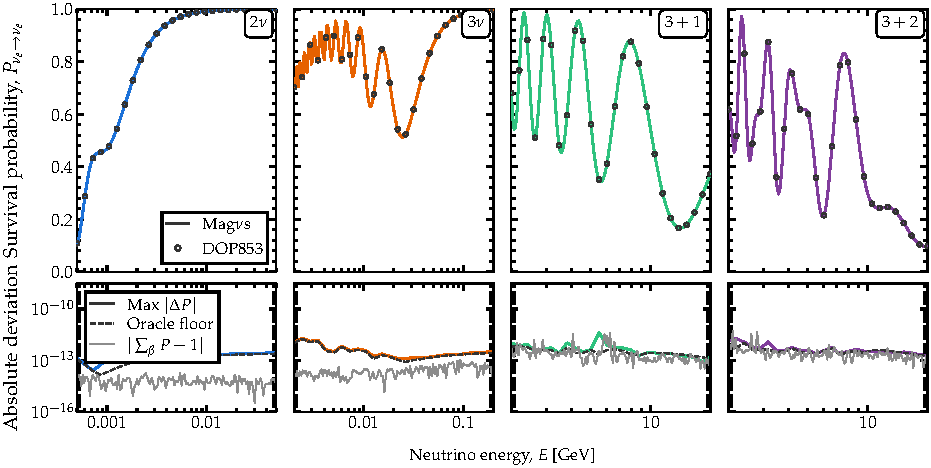
\includegraphics[width=\textwidth]{validation.pdf}
 \caption{\label{fig:validation}Survival probability $P_{\nu_e \to \nu_e}$ at two, three, four, and five flavors, along an exponentially falling density profile (central density $3 \cdot 10^{3}$~g~cm$^{-3}$, scale height $10$~km, baseline $25$~km). {\it Top}: the probability computed with \magnus\ \cite{Magnus} (solid) and with a {\tt DOP853} integration (eigth-order Runge-Kutta) of the same Hamiltonian. The profile is the same in every panel; the energy window differs, since an eV-scale $\Delta m^2_{41}$ and the standard mass splittings do not resonate at the same energy. {\it Bottom}: the largest deviation between the two over all entries of the probability matrix; the departure of each row of the matrix from summing to one; and the \emph{oracle floor}, the amount by which the {\tt DOP853} result itself changes when its tolerance is tightened from ${\tt rtol} = 10^{-12}$ to $10^{-13}$. Deviations below the floor cannot be resolved by this comparison. The sterile parameters are $\sin^2\theta_{14} = \sin^2\theta_{24} = 0.1$ and $\Delta m^2_{41} = 1$~eV$^2$, with $\sin^2\theta_{15} = \sin^2\theta_{25} = 0.06$ and $\Delta m^2_{51} = 1.7$~eV$^2$ at five flavors. Listing~\ref{lst:validation} shows the code to compute these curves. Every figure in this paper is computed in full in notebook \#28 (\ref{app:notebooks}).}
\end{figure*}
%%%%%%%%%%%%%%%%%%%%%%%%%%%%%%%%%%%%%%%%%%%%%%%%%%%%%

%%%%%%%%%%%%%%%%%%%%%%%%%%%%%%%%%%%%%%%%%%%%%%%%%%%%%
%%%%%%%%%%%%%%%%%%%%%%%%%%%%%%%%%%%%%%%%%%%%%%%%%%%%%

\section{Synopsis}
\label{sec:synopsis}

To address this, we introduce \magnus\ \cite{Magnus}\footnote{Install via {\tt pip install magnuspy}\;.  Tutorials at \Ref~\cite{MagnusDocs}.}, a code that returns oscillation probabilities for any Hamiltonian and any matter profile. \magnus\ is meant to spare its users from writing new code for each new setup or model. A new setup is a different baseline, energy range, or matter profile: a long-baseline beam, an atmospheric oscillogram, a solar or supernova signal. A new model is a different Hamiltonian: non-standard interactions, a sterile state, a long-range force. In \magnus, they are inputs; the probability is the output. We designed it to be as transparent as possible, so that its users can focus on the physics rather than on numerical optimization: \magnus\ chooses its own discretization and method from the Hamiltonian and a requested tolerance.

\magnus\ computes the evolution operator with the \textit{Magnus expansion}\ \cite{Magnus:1954zz, Blanes:2008xlr}: over a segment of the trajectory of the neutrino---within which the Hamiltonian may vary---the expansion writes the operator as a single exponential, $\mathbb{U} = \exp(\Omega)$, where $\Omega$ is a series of integrals of nested commutators of the Hamiltonian. Truncated at order $2n$ in the segment width ($n = 1, \dots, 5$ in \magnus), the series gives an error that falls as the $2n$-th power of that width. The staircase mentioned earlier is its second-order truncation; \magnus\ goes up to order 10.

Three advantages follow, independently of what the Hamiltonian contains: robustness, speed, and flexibility. \magnus\ is \emph{robust}: because the evolution operator is exactly unitary at any order, any tolerance, and any slab count, the probabilities add up to one to within numerical round-off. \magnus~is \emph{fast} without sacrificing accuracy: its cost follows the profile and not the phase, whereas a differential-equation solver pays for every radian resolved. A scan over neutrino energy or arrival direction is a single batched call, run on compiled {\tt Numba} kernels, rather than thousands of separate ones. And \magnus~is \emph{flexible}: the Hamiltonian is a callable returning a Hermitian matrix of any size, so five flavors, non-standard interactions, a Lorentz-violating background, and a completely novel neutrino interaction are one and the same call. 

Figure~\ref{fig:validation} shows the survival probability $P_{\nu_e \to \nu_e}$ of a neutrino crossing an exponentially falling density profile, computed with \magnus\ at two, three, four, and five flavors; the last two include one and two sterile states. The deviation from an independent integration of the same Hamiltonian---the {\tt DOP853} eigth-order Runge-Kotta solver---is a few parts in $10^{12}$, at the limit of that integration's own accuracy.

Listing~\ref{lst:validation} shows that generating the data for \figu{validation} takes only a few lines of code. Run as printed, Listing~\ref{lst:validation} takes about half a second on a laptop. It asks for ${\tt rtol} = 10^{-12}$ and ${\tt atol} = 10^{-14}$, far beyond what any oscillation analysis requires, only to match the comparison in \figu{validation}. At that tolerance it names its engine, the Magnus ladder at order eight (Secs.~\ref{sec:engines} and~\ref{sec:quadrature}), which is some fifteen times faster there than the default route; at the default of $10^{-3}$, the listing takes about 0.2~s, most of it one-time start-up. The listing calls four of the wrappers \magnus\ ships for the cases most often met, one per flavor count; the four calls differ only in the energy window and in the mixing parameters each count adds. The wrappers are a convenience: each builds a Hamiltonian internally and hands it to the core function of \magnus. A scenario for which \magnus\ ships no wrapper is the same call with a Hamiltonian of the user's own.

While the Magnus expansion is at the core of \magnus, the code does not rely on the expansion alone. Where the accumulated phase is extreme and the profile varies slowly, as in the Sun, \magnus\ transports the state along the instantaneous eigenstates of $\mathbb{H}$ and reserves the expansion for the narrow windows in which two eigenvalues approach and that transport fails. \magnus\ decides the hand-over from the Hamiltonian itself, with no intervention from the user.

\begin{lstlisting}[language=Python, caption={Computing the data in \figu{validation} with \magnus: the $\nu_e$ survival probability along an exponentially falling density profile at two, three, four (3+1), and five (3+2) flavors, one panel of \figu{validation} each. One wrapper serves each flavor count; the four calls differ only in the energy window and in the sterile mixing that the 3+1 and 3+2 cases add. The oscillation parameters are the NuFIT 6.1 best-fit values~\cite{Esteban:2024eli} (normal ordering, with Super-Kamiokande atmospheric data). The active-sterile mixing is $\sin^2\theta_{14} = \sin^2\theta_{24} = 0.1$ with $\Delta m_{41}^2 = 1$~eV$^2$ in both sterile cases, plus $\sin^2\theta_{15} = \sin^2\theta_{25} = 0.06$ with $\Delta m_{51}^2 = 1.7$~eV$^2$ in the 3+2 case; every other active-sterile parameter is zero. The tolerances, ${\tt rtol} = 10^{-12}$ and ${\tt atol} = 10^{-14}$, are those of the comparison in \figu{validation}. (The defaults are $10^{-3}$; here they are tightened to match the comparison in \figu{validation}.)}, label={lst:validation}, float=t]
import numpy as np
import magnus.globaldefs as gd
import magnus.oscprob as oscprob

# Standard oscillation parameters
osc = gd.load_nufit_params('NuFIT 6.1')
# Active-sterile mixing
s14 = s24 = np.sqrt(0.10)
s15 = s25 = np.sqrt(0.06)

def energies(lo, hi):
    return np.logspace(np.log10(lo), np.log10(hi),
                       140)*gd.UNIT_GEV

# Exponentially falling density: 3e3 g/cm^3 at the
# origin, scale height 10 km, 25 km baseline.
# Every mixing parameter left out defaults to zero.
common = dict(L=25.0*gd.UNIT_KM, L0=0.0,
              rho_central=3.e3,
              l_scale=10.0*gd.UNIT_KM,
              density_matter_is_in_g_per_cm3=True,
              nu_i=gd.NUE, nu_f=gd.NUE,
              rtol=1e-12, atol=1e-14,
              strategy='magnus', magnus_exp_order=8)

P_2nu = oscprob.osc_prob_2nu_matter_exp_density(
    energies(0.0005, 0.05), **common,
    sth=osc['s12'], Dm2=osc['D21'])

P_3nu = oscprob.osc_prob_3nu_matter_exp_density(
    energies(0.002, 0.2), **common, **osc)

P_4nu = oscprob.osc_prob_4nu_matter_exp_density(
    energies(2.0, 20.0), **common, **osc,
    s14=s14, s24=s24, D41=1.0)

P_5nu = oscprob.osc_prob_5nu_matter_exp_density(
    energies(2.0, 20.0), **common, **osc,
    s14=s14, s15=s15, s24=s24, s25=s25,
    D41=1.0, D51=1.7)
\end{lstlisting}

\magnus~ships ready-made cases for the scenarios most often explored: propagation in vacuum, in matter of constant or exponentially falling density, through the Earth, and through the Sun, on an exponential fit or on any of twelve standard solar models. Each case comes with standard oscillations and with new physics: non-standard neutrino-matter interactions, Lorentz-invariance violation, sterile neutrinos, and pseudo-Dirac neutrinos. The ready-made cases span two to five flavors (three active and up to two sterile); the generic functions take any number. Any other profile, such as a supernova shock front, is a function the user passes in.

Beyond the oscillation probability, \magnus~returns the \emph{phase-averaged} probability, \ie, the probability with each interference term damped by the spread of its phase across the energy resolution of the measurement. Where a phase runs through many cycles, as for a solar or an astrophysical neutrino, this is the $L/E \to \infty$ limit, with $E$ the neutrino energy. Every function can also return the evolution operator $\mathbb{U}$ alongside the probabilities. Every function can also return the evolution operator $\mathbb{U}$ alongside the probabilities. The probabilities keep only the magnitudes of the transition amplitudes; the operator keeps their phases too. The phases are needed, for example, to compute the probability that a neutrino leaving a star arrives in each mass eigenstate rather than in each flavor.

\magnus~ships functions that draw commonly used plots: probability against distance or energy, oscillograms, and bi-probability plots. A command-line tool lets the user run \magnus\ as a calculator: it returns the probabilities for one energy and baseline without writing code. The application programming interface (API) is fully documented and publicly available~\cite{MagnusDocs}, along with implementation details and tutorial notebooks.

The rest of the paper is organized as follows. Section~\ref{sec:recap} fixes notation. Section~\ref{sec:method} presents the method. Section~\ref{sec:code} describes the code. Section~\ref{sec:examples} shows it in use. Section~\ref{sec:performance} measures its speed, precision, and reach. Section~\ref{sec:comparison} compares it against two other public codes, with each case checked by a third, independent method. Section~\ref{sec:conclusions} concludes. The appendices contain supporting detail: the Magnus expansion at any order, the predefined oscillation-parameter sets, the test suite, and the notebooks.

%%%%%%%%%%%%%%%%%%%%%%%%%%%%%%%%%%%%%%%%%%%%%%%%%%%%%
%%%%%%%%%%%%%%%%%%%%%%%%%%%%%%%%%%%%%%%%%%%%%%%%%%%%%

\section{Neutrino oscillations: units, notation, conventions}
\label{sec:recap}

In a system of $n \geq 2$ neutrino flavors, $\nu_\alpha$ is the flavor state of a neutrino, represented by an $n$-component column vector, and $\mathbb{H}$ is the $n \times n$ Hamiltonian in flavor space. We use natural units, $c = \hbar = 1$, with energies in eV and distances in eV$^{-1}$, so that $\mathbb{H}L$ is dimensionless. Every length an oscillation function takes is in eV$^{-1}$: baselines, radii, slab edges, and breakpoints alike. Multiplying by {\tt globaldefs.UNIT\_KM} converts km into eV$^{-1}$; 1~km is about $5.07 \cdot 10^{9}$~eV$^{-1}$. (Earth-geometry helpers, such as {\tt earth.distance\_traveled\_inside\_earth}, work in km instead, so their output must be converted before it is passed on.) Passing a length that is not in eV$^{-1}$ raises no error: a baseline passed in km is read as a few mm, yet the call returns a converged, unitary probability. \magnus\ does warn when a baseline is short enough to be km left unconverted, but does not halt.

Because neutrinos are relativistic, we identify the elapsed time with the distance traveled and write both as $l$. The state obeys \equ{schrodinger}; its solution defines the evolution operator $\mathbb{U}(l_1, l_0)$  through $\nu_\alpha(l_1) = \mathbb{U}(l_1,l_0)\, \nu_
\alpha(l_0)$, with $\mathbb{U}(l_0,l_0) = \mathbb{1}$. The probability that a neutrino born as $\nu_\alpha$ is detected as $\nu_\beta$ is
\begin{equation}
 \label{equ:probability}
 P_{\nu_\alpha \to \nu_\beta}(l_1, l_0)
 =
 \left\lvert \left[\mathbb{U}(l_1,l_0)\right]_{\beta\alpha} \right\rvert^2 \;.
\end{equation}
We take $\mathbb{H}$ Hermitian throughout; $\mathbb{U}$ is then unitary and $\sum_\beta P_{\nu_\alpha \to \nu_\beta} = 1$ for every $\alpha$. Flavor indices run over $e, \mu, \tau$ at $n=3$ and over $e, \mu, \tau, s_1$ at $n = 4$ and $e, \mu, \tau, s_1, s_2$ at $n = 5$, the states $s_i$ being sterile, which interact only through their mixing.

As an example, in vacuum, the Hamiltonian is
\begin{equation}
 \label{equ:h_vacuum}
 \mathbb{H}^{\rm vac}(E)
 =
 \frac{1}{2E}\, \mathbb{R}\, \mathbb{M}^2\, \mathbb{R}^\dagger \;,
\end{equation}
where $\mathbb{M}^2 = {\rm diag}(0, \Delta m^2_{21}, \Delta m^2_{31}, \ldots)$, $\Delta m^2_{ij} \equiv m_i^2 - m_j^2$, $m_i$ and $m_j$ are the masses of the neutrino mass eigenstates $\nu_i$ and $\nu_j$, and $\mathbb{R}$ is the mixing matrix that rotates between the flavor and mass bases.  The matrix is parametrized by the rotation angles and CP-violation phases. At three flavors---the standard case with $\nu_e$, $\nu_\mu$, $\nu_\tau$---it corresponds to the Pontecorvo-Maki-Nakagawa-Sakata (PMNS) mixing matrix, parametrized in terms of three mixing angles, $\theta_{12}$, $\theta_{23}$, and $\theta_{13}$, and one phase, $\delta_{\rm CP}$. 

In \magnus, $\mathbb{R}$ is a product of rotations. Each $\mathbb{R}_{ij}$ rotates by an angle $\theta_{ij}$ in the $(i,j)$ plane: it has $\cos\theta_{ij}$ in entries $(i,i)$ and $(j,j)$, $\sin\theta_{ij}\,e^{-i\delta_{ij}}$ in entry $(i,j)$, $-\sin\theta_{ij}\,e^{i\delta_{ij}}$ in entry $(j,i)$, ones in the remaining diagonal entries, and zeros in all other entries. For instance, at three flavors,
\begin{equation}
 \label{equ:rotation_example}
 \mathbb{R}_{13}
 =
 \begin{pmatrix}
  \cos\theta_{13} & 0 & \sin\theta_{13}\, e^{-i\delta_{13}} \\
  0 & 1 & 0 \\
  -\sin\theta_{13}\, e^{i\delta_{13}} & 0 & \cos\theta_{13}
 \end{pmatrix} \;.
\end{equation}
For $n$ flavors,
\begin{equation}
 \label{equ:mixing_matrix}
 \mathbb{R}
 =
 \begin{cases}
  \mathbb{R}_{12} \;, & n = 2 \;, \\
  \mathbb{R}_{23}\, \mathbb{R}_{13}\, \mathbb{R}_{12} \;, & n = 3 \;, \\
  \mathbb{R}_{34}\, \mathbb{R}_{24}\, \mathbb{R}_{14}\, \mathbb{R}_{23}\, \mathbb{R}_{13}\, \mathbb{R}_{12} \;, & n = 4 \;, \\
  \mathbb{R}_{35}\, \mathbb{R}_{25}\, \mathbb{R}_{15}\, \mathbb{R}_{34}\, \mathbb{R}_{24}\, \mathbb{R}_{14}\, \mathbb{R}_{23}\, \mathbb{R}_{13}\, \mathbb{R}_{12} \;, & n = 5 \;.
 \end{cases}
\end{equation}
At $n = 2$, $\mathbb{R}_{12}$ is a real rotation by the single mixing angle $\theta$. At $n \geq 3$, the phase of $\mathbb{R}_{13}$ is $\delta_{13} \equiv \delta_{\rm CP}$. Each sterile state adds its rotations on the left, and of these only $\mathbb{R}_{14}$, $\mathbb{R}_{24}$, $\mathbb{R}_{15}$, and $\mathbb{R}_{35}$ carry a phase. All other rotations are real. There is no $\mathbb{R}_{45}$: a rotation between the two sterile states only relabels them, since both feel the same potential, and it leaves every probability between active flavors unchanged.

Flavor indices run over $e$, $\mu$ at $n = 2$ (changeable; see Sec.~\ref{sec:two_flavors}); $e$, $\mu$, $\tau$ at $n = 3$; $e$, $\mu$, $\tau$, $s_1$ at $n = 4$; and $e$, $\mu$, $\tau$, $s_1$, $s_2$ at $n = 5$. (\magnus\ accepts an arbitrary number of flavors, but examples in this paper---save for pseudo-Dirac neutrinos---stop at five.) The sterile states $s_i$ feel no weak interaction; they take part in oscillations only through their mixing with active ones.

In matter, neutrinos scatter coherently forward on electrons via charged-current (CC) interactions and on electrons, protons, and neutrons via neutral-current (NC) ones. As a result, the Hamiltonian acquires the Mikheev-Smirnov-Wolfenstein (MSW) term\ \cite{Wolfenstein:1977ue, Mikheev:1986gs}
\begin{equation}
 \label{equ:h_matter}
 \mathbb{H}(E, l)
 =
 \mathbb{H}^{\rm vac}(E)
 +
 V_{\rm CC}(l)\, \mathbb{P}(l) \;,
 \quad
 V_{\rm CC} = \sqrt{2}\, G_F\, n_e(l) \;,
\end{equation}
where $V_{\rm CC}$ is the matter potential, $n_e$ is the electron number density, $G_F$ is the Fermi constant, and $\mathbb{P}$, the projector, is a diagonal matrix. The projector is where the flavor count enters. 

At three flavors, $\mathbb{P} = {\rm diag}(1,0,0)$: the neutral-current (NC) potential is common to the three active flavors and cancels from the probabilities. With a sterile state, it no longer cancels, since a sterile neutrino is a gauge singlet and feels neither potential. In this case, $\mathbb{P} = {\rm diag}(1, 0, 0, r/2, \ldots)$ with $r = n_n/n_p$ the ratio of neutrons to protons. The $r/2$ factor is explained as follows. The NC potential of an active flavor is $V_{\rm NC} = -G_F n_n/\sqrt{2}$. Subtracting it from the whole diagonal is what removes it from the active flavors; what it leaves on a sterile state is $-V_{\rm NC}$. With $n_p = n_e$ by charge neutrality, $-V_{\rm NC} = G_F n_n/\sqrt{2} = (n_n/n_p)\,G_F n_e/\sqrt{2} = (r/2)\,V_{\rm CC}$. So the sterile entry is not an interaction of the sterile state but the residue of the subtraction: $1/2$ for isoscalar matter (\ie, matter with $n_n = n_p$). For every flavor count, \magnus\ builds $\mathbb{P}$ in {\tt matter.matter\_potential\_projector}. The wrappers take $r$ as {\tt ratio\_number\_neutrons\_to\_protons}, a number or a function of position, $r(l)$. Earth wrappers use the latter to follow the composition of each layer, so $\mathbb{P}$ varies along the path.

For antineutrinos, the mixing matrix is conjugated \emph{and} the matter potential changes sign. Doing only one of the two returns a plausible but wrong answer, so the wrappers take a {\tt nubar} flag that does both instead of leaving it to the user.

%%%%%%%%%%%%%%%%%%%%%%%%%%%%%%%%%%%%%%%%%%%%%%%%%%%%%
%%%%%%%%%%%%%%%%%%%%%%%%%%%%%%%%%%%%%%%%%%%%%%%%%%%%%

\section{The method}
\label{sec:method}

%%%%%%%%%%%%%%%%%%%%%%%%%%%%%%%%%%%%%%%%%%%%%%%%%%%%%

\subsection{History and context}

The Magnus expansion is due to Magnus\ \cite{Magnus:1954zz}. In numerical analysis, it is one of the standard geometric integrators: methods that preserve a structure of the problem, here unitarity, exactly rather than to within the truncation error\ \cite{Iserles:2000acta, Hairer:2006gni}. \Ref\ \cite{Blanes:2008xlr} reviews it. By default, \magnus\ evaluates it with the Gauss-Legendre \emph{collocation} integrators of \Refs\ \cite{Blanes:2000bit, Blanes:2002opt}: the Hamiltonian is sampled at a few Gauss-Legendre nodes inside each step, and the scheme is built so that those samples deliver the full order. We introduce them below.

The Magnus expansion has been used for neutrino oscillations before. D'Olivo and Oteo brought it to two-flavor evolution in matter\ \cite{DOlivo:1990xs}, Ioannisian and Smirnov developed it for realistic profiles\ \cite{Ioannisian:2008ve}, and Casas \emph{et al.}\ turned it into a practical integrator for three flavors\ \cite{Casas:2016asi}, reporting gains of up to two orders of magnitude in speed over general-purpose solvers.

What has been missing is not a method but its engineering: a general-purpose, tested, and documented implementation that can be used for a wide range of physics studies with minimal supervision, which \magnus\ provides. It takes an arbitrary Hermitian Hamiltonian at any number of flavors, on a continuous or a layered profile, and chooses its own discretization of the path from a requested tolerance, aligned with any discontinuities. For each request for a probability, it chooses among several ways of computing the answer, suited to different kinds of Hamiltonian (Sec.~\ref{sec:engines}), and reports which one it used. When it cannot confirm that its answer has converged, it warns instead of returning it silently. It implements the Magnus expansion up to ten terms, two quadrature rules, the composition of the path in steps and its adaptive refinement, an exactly unitary matrix exponential, adiabatic transport with Magnus patches, the phase-averaged probability, and batching, which makes a scan over energy or arrival direction one call instead of thousands.

%%%%%%%%%%%%%%%%%%%%%%%%%%%%%%%%%%%%%%%%%%%%%%%%%%%%%

\subsection{Where the method applies and where it does not}
\label{sec:applicability}

The method, and its implementation in \magnus, require one thing only: \textbf{that the Hamiltonian be Hermitian}. Hermiticity makes the evolution unitary and the system closed, so that the total probability, summed over all flavors, is conserved. Section~\ref{sec:limitations} lists the cases this excludes, among them open systems such as invisible neutrino decay and decoherence; for those, other codes should be used, such as \texttt{nuSQuIDS}~\cite{Arguelles:2021twb, NuSQuIDS}.

Convergence of the Magnus expansion is not a second requirement on the user: \magnus\ handles it internally. The series, introduced formally in Sec.~\ref{sec:expansion}, converges absolutely if $\int \lVert \mathbb{H} \rVert_2\, dl < \pi$ over the interval it is applied to\ \cite{Moan:2008conv}, where $\lVert \cdot \rVert_2$ is the spectral norm, which for a Hermitian matrix is its largest eigenvalue in modulus. The condition is sufficient, not necessary, so a particular $\mathbb{H}$ may converge well beyond it; but no constant larger than $\pi$ guarantees convergence for every $\mathbb{H}$. Over a long path the integral exceeds $\pi$, so \magnus\ cuts the path into \emph{slabs}, applies the expansion on each, and composes the results (Sec.~\ref{sec:order_is_the_slab_product}). The number and positions of the slabs follow from the requested tolerance: \magnus\ refines them until successive results agree (Sec.~\ref{sec:refinement}), without user intervention. (The user may instead fix the slabs.) If a slab still exceeds the bound, \magnus\ warns; if the requested tolerance is not reached, because, \eg, the cap on the number of slabs is too low, it reports that too.

%%%%%%%%%%%%%%%%%%%%%%%%%%%%%%%%%%%%%%%%%%%%%%%%%%%%%

\subsection{The Magnus expansion}
\label{sec:expansion}

Writing $\mathbb{A}(l) \equiv -i\,\mathbb{H}(l)$, \equ{schrodinger} reads $d\mathbb{U}/dl = \mathbb{A}(l)\,\mathbb{U}$. Where $\mathbb{A}$ commutes with itself at different positions (for neutrinos, in vacuum or at uniform density), the solution is $\exp \left( \int \mathbb{A}\,dl \right)$; where it does not, that expression is wrong. The time-ordered exponential that replaces it is the Magnus expansion\ \cite{Magnus:1954zz}:
\begin{equation}
 \label{equ:magnus}
 \mathbb{U}(l, l_0) = \exp\left[\Omega(l, l_0)\right] \;,
 \qquad
 \Omega = \sum_{k \geq 1} \Omega_k \;,
\end{equation}
exactly wherever the series converges (Sec.~\ref{sec:applicability}), with the terms generated by a recursion in the Bernoulli numbers $B_j$ (in the $B_1 = -1/2$ convention)\ \cite{Blanes:2008xlr},
\begin{equation}
 \label{equ:recursion}
 \Omega_1 = \int_{l_0}^{l} \mathbb{A}\,ds \;,
 \quad
 \Omega_k = \sum_{j=1}^{k-1} \frac{B_j}{j!} \int_{l_0}^{l} S_k^{(j)}\, ds \;,
\end{equation}
where $S_k^{(1)} = [\Omega_{k-1}, \mathbb{A}]$ and $S_k^{(j)} = \sum_{m=1}^{k-j} [\Omega_m, S_{k-m}^{(j-1)}]$. The time-ordering means that the earlier-time operators are applied first, \ie, are positioned to the right of later-time operators.

The first three terms read
\begin{align}
 \label{equ:omega123}
 \Omega_1 &= \int_{l_0}^{l}\! ds\, \mathbb{A}(s) \;, \nonumber \\
 \Omega_2 &= \frac{1}{2}\int_{l_0}^{l}\! ds_1 \int_{l_0}^{s_1}\! ds_2\,
 \left[\mathbb{A}(s_1), \mathbb{A}(s_2)\right] \;, \\
 \Omega_3 &= \frac{1}{6}\int_{l_0}^{l}\! ds_1 \int_{l_0}^{s_1}\! ds_2
 \int_{l_0}^{s_2}\! ds_3 \Big(
 \left[\mathbb{A}_1, [\mathbb{A}_2, \mathbb{A}_3]\right] \nonumber \\
 &\hspace{3.1cm} + \left[\mathbb{A}_3, [\mathbb{A}_2, \mathbb{A}_1]\right]
 \Big) \;, \nonumber
\end{align}
with $\mathbb{A}_i \equiv \mathbb{A}(s_i)$. \ref{app:terms} gives the structure at any order. The odd Bernoulli numbers vanish for $j \geq 3$, so whole commutator groups drop out and only $j = 1, 2, 4, 6, \ldots$ contribute. Every term unrolls to a right-nested chain $[\Omega_{m_1}, [\Omega_{m_2}, \ldots [\Omega_{m_j}, \mathbb{A}]\ldots]]$ with $\sum_i m_i = k-1$, so the terms of the $j$-th group are indexed by the compositions of $k-1$ into $j$ positive parts and there are $\binom{k-2}{j-1}$ of them. Their number roughly doubles per order: $\Omega_7$ has $17$ terms and $\Omega_{10}$ has $129$.

In neutrino oscillations, the first term of the Magnus expansion is the one driving the standard slab approximation. Where $\mathbb{H}$ does not depend on position, $\Omega_1 = -i\mathbb{H}\Delta l$ is the whole of the expansion, since every higher term is a nested commutator of $\mathbb{H}$ with itself and vanishes identically. Its exponential is then the exact evolution operator, not a truncation of one. Evaluating it is the problem {\tt NuOscProbExact}\ \cite{NuOscProbExact, Bustamante:2019ggq} solves, for up to four flavors: expanding $\mathbb{H}$ and $e^{-i\mathbb{H}L}$ in the generators of SU($n$) returns the probability from the eigenvalues of $\mathbb{H}$ and traces alone, without ever constructing an eigenvector. The eigenvalues are found in closed form at two and three flavors and numerically at four. Composing one such operator per slab, in the order the neutrino meets them, is the standard slab treatment of a piecewise-constant profile~\cite{Akhmedov:1988kd, Krastev:1989ix, Akhmedov:1998ui}. We take that correspondence further in Sec.~\ref{sec:order_is_the_slab_product}.

\magnus\ implements \equ{recursion} through $\Omega_{10}$. The terms through $\Omega_6$ are written out in the simplified forms of \Ref\ \cite{Blanes:2008xlr}, and those beyond are generated from the recursion. The terms through $\Omega_6$ are written out in the simplified forms of \Ref\ \cite{Blanes:2008xlr}, and those beyond are generated from the recursion. A separate module, {\tt expansionterms}, derives the same terms symbolically, in exact rational arithmetic, at \emph{any} order, and shares no code with the numerical core. The test suite checks the two against each other, term by term through $\Omega_{10}$, and regenerates the hard-coded recursion coefficients (\ref{app:tests}). (Users interested in applying the Magnus expansion to other problems---in magnetic resonance, quantum optics, lattice gauge theory, or condensed matter---may repurpose {\tt expansionterms}.)

%%%%%%%%%%%%%%%%%%%%%%%%%%%%%%%%%%%%%%%%%%%%%%%%%%%%%

\subsection{Truncation is exactly unitary}
\label{sec:unitarity}

Because $\mathbb{H}$ is Hermitian, $\mathbb{A} = -i\mathbb{H}$ is anti-Hermitian, and the commutator of two anti-Hermitian matrices is again anti-Hermitian. Every $\Omega_k$ in \equ{recursion} is a combination, with real coefficients, of nested commutators of $\mathbb{A}$ with itself, so every $\Omega_k$ is anti-Hermitian, and so is any partial sum. Therefore,
\begin{equation}
 \label{equ:unitary}
 \Omega^\dagger = -\Omega
 \quad\Longrightarrow\quad
 \left[\exp(\Omega)\right]^\dagger \exp(\Omega) = \mathbb{1}
\end{equation}
for \emph{every} truncation order and every quadrature accuracy. Truncating early costs accuracy, never unitarity. This is the sense in which the method is a geometric integrator: the exact solution lies in the unitary group, and so does every approximation to it. Neither truncating the series nor evaluating its integrals numerically leaves the group, so $\exp(\Omega)$ is unitary at any setting, not only in the limit of a fine discretization.

In practice, the guarantee is only as good as the routine that computes the exponential. A general-purpose Pad\'e routine knows nothing of the structure of its argument, and returns a matrix that is unitary only to its own error tolerance, so the exactness would be lost at the last step. \magnus\ instead uses a form that is unitary by construction. Because $\Omega$ is anti-Hermitian, $\mathbb{K} \equiv i\Omega$ is Hermitian, so it is diagonalized by a unitary $\mathbb{V}$, and
\begin{align}
 \mathbb{K} &= \mathbb{V}\, {\rm diag}(\lambda_1, \ldots, \lambda_n)\, \mathbb{V}^\dagger \;, \nonumber \\
 \label{equ:expm}
 \exp(\Omega) &= \mathbb{V}\, {\rm diag}\!\left(e^{-i\lambda_1}, \ldots, e^{-i\lambda_n}\right) \mathbb{V}^\dagger \;,
\end{align}
where the eigenvalues $\lambda_1, \ldots, \lambda_n$ of $\mathbb{K}$ are real. The middle factor is therefore a diagonal of pure phases, and conjugating it by a unitary $\mathbb{V}$ keeps it unitary: $\exp(\Omega)$ is unitary by its form, not to the accuracy of an approximation. Section~\ref{sec:exponential} describes how \magnus\ evaluates \equ{expm}: in closed form at two and three flavors, with a compiled eigensolver at four and five, and with a general Hermitian eigendecomposition above five.

In floating-point arithmetic, neither route is unitary to the last bit, because $\mathbb{V}$ is itself computed with rounding. Two measurements show how close it comes, and they measure different things. A single exponential deviates by $\lVert \mathbb{U}^\dagger \mathbb{U} - \mathbb{1}\rVert = 4 \cdot 10^{-16}$ in the median; over a stack of $4096$, the worst reaches $4 \cdot 10^{-15}$ while the median stays put, so a larger workload lengthens the tail without moving the typical case. A probability is built from many such factors, so its deviation grows with their number: across four decades in the number of points, at two through five flavors, the worst case grows from $3 \cdot 10^{-12}$ to $1.6 \cdot 10^{-11}$. For all practical purposes, \magnus\ preserves unitarity.

%%%%%%%%%%%%%%%%%%%%%%%%%%%%%%%%%%%%%%%%%%%%%%%%%%%%%

\subsection{Two quadrature rules for the Magnus expansion}
\label{sec:quadrature}

Evaluating the Magnus recursion, \equ{recursion}, means sampling $\mathbb{A}$ inside each slab; \magnus\ offers two families of quadrature rule to approximate the integrals in the recursion.

\smallskip

\textit{Collocation integrators (default).---}By default \magnus\ does not evaluate \equ{recursion} as it stands. Each $\Omega_k$ there is a $k$-fold integral over $(k-1)$-fold nested commutators, so the integration and the commutator count both grow steeply with $k$; the sixth-order truncation alone would call for four such integrals. The collocation rules presented below replace them. They define $\Omega_{\rm GL}^{(p)}$, each of which is a quadrature approximation to a \emph{truncation} of the Magnus series in \equ{magnus}, assembled from a few samples of $\mathbb{A}$ at Gauss-Legendre nodes across a slab width, $h$, together with a fixed set of commutators among those samples. Its label is the order $p$ that it attains, not the number of terms that it keeps, \ie,
\begin{equation}
 \label{equ:gl_definition}
 \Omega_{\rm GL}^{(p)}
 =
 \sum_{k=1}^{m_p} \Omega_k + \mathcal{O}\!\left(h^{p+1}\right) \;,
\end{equation}
where $m_p = 1,\, 2,\, 4,\, 6$ for $p = 2,\, 4,\, 6,\, 8$, with $p$ always even. The error in \equ{gl_definition} comes from the next pair of Magnus terms of \equ{magnus}, which is what fixes the order at $p$.  \ref{app:terms} derives the sets of Magnus commutators retained in the collocation integrators and the required evenness of $p$.  (While the construction of collocation integrators is not unique to Gauss-Legendre quadrature, collocation terms written under different quadrature schemes cannot be interchanged or mixed.)

What the collocation provides is economy of computation: for a given truncation of the Magnus series in \equ{magnus}, fewer commutators and instances of the Hamiltonian need to be evaluated via collocation compared to the straightforward application of the series, as we show below. It is the cheapest route to a given accuracy whenever $\mathbb{H}$ is smooth inside a slab. This is the case, \eg, inside the Earth, where the density is smooth between layer boundaries and \magnus\ puts the slab edges on the boundaries themselves (Sec.~\ref{sec:refinement}).

We use $\Omega_{\rm GL}^{(p)}$ as \equ{magnus} uses $\Omega$. On the $j$-th slab, spanning $l_{j-1}$ to $l_j$ with width $h = l_j - l_{j-1}$, the evolution operator is
\begin{equation}
 \label{equ:slab_exponential}
 \mathbb{U}_j = \exp\left[\Omega_{\rm GL}^{(p)}(l_j, l_{j-1})\right] \;,
\end{equation}
one matrix exponential per slab, with the $\mathbb{U}_j$ time-ordered. Like for the Magnus series itself (see Sec.~\ref{sec:unitarity}), truncating the series $\Omega_{\rm GL}^{(p)}$ inside the exponential leaves $\mathbb{U}_j$ exactly unitary.

Following \Refs\ \cite{Blanes:2000bit, Blanes:2002opt}, Magnus orders 2, 4, 6, and 8 are reached from only one, two, three, or four evaluations of $\mathbb{A}$ per slab, taken at the Gauss-Legendre nodes. \magnus\ implements all four. 
(These are \textit{not} the commutator-free family of \Refs\ \cite{Blanes:2006cf, Alvermann:2011cf}, which replaces commutators by products of exponentials of linear combinations of the $\mathbb{A}_i$.) With $\mathbb{A}_j \equiv -i \mathbb{H}_j$ the Hamiltonian at node $j$, the collocation integrators are
\begin{align}
 \label{equ:gl}
 \Omega_{\rm GL}^{(2)} &= h\, \mathbb{A}_1 \;, \nonumber \\
 \Omega_{\rm GL}^{(4)} &= \frac{h}{2}\left(\mathbb{A}_1 + \mathbb{A}_2\right)
 + \frac{\sqrt{3}}{12}\, h^2 \left[\mathbb{A}_2, \mathbb{A}_1\right] \;, \nonumber \\
 \Omega_{\rm GL}^{(6)} &= \alpha_1 + \frac{\alpha_3}{12}
 + \frac{1}{240} \left[-20\,\alpha_1 - \alpha_3 + \mathbb{C}_1,\,
 \alpha_2 + \mathbb{C}_2\right] \;, \nonumber \\
 \Omega_{\rm GL}^{(8)} &= \alpha_1 + \frac{\alpha_3}{12}
 - \frac{7}{120}\,\mathbb{C}_3 + \frac{1}{360}\,\mathbb{C}_6 \;.
\end{align}
Orders 2 and 4 follow \Ref\ \cite{Blanes:2000bit}; orders 6 and 8 are the commutator-optimized forms of \Ref\ \cite{Blanes:2002opt}, the order-6 one also reproduced in the review of \Ref\ \cite{Blanes:2008xlr}. Orders 4, 6, and 8 need 1, 3, and 6 commutators, the fewest possible at each order\ \cite{Blanes:2002opt}. \tabl{collocation} collects the $\alpha_i$ and the $\mathbb{C}_i$ that build the last two of \equ{gl}; the two columns are different objects on different nodes, and cannot be mixed.

(We have found no collocation scheme of this form at order 10 or above. Reference\ \cite{Blanes:2000bit} only tabulates the size of the order-10 problem---80 determining equations after time-symmetry, against 27 at order 8; \Refs\ \cite{Blanes:2002opt, Blanes:2008xlr} stop at order 8. The commutator-free family does not reach higher either, \Refs\ \cite{Blanes:2006cf, Alvermann:2011cf} optimizing up to order 8 as well. Order 8 appears to be where the optimized literature ends. However, given how little order 8 gains over order 6 in \figu{smooth_reach} later, order 10 would rarely be worth reaching for in neutrino oscillation probabilities.)

%%%%%%%%%%%%%%%%%%%%%%%%%%%%%%%%%%%%%%%%%%%%%%%%%%%%%
\begin{table*}[t!]
 {\small
 \begin{tabular}{@{}l l l@{}}
  & Order 6, 3 GL nodes & Order 8, 4 GL nodes \\
 \hline
 $\alpha_1$ & $h\, \mathbb{A}_2$
            & $\frac{h}{2}\left[\left(\frac{1}{2} - \frac{\sqrt{30}}{8}\right)\mathbb{S}_1
              + \left(\frac{1}{2} + \frac{\sqrt{30}}{8}\right)\mathbb{S}_2\right]$ \\[2pt]
 $\alpha_2$ & $\frac{\sqrt{15}}{3}\, h \left(\mathbb{A}_3 - \mathbb{A}_1\right)$
            & $3h\left[(5 - \sqrt{30})\, d_1 \mathbb{R}_1 + (5 + \sqrt{30})\, d_2 \mathbb{R}_2\right]$ \\[2pt]
 $\alpha_3$ & $\frac{10}{3}\, h \left(\mathbb{A}_3 - 2\mathbb{A}_2 + \mathbb{A}_1\right)$
            & $\frac{7\sqrt{30}}{12}\, h \left(\mathbb{S}_1 - \mathbb{S}_2\right)$ \\[2pt]
 $\alpha_4$ & ---
            & $20h\left[(\sqrt{30} - 3)\, d_1 \mathbb{R}_1 - (3 + \sqrt{30})\, d_2 \mathbb{R}_2\right]$ \\
 \hline
 $\mathbb{C}_1$ & $\left[\alpha_1, \alpha_2\right]$
   & $-\frac{1}{28}\left[\alpha_1 + \frac{1}{28}\alpha_3 ,\; \alpha_2 + \frac{3}{28}\alpha_4\right]$ \\[2pt]
 $\mathbb{C}_2$ & $-\frac{1}{60}\left[\alpha_1, 2\alpha_3 + \mathbb{C}_1\right]$
   & $\frac{1}{3}\left[\alpha_1 ,\; -\frac{1}{14}\alpha_3 + \mathbb{C}_1\right]$ \\[2pt]
 $\mathbb{C}_3$ & ---
   & $\left[\alpha_1 + \frac{1}{28}\alpha_3 + \mathbb{C}_1 ,\; \alpha_2 + \frac{3}{28}\alpha_4 + \mathbb{C}_2\right]$ \\[2pt]
 $\mathbb{C}_4$ & --- & $\left[\alpha_2 , \mathbb{C}_1\right]$ \\[2pt]
 $\mathbb{C}_5$ & ---
   & $\left[\alpha_1 + \frac{5}{4}\mathbb{C}_1 ,\; 2\alpha_3 + \mathbb{C}_3 + \frac{1}{2}\mathbb{C}_4\right]$ \\[2pt]
 $\mathbb{C}_6$ & ---
   & $\left[\alpha_1 + \frac{1}{12}\alpha_3 - \frac{7}{3}\mathbb{C}_1 - \frac{1}{6}\mathbb{C}_3 ,\;
      -9\alpha_2 - \frac{9}{4}\alpha_4 + 63\,\mathbb{C}_2 + \mathbb{C}_5\right]$ \\
 \end{tabular}}
 \caption{\label{tab:collocation}The quantities entering the collocation integrators of \equ{gl}. The two columns are different objects on different Gauss-Legendre (GL) nodes and cannot be mixed: order 6 samples $\mathbb{A}$ at the slab midpoint and at $(\frac{1}{2} \pm \frac{\sqrt{15}}{10})h$; order 8 at $(\frac{1}{2} \pm v_1)h$ and $(\frac{1}{2} \pm v_2)h$, with $v_1 = \frac{1}{2}\sqrt{(3 + 2\sqrt{6/5})/7}$ and $v_2 = \frac{1}{2}\sqrt{(3 - 2\sqrt{6/5})/7}$. At order 8 the corresponding weights are $w_1 = \frac{1}{2} - \frac{1}{6}\sqrt{5/6}$ and $w_2 = \frac{1}{2} + \frac{1}{6}\sqrt{5/6}$, and we write $d_i \equiv w_i v_i$, $\mathbb{S}_1 = \mathbb{A}_1 + \mathbb{A}_4$, $\mathbb{S}_2 = \mathbb{A}_2 + \mathbb{A}_3$, $\mathbb{R}_1 = \mathbb{A}_4 - \mathbb{A}_1$, $\mathbb{R}_2 = \mathbb{A}_3 - \mathbb{A}_2$}
\end{table*}
%%%%%%%%%%%%%%%%%%%%%%%%%%%%%%%%%%%%%%%%%%%%%%%%%%%%%

\smallskip

\textit{Cumulative quadrature.---}The alternative rule to collocation is cumulative quadrature. Here, \magnus\ samples $\mathbb{A}$ on a uniform grid of $m$ points inside each slab and integrates with the trapezoid or Simpson rule, selectable; $m$ starts at 100 and the refinement adjusts it together with the number of slabs. The points are $s_i = l_{j-1} + i\,\Delta s$, spaced by $\Delta s = h/(m-1)$. Keeping the first $k$ terms of the series gives
\begin{equation}
 \label{equ:cum_definition}
 \Omega_{\rm cum}^{(k)}
 =
 \sum_{q=1}^{k} \widehat{\Omega}_q \;,
\end{equation}
where each $\widehat{\Omega}_q$ is the Magnus term $\Omega_q$ of \equ{recursion} with its integral replaced by a quadrature sum over the grid, \ie,
\begin{align}
 \label{equ:cum_weights}
 \widehat{\Omega}_1 &= \Delta s \sum_{i=0}^{m-1} w_i\, \mathbb{A}(s_i) \;, \nonumber \\
 \widehat{\Omega}_k &= \sum_{j=1}^{k-1} \frac{B_j}{j!}\, \Delta s \sum_{i=0}^{m-1} w_i\, S_k^{(j)}(s_i) \;,
\end{align}
where the $B_j$ are the Bernoulli numbers of \equ{recursion}, in the same $B_1 = -1/2$ convention, and the $S_k^{(j)}$ are the nested-commutator combinations defined immediately below it. The lower-order terms inside each $S_k^{(j)}(s_i)$ are themselves running integrals, evaluated at every grid point $s_i$, which is what makes the rule cumulative. The $w_i$ are the composite trapezoid or Simpson weights. (For Simpson's rule with an even $m$, the last interval is integrated under a parabola through the last three points; the rule stays fourth-order.) The label $k$ in \equ{cum_definition} counts the terms kept outright, whereas that of the collocation in \equ{gl_definition} counts the error order attained.

The slab evolution operator then follows as in \equ{slab_exponential},
\begin{equation}
 \label{equ:slab_exponential_cum}
 \mathbb{U}_j = \exp\left[\Omega_{\rm cum}^{(k)}(l_j, l_{j-1})\right] \;.
\end{equation}
Thus, the two families of quadrature differ only in how that exponent is built. For the same requested accuracy on a smoothly varying Hamiltonian, the cumulative quadrature is slower than collocation, but it is fully general. Therefore, it is the safer choice if $\mathbb{A}$ has a narrow feature---a kink or a jump \emph{inside} a slab---that the Gauss-Legendre nodes might miss. Also, cumulative quadrature is the only route above order 8 in \magnus. It runs to order 10, the highest \magnus\ implements (Sec.~\ref{sec:expansion}); a request beyond that is refused rather than rounded down.

\smallskip

\textit{Choosing a quadrature.---}In \magnus, the two dials that select which quadrature rule to use are {\tt magnus\_exp\_order} and {\tt integration\_method}, the latter taking {\tt 'gl'} for collocation and {\tt 'simpson'} or {\tt 'trapezoid'} for the cumulative. \tabl{orders} lists what each delivers. 

The two paths interpret {\tt magnus\_exp\_order} differently. On Gauss-Legendre, it names the order the method delivers, so order 6 is a sixth-order method, \ie, its error over the whole trajectory falls as $h^{6}$ in the slab width or, equivalently, as $N_{\rm slabs}^{-6}$ in the number of slabs, since a trajectory of length $L$ cut into equal slabs has $N_{\rm slabs} = L/h$. We derive in $h$ and measure in $N_{\rm slabs}$; the two are equivalent. On Simpson (or trapezoid), {\tt magnus\_exp\_order} names instead the last term $\Omega_k$ keeps. The method delivers an error order that runs ahead of that index (\ref{app:terms} explains why): \eg, order 6 on Simpson keeps $\Omega_5$ and $\Omega_6$ and is an eighth-order method, with the error falling as $h^8$. Those two extra orders are not a virtue of Simpson's rule. They come from $\Omega_5$ and $\Omega_6$, which the Simpson path keeps and the collocation path does not; the collocation path reaches its sixth order from three samples of $\mathbb{A}$ per slab, where Simpson needs a grid of them, making Simpson the more expensive choice.Above order 8, \magnus\ has no collocation scheme, so order 10 runs on Simpson or trapezoid exclusively.

No value of $p$ in \tabl{orders} is odd, on either path. The reason is the Magnus terms scale in pairs. About the slab midpoint, each $\Omega_k$ carries only odd powers of $h$, which pushes every odd-indexed term up to the power of its even successor---$\Omega_3$ and $\Omega_4$ both at $h^{5}$, $\Omega_5$ and $\Omega_6$ at $h^{7}$, and so on (\ref{app:terms}). Therefore, keeping $\Omega_7$ without $\Omega_8$ leaves the error unchanged. A request for an odd-valued {\tt magnus\_exp\_order} on the cumulative path delivers the order of the even request just below it, at the cost of one more term; on the collocation path, no odd scheme exists at all, so an odd-valued request runs the next even one.

\magnus\ defaults to {\tt 'gl'} at order 4. A higher order is not free: the adaptive refinement turns it into fewer slabs, but each slab costs more, so raising the order pays only once the tolerance is tight enough for the saving in slabs to outweigh the extra work in each. Across Earth, solar, and exponential density profiles, order 6 runs $0.96$ to $1.12$ times as fast as order 4 at a requested tolerance ($\texttt{rtol}$) of $10^{-4}$. At a tolerance of $10^{-8}$, it runs $1.08$ to $1.93$ times as fast.  Section~\ref{sec:timing_protocol} details our time-measurement protocol. Going down to order 2 is almost never worthwhile: at a tolerance of $10^{-8}$ on an Earth chord, it needs thousands of slabs where order 6 needs about a hundred.

%%%%%%%%%%%%%%%%%%%%%%%%%%%%%%%%%%%%%%%%%%%%%%%%%%%%%
{\def\arraystretch{1.2}
\begin{table}[t!]
 {\small
 \begin{tabular}{@{}c|ccc@{}}
 & \multicolumn{3}{c@{}}{Order $p$ of convergence delivered, $h^p$} \\
 \cline{2-4}
 & Collocation & \multicolumn{2}{c@{}}{Cumulative quadrature} \\
 {\tt magnus\_exp\_order} & {\tt 'gl'} & {\tt 'simpson'} & {\tt 'trapezoid'} \\
 \hline
 $1$  & $2$          & $2$    & $(2)$  \\
 $2$  & $2$          & $4$    & $(4)$  \\
 $3$  & $4$          & $4$    & $(4)$  \\
 $4$  & $\mathbf{4}$ & $6$    & $(6)$  \\
 $5$  & $6$          & $6$    & $(6)$  \\
 $6$  & $6$          & $8$    & $(8)$  \\
 $7$  & $(8)$        & $(8)$  & $(8)$  \\
 $8$  & $8$          & $10$   & $(10)$ \\
 $9$  & ---          & $(10)$ & $(10)$ \\
 $10$ & ---          & $12$   & $(12)$ \\
 \end{tabular}}
 \caption{\label{tab:orders}Order of convergence, $p$, delivered by each value of {\tt magnus\_exp\_order} on the three quadrature rules of \magnus: the error over a trajectory of length $L$ falls as $h^{p}$ in the slab width, $h$, or equivalently as $N_{\rm slabs}^{-p}$ in the number of slabs, $N_{\rm slabs} = L/h$. On {\tt 'gl'}, {\tt magnus\_exp\_order} is the order itself; an odd value runs the next even scheme, and none is implemented above 8. On {\tt 'simpson'} and {\tt 'trapezoid'}, it is the index of the last $\Omega_k$ kept, and the order delivered is $2\lfloor {\tt magnus\_exp\_order}/2 \rfloor + 2$, one or two ahead of it (\ref{app:terms}). Entries without parentheses are measured, by fitting $\lVert \Delta \mathbb{U} \rVert \propto N_{\rm slabs}^{-p}$ against a tight {\tt DOP853} reference on a smooth problem whose Hamiltonian does not commute with itself at different positions; entries in parentheses are predicted by the two rules above. The default, in bold, is {\tt 'gl'} at order 4.}
\end{table}}
%%%%%%%%%%%%%%%%%%%%%%%%%%%%%%%%%%%%%%%%%%%%%%%%%%%%%

%%%%%%%%%%%%%%%%%%%%%%%%%%%%%%%%%%%%%%%%%%%%%%%%%%%%%

\subsection{Slab composition}
\label{sec:order_is_the_slab_product}

We cut a trajectory into $N_{\rm slabs}$ slabs, evaluate the expansion in each, and compose the slab operators in position order,
\begin{equation}
 \label{equ:composition}
 \mathbb{U}_{\rm tot}
 =
 \mathbb{U}_{N_{\rm slabs}} \cdots \mathbb{U}_2\, \mathbb{U}_1 \;,
\end{equation}
with the slab crossed \emph{first} standing \emph{rightmost}, since each operator acts on the state to its right. Each factor is unitary, so the product is too, whatever their number and whatever the accuracy of each. The order of the factors matters whenever the slab Hamiltonians do not commute, which on a varying profile is almost always. For a real $\mathbb{H}$, reversing the profile transposes $\mathbb{U}_{\rm tot}$: survival probabilities are unchanged, and $P_{\nu_\alpha \to \nu_\beta}$ swaps with $P_{\nu_\beta \to \nu_\alpha}$. With a nonzero CP-violation phase, $\mathbb{H}$ is complex, and reversing the profile can change survival probabilities too.

\smallskip

\textit{Traditional slab approximation.---}Keeping only the first term of the series, $\Omega_1 = \int \mathbb{A}\,dl$, and evaluating its integral at the slab midpoint, $l_j^{\rm mid}$, gives
\begin{equation}
 \label{equ:slab_approx}
 \mathbb{U}_j = \exp\left[-i\,\mathbb{H}(l_j^{\rm mid})\,h\right] \;,
\end{equation}
which tacitly implies a constant Hamiltonian per slab. Composed as in \equ{composition}, this is the traditional slab approximation of \Refs~\cite{Akhmedov:1988kd, Krastev:1989ix, Akhmedov:1998ui}: it is the Magnus expansion truncated at its first term, and its error falls as $h^2$, set by the dropped $\Omega_2$. On the collocation path it is exactly the order-2 scheme of \equ{gl}; the cumulative path at order 1 keeps the same term, with $\mathbb{H}$ integrated across the slab instead of read at its midpoint.

This product was analyzed for a periodically varying density in the seminal work of \Refs\ \cite{Akhmedov:1988kd, Krastev:1989ix}, where it gives rise to parametric resonance, and solved in closed form for the two-layer castle-wall profile in \Ref\ \cite{Akhmedov:1998ui}. For standard oscillations, each slab has the exact solution for uniform matter\ \cite{Ohlsson:1999xb}; for arbitrary standard and non-standard Hamiltonians, {\tt NuOscProbExact}\ \cite{Bustamante:2019ggq, NuOscProbExact} evaluates it in closed form for two, three, and four flavors. It is also what several publicly available oscillation codes do over the Earth: {\tt Prob3++}\ \cite{Prob3pp}, {\tt GLoBES}\ \cite{GLoBES}, {\tt OscProb}\ \cite{OscProb}, {\tt CUDAProb3}\ \cite{Kallenborn:2019ilo}.

Where the medium really is piecewise constant, and the slab edges fall on its jumps, \equ{slab_approx} is exact: each factor is exact, so the product is too, however many slabs there are\ \cite{Bustamante:2019ggq}. The approximation enters only where the density varies \emph{within} a slab. What is dropped there is everything that depends on how $\mathbb{H}$ varies inside a slab: the nested commutators of $\mathbb{H}$ with itself at two or more positions in the slab, from $\Omega_2$ onward, and the departure of $\int \mathbb{H}\,dl$ from its midpoint value. The commutator between neighboring slabs is never dropped, since a product of exponentials crosses one slab and then the next exactly, however far $\mathbb{H}$ jumps between them.  

\smallskip

\textit{Beyond Magnus order 2.---}Magnus orders 4, 6, and 8 put back the in-slab commutators that the traditional, order-2 slab approximation drops. Their errors fall as $h^{4}$, $h^{6}$, and $h^{8}$ in the slab width $h$, against $h^{2}$ at order 2, so halving $h$ divides them by $2^{4}$, $2^{6}$, and $2^{8}$ where the slab approximation gains only $2^{2}$. 

The lower-right panel of \figu{phase_vs_profile} (Sec.~\ref{sec:phase_vs_profile}) shows the gain on an exponentially falling density profile. At about a thousand slabs, the error in the returned probabilities is about $10^{-6}$ at order 2, $10^{-10}$ at order 4, and $10^{-15}$ at order 6, which is at the round-off floor. Order 6 is below $10^{-8}$ already at about a hundred slabs, a level order 2 never reaches on the panel.

%%%%%%%%%%%%%%%%%%%%%%%%%%%%%%%%%%%%%%%%%%%%%%%%%%%%%

\subsection{Tolerance and adaptive refinement}
\label{sec:refinement}

\textit{What tolerance means.---}By default, \magnus\ chooses the number of slabs needed to meet a requested tolerance. It computes the probability matrix, multiplies the number of slabs by $1.5$ ({\tt growth\_factor\_n\_slabs}), recomputes, and stops when two successive levels agree in every entry. Writing $P^{(n)}_{\alpha\beta}$ for the $\nu_\alpha \to \nu_\beta$ probability computed at the $n$-th refinement step, the stopping criterion is
\begin{equation}
 \label{equ:refinement_stop}
 \left\lvert P^{(n)}_{\alpha\beta} - P^{(n-1)}_{\alpha\beta} \right\rvert
 \leq
 {\tt atol} + {\tt rtol}\, \left\lvert P^{(n-1)}_{\alpha\beta} \right\rvert
 \quad \text{for all } \alpha, \beta \;,
\end{equation}
with absolute and relative tolerances ${\tt atol} = {\tt rtol} = 10^{-3}$ by default. A user who wants two consecutive agreements instead of one can ask for them ({\tt strict\_convergence}). We call this sequence of grids the \emph{refinement ladder}. [Normally, each level has 1.5 times as many slabs as the one before. Declared discontinuities (Sec.~\ref{sec:declaring_edges}) can shrink that step, because their edges are present at every level: 15 declared edges plus 2 or 3 slabs make grids of 17 and 18 edges, almost the same. Two grids that similar return similar answers whether or not either has converged, so \magnus\ counts an agreement only when the finer grid has at least 25\% more edges than the coarser one.]

\smallskip

\textit{The refinement ladder.---}Every level prior to the one that converges is computed and discarded. On an Earth chord at three flavors, with standard oscillations, reaching a requested accuracy through the ladder takes about four times longer than evaluating once at the right slab count, pre-computed in advance. (That count is reported after any converged call to {\tt osc\_prob}, introduced in Sec.~\ref{sec:scope_interface}, through its {\tt convergence\_info} argument. Passing it as {\tt n\_slabs}, with ${\tt rtol} = {\tt atol} = {\tt None}$, makes \magnus\ evaluate once at that count and skip the ladder.)

Four devices keep the ladder short.
\begin{enumerate}
\item \textit{A physics-informed start.} Before refining, \magnus\ estimates the total phase accumulated along the trajectory from $\lVert \Omega_1 \rVert_2$, and starts with enough slabs to hold about $2\pi$, one oscillation cycle, in each. This is deliberately coarser than the convergence guarantee of Sec.~\ref{sec:applicability}, which asks for less than $\pi$: at order 4, slabs this wide already give probabilities accurate to about $10^{-3}$ on smooth profiles, the default tolerance, and the ladder refines from there as the profile requires. The estimate seeds the collocation path only; on the cumulative path, where the accuracy depends jointly on the number of slabs and of points per slab ({\tt n\_tpts\_per\_slab}, which the ladder also grows by $1.5$, {\tt growth\_factor\_n\_tpts\_per\_slab}), the ladder starts from its minimum ({\tt min\_n\_slabs}).
\item \textit{Warm starts.} In a scan over neutrino energy or arrival direction, each point starts from the count at which the previous point converged.
\item \textit{Slab edges on the discontinuities.} A slab that contains a jump of the Hamiltonian, caused, \eg, by a density jump, spoils the convergence whatever order was requested: the expansion assumes a smooth Hamiltonian inside each slab, and no order repairs a jump. The error then falls only about as fast as the slab width itself, and irregularly, depending on where in its slab the jump falls. With an edge placed on every jump, each slab holds a smooth Hamiltonian again, and the error falls as $h^{p}$, as the order promises. Therefore, where the edges are placed can matter more than the order. This matters most in the Earth, since trajectories through it cross layer boundaries of the Preliminary Reference Earth Model (PREM) density profile. Section~\ref{sec:declaring_edges} describes how \magnus\ places edges on those boundaries itself, how a user declares a jump in any other profile, and how much the placement improves the accuracy.
\item \textit{A user-supplied minimum.} An {\tt n\_slabs} (or {\tt min\_n\_slabs}) passed together with a tolerance is a lower bound on the ladder, not a replacement for it. The ladder starts from whichever is larger: the user's count, or the count estimated from the accumulated phase (item 1 above). This is also the remedy for a profile with features narrower than any slab, turbulent or noisy, which no level of the ladder can see and which therefore no agreement between levels can detect.
\end{enumerate}

\smallskip

\textit{The refinement cap.---}The ladder does not run without limit. It stops at a maximum number of slabs ({\tt max\_n\_slabs}), set by default to $20\,000$ on the collocation path and $2\,000$ on the cumulative one, whose slabs cost more; it also stops after 50 levels ({\tt max\_num\_loops}), and, on the cumulative path, at 500 points per slab ({\tt max\_n\_tpts\_per\_slab}). If a limit is reached before the tolerance is met, \magnus\ returns the answer from the last level and warns, saying how far from converged it stopped, as a multiple of the tolerance. \magnus\ has no option to silence this warning, because the returned answer is unitary to round-off like every other and can look entirely plausible while being wrong. Section~\ref{sec:diagnostics} discusses how far these warnings can be trusted, and how often an answer comes back outside the tolerance without a warning.

%%%%%%%%%%%%%%%%%%%%%%%%%%%%%%%%%%%%%%%%%%%%%%%%%%%%%

\subsection{The matrix exponential}
\label{sec:exponential}

Every slab ends in a matrix exponential, $\mathbb{U}_j = \exp[\Omega_{\rm GL}^{(p)}]$ or $\mathbb{U}_j = \exp[\Omega_{\rm cum}^{(k)}]$, from \equ{slab_exponential} or \equ{slab_exponential_cum}, and the exponent is anti-Hermitian in either case. Evaluating the exponential is a large part of the cost of a slab. The standard route is to diagonalize the exponent with a library routine, such as {\tt numpy.linalg.eigh}, which returns eigenvalues and eigenvectors, and to exponentiate the eigenvalues. That routine costs about $1~\mu$s per $3 \times 3$ matrix however many matrices it is given at once, because internally it loops over them. What can be done to reduce the cost depends on the size of the matrix.

\smallskip

\textit{Closed-form kernel at two and three flavors.---}The exponential of a $d \times d$ matrix is a polynomial in that matrix of degree $d - 1$ (the Cayley-Hamilton theorem), with coefficients that depend only on the eigenvalues. At these sizes, the eigenvalues have closed forms\ \cite{Zaglauer:1988gz}; no eigenvectors are needed. \magnus\ evaluates this polynomial in a compiled kernel (using {\tt numba}), as {\tt NuOscProbExact}~\cite{NuOscProbExact} does. Measured against {\tt eigh} under the protocol of Sec.~\ref{sec:timing_protocol}, on stacks of about a hundred to a few thousand slabs, the kernel computes the exponential about 7 times faster at three flavors and 7--13 times faster at two. End-to-end, an energy scan through the Earth runs about twice as fast.

\smallskip

\textit{Accuracy near degeneracy.---}The closed form also gains accuracy where traditional eigenvector methods lose it. The coefficients contain ratios of the form $(e^{-i\lambda_j} - e^{-i\lambda_k})/(\lambda_j - \lambda_k)$, where $\lambda_j$ and $\lambda_k$ are eigenvalues. A naive evaluation computes this as a small difference divided by a small gap. With $\lambda_j - \lambda_k = 2x$ the same ratio is a phase times $\sin x / x$, which is regular at $x = 0$. This is what \magnus\ evaluates, so a nearly degenerate spectrum needs no special treatment. On random Hermitian Hamiltonians with the two closest eigenvalues pushed together by hand, the error is constant over ten orders of magnitude in the gap.

The closed form fails in one region, at three flavors only. The eigenvalues of a $3 \times 3$ matrix are the roots of its characteristic polynomial, a cubic, and the closed form obtains them through the trigonometric solution of that cubic, which involves the arccosine of a combination of the matrix invariants~\cite{MacFarlane:1968vc}. Where that combination approaches $\pm 1$, which happens when the eigenvalue spectrum is nearly degenerate and the norm of the matrix is large, the arccosine amplifies round-off in its argument, and the eigenvalues lose several digits of accuracy compared to a sixty-digit reference calculation. \magnus\ detects that region and hands such matrices to {\tt eigh}. None of the calculations in this paper reach that region, so all of them use the closed form. The two-flavor closed form has no cubic and no arccosine, and stays accurate down to exact degeneracy.

\smallskip

\textit{Four and five flavors, and beyond.---}For a $4 \times 4$ matrix, the characteristic polynomial is a quartic, whose roots have a closed form too unwieldy to be worth evaluating; for a $5 \times 5$ matrix, it is a quintic, which has no general solution in radicals (the Abel--Ruffini theorem). At four and five flavors, \magnus\ therefore diagonalizes numerically, with a compiled iterative (Jacobi) eigensolver that treats all the slabs of a trajectory at once and starts the iteration for each slab from the eigenvectors found for the previous one. Above five flavors, it uses {\tt eigh}. If the eigensolver has not converged within a fixed number of iterations, the matrix is handed to {\tt eigh}; no case we have measured reaches that limit. 

%%%%%%%%%%%%%%%%%%%%%%%%%%%%%%%%%%%%%%%%%%%%%%%%%%%%%

\subsection{Adiabatic transport with exact Magnus patches}
\label{sec:hybrid}

The cost of computing a probability with the Magnus expansion grows slowly with the accumulated phase, $\Phi$ in \equ{phase}, but it does grow (Sec.~\ref{sec:phase_vs_profile}). A solar neutrino of a few MeV accumulates a phase of $10^{3}$ to $10^{6}$ radians on its way out of the Sun, and at the upper end of that range the refinement ladder can reach its slab cap ({\tt max\_n\_slabs}) before the tolerance is met. Raising the limit would work, at a cost that grows with the phase. The physics offers a better solution.

Where $\mathbb{H}$ changes slowly compared with the gaps between its eigenvalues---which fails near a \emph{level crossing}, where two eigenvalues approach each other---the neutrino state follows the instantaneous eigenstates of $\mathbb{H}$ as $\mathbb{H}$ changes. This is adiabatic evolution. For standard oscillations in matter, it underlies the adiabatic MSW conversion of solar neutrinos\ \cite{Wolfenstein:1977ue, Mikheev:1986gs, Parke:1986jy, Bethe:1986ej, Kuo:1989qe}, but nothing in it is specific to that Hamiltonian, and \magnus\ applies it to any: standard, with new interactions, or with extra flavors. \magnus\ uses adiabatic evolution where it holds, and the Magnus expansion described earlier where it does not.

\smallskip

\textit{Adiabatic transport.---}At each position $l$ along the neutrino trajectory, we diagonalize the Hamiltonian, $\mathbb{H}(l) = \mathbb{W}(l)\,{\rm diag}(\lambda_k)\,\mathbb{W}^\dagger(l)$, where the $\lambda_k$ are its eigenvalues and $\mathbb{W}(l)$ is the unitary matrix whose columns are its eigenvectors, \ie, the mixing matrix at that position. Adiabatic evolution from $l_0$ to $l_1$ is then
\begin{equation}
 \label{equ:adiabatic}
 \mathbb{U}_{\rm ad}(l_1, l_0)
 =
 \mathbb{W}(l_1)\,{\rm diag}\!\left(e^{-i\Phi_k(l_1)}\right)\mathbb{W}^\dagger(l_0) \;,
\end{equation}
where $\Phi_k = \int_{l_0}^{l_1} \lambda_k\,dl$ is the phase accumulated by the $k$-th eigenstate. It enters through $e^{-i\Phi_k}$, so an error of a few tenths of a radian in $\Phi_k$ matters, however large $\Phi_k$ is: when $\Phi_k$ is $10^{6}$ radians, the integral must be computed to a few parts in $10^{7}$. We integrate with Simpson's rule, which reaches that accuracy on a grid of a few thousand points. (The trapezoid rule does not, and its error is smooth enough to be mistaken for a physical effect.)

Each eigenvector in $\mathbb{W}$ is defined only up to a phase. We fix it along the grid by choosing, at each grid point $l_i$, the phase of $v_k(l_i)$ that makes its overlap with the previous one, $v_k^\dagger(l_{i-1})\, v_k(l_i)$, real and positive. Since $\lVert v_k(l_i) - v_k(l_{i-1}) \rVert^2 = 2 - 2\,{\rm Re}\,[v_k^\dagger(l_{i-1})\, v_k(l_i)]$ for unit vectors, this is the phase that keeps each eigenvector as close as possible to the previous one.

Besides the phase $\Phi_k$ from its eigenvalue, an eigenstate that follows a changing Hamiltonian picks up a second phase, which depends only on how its eigenvector turns along the path: the geometric, or Berry, phase. Because the rule above transports each eigenvector along the grid, the geometric phase is already carried by $\mathbb{W}(l_1)$. For a complex Hamiltonian, it is a genuine phase; for a real, one it reduces to a sign. Finally, \equ{adiabatic} is unitary on any grid, since each of its three factors is.

\smallskip

\textit{Finding where adiabaticity fails.---}Adiabatic evolution fails where the Hamiltonian turns faster than the eigenstates can follow, which happens near a level crossing. We locate those regions with the Hellmann-Feynman identities\ \cite{Feynman:1939zza},
\begin{equation}
 \label{equ:hf}
 \frac{d\lambda_k}{dl} = \langle v_k \left\vert \frac{d\mathbb{H}}{dl} \right\vert v_k \rangle ,
 \;\;
 \gamma_{jk} = \frac{\lvert\langle v_j \lvert \tfrac{d\mathbb{H}}{dl} \rvert v_k \rangle\rvert}
 {(\lambda_k - \lambda_j)^2} \;.
\end{equation}
The second quantity measures how non-adiabatic the pair of levels $(j, k)$ is: small where the levels are far apart compared with how fast $\mathbb{H}$ changes, large where they approach. (For two flavors, $\gamma_{jk} = 1/(2\gamma_{\rm LZ})$, where $\gamma_{\rm LZ} = \lvert \lambda_k - \lambda_j \rvert / (2\lvert d\theta_m/dl \rvert)$, with $\theta_m$ the mixing angle in matter, is the adiabaticity parameter of the Landau-Zener literature.) Both expressions need only the derivative of $\mathbb{H}$, not the derivative of an eigenvector, which would depend on the arbitrary phase above.

We evaluate $\gamma_{jk}$ for every pair of eigenvalues along the trajectory, on a grid of probe points, so no crossing is missed for involving the wrong pair, and several crossings at the same place, as when three eigenvalues approach at once, are all found. Wherever $\gamma_{jk}$ exceeds a threshold, $0.1$ at first, we open a window and widen it until $\gamma_{jk}$ drops below the threshold again, so the window spans the crossing; overlapping windows are merged, and a pair of exactly equal eigenvalues always gets one. Inside the windows, the evolution is computed with the Magnus expansion, as described next; outside them, with \equ{adiabatic}.

\smallskip

\textit{Patching the crossings.---}Across each window, we compute the evolution operator with the Magnus expansion, at order 6 by default, doubling the number of slabs until successive results agree to a tenth of the requested tolerance, or to $10^{-7}$ if that is tighter. The patch has to converge on its own, because the certification described below cannot see its error: a window that does not move between two passes holds the same patch in both. The full evolution operator is then the product of the pieces in the order they are crossed,
\begin{equation}
 \label{equ:hybrid_composition}
 \mathbb{U}
 =
 \mathbb{U}_{\rm ad}\,\mathbb{U}_{\rm patch}\, \cdots \,\mathbb{U}_{\rm ad} \;,
\end{equation}
with $\mathbb{U}_{\rm ad}$ from \equ{adiabatic} between windows and $\mathbb{U}_{\rm patch}$ from the Magnus expansion inside them. Multiplying the pieces introduces no approximation of its own: the evolution across two intervals in succession is the product of the evolutions across each, whatever method computed them. The product is unitary because every factor is.

The usual alternative is the Landau--Zener formula\ \cite{Zener:1932ws}, which estimates the probability that a neutrino hops from one eigenstate to the other at a crossing. \magnus\ does not use it, except as a check: for a crossing where the eigenvalues vary linearly, the case the formula describes, the hop probability we compute agrees with it to about $10^{-3}$.

\smallskip

\textit{Certification.---}The procedure above depends on the threshold on $\gamma_{jk}$ and on two grids: the one on which $\mathbb{H}$ is diagonalized and the one on which the crossings are searched for. No choice of these is safe for every Hamiltonian, so \magnus\ does not trust a single pass. It repeats the computation, each time dividing the threshold by three and making both grids twice as fine, until two successive passes agree within the requested tolerance; the result is then reported as \emph{certified}. A result with no window at all is certified only if, in addition, the largest $\gamma_{jk}$ along the trajectory is small enough for adiabatic evolution alone to meet the tolerance. If the passes still disagree when the threshold and both grids have reached their limits ({\tt min\_threshold}, {\tt max\_n\_probe}, {\tt max\_n\_points}), or after twelve passes ({\tt max\_iters}), or if a patch fails to converge, \magnus\ returns the last result, which is unitary to round-off like every other, and reports that it is not certified. (These limits are arguments of {\tt magnus.adiabatic.hybrid\_propagator}; {\tt osc\_prob} uses their defaults.)

We validated the adiabatic transport with Magnus patches, certification included, against a tight {\tt DOP853} integration (order-8 Runge-Kutta) of the evolution equation, on a set of density profiles with zero, one, two separate, and two overlapping crossings, at three, four, and five flavors, with and without CP violation. The method runs 30 to 4\,800 times faster than the integration; its largest error on that set, over certified and uncertified results, is about $10^{-3}$ vs.~a requested tolerance of $10^{-4}$.

Two ways of failing remain, neither specific to \magnus: any method that evaluates the Hamiltonian on a grid of positions has them. First, a crossing narrower than the spacing of the grid falls between its points and is never seen. Second, two passes can agree with each other and both be wrong, so a certified result can still lie outside the tolerance. Section~\ref{sec:limitations} shows an example of the first.

%%%%%%%%%%%%%%%%%%%%%%%%%%%%%%%%%%%%%%%%%%%%%%%%%%%%%

\subsection{The phase-averaged probability}
\label{sec:averaged}

A neutrino from an astrophysical source arrives with a phase that no experiment resolves. For a TeV neutrino from $100$~Mpc, the accumulated phase is of order $10^{16}$ radians, and none of the quantities that fix it---the distance, the size of the source, the energy of the neutrino---is known to anything near the precision it would take to resolve the oscillations. Whatever the phase is, the measurement averages over many cycles of it. Propagating such a neutrino while resolving the oscillations is expensive and unnecessary; what is needed is the average. In \magnus, the probability functions return it when called with {\tt average=True}. Below, we define what that average is.

%%%%%%%%%%%%%%%%%%%%%%%%%%%%%%%%%%%%%%%%%%%%%%%%%%%%%

\subsubsection{The averaged probability}

We write the Hamiltonian in its eigenbasis, $\mathbb{H} = \mathbb{V}\,{\rm diag}(\lambda_i)\,\mathbb{V}^\dagger$, with $\mathbb{V}$ the matrix of its eigenvectors. The oscillation probability is then a sum of terms, one for each pair of eigenstates, each oscillating with the phase difference of the pair. Averaging over the phase removes every term with $i \neq j$ and leaves
\begin{equation}
 \label{equ:averaged}
 \left\langle P_{\nu_\alpha \to \nu_\beta} \right\rangle
 =
 \sum_i \lvert \mathbb{V}_{\alpha i}\rvert^2\, \lvert \mathbb{V}_{\beta i}\rvert^2 \;.
\end{equation}
Equation~(\ref{equ:averaged}) is the exact limit of the probability as $L/E \to \infty$. Computing it requires one diagonalization of $\mathbb{H}$.

Three properties of \equ{averaged} are worth noting:
\begin{enumerate}
\item It is symmetric under the exchange of $\alpha$ and $\beta$.
\item In vacuum, it is the same for neutrinos and antineutrinos, since the antineutrino probability is obtained by replacing $\mathbb{V}$ with $\mathbb{V}^\ast$, and \equ{averaged} contains only $\lvert \mathbb{V} \rvert^2$. At three flavors, the CP-violation phase, $\delta_{\rm CP}$, still affects the result through the values of $\lvert \mathbb{V}_{\alpha i} \rvert^2$, but it produces no difference between neutrinos and antineutrinos. In matter, neutrinos and antineutrinos have different averaged probabilities, because the matter potential has opposite signs for the two.
\item It does not depend on the baseline, and it depends on the energy only through the eigenvectors of $\mathbb{H}$. In vacuum, those do not depend on the energy, since the vacuum Hamiltonian is proportional to $1/E$, so the averaged probability is a constant. In matter, the eigenvectors change with the energy, through the competition between the matter potential and the vacuum term, and so does the averaged probability. A non-standard Hamiltonian may have an entirely different energy dependence.
\end{enumerate}
These are properties of the limit. Where part of an interference term survives (see below), none of the three holds in general: the probability depends on the baseline, is not symmetric under the exchange of $\alpha$ and $\beta$, and, in vacuum, differs between neutrinos and antineutrinos when CP is violated.

%%%%%%%%%%%%%%%%%%%%%%%%%%%%%%%%%%%%%%%%%%%%%%%%%%%%%

\subsubsection{Coherent blocks}

Equation~(\ref{equ:averaged}) assumes that the phase between every pair of eigenstates has averaged away. That is a statement about each pair separately. Two eigenvalues close enough that their phase difference stays small over the whole baseline remain coherent, and their cross term survives. Therefore, \magnus\ groups the eigenvalues into mutually coherent blocks, and sums coherently within each block and incoherently between blocks,
\begin{equation}
 \label{equ:averaged_blocks}
 \left\langle P_{\nu_\alpha \to \nu_\beta} \right\rangle
 =
 \sum_b \left\vert \sum_{i \in b} \mathbb{V}^\ast_{\alpha i}\mathbb{V}_{\beta i} \right\vert^2 \;,
\end{equation}
which reduces to \equ{averaged} when every block contains one eigenvalue. The distinction matters whenever two eigenvalues lie close enough that their phase difference does not average out over the baseline, as for a pseudo-Dirac pair or a sterile state with a small mass splitting. It matters the most for a degenerate spectrum: with all eigenvalues equal, nothing oscillates and the probability is the identity, while \equ{averaged} would return a mixture. A pair that is neither coherent nor fully averaged is described by neither equation; its average depends on how the phase is spread in energy, which we compute next.

%%%%%%%%%%%%%%%%%%%%%%%%%%%%%%%%%%%%%%%%%%%%%%%%%%%%%

\subsubsection{The phase average}

A measurement averages over what it cannot resolve, and \equ{averaged} assumes that this includes every phase. A detector with a relative energy resolution $\sigma$ averages each phase over the range it covers across that resolution, so a phase that barely changes with energy is not averaged at all. Over 1000~km at 1~GeV, the atmospheric phase is about 6~rad, and \equ{averaged} misses the oscillation entirely. Therefore, {\tt average=True} returns the phase average, in which each interference term keeps its phase at the central energy and is damped by the spread of that phase,
\begin{equation}
 \label{equ:phase_average}
 \left\langle P_{\nu_\alpha \to \nu_\beta} \right\rangle
 =
 \sum_{ij} \mathbb{V}^\ast_{\alpha i}\mathbb{V}_{\beta i}\mathbb{V}_{\alpha j}\mathbb{V}^\ast_{\beta j}\,
 e^{-i\phi_{ij}}\, e^{-\sigma^2 \phi_{ij}'^2/2} \;,
\end{equation}
with $\phi_{ij} = (\lambda_i - \lambda_j)L$ and $\phi'_{ij} = d\phi_{ij}/d\ln E$. The damping factor is the average of $e^{-i\phi}$ over a Gaussian spread of width $\sigma$ in $\ln E$, the form familiar from wave packets and finite resolution\ \cite{Kiers:1995zj, Blennow:2005yk, Ohlsson:2000mj}. In vacuum, $\phi' = -\phi$; at $\sigma = 10\%$, a phase of $2\pi$ keeps 82\% of its interference, a phase of 20~rad keeps 14\%, and a phase of 40~rad keeps $3\times10^{-4}$. Equation~(\ref{equ:phase_average}) is therefore \equ{averaged} wherever every phase runs through many cycles, the oscillation probability itself where none does, and a smooth interpolation in between. We obtain the slopes from the Hellmann-Feynman identity of \equ{hf}, $d\lambda_i/d\ln E = \langle v_i|\, d\mathbb{H}/d\ln E\, |v_i\rangle$, with $d\mathbb{H}/d\ln E$ from a central difference, so they cost two more evaluations of $\mathbb{H}$ and no diagonalization. The spread is set with {\tt average\_spread}, and is $10\%$ by default.

Only the phases are averaged; the eigenvectors, $\mathbb{V}$, stay at the central energy. This differs from averaging the probability over an energy band, which also averages over the eigenvectors, since they change with energy. In vacuum, the eigenvectors do not change with energy, so the two averages differ only slightly, through the curvature of the phase in energy, which \equ{phase_average} neglects; in matter, they differ more the faster the eigenvectors change. For the averaged $\nu_e$ survival probability of solar neutrinos, computed with the BS2005-AGS,OP solar model at 40 energies from 0.1 to 20~MeV, averaging over a $10\%$ energy band changes 26 of the 40 values by more than $10^{-4}$ relative to the limit of \equ{averaged}. The phase average, \equ{phase_average}, changes none of them, because there is no interference for it to act on. In general, wherever the phase average differs from the limit by less than $10^{-4}$, \magnus\ returns the limit.

%%%%%%%%%%%%%%%%%%%%%%%%%%%%%%%%%%%%%%%%%%%%%%%%%%%%%

\subsubsection{A varying Hamiltonian}

Equations~(\ref{equ:averaged})--(\ref{equ:phase_average}) assume that the Hamiltonian is the same along the whole path. The phase average carries over to a Hamiltonian that varies. As in \equ{phase_average}, an energy offset $u = \delta \ln E$ shifts each instantaneous eigenvalue by $u\, d\lambda_i/d\ln E$ and leaves the eigenvectors unchanged. The probability is averaged over a Gaussian in $u$ of width $\sigma$,
\begin{equation}
 \label{equ:phase_average_varying}
 \left\langle P_{\nu_\alpha \to \nu_\beta} \right\rangle
 =
 \int du\, \frac{e^{-u^2/2\sigma^2}}{\sqrt{2\pi}\,\sigma}\,
 \left[ \mathbb{U}(u)\, \rho_\alpha\, \mathbb{U}^\dagger(u) \right]_{\beta\beta} ,
\end{equation}
where $\mathbb{U}(u)$ is the evolution operator from $l_0$ to $l_1$ under $\mathbb{H}(l) + u\, \mathbb{D}_{\rm diag}(l)$, with $\mathbb{D}_{\rm diag}$ the part of $d\mathbb{H}/d\ln E$ diagonal in the instantaneous eigenbasis, and $\rho_\alpha$ the state the neutrino starts in.

The user sets that state with {\tt average\_initial\_state}. By default, it is {\tt 'flavor'}: the neutrino starts as the flavor state $\nu_\alpha$, $\rho_\alpha = \lvert \nu_\alpha \rangle \langle \nu_\alpha \rvert$, as for a neutrino produced in a medium, \eg, in the Earth or the Sun. In the eigenbasis of $\mathbb{H}(l_0)$, with eigenstates $\lvert v_i \rangle \equiv \lvert v_i(l_0) \rangle$, that state is a coherent superposition, with amplitudes $\mathbb{V}^\ast_{\alpha i}(l_0)$. With {\tt average\_initial\_state='decohered'}, the neutrino starts instead as an incoherent mixture of the same eigenstates, $\rho_\alpha = \sum_i \lvert \mathbb{V}_{\alpha i}(l_0)\rvert^2\, \lvert v_i \rangle \langle v_i \rvert$, as for a neutrino that has lost its coherence before reaching $l_0$, such as one arriving from a distant source (Sec.~\ref{sec:solar_tomography}). Since $\rho_\alpha$ enters \equ{phase_average_varying} linearly, the two differ only by the interference between eigenstates present at production,
\begin{align}
 \label{equ:flavor_vs_decohered}
 \left\langle P_{\nu_\alpha \to \nu_\beta} \right\rangle^{\rm flavor}
 =\;
 & \left\langle P_{\nu_\alpha \to \nu_\beta} \right\rangle^{\rm decoh}
 \\
 & + \sum_{i \neq j} \mathbb{V}^\ast_{\alpha i}(l_0)\, \mathbb{V}_{\alpha j}(l_0)
 \left\langle \left[ \mathbb{U}(u)\, \lvert v_i \rangle \langle v_j \rvert\, \mathbb{U}^\dagger(u) \right]_{\beta\beta} \right\rangle_u ,
 \nonumber
\end{align}
where $\langle \cdot \rangle_u$ is the Gaussian average of \equ{phase_average_varying}. Each term of the sum carries the phase difference accumulated from production onward, and is damped by the spread of that phase, so it vanishes wherever those phases are large. For a constant Hamiltonian, the flavor start gives \equ{phase_average}, and the decohered start gives the limit \equ{averaged} exactly.

How \magnus\ evaluates \equ{phase_average_varying} depends on the profile: it takes one of two routes, depending on whether the Hamiltonian varies smoothly or has declared discontinuities.

\smallskip

\textit{Route 1: a smoothly varying Hamiltonian.---}This is the case of the Sun or a supernova. The eigenbases at production and at detection differ, and at a level crossing on the way the neutrino may move from one eigenstate to another. Then, $\mathbb{U}(u)$ is the product of \equ{hybrid_composition} evaluated at the offset $u$,
\begin{equation}
 \label{equ:evolution_offset}
 \mathbb{U}(u)
 =
 \mathbb{U}_{\rm ad}(u)\,\mathbb{U}_{\rm patch}(u) \cdots \mathbb{U}_{\rm ad}(u) \;,
\end{equation}
where each $\mathbb{U}_{\rm ad}(u)$ is \equ{adiabatic} with every phase $\Phi_k$ replaced by $\Phi_k + u\, d\Phi_k/d\ln E$, and each $\mathbb{U}_{\rm patch}(u)$ is the Magnus patch of Sec.~\ref{sec:hybrid} with every eigenvalue shifted in the same way. Across the adiabatic stretches, the average over $u$ has a closed form, as in \equ{phase_average}; across each crossing, the patch is computed at a few values of $u$ and combined by Gauss-Hermite quadrature. No energy is sampled, and the result does not depend on where the windows around the crossings are drawn.

Equation~(\ref{equ:phase_average_varying}) then has two limits in closed form. First, where every phase along the path has averaged away, it reduces, for either initial state, to
\begin{equation}
 \label{equ:averaged_varying}
 \left\langle P_{\nu_\alpha \to \nu_\beta} \right\rangle
 =
 \sum_{ij} \lvert \mathbb{V}_{\alpha i}(l_0)\rvert^2\,
 P^{\rm cross}_{ij}\,
 \lvert \mathbb{V}_{\beta j}(l_1)\rvert^2 \;,
\end{equation}
where $\mathbb{V}(l_0)$ and $\mathbb{V}(l_1)$ are the eigenvector matrices at production and at detection, and $P^{\rm cross}_{ij}$ is the probability that a neutrino produced in eigenstate $i$ arrives in eigenstate $j$: the identity where the evolution is adiabatic, and computed with the Magnus patch across a crossing. This is the standard result for solar neutrinos\ \cite{Kuo:1989qe, Dighe:1999bi}, here for any number of eigenstates and crossings. It is the path counterpart of the limit \equ{averaged}, to which it reduces for a constant Hamiltonian. Because it adds probabilities, not amplitudes, it drops all interference between eigenstates, including where a phase is too small to have averaged away.

(A varying medium is not the only reason for the eigenbases at the two ends to differ, and \equ{averaged_varying} holds whatever the reason. If the mixing matrix is not unitary, because heavy states have been integrated out, its effective form can differ between production and detection\ \cite{Antusch:2014woa, Blennow:2016jkn, Fong:2022oim}. If the mixing parameters run with energy, and new physics brings that running into the energy range of an experiment, production and detection at different energies see two evaluations of one matrix\ \cite{Antusch:2003kp, Antusch:2005gp, Bustamante:2010bf, Babu:2021cxe, Babu:2022non, Ge:2024ibn, Bustamante:2026zst}. In both cases, \equ{averaged_varying} applies with $P^{\rm cross}$ the identity and the two matrices supplied directly. \magnus\ does not yet support this: it computes both eigenbases from the one Hamiltonian it is given.)

Second, on a path with no crossing, $P^{\rm cross}$ is the identity and the average over $u$ can be done in closed form for any phases. For a neutrino that starts decohered, there is no interference to keep, and the result is \equ{averaged_varying} exactly. For a neutrino that starts as a flavor state, it is
\begin{align}
 \left\langle P_{\nu_\alpha \to \nu_\beta} \right\rangle
 =
 \sum_{ij}\,
 & \mathbb{V}^\ast_{\alpha i}(l_0)\,\mathbb{V}_{\alpha j}(l_0)\,
 \mathbb{V}_{\beta i}(l_1)\,\mathbb{V}^\ast_{\beta j}(l_1)
 \label{equ:phase_average_nocross} \\
 & \times e^{-i\Phi_{ij}}\, e^{-\sigma^2 \Phi_{ij}'^2/2} \;,
 \nonumber
\end{align}
where the phases of the eigenvectors in $\mathbb{V}(l_0)$ and $\mathbb{V}(l_1)$ are fixed by transport along the path, as in \equ{adiabatic}; $\Phi_{ij} = \Phi_i - \Phi_j$ is the phase difference accumulated along the path; and $\Phi'_{ij} = d\Phi_{ij}/d\ln E$. For a constant Hamiltonian, \equ{phase_average_nocross} is \equ{phase_average}, and where every $\Phi'_{ij}$ is large, it is \equ{averaged_varying}.

In practice, \magnus\ computes \equ{averaged_varying} first, because it is cheap and is the answer wherever every phase is large, as for a neutrino produced in the solar core. It then computes the phase average: from \equ{phase_average_nocross} if the path has no crossing and the neutrino starts in flavor, and from \equ{phase_average_varying} with the patches if the path has a crossing. It returns the phase average whenever it differs from \equ{averaged_varying} by more than $10^{-4}$, or than the requested tolerance if that is tighter. On five chords through the Sun, from 10~GeV to 10~TeV, for neutrinos that arrive decohered, \equ{averaged_varying} is off by up to 0.14, while \equ{phase_average_varying} agrees to $4 \times 10^{-5}$ with a brute-force average over $u$ (Sec.~\ref{sec:solar_tomography}).

The crossings are located on a grid of probe points along the path, so a feature narrower than the grid spacing, such as a sharp density front, can fall between two points. \magnus\ therefore first checks whether the profile has a feature that sharp and able to move probability between eigenstates. If it does, the crossings are located with the certified refinement of Sec.~\ref{sec:hybrid} instead. If no refinement resolves the feature, \magnus\ warns that it must be declared (Sec.~\ref{sec:declaring_edges}), which moves the calculation to Route 2.

\smallskip

\textit{Route 2: a profile with declared discontinuities.---}This is the case of the Earth, whose density jumps at the boundaries between layers, or of any profile whose discontinuities the user has declared. At a jump there is no smooth eigenbasis to follow, so $\mathbb{D}_{\rm diag}$, and with it \equ{phase_average_varying}, is not defined. \magnus\ instead computes the probability, by default, at 41 energies  across a window of $\pm 10\%$ around each requested energy, starting from the flavor state, and returns their mean. These values can be changed by passing {\tt n\_samples} and {\tt relative\_spread} to the function, {\tt averaged\_probabilities\_numerically}. This is an average over that window, not the phase average, and it depends on the width of the window; \magnus\ warns so, and reports the statistical uncertainty of the mean.

\smallskip

Section~\ref{sec:sun} shows the result on the Sun, and Section~\ref{sec:averaging_is_not_estimating} explains why averaging a scan over energy does not converge to the same number.

%%%%%%%%%%%%%%%%%%%%%%%%%%%%%%%%%%%%%%%%%%%%%%%%%%%%%
%%%%%%%%%%%%%%%%%%%%%%%%%%%%%%%%%%%%%%%%%%%%%%%%%%%%%

\section{Code description}
\label{sec:code}

%%%%%%%%%%%%%%%%%%%%%%%%%%%%%%%%%%%%%%%%%%%%%%%%%%%%%

\subsection{Scope and interface}
\label{sec:scope_interface}

\magnus\ is written in Python and requires version 3.10 or later. It depends on {\tt NumPy}\ \cite{Harris:2020xlr}, {\tt SciPy}\ \cite{Virtanen:2019joe}, {\tt joblib}, {\tt Numba}\ \cite{Lam:2015numba}, and {\tt Matplotlib}\ \cite{Hunter:2007ouj}, all installed with it.

\smallskip

\textit{One function, and wrappers around it.---}The central function is {\tt osc\_prob}. It takes a Hamiltonian---either a function ${\tt H\_func}(l)$ of the position that returns a Hermitian matrix of any size, or a constant matrix---and returns the matrix of probabilities $P_{\nu_\alpha \to \nu_\beta}$ for every pair of initial and final flavors (Sec.~\ref{sec:minimal} shows how it is indexed). 

Every other probability function that \magnus\ exposes to the user builds a Hamiltonian for a particular case and passes it to {\tt osc\_prob}. (Three evaluate the standard analytic expressions instead; see \tabl{wrappers}.) For convenience, \magnus\ provides 56 wrappers for common cases, shown in \figu{layers} and \tabl{wrappers}: one for each flavor count (2, 3, 4, or 5), environment (vacuum, constant density, exponential density, the Earth, the Sun), and scenario (standard oscillations, non-standard interactions, Lorentz-invariance violation), except non-standard interactions in vacuum, which need matter. Their names state the flavor count, the environment, and the scenario, which is omitted for standard oscillations: \eg, {\tt osc\_prob\_3nu\_sun}, {\tt osc\_prob\_4nu\_earth\_liv}, and {\tt osc\_prob\_3nu\_matter\_nsi\_constant\_density}. The physical parameters of each wrapper are passed as named arguments: the mixing angle $\theta_{12}$ as {\tt s12}, the matter density as {\tt rho}, the non-standard coupling $\varepsilon_{e\mu}$ as {\tt eps\_em}. Listing~\ref{lst:constant} shows a wrapper and {\tt osc\_prob} computing the same probability.

\smallskip

\textit{Batching energy and baseline scans.---}Every wrapper accepts an array of energies, an array of baselines, or both, and returns the probabilities for every element; two arrays are paired element by element and must have the same length, and a single value is used for every element of the other array. {\tt osc\_prob} itself takes one Hamiltonian and returns one matrix. (Between the two sits {\tt osc\_prob\_energy\_baseline}, which receives the arrays. (Between the two sits {\tt osc\_prob\_energy\_baseline}, which receives the arrays. If the scan has one of the three structures described next, it computes all points in one batched calculation; if not, it calls {\tt osc\_prob} separately for each point. Section~\ref{sec:architecture} shows where it sits among the layers.) \emph{Batching} means computing all the points of a scan together, in shared operations, instead of one at a time, and it makes a scan cheaper than the same probabilities computed individually. 

\magnus\ batches a scan when it has one of three kinds of structure. First, when the Hamiltonian is the sum of a position-independent term and a matter potential multiplied by a fixed matrix, as in \equ{h_matter}, the potential is sampled once along the path and reused for every energy. Second, when the matter potential is constant, the entire scan reduces to the exponential of a single stack of matrices. Third, when several baselines are requested at one energy, the path to each shorter baseline is contained in the path to the longest, so a single propagation along the longest path yields the probabilities at all of them. These are three of the seven computational routes, or \emph{engines}, that \magnus\ tries in a fixed order; Sec.~\ref{sec:engines} describes all of them, and how to see which one answered a call.

%%%%%%%%%%%%%%%%%%%%%%%%%%%%%%%%%%%%%%%%%%%%%%%%%%%%%
\begin{figure*}[t!]
 \centering
 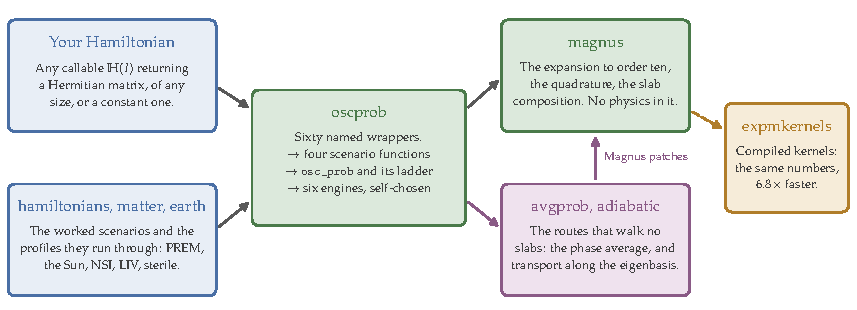
\includegraphics[width=0.98\textwidth]{architecture.pdf}
 \caption{\label{fig:architecture}The modules of \magnus\ and the path of a request through them. A Hamiltonian enters from the left, either supplied by the user as a function of position or built by {\tt hamiltonians} for one of the implemented scenarios, with the density profile provided by {\tt matter}, {\tt earth}, or {\tt solarmodels}. The request is handled in {\tt oscprob}, which contains the choice of engine of Section~\ref{sec:engines} and the refinement ladder of Section~\ref{sec:refinement}. From there the computation proceeds along one of two routes: through {\tt magnus}, which evaluates the expansion slab by slab and contains no physics, or through {\tt avgprob} and {\tt adiabatic}, which evaluate no slabs outside the non-adiabatic windows---the first for the phase average, the second for transport along the instantaneous eigenstates---and call {\tt magnus} back to compute the evolution across each window. The dashed arrow to {\tt expmkernels} indicates that this module affects only the speed: a {\tt NumPy} implementation of the same exponential exists behind it, and the test suite verifies that the two agree to round-off}
\end{figure*}
%%%%%%%%%%%%%%%%%%%%%%%%%%%%%%%%%%%%%%%%%%%%%%%%%%%%%

\smallskip

\textit{Errors and warnings that explain themselves.---}When a call is malformed, \magnus\ raises an error that says what is wrong and what it expected. For instance, requesting an Earth chord by its arrival direction but with the baseline set to {\tt None} raises an error explaining that the arrival direction sets the chord but the baseline may not be {\tt None}. A misspelled keyword raises one that names the closest valid keyword and lists the keywords the wrapper passes on to {\tt osc\_prob}. When a call is well formed but probably not what was meant, \magnus\ warns instead: \eg, when a baseline looks like it was given in kilometers rather than in eV$^{-1}$, or a density does not look like the unit it was declared in. And when the answer itself may be less accurate than requested, the warning says by how much, when it can, and what to change: \eg, how far outside the tolerance the refinement stopped, or that a discontinuity should be declared. 

%%%%%%%%%%%%%%%%%%%%%%%%%%%%%%%%%%%%%%%%%%%%%%%%%%%%%

\subsection{The \magnus\ architecture}
\label{sec:architecture}

Figure~\ref{fig:architecture} shows the modules of \magnus\ and the path of a request through them, from a Hamiltonian on the left to a probability on the right. A request arrives at the {\tt oscprob} module and leaves it either to {\tt magnus}, which evaluates the expansion slab by slab, to {\tt avgprob}, which computes the phase average of the probability, or to {\tt adiabatic}, which transports the neutrino state along the instantaneous eigenstates. The last two return to {\tt magnus} only to cross a non-adiabatic window with a Magnus patch. The route is selected internally by \magnus\ from the form of the request, not by the user; Section~\ref{sec:engines} gives the order in which the candidates are tried.

The numerical core is kept separate from the physics: {\tt magnus} imports nothing that concerns neutrinos, and its only dependency within the package is {\tt expmkernels}, the {\tt numba} compiled matrix exponential. The module is numerical linear algebra on an arbitrary matrix-valued function $\mathbb{A}(l)$, so it can be tested against the recursion of \equ{recursion} without involving any of the probability code. The physics, the environments, and the numerical core meet in one module, {\tt oscprob}, the only one that imports all three.

Table~\ref{tab:modules} lists the thirteen modules under {\tt src/magnus/}, together with the {\tt hamiltonians} subpackage, and the responsibility of each. The largest, {\tt oscprob}, holds all the wrappers; to avoid duplicating the same logic in each of them, its functions are organized in four layers, each calling the one below it.

%%%%%%%%%%%%%%%%%%%%%%%%%%%%%%%%%%%%%%%%%%%%%%%%%%%%%
\begin{figure*}[t!]
 \centering
 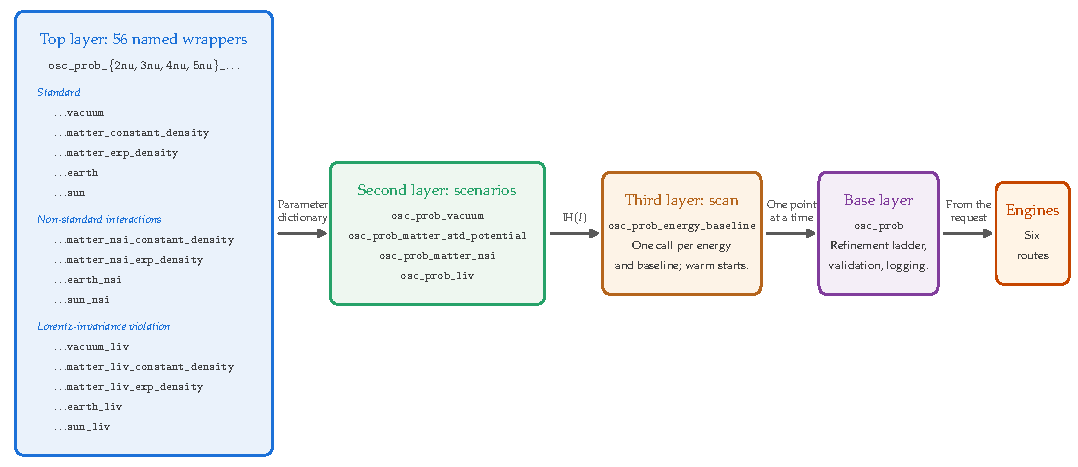
\includegraphics[width=\textwidth]{layers.pdf}
 \caption{\label{fig:layers}The four layers of {\tt oscprob}, and the engines each one tries. A request enters at one of the named wrappers, which convert their named arguments into a parameter dictionary and pass it to the scenario function of the second layer. That function builds the Hamiltonian and tries the first five engines of Section~\ref{sec:engines}, in order; if none applies, it passes the Hamiltonian to {\tt osc\_prob\_energy\_baseline}, which tries the cumulative scan over baselines and otherwise calls {\tt osc\_prob} once for every requested point. {\tt osc\_prob} is itself the seventh engine, the general Magnus ladder of Sec.~\ref{sec:refinement}. The wrappers are a product set: the fourteen environment-and-scenario names listed in the left box exist at each of the four flavor counts, giving $4 \times 14 = 56$ in all. There is no wrapper for non-standard interactions in vacuum, since those interactions require matter.}
\end{figure*}
%%%%%%%%%%%%%%%%%%%%%%%%%%%%%%%%%%%%%%%%%%%%%%%%%%%%%

Figure~\ref{fig:layers} shows the four layers:
\begin{enumerate}
\item The top layer consists of the named wrappers, such as {\tt osc\_prob\_3nu\_matter\_constant\_density} in Listing~\ref{lst:constant}. Each converts its named arguments into the parameter dictionary expected by the second layer and calls the function there for its scenario.
%%%%
\smallskip
%%%%
\item The second layer consists of four functions, one for each pre-defined physics scenario shipped with \magnus\ and each applicable to any number of flavors: {\tt osc\_prob\_vacuum}, {\tt osc\us prob\us matter\us std\us potential}, {\tt osc\_prob\_matter\_nsi}, and {\tt osc\_prob\_liv}. Each builds the Hamiltonian for its scenario and tries, in order, the engines that exploit its structure: the phase average, the adiabatic transport with Magnus patches, the interaction-picture expansion, the constant-Hamiltonian engine, and the energy-batched scan. If none of them applies, it passes the Hamiltonian to the third layer.
%%%%
\smallskip
%%%%
\item The third layer is {\tt osc\us prob\us energy\us baseline}, which receives the Hamiltonian together with the arrays of energies and baselines. It tries the cumulative scan over baselines; if that does not apply, it calls the base layer once for each point, seeding the refinement of each from the converged slab count of the previous one.
%%%%
\smallskip
%%%%
\item The base layer is {\tt osc\_prob}, the general Magnus ladder of Table~\ref{tab:engines}: it computes one probability matrix with the refinement ladder, and it is reached only when no engine above it applies. It can also be called directly with an arbitrary Hamiltonian, as in Listing~\ref{lst:constant}.
\end{enumerate}

The refinement keywords ({\tt n\_slabs}, {\tt max\us n\us slabs}, {\tt t\_breakpoints}, {\tt magnus\_exp\_order}, {\tt integration\us method}, {\tt rtol}, {\tt atol}, {\tt strict\_convergence}, and {\tt n\_jobs}) are declared by {\tt osc\_prob} and by the layers between it and the wrappers, but not by the wrappers themselves, which receive them through {\tt **kwargs}. Therefore, they do not appear in the signature of a wrapper, and {\tt help()} on a wrapper does not list them; its docstring names them and refers to {\tt osc\_prob}, where they are documented.

Extending \magnus\ usually requires only a new Hamiltonian. {\tt osc\_prob} accepts any function that returns a Hermitian matrix and does not depend on how that matrix was constructed, so a new term can be added to the array returned by an existing builder and the result passed on unchanged; Section~\ref{sec:building_new_hamiltonian} shows how. A new function in the second layer is needed only for physics that fits none of the four existing scenarios; the documentation\ \cite{MagnusDocs} shows how to write one, and why the shipped scenario functions are faster than a new one unless it dispatches to the same engines.

%%%%%%%%%%%%%%%%%%%%%%%%%%%%%%%%%%%%%%%%%%%%%%%%%%%%%
{\def\arraystretch{1.2}
\begin{table}[b!]
 {\small
 \begin{tabular}{@{}lp{6.1cm}@{}}
 Module & Responsibility \\
 \hline
 {\tt magnus} & Magnus expansion: collocation integrators, cumulative quadrature, slab composition, the unitary exponential \\
 {\tt expmkernels} & Compiled kernels for the exponential: Cayley-Hamilton at $2\times2$ and $3\times3$, batched Jacobi solver at $4\times4$ and $5\times5$ \\
 {\tt expansionterms} & Recursion of \equ{recursion}, in exact rational arithmetic, at any order \\
 {\tt adiabatic} & Adiabatic transport, detection of level crossings, the combined propagator \\
 {\tt avgprob} & Averaged probability \\
 {\tt earth} & PREM profile, geometry \\
 {\tt solarmodels} & Tabulated standard solar models: electron density and composition along a radial ray \\
 {\tt matter} & Density profiles, $V_{\rm CC}$, matter-potential projector \\
 {\tt hamiltonians} & Mixing matrices and the vacuum, matter, NSI, and LIV Hamiltonians \\
 {\tt globaldefs} & Constants, unit conversions, NuFIT sets \\
 {\tt oscprobstd} & Closed-form standard probabilities (validation) \\
 {\tt oscprob} & User-facing probability functions \\
 {\tt plotting} & Pre-packaged figure scripts \\
 {\tt cli} & The {\tt magnus} console script \\
 \end{tabular}}
 \caption{\label{tab:modules}The modules of \magnus\ v1.1.1. {\tt magnus} and {\tt hamiltonians} can be used and tested independently of the probability functions.}
\end{table}}
%%%%%%%%%%%%%%%%%%%%%%%%%%%%%%%%%%%%%%%%%%%%%%%%%%%%%

%%%%%%%%%%%%%%%%%%%%%%%%%%%%%%%%%%%%%%%%%%%%%%%%%%%%%

\subsection{Example: one request, through the layers}
\label{sec:one_request}

Listing~\ref{lst:layers} follows one request through the four layers of \figu{layers}. Its first block is the whole of what a user sends to \magnus: a call to the wrapper {\tt osc\_prob\_3nu\_earth} for a three-flavor probability at one energy along an Earth chord, with two refinement keywords. The blocks below it are not written by the user; they are the functions inside \magnus\ that the call passes through, in order. No specialized engine takes this request, so it descends all the way to {\tt osc\_prob}.

The wrapper computes the chord through the PREM (see \figu{prem}): the positions where it crosses the boundaries between layers, and the density along it. It collects the oscillation parameters it received by name into a dictionary, and calls the second-layer function for standard oscillations in matter, {\tt osc\_prob\_matter\_std\_potential}, with the flavor count, the density, the energy, the baseline, and the layer boundaries as breakpoints. That function converts the density to the potential $V_{\rm CC}$, builds the Hamiltonian of \equ{h_matter}, and tries the engines of Sec.~\ref{sec:engines} that can exploit its structure.

None of the engines 1--6 apply here: the declared breakpoints rule out the adiabatic transport, and a single energy rules out the energy-batched scan. Therefore, it passes the Hamiltonian to the third layer, {\tt osc\_prob\_energy\_baseline}, whose cumulative scan needs several baselines and does not apply either; it calls {\tt osc\_prob} once, for the one point, \ie, engine 7. Finally, {\tt osc\_prob} runs the refinement ladder of Sec.~\ref{sec:refinement}, with a slab edge on every layer boundary. The two refinement keywords in the request, {\tt rtol} and {\tt atol}, reach the scenario function through {\tt **kwargs}, and from there they are passed down explicitly, layer by layer, to {\tt osc\_prob}, which uses them.

\begin{lstlisting}[language=Python, caption={A request through the four layers of \figu{layers}: one energy along an Earth chord. The first block is what the user writes, the complete call. The four blocks below it are the functions inside \magnus\ that the call passes through, all defined in the module {\tt magnus.oscprob} ({\tt src/magnus/oscprob.py}) and abbreviated to the arguments that carry the request on.}, label={lst:layers}, float=tbp]
# ---- What the user writes: the whole request ----
# One energy, one chord, and two refinement keywords
P = osc_prob_3nu_earth(
        3.0*gd.UNIT_GEV, costhz=-0.5,
        L=chord(-0.5)*gd.UNIT_KM, **osc,
        rtol=1e-8, atol=1e-10)

# ---- Inside Magnus: what the call runs through ----
# Top layer: the named wrapper
def osc_prob_3nu_earth(energy, costhz, L,
        s12, s23, s13, dCP, D21, D31, ..., **kwargs):
    edges = earth.prem_layer_edges_along_chord(...)
    rho_func = ...   # PREM density along the chord
    return osc_prob_matter_std_potential(
        3, rho_func, energy, L,
        {'s12': s12, 's23': s23, 's13': s13,
         'dCP': dCP, 'D21': D21, 'D31': D31},
        t_breakpoints=edges, ..., **kwargs)

# Second layer: builds H, tries its engines
def osc_prob_matter_std_potential(num_flavors,
        rho_func, energy, L, osc_params,
        rtol, atol, ..., **kwargs):
    htot = ...   # Vacuum term + V_CC(l) * P
    ...          # Engines 1-5: none applies here
    return osc_prob_energy_baseline(htot, energy,
        L, rtol=rtol, atol=atol, ..., **kwargs)

# Third layer: the scan over (energy, baseline)
def osc_prob_energy_baseline(H_func, energy, L,
        rtol, atol, ..., **kwargs):
    ...          # Engine 6: one baseline, no
    return osc_prob(H_at_energy, L0, L,
                    rtol=rtol, atol=atol, ...)

# Base layer: the refinement ladder, one point
def osc_prob(H_func, l0, l1, rtol, atol, ...):
    ...          # Engine 7; rtol, atol used here
\end{lstlisting}

%%%%%%%%%%%%%%%%%%%%%%%%%%%%%%%%%%%%%%%%%%%%%%%%%%%%%

\subsection{The seven engines}
\label{sec:engines}

When a user requests a probability from \magnus, they do not need to select a method to compute it. Behind the interface of Sec.~\ref{sec:scope_interface}, the seven engines of \figu{layers} can answer the request. They are tried in a fixed order, from the most specialized to the most general, and the first one whose conditions the request meets answers it. An engine whose conditions are not met declines, and the request passes to the next one. The general Magnus ladder, which comes last, accepts every request.

\smallskip

\textit{How a request is assigned to an engine.}---No argument passed to a probability function names the engine explicitly; the content of the request decides. A request with {\tt average=True} goes to the averaged-probability engine. A Hamiltonian that does not vary along the path goes to the constant-Hamiltonian engine, at any number of energies and baselines. For a Hamiltonian that does vary, many energies at one baseline go to the energy-batched scan, and one energy at many baselines to the cumulative scan. A profile declared as exponential, at two flavors and one baseline, goes to the interaction picture. Every other request goes to the general Magnus ladder. Passing an array instead of looping over its entries can therefore change which engine computes the answer; Sec.~\ref{sec:cost} measures the difference in cost.

Not every entry point tries every engine. The matter scenario functions try the first five, in the order below; {\tt osc\_prob\_energy\_baseline} tries the cumulative scan; and {\tt osc\_prob} is the general ladder itself (Fig.~\ref{fig:layers}). {\tt osc\_prob\_vacuum} needs only the phase average and the constant engine. A Hamiltonian supplied by the user, through {\tt osc\_prob\_earth} or {\tt osc\_prob\_sun}, can reach the phase average, the adiabatic engine, the cumulative scan, and the ladder. A request for the evolution operator, {\tt return\_evolution\_operator=True}, goes to the ladder, the only engine that forms it.

One keyword, {\tt strategy}, controls the adiabatic engine only; it selects no other engine. Its default, {\tt 'auto'}, lets the adiabatic engine answer a request that meets its conditions, but only with an answer it can certify; otherwise the request passes on. Under {\tt 'auto'}, the engine also passes on two kinds of request that another engine answers faster: eight or more baselines at one energy, which the cumulative scan answers in one traversal, and a request at a loose tolerance ($\min(\epsilon_{\rm rel}, \epsilon_{\rm abs}) \geq 10^{-6}$) with a moderate accumulated phase (at most $10^4$), which the ladder answers at a tenth of the requested tolerance. {\tt 'hybrid'} makes the adiabatic engine answer whether or not it can certify, provided its other conditions hold. {\tt 'magnus'} excludes it. Therefore, the accuracy of the default is the accuracy of the certified answers; Sec.~\ref{sec:hybrid} reports it over the whole validation grid.

\smallskip

%%%%%%%%%%%%%%%%%%%%%%%%%%%%%%%%%%%%%%%%%%%%%%%%%%%%%
\begin{figure*}[t!]
 \centering
 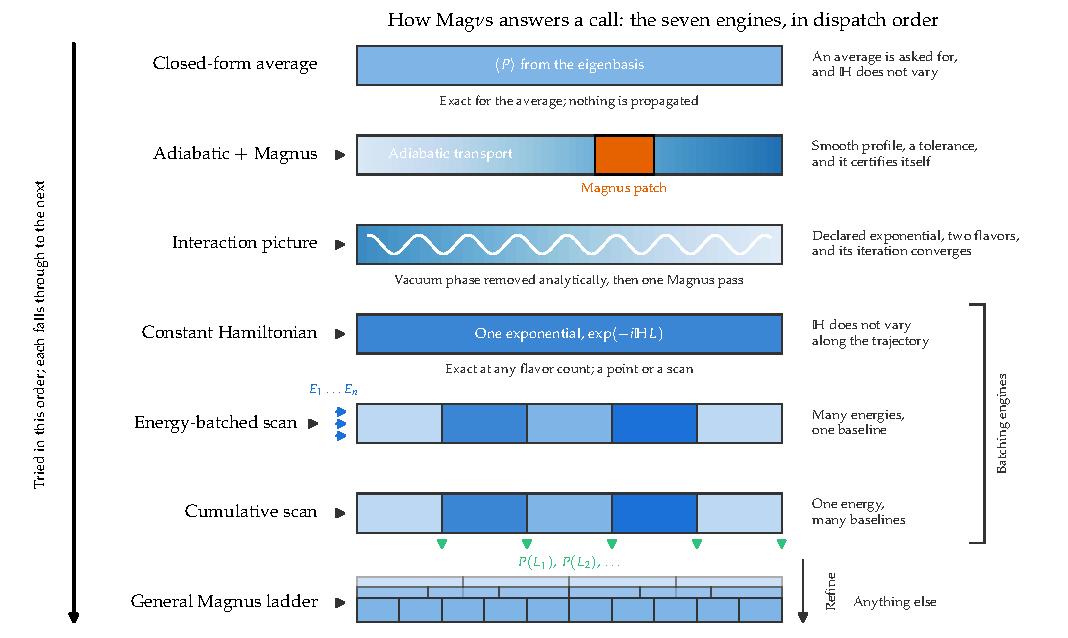
\includegraphics[width=\textwidth]{strategies.pdf}
 \caption{\label{fig:strategies}The seven engines of \magnus, in the order in which they are tried. A request that does not meet an engine's conditions, summarized on the right, passes to the next, so the general Magnus ladder answers whatever no other engine takes. Each row sketches what its engine does along the trajectory; shading represents the matter density. Averaged probability: the averaged probability from one eigenbasis in closed form; across declared discontinuities, the probability averaged over an energy window; or, where $\mathbb{H}$ varies smoothly, the average transported along the instantaneous eigenstates with a Magnus patch across each non-adiabatic crossing. Adiabatic $+$ Magnus: transport along the instantaneous eigenstates, with a Magnus patch across the resonance. Interaction picture: the vacuum phase removed analytically, leaving only the matter term to integrate over each slab. Constant Hamiltonian: a single exponential. Energy-batched scan: one set of slabs shared by every energy. Cumulative scan: one pass that records the probability at every requested baseline. General Magnus ladder: slabs refined until two successive levels agree. \tabl{engines} gives the conditions of each engine. See Sec.~\ref{sec:engines} for details.}
\end{figure*}
%%%%%%%%%%%%%%%%%%%%%%%%%%%%%%%%%%%%%%%%%%%%%%%%%%%%%

\textit{The engines.---}Figure~\ref{fig:strategies} and \tabl{engines} show the seven engines in the order in which \magnus\ tries them.
\begin{enumerate}
%%%%
\item \emph{Averaged probability.} This engine answers every request made with {\tt average=True}, by one of three routes chosen by $\mathbb{H}$. When $\mathbb{H}$ does not depend on position, it returns \equ{phase_average}, the probability with each interference term damped by the spread of its phase across the energy resolution. That is the quantity a solar or an astrophysical experiment measures. Where every phase has decohered, it is the limit \equ{averaged}. The engine diagonalizes $\mathbb{H}$ once at each energy and does not divide the path into slabs. When $\mathbb{H}$ varies smoothly along the path, the engine transports along the instantaneous eigenstates, keeping each phase with its weight, with the Magnus patch of Sec.~\ref{sec:hybrid} across every crossing that is not adiabatic. Without such a crossing, the result is \equ{averaged_varying}, for the initial state of Sec.~\ref{sec:average_keyword}. 

%%%%%%%%%%%%%%%%%%%%%%%%%%%%%%%%%%%%%%%%%%%%%%%%%%%%%
{\def\arraystretch{1.2}
\begin{table*}[t!]
 {\footnotesize
 \begin{tabular}{@{}p{3.3cm}p{3.3cm}p{10.6cm}@{}}
 Engine & Name in {\tt strategy\_info} & Condition \\
 \hline
 Averaged probability & {\tt 'average'} & An averaged probability is requested \\
 Adiabatic $+$ Magnus & {\tt 'hybrid'} & A smooth profile, a requested tolerance, no declared breakpoints, and a certified answer; under {\tt 'auto'}, not a loose tolerance with a moderate phase, nor eight or more baselines at one energy \\
 Interaction picture & {\tt 'ip\_exp'} & A profile declared as exponential, at two flavors and one baseline, and a converged iteration \\
 Constant Hamiltonian & {\tt 'constant'} & $\mathbb{H}$ does not vary along the trajectory; any number of flavors, a single point or a scan \\
 Energy-batched scan & {\tt 'separable'} & Many energies at one baseline \\
 Cumulative scan & {\tt 'cumulative'} & Many baselines at one energy \\
 General Magnus ladder & {\tt 'magnus'} & Every other request \\
 \end{tabular}}
 \caption{\label{tab:engines}The seven engines, in the order in which they are tried, with the name each reports through {\tt strategy\_info}. A request that fails the condition of a row passes to the next row, so the last is reached whenever no other applies. Since two neighboring engines are different methods, the accuracy can change in a step at the boundary between them, in either direction; Section~\ref{sec:implementation_limits} treats these boundaries.}
\end{table*}}
%%%%%%%%%%%%%%%%%%%%%%%%%%%%%%%%%%%%%%%%%%%%%%%%%%%%%

When the profile has discontinuities, declared through {\tt t\_breakpoints} or {\tt t\_slab\_edges} (as for the layers of the Earth), $\mathbb{H}$ has no instantaneous eigenstates to transport along. The engine then computes the probability at several energies across a window around the requested one and returns their mean. That mean depends on the width of the window, so it is not the limit returned by the other two routes, and \magnus\ warns whenever it uses this route (Secs.~\ref{sec:average_keyword} and \ref{sec:shock}). Section~\ref{sec:astro} uses this engine for astrophysical neutrinos.
%%%%
\smallskip
%%%%
\item \emph{Adiabatic $+$ Magnus.} This engine is the adiabatic transport with Magnus patches of Sec.~\ref{sec:hybrid}. It applies to any Hamiltonian that varies smoothly along the trajectory, at any number of flavors, whether built by a scenario function or supplied by the user. It is the engine for a large accumulated phase: its cost is set by the grid on which $\mathbb{H}$ is diagonalized and by the crossings it patches, not by the phase, which the general ladder would have to resolve slab by slab. It declines when slab edges or breakpoints are supplied, when no tolerance is requested, or when $\mathbb{H}$ is not resolved on the grid on which it searches for crossings; under {\tt strategy='auto'}, it also declines when its certification fails and in the two cases described above.
%%%%
\smallskip
%%%%
\item \emph{Interaction picture.} At low energy, the vacuum phase is large, and a slab method must resolve every cycle of it, although that part of the evolution is known exactly. Switching to the interaction picture removes this phase. The switch applies to any Hamiltonian that separates into a position-independent part and a position-dependent term of the form $V(l)\,\mathbb{M}$, with $\mathbb{M}$ a fixed matrix: the position-independent part is diagonalized once at each energy, its evolution is factored out analytically, and only the envelope $V(l)$ remains to be integrated. In \magnus, the position-dependent term is the matter term, so the Hamiltonian is $\mathbb{H}(E, l) = \mathbb{H}_0(E) + V_{\rm CC}(l)\,\mathbb{P}$. Here $\mathbb{P}$ is the matter projector (Sec.~\ref{sec:recap}), plus the non-standard-interaction matrix if present, and $\mathbb{H}_0$ collects the vacuum term and, if present, the Lorentz-violating term.

The engine is specific to an exponential envelope, $V_{\rm CC}(l_0 + s) = V_{\rm CC}(l_0)\,e^{-s/l_{\rm scale}}$. The first-order Magnus term needs the integral of the envelope against the vacuum phase, and for an exponential envelope that integral has a closed form. For any other envelope it would have to be computed by quadrature, which would again have to resolve the vacuum phase. The solar density falls close to exponentially over most of the radius, and solar neutrinos, with their large vacuum phase, are the case the engine is for. Over a slab of length $h$ starting at $l_0$, the first-order term is
\begin{equation}
 \label{equ:ip_omega1}
 \big(\tilde{\Omega}_1\big)_{jk}(h)
 = -i\, \big(\tilde{\mathbb{P}}\big)_{jk}\, V_{\rm CC}(l_0)\,
 \frac{e^{(i \Delta_{jk} - 1/l_{\rm scale})h} - 1}{i \Delta_{jk} - 1/l_{\rm scale}} ,
\end{equation}
where a tilde marks a matrix in the eigenbasis of $\mathbb{H}_0$, $\Delta_{jk} = \lambda_j - \lambda_k$ is the gap between two of its eigenvalues, and $l_{\rm scale}$ is the scale height; the expression holds for $j = k$ as well. Equation~(\ref{equ:ip_omega1}) integrates the exponential envelope exactly over the slab: $V_{\rm CC}(l)$ is not replaced by a constant or a straight line within the slab, as a quadrature would do. The only approximation is the truncation of the series at first order. It is accurate wherever the matter term is a small perturbation on the vacuum splitting, and it improves as the energy falls, since $\Delta_{jk}$ grows as $1/E$. The engine doubles the number of slabs until two successive answers agree to the requested tolerance, twice in a row.

Four conditions have to hold for this engine to take a request: two flavors, a profile built with {\tt exp\_density\_profile} (the default of the solar wrappers; a tabulated solar model is not one), a single baseline, and no slab edges or breakpoints. Under {\tt strategy='auto'}, it is also skipped when the adiabatic engine hands the request to the ladder. (The limit of two flavors is empirical: the neglected second-order term is about a thousand times larger at three flavors than at two, and the number of slabs needed to certify an answer is then too large for the engine to be fast.) At an MSW resonance, the matter term is no longer small, the answers stop agreeing before the engine reaches its limit on the number of slabs, and the request passes to the next engine.
%%%%
\smallskip
%%%%
\item \emph{Constant Hamiltonian.} When $\mathbb{H}$ does not vary along the trajectory, the Magnus series terminates at its first term: every $\Omega_k$ beyond $\Omega_1$ is a nested commutator of $\mathbb{H}$ with itself, hence zero. The evolution operator is therefore $\exp(-i\mathbb{H}L)$ exactly, with no discretization at all, and a whole scan over $n_E$ energies is one stacked exponential over an $(n_E, d, d)$ array, with $d$ the number of flavors. The engine applies at any number of flavors, to a single point as well as to a scan, and it accepts a different baseline for each point, which the energy-batched scan below does not. Refinement keywords are accepted and ignored, since they can only ask for a refinement of something already exact; a value that {\tt osc\_prob} would reject is declined, so that the user sees the same error as on any other route.
%%%%
\smallskip
%%%%
\item \emph{Energy-batched scan.} A scan over many energies at one baseline, computed point by point, traverses the same profile once per energy although the profile does not depend on it. When $\mathbb{H}$ separates as above (\eg, as the standard, non-standard-interaction, and Lorentz-violating Hamiltonians do), this engine samples the potential once per refinement level and shares it across the batch; the quadrature, the commutators, the exponentials, and the slab products carry the energy as a batch dimension, and energies that have converged drop out of further refinement.
%%%%
\smallskip
%%%%
\item \emph{Cumulative scan.} The complementary case is one energy at many baselines, $L_1 < L_2 < \dots < L_N$. The path to each baseline contains the path to the previous one, $\mathbb{U}(0, L_2) = \mathbb{U}(L_1, L_2)\,\mathbb{U}(0, L_1)$, so this engine traverses the profile once and records the running product at each of the $N$ baselines, where computing them independently would traverse it $N$ times. The traversal is chunked and each recorded product is converted to a probability at once, so that peak memory scales with the chunk and not with the number of baselines.
%%%%
\smallskip
%%%%
\item \emph{General Magnus ladder.} The last engine is the refinement ladder of Sec.~\ref{sec:refinement}. It assumes only a Hermitian $\mathbb{H}(l)$: it lays slabs along the trajectory, builds the Magnus expansion on each, composes them in order, and raises the slab count until the probabilities computed in two successive stages agree to the requested tolerance. It is reached whenever no engine above it applies.
\end{enumerate}

Comparing the answers of two engines is a useful test of accuracy when the engines use different methods, \eg, the adiabatic engine and the general ladder. It is a weak test when they use the same method: the general ladder, the cumulative scan, and the energy-batched scan all apply the Magnus expansion on slabs, so they tend to err in the same way. A user who doubts a result can test with {\tt cross\_check\_strategies}: it takes the same arguments as the function being checked, computes the request with every engine that applies to it, and reports how far apart the answers are. It is not run by default, since it raises the cost of a call. That said, no engine can see a feature narrower than the grid on which it samples the profile, so all of them can agree and be wrong together; for that, the reference has to come from outside \magnus\ (Sec.~\ref{sec:validation}).

\smallskip

\textit{Seeing which engine answered.}---When an engine declines a request and the next one takes it, the user is usually not told (the exception is the adiabatic engine declining a profile with a jump or a feature too narrow for its sampling grid, which is warned about once per session). This happens on ordinary calls, where a warning each time would be noise. Instead, the user can ask which engine answered once the probability is returned. A dictionary passed as {\tt strategy\_info} to the probability function returns with, among other entries, the engine that answered ({\tt engine}); whether, if it was the adiabatic engine, the answer was certified ({\tt certified}); and the engines that attempted the request and gave up, each with its reason ({\tt declined}). The keyword is accepted by every scenario function and every wrapper, and by {\tt osc\_prob\_earth} and {\tt osc\_prob\_sun}. This makes an answer traceable. A result that moves when a point is added to a scan, or a call that suddenly costs more, is often a change of engine, and the dictionary names it.

%%%%%%%%%%%%%%%%%%%%%%%%%%%%%%%%%%%%%%%%%%%%%%%%%%%%%

\subsection{Batching and parallelization}
\label{sec:batching}

In \magnus, a request for many probabilities can be made faster in two ways, batching and parallelization, which act differently and mostly do not combine.

\begin{itemize}
\item \emph{Batching} means passing an array in one call: many energies at one baseline, or many baselines at one energy. A call can also take equal-length arrays of energies and baselines, which it pairs point by point: the first energy with the first baseline, and so on. These points are computed one at a time, unless $\mathbb{H}$ does not vary along the path. To get the probability at every energy for each of several baselines, the user makes one call per baseline, each with the full array of energies.

A request with one shared value can reach one of the batched engines of Sec.~\ref{sec:engines}, which reuse work across the array. The \textit{energy-batched scan} samples the profile once per refinement level and carries the energy as a batch dimension through every slab; the \textit{cumulative scan} traverses the profile once and records the running product at every requested baseline. Both run in a single process (any use of further cores comes from the linear-algebra library under {\tt NumPy}, not from \magnus). The gain is that the profile is not traversed once per point. Where $\mathbb{H}$ does not vary, the batched answers are identical, bit for bit, to those computed one point at a time. Where it varies, both answers meet the requested tolerance but are not identical, since each refines its grid on its own; with the grid fixed, they agree to $10^{-12}$ (Sec.~\ref{sec:validation}).
%%%%
\item \emph{Parallelization} means computing points in several processes at once, on several cores, as specified by the {\tt n\_jobs} argument. \magnus\ uses the {\tt joblib} library for it: the first point is computed in the calling process, {\tt n\_jobs} processes are started, and the remaining points are divided among them, each computed on the per-point path. The gain is bounded by the number of cores and by the cost of moving work between them. Since every point starts its refinement from the first point rather than from its neighbor, a parallel scan agrees with a serial one to the requested tolerance, not bit for bit (Sec.~\ref{sec:cost}).

The gain is well below the number of parallel processes. Section~\ref{sec:cost} measures it on an Earth chord where every energy has its own baseline, so that no batched engine applies. On a machine with ten cores (Sec.~\ref{sec:timing_protocol}), ten processes complete a scan of 1\,000 energies 1.9 times as fast as one process does, a scan of 5\,000 energies 2.5 times as fast, and a scan of 20\,000 energies 2.8 times as fast: the gain grows with the size of the scan and stays far from 10.
\end{itemize}

%%%%%%%%%%%%%%%%%%%%%%%%%%%%%%%%%%%%%%%%%%%%%%%%%%%%%
\begin{figure}[t!]
 \centering
 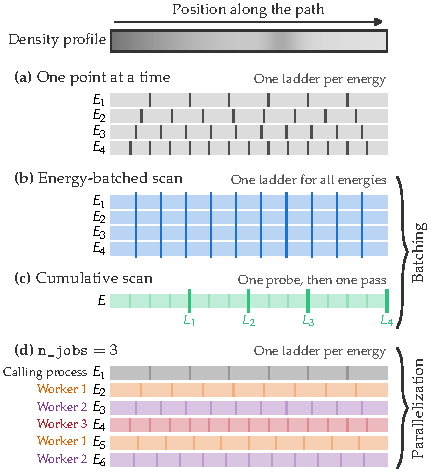
\includegraphics[width=\columnwidth]{batching.pdf}
 \caption{\label{fig:batching}Four ways \magnus\ computes a scan, drawn along one density profile (shading). Each bar is the final slab grid of one refinement ladder, which traverses the profile once per level; its color marks the process that runs it. (a) One point at a time. (b) The energy-batched scan, with one grid shared by every energy. (c) The cumulative scan, at one energy, recording the probability at every requested baseline ($L_1$ to $L_4$) in one pass. (d) Parallelization with {\tt n\_jobs} $= 3$: the first point runs in the calling process and the rest are shared out among three workers. See Sec.~\ref{sec:batching} for details.}
\end{figure}
%%%%%%%%%%%%%%%%%%%%%%%%%%%%%%%%%%%%%%%%%%%%%%%%%%%%%

Figure~\ref{fig:batching} shows why the two differ. Computed one point at a time, a scan of $N$ energies runs $N$ refinement ladders. Batching removes most of that work: the energy-batched scan runs one ladder for all $N$ energies, sampling the profile once per slab, and the cumulative scan covers every baseline in a single pass. Parallelization does not reduce the work: all $N$ ladders still run, but several at a time, on different cores. At best, this divides the run time by the number of processes; in practice, the cost of starting the processes and moving work between them keeps the gain well below that.

Batching over energies and parallelization exclude each other. The energy-batched scan and the constant-Hamiltonian engine answer only at {\tt n\_jobs} $= 1$; any other value sends the scan to the per-point path, computed in parallel, which is slower than the batched path in one process. For a three-flavor scan of 5\,000 energies between 0.5 and 20~GeV along the PREM chord at $\cos\theta_z = -0.9$, with a baseline of 11\,468~km, the batched path takes 0.11~s in one process; ten processes take 1.1~s (Sec.~\ref{sec:cost}). The cumulative scan does not depend on {\tt n\_jobs}: a scan over baselines at one energy is answered in one process regardless.

In practice, for the majority of applications of \magnus, the user should pass arrays and leave {\tt n\_jobs} at its default of 1. Setting {\tt n\_jobs} above 1 pays only for a scan that no batched engine accepts, such as one where every energy has its own baseline; \figu{njobs_scaling} shows the gain in that case.

%%%%%%%%%%%%%%%%%%%%%%%%%%%%%%%%%%%%%%%%%%%%%%%%%%%%%

\subsection{Declaring the structure of a profile}
\label{sec:declaring_edges}

Two keywords let the user place slab edges by hand. They serve similar, but different purposes:
\begin{itemize}
\item {\tt t\_breakpoints} names positions that must be slab edges. The ladder of Section~\ref{sec:refinement} keeps its own grid, inserts an edge at each named position at every refinement level, then refines as usual to the requested tolerance. It is meant for a profile with a density jump, a kink, or a front at a known position: the user states where the profile is not smooth, and the package chooses the resolution. A tabulated profile, for instance, has a kink at every row of the table (the solar tables are interpolated linearly in the logarithm of the density), and the rows are where to declare breakpoints.

Declaring breakpoints also changes which engine answers. It excludes the adiabatic engine of Sec.~\ref{sec:hybrid}, and with {\tt average=True} it switches to the average over an energy window, a different quantity (Sec.~\ref{sec:average_keyword}). On a scan over baselines, declaring a front is the cure for it, as Sec.~\ref{sec:shock} shows on the forward shock and contact discontinuity of a supernova ray. At a single point it is not always an improvement, since the general ladder may then be less accurate than the adiabatic engine would have been; \magnus\ says so when it detects an undeclared jump.
%%%%
\item {\tt t\_slab\_edges} gives the complete grid of positions at which the evolution operator is evaluated, as a list of $[{\rm start}, {\rm end}]$ pairs, one per slab. It replaces the grid of the refinement ladder, so the slabs are fixed and are never refined. It is meant for a grid that can be justified in full, with no tolerance requested, so that the call is a single evaluation of the expansion on that grid. The user then takes over responsibility for the accuracy: nothing moves or adds an edge. If a tolerance is requested anyway, the ladder has nothing to refine at the default quadrature, repeats the same evaluation, and warns that the tolerance was not achieved. {\tt t\_breakpoints} is ignored when {\tt t\_slab\_edges} is given.

This keyword is intended for piecewise-constant profiles, such as the castle wall of \figu{arrangement}. With one slab per constant piece, the result is exact, because the Hamiltonian is constant within each slab and the Magnus expansion terminates at its first term. For every other profile, {\tt t\_breakpoints} is the keyword to use.
\end{itemize}

%%%%%%%%%%%%%%%%%%%%%%%%%%%%%%%%%%%%%%%%%%%%%%%%%%%%%
\begin{figure}[t!]
 \centering
 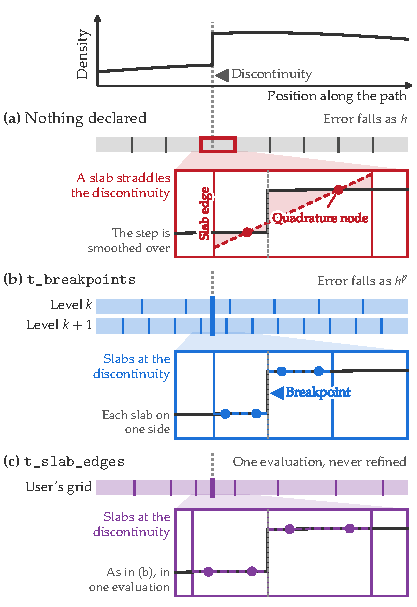
\includegraphics[width=\columnwidth]{declaring_edges.pdf}
 \caption{\label{fig:declaring_edges}What a density discontinuity does to a slab, and the two ways of declaring it. \textit{Top:} a density profile with one discontinuity. Each enlargement shows the same stretch of the path around the discontinuity: the true density, the slab edges, the two quadrature nodes of each slab, and the straight line through the values of $\mathbb{H}$ at those nodes, which is how the quadrature sees $\mathbb{H}$ within the slab; the shaded area is the difference between what the quadrature sees and the true density. \textit{(a)} Nothing declared: on the refinement ladder's uniform grid, one slab straddles the discontinuity, and the step is smoothed over. Refining narrows that slab but never removes it, so the error falls only roughly in proportion to the slab width. \textit{(b)} {\tt t\_breakpoints}: the grid changes from one refinement level to the next, but an edge, the breakpoint, stays at the discontinuity; every slab lies on one side of it, and the error falls as $h^p$. \textit{(c)} {\tt t\_slab\_edges}: the user's grid is evaluated once and its slabs are never refined. With an edge at the discontinuity, every slab lies on one side of it, as in (b); a grid that misses a discontinuity is left as it is. See Sec.~\ref{sec:declaring_edges} for details.}
\end{figure}
%%%%%%%%%%%%%%%%%%%%%%%%%%%%%%%%%%%%%%%%%%%%%%%%%%%%%

Figure~\ref{fig:declaring_edges} shows why a discontinuity must be declared. Refinement cannot fix a slab that straddles a discontinuity, so a higher order gains nothing. An edge placed at the discontinuity restores the order. {\tt t\_breakpoints} keeps that edge while the ladder refines the rest of the grid. {\tt t\_slab\_edges} fixes the whole grid, with no refinement, so it is only as good as the edges the user gives.

The most common case, a neutrino crossing the Earth, needs no action from the user. PREM describes the Earth as concentric layers: the density varies smoothly inside each layer and jumps at the boundaries between them. The Earth wrappers pass the positions where a trajectory crosses a boundary through {\tt t\_breakpoints} themselves. A core-crossing trajectory ($\cos\theta_z = -0.9$) crosses 16 boundaries. With slabs of equal width, the error stops falling: at orders 2, 4, and 6 alike, it stays between $10^{-3}$ and $10^{-5}$ even with 2\,000 slabs. With an edge at each crossing, the error falls as $h^p$ at every order, so the orders differ only in cost: at 5~GeV, an error of $10^{-8}$ takes about 2\,000 slabs at order 2, 64 at order 4, and 16 at order 6. Over 150 random piecewise-constant profiles, declaring the jumps lowers the median error from about $10^{-3}$ to $10^{-12}$.

Listing~\ref{lst:edges} shows the use of {\tt t\_breakpoints} and {\tt t\_slab\_edges} on the castle-wall profile of \figu{arrangement}. Declaring the 23 density jumps through {\tt t\_breakpoints} gives the exact answer at the first level at which two stages agree, on the grid of the ladder with the jumps added as edges. Giving the 24 slabs through {\tt t\_slab\_edges} gives the same answer in a single evaluation, since the profile is constant within every slab. A grid of twelve slabs, each straddling one jump, is off by about $10^{-3}$; nothing in the package repairs it, because the user owns that grid. Section~\ref{sec:prem} declares the boundaries of PREM, and Sec.~\ref{sec:shock} declares a shock front the same way.

%%%%%%%%%%%%%%%%%%%%%%%%%%%%%%%%%%%%%%%%%%%%%%%%%%%%%
\begin{lstlisting}[language=Python, caption={The two ways of placing slab edges by hand, on the castle-wall profile of \figu{arrangement}. {\tt t\_breakpoints} adds the positions of the jumps to the grid of the refinement ladder, which then refines as usual. {\tt t\_slab\_edges} replaces the grid with the given {[}start, end{]} pairs, which stay fixed. The first two calls return the exact result, because the profile is constant within every slab. The third call passes a grid whose slabs straddle the jumps: its result is off by $6 \cdot 10^{-4}$, and nothing corrects it, because the grid is the user's. Section~\ref{sec:shock} declares the two fronts of a supernova shock through {\tt t\_breakpoints} in the same way.}, label={lst:edges}, float=tbp]
import numpy as np
import magnus.oscprob as oscprob
import magnus.globaldefs as gd

osc = gd.load_nufit_params('NuFIT 6.1')
E, L = 2.0*gd.UNIT_GEV, 6000.0*gd.UNIT_KM
# 24 slabs of 250 km, alternating 2 and 8 g/cm^3
edges = np.linspace(0.0, L, 25)
rho = np.where(np.arange(24) % 2 == 0, 2.0, 8.0)

def castle_wall(l):
    k = np.searchsorted(edges, l, side='right') - 1
    return rho[np.clip(k, 0, 23)]

kw = dict(nu_i=gd.NUMU, nu_f=gd.NUE,
          density_matter_is_in_g_per_cm3=True)
prob = oscprob.osc_prob_matter_std_potential

# The jumps declared: the ladder keeps its own grid,
# adds an edge at each of the 23 jumps, then refines
# to the tolerance
P1 = prob(3, castle_wall, E, L, osc,
          t_breakpoints=edges[1:-1],
          rtol=1.0e-8, atol=1.0e-10, **kw)

# The grid given in full, as [start, end] pairs: one
# slab per layer, no refinement, a single evaluation
pairs = np.column_stack([edges[:-1], edges[1:]])
P2 = prob(3, castle_wall, E, L, osc,
          t_slab_edges=pairs, rtol=None, atol=None,
          **kw)

# A grid of 12 slabs, each straddling one jump: the
# user owns this grid, and nothing repairs it
wide = np.column_stack([edges[:-1:2], edges[2::2]])
P3 = prob(3, castle_wall, E, L, osc,
          t_slab_edges=wide, rtol=None, atol=None,
          **kw)

# P1 = P2 = 0.0240046, exact: the profile is constant
# within every slab.  P3 = 0.0246158, off by 6e-4
\end{lstlisting}
%%%%%%%%%%%%%%%%%%%%%%%%%%%%%%%%%%%%%%%%%%%%%%%%%%%%%

%%%%%%%%%%%%%%%%%%%%%%%%%%%%%%%%%%%%%%%%%%%%%%%%%%%%%

\subsection{Documentation and executable examples}
\label{sec:documentation}

\magnus\ is documented at four levels, from overview to detail:
\begin{itemize}
\item \emph{The README} of the repository~\cite{Magnus}: installation, a quick start from Python and from the command line, an overview of what \magnus\ computes, and when it is the right tool.
\item \emph{The documentation site}\ \cite{MagnusDocs}, whose source is kept in the repository beside the code. It presents the method of Sec.~\ref{sec:method} in the form in which it is implemented: one page derives the expansion terms at any order; others cover the adiabatic transport with Magnus patches of Sec.~\ref{sec:hybrid}, the phase average of Sec.~\ref{sec:averaged}, and the engines of Sec.~\ref{sec:engines} with the order in which they are tried. A performance page lists every tuned constant with the set of cases on which it was measured, or states that it was not measured. A diagnostics page explains every warning \magnus\  raises.
\item \emph{The API reference}, part of the documentation site, generated from the docstrings of the source. It documents every public function, with its parameters, units, and examples.
\item \emph{The notebooks}: 29 executable notebooks, listed in \ref{app:notebooks}, work through these topics with examples. One of them, notebook \#28, produces every figure in this paper. A workflow executes all the notebooks whenever the package or the notebooks change in the repository.
\end{itemize}

%%%%%%%%%%%%%%%%%%%%%%%%%%%%%%%%%%%%%%%%%%%%%%%%%%%%%

\subsection{Installation}

The released version of \magnus\ is on the Python Package Index (PyPI)\ \cite{MagnusPyPI}. It is installed with
\begin{verbatim}
pip install magnuspy
\end{verbatim}
This command also installs every dependency \magnus\ needs; for most users, it is the whole installation. \magnus\ requires Python 3.10 or later; it has been tested with up to 3.13.

The PyPI package does not include the notebooks of \ref{app:notebooks} or the test suite of Sec.~\ref{sec:validation} and \ref{app:tests}. \ref{app:tests}. The notebooks have saved output and can be read in the repository~\cite{Magnus}. To run or modify them, the user clones the repository:
\begin{verbatim}
git clone https://github.com/mbustama/Magnus.git
\end{verbatim}
The notebooks are in the {\tt notebooks} folder. From the clone, \magnus\ can also be installed directly, which gives access to changes not yet released on PyPI:
\begin{verbatim}
cd Magnus
# The package:
pip install -e .                 
# Plus what the notebooks need:
pip install -e ".[notebooks]"    
# Plus what the tests need:
pip install -e ".[test]"         
\end{verbatim}
Opening the notebooks interactively also requires a Jupyter front end, such as JupyterLab. Only users who contribute to \magnus\ typically need to run the test suite.

Installing \magnus\ in a dedicated virtual environment ({\tt conda} or {\tt venv}) is supported, but not required.

%%%%%%%%%%%%%%%%%%%%%%%%%%%%%%%%%%%%%%%%%%%%%%%%%%%%%

\subsection{Code availability}

We develop \magnus\ in the public GitHub repository\ \cite{Magnus}, which holds the source, the test suite, the notebooks, the documentation source, this paper, release notes, and the change log. This paper describes version 1.1.1. We release \magnus\ under the GNU General Public License v3.0. 

%%%%%%%%%%%%%%%%%%%%%%%%%%%%%%%%%%%%%%%%%%%%%%%%%%%%%

\subsection{Code validation}
\label{sec:validation}

The repository carries about 1\,600 tests, run on Python 3.10 through 3.13, covering 93\% of the statements and branches of the code. \ref{app:tests} groups the tests by what they cover. The validation is layered, and the layers are independent on purpose.

\subsubsection{Against the derivation}

We compare every expansion term the code evaluates, $\Omega_1$ to $\Omega_{10}$, against terms generated independently from the recursion of \ref{app:terms}, on a Hamiltonian chosen so that no term vanishes identically. The two agree to a relative $10^{-11}$ at every order, the round-off of the quadrature that evaluates them.

\subsubsection{Against closed forms}

Two- and three-flavor vacuum oscillations, and two-flavor constant-density matter oscillations, for neutrinos and antineutrinos, agree with their analytic expressions to $10^{-12}$.

\subsubsection{Against an independent solver}

The reference is a {\tt DOP853} integration of the evolution equation (order-8 Runge-Kutta\ \cite{Prince:1981dop}) at ${\tt rtol} = 10^{-12}$ and ${\tt atol} = 10^{-14}$. Where a test quotes an error close to the accuracy of the reference, the reference is itself checked by tightening {\tt rtol} to $10^{-13}$. For a constant Hamiltonian, or a piecewise-constant one whose edges are declared, {\tt scipy.linalg.expm} is exact and is used instead. On a model Hamiltonian, halving the slab width divides the error by about 4, 16, and 64 at orders 2, 4, and 6 on the default collocation path: the factor $2^{p}$ expected when the global convergence rate equals the requested order (Sec.~\ref{sec:order_is_the_slab_product}).

\subsubsection{Against itself, where meaningful}

Repeated calls, and a scan over baselines given in any order, are asserted to return identical results, bit for bit, so an optimization that changes an answer fails rather than passing quietly. A parallel run is held to the requested tolerance against a serial one, not to bit identity, since each worker starts its refinement from the first point rather than from its neighbor. The energy-batched scan is held to $10^{-12}$ against the per-point path, with the grid and the tolerances pinned so that the two are arithmetically the same problem; left to refine on its own, it agrees with the per-point path to within the requested tolerance. No Magnus path is ever scored against another as an accuracy measurement: a cross-check between two paths is reported as agreement, never as accuracy.

\subsubsection{Against a population}

Some tests do not check one case at a time. Each draws a set of random density profiles, computes the probability along every one at a requested tolerance of $10^{-3}$, compares each answer with the reference, and then judges the errors as a set: their median, their worst value, and how many are \emph{silent misses}. A silent miss is an answer outside the requested tolerance that carries no warning of any kind. It is the failure that matters: an inaccurate answer with a warning has been caught by the package; a silent one has not. The test passes or fails on these numbers, not on any single profile, because a random profile can always be found on which a method does poorly, whereas a regression in the code shifts the whole set. Two populations run with the test suite. Over 40 random smooth profiles at two and three flavors, the median error is about $10^{-8}$, with one silent miss, 8\% above the tolerance. Over 120 random piecewise-constant profiles at two to five flavors, with the edges deliberately left undeclared, 19 answers fall outside the tolerance, and every one of them comes with a warning.

Larger batteries, run by hand rather than with every test, measured the same quantities on more cases. Over 145 random smooth profiles, the median error was about $6 \cdot 10^{-8}$, with about 4\% silent misses, each within a factor of three of the tolerance. Over 150 random piecewise-constant profiles with their edges declared, the median error was about $10^{-12}$, with no silent miss. Over 164 Earth, solar, vacuum, and constant-density configurations, there was no silent miss.

\subsubsection{Continuous integration}

Every push to the repository runs the above tests on the four supported Python versions, a linter, and a build of the documentation that treats every warning as an error. The notebooks are executed whenever the package or the notebooks change. Before each release, the tests run once more against a regular installation of the package, as a user would have it, and the files uploaded to PyPI are checked for valid metadata.

%%%%%%%%%%%%%%%%%%%%%%%%%%%%%%%%%%%%%%%%%%%%%%%%%%%%%

\subsection{Limitations}
\label{sec:limitations}

The limitations of \magnus\ are of two kinds. Those of the method follow from what every engine assumes: a Hermitian Hamiltonian, fixed before the propagation and sampled on a grid of positions; no implementation would remove them. Those of the implementation follow from choices made in the code, and a later version could remove them.

%%%%%%%%%%%%%%%%%%%%%%%%%%%%%%%%%%%%%%%%%%%%%%%%%%%%%

\subsubsection{Limitations of the method}

\textit{Open systems.}---\magnus\ solves the Schr\"odinger equation for a Hermitian Hamiltonian. Every truncation of the Magnus expansion is anti-Hermitian, so the evolution it produces is unitary at every order; this is the property the method rests on. Decoherence, coupling to a bath, and neutrino decay to invisible states remove probability from the system or damp the coherence between mass eigenstates. They are described by a density matrix that obeys a non-unitary evolution equation, or by a Hamiltonian with an anti-Hermitian term, neither of which the method admits. {\tt nuSQuIDS}\ \cite{Delgado:2014kpa, NuSQuIDS} is the tool for those problems.

\smallskip

\textit{Collective oscillations.}---In a dense neutrino gas, the Hamiltonian depends on the flavor content of the neutrinos\ \cite{Duan:2010bg, Mirizzi:2015eza}, so the problem is nonlinear and has to be solved self-consistently. In \magnus, the Hamiltonian is fixed before the propagation begins, whether built by the package or supplied by the user, and it does not change with the neutrino state. A self-consistent solution would need an outer iteration that updates $\mathbb{H}$ from the solution and propagates again; \magnus\ could serve as the propagator inside such an iteration, but it does not ship with one.

\smallskip

\textit{A feature narrower than every grid.}---Every engine in \magnus\ samples the Hamiltonian on a grid of positions. A feature narrower than the finest of those grids falls between the samples, so all the engines miss it together, and a cross-check between them cannot detect the error. We measured this on a Gaussian resonance whose width is $10^{-5}$ of the trajectory: every engine returned an answer wrong by about $10^{-2}$ against a requested tolerance of $10^{-3}$. To catch such features, the scenario functions for standard matter and for non-standard interactions also scan the density profile itself. When the scan finds variation concentrated between grid points, it warns and names the breakpoints to declare. It catches most such features, but not all. A breakpoint at the feature, declared by the user or taken from the warning, brings the same case to $10^{-4}$. This limitation belongs to every method that samples the Hamiltonian on a grid.

%%%%%%%%%%%%%%%%%%%%%%%%%%%%%%%%%%%%%%%%%%%%%%%%%%%%%

\subsubsection{Limitations of the implementation}
\label{sec:implementation_limits}

\textit{A constant Hamiltonian.}---When the Hamiltonian does not depend on position, the evolution operator is a single exponential, which \magnus\ evaluates in closed form (Sec.~\ref{sec:exponential}), to round-off. The cost is set by the implementation, not by the problem: the exponential comes wrapped in the dispatch and validation of a general solver, which have nothing to do here. A code built for the constant case alone is therefore cheaper, by about a hundred times per point against the three-flavor specialization {\tt NuFast-LBL}~\cite{Denton:2024pzc} (Sec.~\ref{sec:comparison}).

\smallskip

\textit{Density fluctuations at every scale.}---The profile scan described above looks for variation concentrated in one place, so it cannot see variation spread evenly over every scale. We tested this on Kolmogorov density fluctuations of the kind used in supernova studies\ \cite{Loreti:1995ae, Patton:2013dba, Patton:2014lza}, with a $k^{-5/3}$ spectrum spanning 40 to 50~dB. The profile scan found nothing, and the resolution test of the adiabatic engine declared the profile resolved in all 144 configurations tried. The errors were still reported, by the convergence warnings of the refinement ladder. On a turbulent or noisy medium, the user should therefore not rely on the structural diagnostics. Instead, the user should raise the slab-count floor of Sec.~\ref{sec:refinement} ({\tt n\_slabs}) so that several slabs fit into each oscillation length, $2\pi/\Delta_{jk}$, over which the density still fluctuates appreciably: the density modes at those wavelengths are the ones that drive transitions (Sec.~\ref{sec:turbulence}). Section~\ref{sec:jet} propagates through a turbulent envelope of this kind.

\smallskip

\textit{Accuracy at the boundary between two engines.}---Two nearly identical requests can be answered by different engines. A scan over baselines at one energy, for instance, goes to the adiabatic engine up to seven baselines and to the cumulative scan from eight. The two are different methods, so the error can change in a step between the two requests, by orders of magnitude in some cases. In the cases measured, the step was toward the more accurate answer. A user who adds one point to a scan and sees the answer move by more than the tolerance is seeing a change of engine, not a fault; {\tt strategy\_info} reports it.

%%%%%%%%%%%%%%%%%%%%%%%%%%%%%%%%%%%%%%%%%%%%%%%%%%%%%
%%%%%%%%%%%%%%%%%%%%%%%%%%%%%%%%%%%%%%%%%%%%%%%%%%%%%

\section{\magnus\ usage and examples}
\label{sec:examples}

\subsection{The full application programming interface (API)}
\label{sec:api}

The examples in this section illustrate the calls for the cases a user is most likely to encounter, with one listing for each. They are not a complete description of the interface. The complete description is the API reference available at the documentation site\ \cite{MagnusDocs}. It is generated from the source code, which lists every function with its arguments, their default values, and a working example. The notebooks described in \ref{app:notebooks} (especially notebook \#28) contain the calls shown here in full, together with their output.

%%%%%%%%%%%%%%%%%%%%%%%%%%%%%%%%%%%%%%%%%%%%%%%%%%%%%

\subsection{A minimal example in vacuum, step-by-step}
\label{sec:minimal}

\begin{lstlisting}[language=Python, caption={The simplest complete calculation: the three-flavor vacuum probabilities for a $1$-GeV neutrino over $1300$~km. The oscillation parameters take their defaults, the NuFIT 6.1 best fit with Super-Kamiokande atmospheric data in normal ordering\ \cite{Esteban:2024eli}.}, label={lst:minimal}, float=tbp]
import magnus.oscprob as oscprob
import magnus.globaldefs as gd

# Natural units: energies in eV, lengths in eV^-1
E = 1.0*gd.UNIT_GEV
L = 1300.0*gd.UNIT_KM

P = oscprob.osc_prob_3nu_vacuum(E, L)

print('Pme = %.5f, Pmm = %.5f, Pmt = %.5f'
 % (P[gd.NUMU][gd.NUE],
 P[gd.NUMU][gd.NUMU],
 P[gd.NUMU][gd.NUTAU]))

# Pme = 0.03127, Pmm = 0.39231, Pmt = 0.57643
\end{lstlisting}

Listing~\ref{lst:minimal} is a complete calculation, built in four steps.
\begin{enumerate}
\item \textbf{Import the two modules every calculation needs.} {\tt oscprob} holds the probability functions; {\tt globaldefs} holds the physical constants, the unit conversions, and the flavor indices.
\begin{pysnip}
import magnus.oscprob as oscprob
import magnus.globaldefs as gd
\end{pysnip}
%%%%
\item \textbf{Give the energy and the baseline in natural units.} Every energy crossing the interface is in eV and every length in eV$^{-1}$ (Sec.~\ref{sec:recap}). The factors {\tt UNIT\_GEV} and {\tt UNIT\_KM} convert from the units a user thinks in.
\begin{pysnip}
E = 1.0*gd.UNIT_GEV
L = 1300.0*gd.UNIT_KM
\end{pysnip}
%%%%
\item \textbf{Call one wrapper.} Its name fixes the flavor count and the environment. The oscillation parameters default to the NuFIT 6.1 best fit in normal ordering; any of them may be overridden by name, \eg\ {\tt dCP=0.0}. Nothing in the call names a method: \magnus\ chooses the engine and, where the profile varies, the slab count.
\begin{pysnip}
P = oscprob.osc_prob_3nu_vacuum(E, L)
\end{pysnip}
%%%%
\item \textbf{Read the matrix.} The call returns every flavor pair at once rather than one number, indexed by the constants {\tt NUE}, {\tt NUMU}, and {\tt NUTAU}.
\begin{pysnip}
P[gd.NUMU][gd.NUE]
\end{pysnip}
\end{enumerate}

We index the returned matrix initial flavor first, $P[\alpha][\beta] = P_{\nu_\alpha \to \nu_\beta}$. Each row and column independently sum to one, since unitarity is always conserved. The corresponding evolution operator element is $\mathbb{U}_{\beta\alpha}$, so $\lvert \mathbb{U}\rvert^2$ comes out indexed the other way:
\begin{pysnip}
# P is indexed initial flavor first
P[gd.NUMU][gd.NUE]           # 0.03127

# The amplitude is indexed the other way
U = expm(-1j*H*L)
abs(U[gd.NUE][gd.NUMU])**2   # 0.03127
abs(U[gd.NUMU][gd.NUE])**2   # 0.00854
\end{pysnip}

In vacuum, the Hamiltonian does not depend on position, so the Magnus series stops at its first term: the evolution operator is a single exponential, exact to round-off. Therefore, Listing~\ref{lst:minimal} exercises none of the method of Sec.~\ref{sec:method}. Everything else in this section is the same four steps with a different wrapper. Once the profile varies, the refinement of Sec.~\ref{sec:refinement} engages, at the default {\tt rtol} $=$ {\tt atol} $= 10^{-3}$ unless another tolerance is requested.

%%%%%%%%%%%%%%%%%%%%%%%%%%%%%%%%%%%%%%%%%%%%%%%%%%%%%

\subsection{Choosing the oscillation parameters}
\label{sec:params}

%%%%%%%%%%%%%%%%%%%%%%%%%%%%%%%%%%%%%%%%%%%%%%%%%%%%%

\subsubsection{Three flavors}

Every {\tt osc\_prob\_3nu\_*} wrapper leaves its six standard parameters unset by default. An unset parameter is read from a named set, {\tt OSC\_PARAMS\_DEFAULT}, which is the NuFIT 6.1 best fit with Super-Kamiokande atmospheric data in normal ordering\ \cite{Esteban:2024eli}. Naming a different set changes all six at once.

\begin{pysnip}
P = oscprob.osc_prob_3nu_vacuum(E, L,
 default_osc_params_set_name=
  'OSC_PARAMS_NU_FIT_5_2_SK_IO')
# Pme = 0.05166, against 0.03127 by default
\end{pysnip}

Fifty-two sets are predefined in {\tt globaldefs}, together with {\tt OSC\_PARAMS\_DEFAULT}. Their names in {\tt globaldefs} follow the releases. From 4.0 onward, a release splits its fits by whether Super-Kamiokande atmospheric data is included; both are included, \eg, {\tt OSC\_PARAMS\_NU\_FIT\_5\_2\_SK\_IO} and {\tt OSC\_PARAMS\_NU\_FIT\_5\_2\_NOSK\_IO}. Earlier releases carry no such split, so their names drop that infix, as in {\tt OSC\_PARAMS\_NU\_FIT\_3\_0\_NO}.  Those variants are reached through {\tt load\_nufit\_params} rather than by name, \eg,
\begin{pysnip}
osc = gd.load_nufit_params('NuFIT 5.2',
 ordering='IO', category='without_SK')
P = oscprob.osc_prob_3nu_vacuum(E, L, **osc)
\end{pysnip}
Those releases do divide their fits in other ways, by reactor-flux treatment before 2.0 and by MINOS event selection in 2.1. Passing {\tt category} to the loader reaches them, \eg, 
\begin{pysnip}
# Additional set categories
osc = gd.load_nufit_params('NuFIT 2.1',
 category='LID')   # MINOS event selection
P = oscprob.osc_prob_3nu_vacuum(E, L,
 **osc)
# Pme = 0.05579; 'LEM' gives 0.05558

osc = gd.load_nufit_params('NuFIT 1.3',
 category='huber_fluxes_no_rsbl')
# Pme = 0.04998; 'free_fluxes_rsbl'
# gives 0.04552
\end{pysnip}
\ref{app:params} shows the list of parameter sets  in \magnus\ v1.1.1.

Individual values are passed by name. Anything left unset still comes from the default set, so one angle can be moved without restating the other five:
\begin{pysnip}
P = oscprob.osc_prob_3nu_vacuum(E, L,
 s12=0.55, s23=0.70, s13=0.15,
 dCP=0.0, D21=7.5e-5, D31=2.5e-3)
\end{pysnip}
The two mechanisms combine. A named set chooses the base, and a parameter passed alongside it replaces that one entry:
\begin{pysnip}
# A named set, with one value moved
P = oscprob.osc_prob_3nu_vacuum(E, L,
 default_osc_params_set_name=
  'OSC_PARAMS_NU_FIT_6_1_SK_IO', dCP=0.0)
# The other five stay at their 6.1 IO
# values.  Pme = 0.01800, against
# 0.05241 with the set's own dCP
\end{pysnip}

%%%%%%%%%%%%%%%%%%%%%%%%%%%%%%%%%%%%%%%%%%%%%%%%%%%%%

\subsubsection{Specifying angle conventions}

The mixing angles can be stated four ways, which the keyword {\tt angles} selects: {\tt 'sin'} by default, {\tt 'sin2'} for the sines squared that global fits report, {\tt 'rad'} for the angles themselves, or {\tt 'deg'}. Under {\tt 'deg'} the CP phases are read as degrees as well. The keyword has to be given the same value in two places, on {\tt load\_nufit\_params} and on the probability call, since a set loaded under one convention and read under another returns a plausible, wrong answer:
\begin{pysnip}
# The convention travels with the numbers
for conv in ('sin', 'sin2', 'rad', 'deg'):
    osc = gd.load_nufit_params('NuFIT 6.1',
     angles=conv)
    P = oscprob.osc_prob_3nu_vacuum(E, L,
     angles=conv, **osc)
# s12 reads 0.5557, 0.3088, 0.5892, 33.759
# and Pme = 0.03127 in all four cases
\end{pysnip}

%%%%%%%%%%%%%%%%%%%%%%%%%%%%%%%%%%%%%%%%%%%%%%%%%%%%%

\subsubsection{Two flavors}
\label{sec:two_flavors}

Two flavors take a different route. A two-flavor system has one mixing angle and one splitting, which no global fit reports as such, so {\tt osc\_prob\_2nu\_*} has no parameter set to fall back on. It does not accept {\tt default\_osc\_params\_set\_name}. Both {\tt sth} and {\tt Dm2} are required arguments; omitting either raises an error. The {\tt angles} keyword applies as it does at three flavors, so {\tt sth} is read as a sine unless another convention is named:
\begin{pysnip}
# Two flavors: both values are required
P = oscprob.osc_prob_2nu_vacuum(E, L,
 sth=0.5557, Dm2=7.537e-5)
# P[0][1] = 0.013089

# The same point, angles in degrees
P = oscprob.osc_prob_2nu_vacuum(E, L,
 sth=33.759, Dm2=7.537e-5, angles='deg')
\end{pysnip}

%%%%%%%%%%%%%%%%%%%%%%%%%%%%%%%%%%%%%%%%%%%%%%%%%%%%%

\subsubsection{Default non-standard parameters}

Non-standard parameters are zero by default. The six non-standard-interaction couplings {\tt eps\_ee} through {\tt eps\_tt} default to $0$, as do the seven Lorentz-violation parameters {\tt sxi12}, {\tt sxi23}, {\tt sxi13}, {\tt dxiCP}, and {\tt b1} to {\tt b3}. A non-standard wrapper called without them therefore returns the standard result, which makes it the control for any new-physics scan. The LIV energy scale {\tt Lambda} defaults to $1$ and the power {\tt n\_liv} to $0$, so a term switched on through {\tt b1} to {\tt b3} is energy-independent unless that power is changed.

%%%%%%%%%%%%%%%%%%%%%%%%%%%%%%%%%%%%%%%%%%%%%%%%%%%%%

\subsection{Batched calls}
\label{sec:batched_calls}

Every wrapper accepts an array wherever it accepts a scalar. An array of energies at one baseline returns one probability matrix per energy, stacked along a leading axis.
\begin{pysnip}
E = np.logspace(-1, 1, 200)*gd.UNIT_GEV
P = oscprob.osc_prob_3nu_vacuum(E, L)
P.shape                    # (200, 3, 3)
\end{pysnip}
An array of baselines at one energy behaves the same way:
\begin{pysnip}
Ls = np.linspace(0, 1300, 200)*gd.UNIT_KM
P = oscprob.osc_prob_3nu_vacuum(E, Ls)
P.shape                    # (200, 3, 3)
# P[-1] repeats the scalar call at 1300 km
\end{pysnip}
Passing arrays for both pairs them element by element rather than crossing them into a grid, so the two must have the same length; \magnus\ raises rather than broadcasting silently:
\begin{pysnip}
E = np.array([1.0, 2.0, 5.0])*gd.UNIT_GEV
Ls = np.array([500, 1000, 1300])*gd.UNIT_KM
P = oscprob.osc_prob_3nu_vacuum(E, Ls)
P.shape                      # (3, 3, 3)
# Three pairs, not nine.  The first two
# share L/E, so they return the same
# probability, 0.048968
\end{pysnip}

A batched call is cheaper than the same points computed one at a time. For oscillations in matter, \magnus\ builds the density profile once for the whole scan instead of once per point. Where the potential does not vary along the path, the entire scan collapses to one stack of matrix exponentials. Measured against the point-by-point route, batching is worth about an order of magnitude at two and three flavors and several-fold at four and five (Sec.~\ref{sec:cost}). The answers are bit-identical.

%%%%%%%%%%%%%%%%%%%%%%%%%%%%%%%%%%%%%%%%%%%%%%%%%%%%%

\subsection{Constant density}
\label{sec:constant_density}

In matter of constant density, the Hamiltonian does not depend on position. Every commutator in \equ{recursion} vanishes, the Magnus series stops at its first term, and the evolution operator is a single matrix exponential. Like for vacuum, \magnus\ computes this without exercising any of the method of Sec.~\ref{sec:method}. 

%%%%%%%%%%%%%%%%%%%%%%%%%%%%%%%%%%%%%%%%%%%%%%%%%%%%%
\begin{lstlisting}[language=Python, caption={Constant density at three and at two flavors. The density is swept from vacuum to the value at the base of the Earth's mantle. The last call returns two hundred energies at one density, which the batched engine of Section~\ref{sec:engines} answers as a single stack of matrix exponentials.}, label={lst:const_density}, float=tbp]
import numpy as np
import magnus.globaldefs as gd
import magnus.oscprob as oscprob

# 'NuFIT 6.1' is the default; re-loaded for clarity only
osc = gd.load_nufit_params('NuFIT 6.1')
E, L = 1.0*gd.UNIT_GEV, 1000.0*gd.UNIT_KM

# Three flavors, one energy and one baseline
for rho in (0.0, 3.0, 8.0, 13.0):
    P = oscprob.osc_prob_3nu_matter_constant_density(
        E, L, rho=rho,
        density_matter_is_in_g_per_cm3=True, **osc)
    print('%5.1f g/cm3  Pme = %.6f'
          % (rho, P[gd.NUMU][gd.NUE]))
#   0.0 g/cm3  Pme = 0.003773
#   3.0 g/cm3  Pme = 0.013475
#   8.0 g/cm3  Pme = 0.049843
#  13.0 g/cm3  Pme = 0.111807

# Two flavors: one angle and one splitting
P = oscprob.osc_prob_2nu_matter_constant_density(
    E, L, rho=3.0, sth=osc['s13'], Dm2=osc['D31'],
    density_matter_is_in_g_per_cm3=True)
# P[0][1] = 0.005651

# Two hundred energies in one call
Es = np.logspace(-1, 1, 200)*gd.UNIT_GEV
P = oscprob.osc_prob_3nu_matter_constant_density(
    Es, L, rho=3.0,
    density_matter_is_in_g_per_cm3=True, **osc)
# P.shape = (200, 3, 3)
\end{lstlisting}
%%%%%%%%%%%%%%%%%%%%%%%%%%%%%%%%%%%%%%%%%%%%%%%%%%%%%

Listing~\ref{lst:const_density} shows the constant-density wrapper at three flavors and at two, over a range of densities, and also the whole calculation again as one batched call. Three keywords determine what the number passed as {\tt rho} means. Left alone, it is a mass density in natural units, eV$^4$. With {\tt density\_matter\_is\_in\_g\_per\_cm3}, which Listing~\ref{lst:const_density} sets throughout, it is a mass density in g~cm$^{-3}$. With {\tt density\_is\_of\_number\_of\_electrons}, it is the electron number density itself, in eV$^3$. 

What separates a mass density from an electron number density is the composition, which enters through {\tt electron\_fraction}, $Y_e = n_e/(n_e + n_n)$, with $n_e$ and $n_n$, respectively, the number density of electrons and neutrons; it defaults to $1/2$ in the constant-density wrappers.  (Inside the Earth, the wrappers define $Y_e$ instead as a function of radial distance from the center.) Halving it to $0.2$ at $3$~g~cm$^{-3}$ takes $P_{\nu_\mu \to \nu_e}$ from $0.013475$ to $0.006697$, so its effect is not insignificant. It is read only when the {\tt rho} is a mass density; a call that supplies the electron number density directly ignores it, since the conversion it governs has already been done by the user. 

Four and five flavors take the same form, with the active-sterile parameters added as further keywords. The call {\tt osc\_prob\_4nu\_matter\_constant\_density} with {\tt s14} and {\tt D41} returns a $4 \times 4$ matrix where the three-flavor call returns a $3 \times 3$ one; nothing else about the call changes. 

One further keyword, {\tt ratio\_number\_neutrons\_to\_ protons}, defaults to 1, the isoscalar value, which is the medium the default $Y_e = 1/2$ already describes. It has two effects. First, it sets the sterile entry of the matter projector of \equ{h_matter}: raising it to 1.5 moves the four-flavor probability by 2.4\%. Second, it enters the average nucleon mass that converts a mass density into an electron number density, so it shifts the potential at every flavor count, there only in the fourth significant figure. A call that supplies {\tt rho} as the electron number density directly bypasses this second effect of {\tt ratio\_number\_neutrons\_to\_protons}.

%%%%%%%%%%%%%%%%%%%%%%%%%%%%%%%%%%%%%%%%%%%%%%%%%%%%%

\subsection{Using wrappers vs.~scenario calls vs.~direct calls}
\label{sec:wrapper_vs_direct}

\begin{lstlisting}[language=Python, caption={The three-flavor probability in vacuum and in matter of constant density, computed three ways. The wrappers take the oscillation parameters as keywords, here the NuFIT 6.1 values, and the density in g~cm$^{-3}$. The scenario function takes the density as a function of position. The hand-built form is the vacuum term divided by the energy plus the potential $V_{\rm CC}$ times the projector of \equ{h_matter}; {\tt VCC\_EARTH\_CRUST} is that potential at $3$~g~cm$^{-3}$ and $Y_e = 1/2$. All three return the same probabilities; the times are measured under the protocol of Sec.~\ref{sec:timing_protocol}.}, label={lst:constant}, float=tbp]
import numpy as np
import magnus.globaldefs as gd
import magnus.hamiltonians as hamiltonians
import magnus.matter as matter
import magnus.oscprob as oscprob

osc = gd.load_nufit_params('NuFIT 6.1')
E, L = 1.0*gd.UNIT_GEV, 1000.0*gd.UNIT_KM
Es = np.logspace(-1, 1, 200)*gd.UNIT_GEV

# --- 1. With the named wrappers
P_vac = oscprob.osc_prob_3nu_vacuum(E, L, **osc)
P_mat = oscprob.osc_prob_3nu_matter_constant_density(
    E, L, rho=3.0, density_matter_is_in_g_per_cm3=True, **osc)
# Pme = 0.00377306 in vacuum, 0.01347547 in
# matter, in 0.090 ms

P_scan = oscprob.osc_prob_3nu_matter_constant_density(
    Es, L, rho=3.0, density_matter_is_in_g_per_cm3=True, **osc)
# P_scan.shape = (200, 3, 3), in 0.123 ms

# --- 2. With a scenario function
rho_func = lambda l: 3.0*gd.UNIT_G_PER_CM3
P_mat = oscprob.osc_prob_matter_std_potential(
    3, rho_func, E, L, osc_params=osc)
# The same number, to 4e-16, in 31.9 ms

# --- 3. With a Hamiltonian built by hand
H_vac = hamiltonians.hamiltonian_3nu_vacuum_energy_independent(
    s12=osc['s12'], s23=osc['s23'], s13=osc['s13'], dCP=osc['dCP'],
    D21=osc['D21'], D31=osc['D31'])
proj = matter.matter_potential_projector(3)

P_vac = oscprob.osc_prob(H_vac/E, 0.0, L)
P_mat = oscprob.osc_prob(
    H_vac/E + gd.VCC_EARTH_CRUST*proj, 0.0, L)
# The same two numbers, in 0.013 ms

P_scan = oscprob.osc_prob_energy_baseline(
    lambda e: H_vac/e + gd.VCC_EARTH_CRUST*proj, Es, L,
    H_func_is_function_only_of_energy=True)
# The same 200 points, in 3.6 ms
\end{lstlisting}
%%%%%%%%%%%%%%%%%%%%%%%%%%%%%%%%%%%%%%%%%%%%%%%%%%%%%

Every wrapper function (\eg, {\tt osc\_prob\_3nu\_vacuum}, {\tt osc\_prob\_3nu\_matter\_constant\_density}) builds a Hamiltonian internally and hands it to {\tt osc\_prob}, the primitive probability function of \magnus. The wrappers are a convenience; a user can do the same by hand, or enter at the scenario layer between the two. Wrappers also contain the most safeguards and validation particular to the cases they are built for; scenario functions contains fewer; and the direct call to {\tt osc\_prob}, the least.  Figure~\ref{fig:layers} shows the list of wrappers, scenario functions, and their relation to one another and {\tt osc\_prob}.

Listing~\ref{lst:constant} computes the same three-flavor probability all three ways, at one energy and over a scan of two hundred. The three agree: to round-off in matter, bit for bit in vacuum. 

%%%%%%%%%%%%%%%%%%%%%%%%%%%%%%%%%%%%%%%%%%%%%%%%%%%%%

\subsubsection{Through a wrapper}

%%%%%%%%%%%%%%%%%%%%%%%%%%%%%%%%%%%%%%%%%%%%%%%%%%%%%
{\def\arraystretch{1.12}
\begin{table*}[t!]
{\footnotesize
\begin{tabular}{@{}p{2.7cm}p{2.5cm}p{5.9cm}p{5.9cm}@{}}
 Environment & Physics & \multicolumn{2}{@{}l@{}}{Wrapper function} \\
 \hline
 Vacuum & Standard & {\tt osc\_prob\_2nu\_vacuum} & {\tt osc\_prob\_3nu\_vacuum} \\
  &  & {\tt osc\_prob\_4nu\_vacuum} & {\tt osc\_prob\_5nu\_vacuum} \\
  & Lorentz violation & {\tt osc\_prob\_2nu\_vacuum\_liv} & {\tt osc\_prob\_3nu\_vacuum\_liv} \\
  &  & {\tt osc\_prob\_4nu\_vacuum\_liv} & {\tt osc\_prob\_5nu\_vacuum\_liv} \\
 Constant density & Standard & {\tt osc\_prob\_2nu\_matter\_constant\_density} & {\tt osc\_prob\_3nu\_matter\_constant\_density} \\
  &  & {\tt osc\_prob\_4nu\_matter\_constant\_density} & {\tt osc\_prob\_5nu\_matter\_constant\_density} \\
  & Non-standard int. & {\tt osc\_prob\_2nu\_matter\_nsi\_constant\_density} & {\tt osc\_prob\_3nu\_matter\_nsi\_constant\_density} \\
  &  & {\tt osc\_prob\_4nu\_matter\_nsi\_constant\_density} & {\tt osc\_prob\_5nu\_matter\_nsi\_constant\_density} \\
  & Lorentz violation & {\tt osc\_prob\_2nu\_matter\_liv\_constant\_density} & {\tt osc\_prob\_3nu\_matter\_liv\_constant\_density} \\
  &  & {\tt osc\_prob\_4nu\_matter\_liv\_constant\_density} & {\tt osc\_prob\_5nu\_matter\_liv\_constant\_density} \\
 Exponential density & Standard & {\tt osc\_prob\_2nu\_matter\_exp\_density} & {\tt osc\_prob\_3nu\_matter\_exp\_density} \\
  &  & {\tt osc\_prob\_4nu\_matter\_exp\_density} & {\tt osc\_prob\_5nu\_matter\_exp\_density} \\
  & Non-standard int. & {\tt osc\_prob\_2nu\_matter\_nsi\_exp\_density} & {\tt osc\_prob\_3nu\_matter\_nsi\_exp\_density} \\
  &  & {\tt osc\_prob\_4nu\_matter\_nsi\_exp\_density} & {\tt osc\_prob\_5nu\_matter\_nsi\_exp\_density} \\
  & Lorentz violation & {\tt osc\_prob\_2nu\_matter\_liv\_exp\_density} & {\tt osc\_prob\_3nu\_matter\_liv\_exp\_density} \\
  &  & {\tt osc\_prob\_4nu\_matter\_liv\_exp\_density} & {\tt osc\_prob\_5nu\_matter\_liv\_exp\_density} \\
 Earth (PREM) & Standard & {\tt osc\_prob\_2nu\_earth} & {\tt osc\_prob\_3nu\_earth} \\
  &  & {\tt osc\_prob\_4nu\_earth} & {\tt osc\_prob\_5nu\_earth} \\
  & Non-standard int. & {\tt osc\_prob\_2nu\_earth\_nsi} & {\tt osc\_prob\_3nu\_earth\_nsi} \\
  &  & {\tt osc\_prob\_4nu\_earth\_nsi} & {\tt osc\_prob\_5nu\_earth\_nsi} \\
  & Lorentz violation & {\tt osc\_prob\_2nu\_earth\_liv} & {\tt osc\_prob\_3nu\_earth\_liv} \\
  &  & {\tt osc\_prob\_4nu\_earth\_liv} & {\tt osc\_prob\_5nu\_earth\_liv} \\
 Sun (BS2005-AGS,OP) & Standard & {\tt osc\_prob\_2nu\_sun} & {\tt osc\_prob\_3nu\_sun} \\
  &  & {\tt osc\_prob\_4nu\_sun} & {\tt osc\_prob\_5nu\_sun} \\
  & Non-standard int. & {\tt osc\_prob\_2nu\_sun\_nsi} & {\tt osc\_prob\_3nu\_sun\_nsi} \\
  &  & {\tt osc\_prob\_4nu\_sun\_nsi} & {\tt osc\_prob\_5nu\_sun\_nsi} \\
  & Lorentz violation & {\tt osc\_prob\_2nu\_sun\_liv} & {\tt osc\_prob\_3nu\_sun\_liv} \\
  &  & {\tt osc\_prob\_4nu\_sun\_liv} & {\tt osc\_prob\_5nu\_sun\_liv} \\
\end{tabular}}
\caption{\label{tab:wrappers}The $56$ wrapper functions of \magnus, by environment and by the physics in the Hamiltonian. Each of the fourteen combinations exists at two, three, four and five flavors, listed here two per line. There is no wrapper for non-standard interactions in vacuum, since those are interactions with matter. Every function here builds a Hamiltonian and hands it to {\tt osc\_prob}. Three others do not: {\tt osc\_prob\_2nu\_vacuum\_std}, {\tt osc\_prob\_3nu\_vacuum\_std} and {\tt osc\_prob\_2nu\_matter\_std} evaluate the standard analytic expressions for the probability instead, and take the mixing parameters in the form those expressions use.}
\end{table*}}
%%%%%%%%%%%%%%%%%%%%%%%%%%%%%%%%%%%%%%%%%%%%%%%%%%%%%

\tabl{wrappers} lists the 56 wrappers shipped with \magnus. A wrapper is the shortest call whenever the scenario is one \magnus\ already knows. It takes the oscillation parameters as keywords, fills in any left unset from a named set, converts the density from g~cm$^{-3}$, and assembles the Hamiltonian. That last step includes the vacuum term: {\tt osc\_prob\_3nu\_matter\_constant\_density} takes the same six oscillation parameters as {\tt osc\_prob\_3nu\_vacuum} and internally adds the potential to what it builds from them, which is why {\tt H\_vac} appears only in the third block of Listing~\ref{lst:constant}.

Every wrapper takes its arguments in the same four groups: the energy, the geometry of the environment, the oscillation parameters, and whatever the scenario adds. For instance, for non-standard interactions (NSI) at three flavors in constant density,
\begin{pysnip}
P = oscprob.osc_prob_3nu_matter_nsi_constant_density
    (E, L,           # 1. energy, baseline
    rho=3.0,         # 2. density
    density_matter_is_in_g_per_cm3=True,
    **osc,           # 3. mixing
    eps_em=0.05)     # 4. new physics
# Pme = 0.016972.  Dropping eps_em gives
# 0.013475, the standard wrapper's answer
\end{pysnip}
The fourth group (``new physics'') exists only in the wrappers whose name carries {\tt \_nsi} or {\tt \_liv}. Every coupling in it defaults to zero, so one of those wrappers called without them returns the standard result, bit for bit identical to what the standard wrapper of the same environment returns. That makes it the control for any new-physics scan. 

Passing {\tt rho} as a scalar tells the refinement ladder that the Hamiltonian does not vary along the path, so the request reaches the constant-density engine of Sec.~\ref{sec:engines} and the whole scan becomes one stack of matrix exponentials. Two hundred energies cost $0.123$~ms vs.~$0.090$~ms for one, so the scan is nearly free.

%%%%%%%%%%%%%%%%%%%%%%%%%%%%%%%%%%%%%%%%%%%%%%%%%%%%%

\subsubsection{Through a scenario function}

%%%%%%%%%%%%%%%%%%%%%%%%%%%%%%%%%%%%%%%%%%%%%%%%%%%%%
{\def\arraystretch{1.2}
\begin{table*}[t!]
{\footnotesize
\begin{tabular}{@{}p{5.0cm}p{4.4cm}p{7.4cm}@{}}
 Scenario function & Covers & Arguments after {\tt num\_flavors} \\
 \hline
 {\tt osc\_prob\_vacuum} & Vacuum & {\tt energy}, {\tt L}, {\tt osc\_params} \\
 {\tt osc\_prob\_matter\_std\_potential} & Standard oscillations in matter & {\tt rho\_func}, {\tt energy}, {\tt L}, {\tt osc\_params} \\
 {\tt osc\_prob\_matter\_nsi} & Non-standard interactions & {\tt rho\_func}, {\tt energy}, {\tt L}, {\tt osc\_params}, {\tt nsi\_params} \\
 {\tt osc\_prob\_liv} & Lorentz violation, in vacuum or matter & {\tt energy}, {\tt L}, {\tt osc\_params}, {\tt liv\_params}; {\tt rho\_func} optional \\
 \hline
 {\tt osc\_prob\_earth} & A chord through PREM & {\tt H\_func}, {\tt energy}, and {\tt costhz} or two named locations \\
 {\tt osc\_prob\_sun} & A ray out of the Sun & {\tt H\_func}, {\tt energy}, {\tt L} \\
\end{tabular}}
\caption{\label{tab:scenarios}The scenario functions of \magnus, one per physics scenario. Each takes the flavor count as its first argument, so one function serves every flavor count where \tabl{wrappers} needs four wrappers. \magnus\ ships vacuum Hamiltonians for two through five flavors; past that the user supplies one through {\tt h\_vac\_energy\_indep}, which the same functions then use. Each of the matter functions takes the density as {\tt rho\_func}, a function of position, which is what makes this the layer for a profile that varies. The optional {\tt rho\_func} of {\tt osc\_prob\_liv} is why Lorentz violation is the one non-standard scenario that also exists in vacuum. The refinement keywords of Section \ref{sec:architecture} reach all of them through {\tt **kwargs}. The two functions below the rule are not scenario functions: they take a Hamiltonian the user supplies and apply a geometry to it, so they pair either with a scenario function or with a Hamiltonian built by hand.}
\end{table*}}
%%%%%%%%%%%%%%%%%%%%%%%%%%%%%%%%%%%%%%%%%%%%%%%%%%%%%

\tabl{scenarios} lists the four scenario functions shipped with \magnus\ (plus two other functions at the same level that handle geometry in the Earth and the Sun). The scenario functions sit one layer below the wrappers, one per physics scenario and each applicable at any flavor count. They take the density as a \emph{function of position}, which is what makes them the entry point for a profile that varies; Sec.~\ref{sec:smooth_comparison} calls \magnus\ this way.

Every scenario function takes its arguments in the same groups, with the flavor count first and the physics handed over as dictionaries rather than as keywords. For instance, for NSI at three flavors in constant density,
\begin{pysnip}
rho_func = lambda l: 3.0*gd.UNIT_G_PER_CM3
nsi = dict(eps_ee=0.0, eps_em=0.05,
           eps_et=0.0, eps_mm=0.0,
           eps_mt=0.0, eps_tt=0.0)

P = oscprob.osc_prob_matter_nsi(
    3,               # 1. flavor count
    rho_func,        # 2. the medium
    E, L,            # 3. energy, baseline
    osc_params=osc,  # 4. mixing
    nsi_params=nsi)  # 5. new physics
# Pme = 0.016972, the same number the
# wrapper of Sec. 6.6.1 returns
\end{pysnip}
Two features differ from the wrapper. First, the flavor count is an argument, not part of the function's name, which is why one scenario function covers what \tabl{wrappers} needs four wrappers for. Second, the dictionaries have no defaults: every coupling has to be present, so the six entries of {\tt nsi\_params} are all written out even though five of them are zero. A wrapper fills those in.

In constant density, scenario functions are the wrong tool. A callable {\tt rho\_func} that returns the same number everywhere is not detected as constant by the scenario function, so the cheap constant-density engine is never reached and the request falls through to the general machinery in {\tt osc\_prob}. The answer is the same as when calling the wrappers to round-off, but the cost is $31.9$~ms for one probability against the wrapper's $0.090$~ms, and $6.2$~s for the scan against $0.123$~ms.

%%%%%%%%%%%%%%%%%%%%%%%%%%%%%%%%%%%%%%%%%%%%%%%%%%%%%

\subsubsection{Through a direct call}

Handing {\tt osc\_prob} a matrix is the only route on which the user has to assemble the Hamiltonian themselves; the wrappers and the scenario functions build it from the parameters they are given. At the same time, it is cheapest route per probability, $0.013$~ms, because the parameter resolution, the input validation and the assembly have already been paid for by the user.

The wrapper and the scenario function above both reach the probability from named parameters, building the Hamiltonian on the way. At the base layer, the user must perform that construction themselves. For the same case of NSI at three flavors in constant-density matter, this means computing and summing three matrices, \ie,
\begin{pysnip}
H_vac = hamiltonians.hamiltonian_3nu_vacuum(
    E,
    s12=osc['s12'], s23=osc['s23'],
    s13=osc['s13'], dCP=osc['dCP'],
    D21=osc['D21'], D31=osc['D31'])

# proj for three flavors is diag(1, 0, 0)
proj = matter.matter_potential_projector(3)

V = gd.VCC_EARTH_CRUST # About 1.14e-13 eV
H_nsi = hamiltonians.hamiltonian_3nu_nsi(
    V, 0.0, 0.05, 0.0, 0.0, 0.0, 0.0)

# 1. mixing, 2. matter, 3. new physics
H = H_vac + V*proj + H_nsi

P = oscprob.osc_prob(H, 0.0, L)   # 4. path
# Pme = 0.016972 again
\end{pysnip}
{\tt hamiltonian\_3nu\_nsi} returns the non-standard term alone, $V_{\rm CC}$ times the matrix of couplings, without including the standard matter term from coherent forward scattering. The standard term is a separate summand, which means that leaving {\tt V*proj} out of the sum does not raise an error: it returns a converged, unitary probability of $0.005942$ for a medium with no ordinary matter effect in it. However, this would represent a physically impossible scenario. It is the responsibility of the user to prevent this from happening.

Assembling the Hamiltonian rarely means writing a matrix from scratch. \magnus\ ships forty-two Hamiltonian builders, covering vacuum, matter, non-standard interactions, and Lorentz violation at two to five flavors, in position-dependent and position-independent forms, together with a pseudo-Dirac pair. Listing~\ref{lst:constant} uses one of them for the vacuum term and takes the projector from {\tt matter}. Section~\ref{sec:hamiltonians} lists them all, so a direct call is usually a shipped Hamiltonian with something added to it by the user, \eg, a new non-standard contribution.

What this route does not do is batch: {\tt osc\_prob} takes one Hamiltonian and returns one matrix. A scan goes through {\tt osc\_ prob\_energy\_baseline}---the layer the wrappers call (\figu{layers})---which feeds it points one at a time. A scan of 200 energies costs 3.6~ms that way, thirty times what a wrapper takes.

Calling {\tt osc\_prob} is the most general route: replacing the scalar {\tt V\_CC} by a function of position gives a varying profile, as in Sec.~\ref{sec:hamiltonians}; replacing the whole Hamiltonian matrix is illustrated in Secs.~\ref{sec:building_new_hamiltonian} and ~\ref{sec:lri_sun}.

%%%%%%%%%%%%%%%%%%%%%%%%%%%%%%%%%%%%%%%%%%%%%%%%%%%%%

\subsubsection{Which to use}

In brief, a user should use:
\begin{itemize}
\item \textbf{A wrapper}, for any scenario \magnus\ already implements (vacuum, constant density, exponential density, the Earth, and the Sun, each at two to five flavors, with standard oscillations, non-standard interactions, or Lorentz violation). It is the shortest call and the only one that reaches the specialized engines, so it is also the fastest on a scan.
\item \textbf{A scenario function}, for a density profile that varies, or for a combination of flavor count and physics that no shipped wrapper covers.
\item \textbf{A direct call} to {\tt osc\_prob}, for a Hamiltonian \magnus\ cannot build: new physics, a completely novel term, or a matrix that comes from somewhere else entirely.
\end{itemize}

%%%%%%%%%%%%%%%%%%%%%%%%%%%%%%%%%%%%%%%%%%%%%%%%%%%%%

\subsubsection{Returning the evolution operator}
\label{sec:evolution_operator}

Every wrapper and scenario function above returns probabilities; for most purposes, that is the output wanted. But some observables are built from the amplitudes instead: the content of each mass eigenstate in the state that leaves a dense source, the factor the source contributes to \equ{averaged_varying}; the flavor composition at a detector after an incoherent mixture of mass eigenstates has crossed the Earth; the evolution through two media in sequence. None of them can be recovered from a probability matrix, since the phases are gone at that stage. For those cases, every probability function of \magnus, on any of the three routes above and at any flavor count, returns the evolution operator alongside the probabilities when asked via {\tt return\_evolution\_operator}:
\begin{pysnip}
P, U = oscprob.osc_prob_3nu_vacuum(
    E, L, return_evolution_operator=True,
    **osc)
# P is the matrix the call returns without
# the keyword; U is complex and unitary.
# Both of these hold:
np.allclose(P, abs(U.T)**2)
np.allclose(U.conj().T @ U, np.eye(3))
\end{pysnip}
The operator is indexed {\tt U[final, initial]}, so that its moduli squared, transposed, are the probability matrix, indexed the other way. Everything else keeps its meaning: {\tt nu\_i} and {\tt nu\_f} still select one channel of {\tt P} while {\tt U} stays the full operator; arrays of energies or baselines return one operator per point, of shape {\tt (n, d, d)}. The keyword is declared by {\tt osc\_prob} and forwarded by every wrapper, as {\tt t\_breakpoints} is.

Inside {\tt osc\_prob}, the request changes two behaviors. First, the refinement ladder compares the operator itself between levels, at the same {\tt rtol} and {\tt atol}, so the operator returned is converged in its phases, not only in its moduli. Second, the specialized engines of Sec.~\ref{sec:engines} stand aside for the call, since only the general Magnus ladder forms the evolution operator; a scan over baselines takes the per-point path instead of the cumulative traversal. Two settings are refused if asked together with {\tt return\_evolution\_operator}, with an error returned naming why: {\tt average=True}, since its routes decohere before any operator is formed; {\tt strategy='hybrid'}, since that engine answers with probabilities only.

The evolution operators returned can be composed. The evolution through two media in sequence is the product of their operators, the later one on the left:
\begin{pysnip}
# Two slabs of constant density in sequence,
# the second denser than the first
H1 = H_vac/E + gd.VCC_EARTH_CRUST*proj
H2 = H_vac/E + 1.5*gd.VCC_EARTH_CRUST*proj
_, U1 = oscprob.osc_prob(H1, 0.0, L,
    return_evolution_operator=True)
_, U2 = oscprob.osc_prob(H2, 0.0, L,
    return_evolution_operator=True)
U = U2 @ U1
P = abs(U.T)**2       # Over both slabs, 2L
\end{pysnip}
The same probabilities come from one call over a two-slab profile with the edge declared through {\tt t\_breakpoints}, as in Listing~\ref{lst:edges}; the product above is what that call assembles internally. Section~\ref{sec:jet} uses the {\tt return\_evolution\_operator} flag and operator composition to first compute the mass-eigenstate content the neutrino flux that leaves a star, and then its flavor content at a detector on Earth.

%%%%%%%%%%%%%%%%%%%%%%%%%%%%%%%%%%%%%%%%%%%%%%%%%%%%%

\subsubsection{Asking for the averaged probability}
\label{sec:average_keyword}

Every function above also returns the phase average of Sec.~\ref{sec:averaged}, with one keyword, {\tt average}. A second keyword, {\tt average\_spread}, sets the spread $\sigma$. For a Hamiltonian that does not depend on position, {\tt average=True} returns \equ{phase_average} from the eigenvectors of $\mathbb{H}$, one diagonalization per energy and no propagation at all; where every pair of eigenstates has decohered over the baseline, that is \equ{averaged}. In the context of Listing~\ref{lst:constant},
\begin{pysnip}
FAR = 1.0e8*gd.UNIT_KM   # Astrophysical L
P = oscprob.osc_prob_3nu_vacuum(
    E, FAR, average=True, **osc)
# P[0, 0] = 0.5481, P[1, 0] = 0.2155: the
# familiar sum_i |U_ei|^2 |U_mi|^2, from the
# eigenvectors alone
\end{pysnip}
At the $1\,000$~km of Listing~\ref{lst:constant}, the phases have not decohered. The same call then returns the average over the spread, with a warning that the result depends on the spread:
\begin{pysnip}
P = oscprob.osc_prob_3nu_vacuum(
    E, L, average=True, **osc)   # 1000 km
# PhaseAveragingWarning: the phase-averaged
# probability depends on the energy spread
# at 1 of 1 (energy, L) point(s) ...
# P[0, 0] = 0.9844, P[1, 1] = 0.9088;
# without the keyword: 0.9924, 0.9955
\end{pysnip}

The keyword applies the damping that an energy resolution produces on each interference term. It is not a mean over an energy window: such a mean is an estimator that does not converge on a varying profile (Sec.~\ref{sec:averaging_is_not_estimating}). 

For a Hamiltonian that varies along the path, {\tt average=True} returns the phase average of Sec.~\ref{sec:averaged}. The neutrino starts decohered in the eigenbasis at production. It is transported along the instantaneous eigenstates, keeping each phase with its weight, with the Magnus patch of Sec.~\ref{sec:hybrid} across every crossing that is not adiabatic. It is read out in the flavor basis at detection. Without such a crossing, the result is \equ{averaged_varying}. On such a profile, {\tt rtol} and {\tt atol} set the tolerance of the phase average, as they do for any other call. The Magnus patches and the phases of the adiabatic stretches converge to the tighter of {\tt rtol} and {\tt atol}, $10^{-3}$ by default. The limit is kept only where the phase average agrees with it within that tolerance, or within $10^{-4}$ if that is tighter. Over twenty chords through the solar core, from 30~GeV to 3~TeV, the default moves the probability by at most $5 \times 10^{-6}$ from its value at a tolerance of $10^{-5}$. That route needs an instantaneous eigenbasis, so it applies to a profile without discontinuities. Where the profile declares them, through {\tt t\_breakpoints} or {\tt t\_slab\_edges}, there is no such basis. (An undeclared discontinuity that could move the probability is reported with {\tt UnmarkedDiscontinuityWarning} rather than treated as smooth.) \magnus\ then propagates for real across a window in energy and averages, warning that this is a different quantity: an average of the probability over that window. A chord through the Earth is that case: the PREM layer boundaries are breakpoints.

The keyword lives on every wrapper and scenario function, as well as on the direct route of Sec.~\ref{sec:wrapper_vs_direct}, {\tt osc\_prob\_energy\_baseline}, {\tt osc\_prob\_earth}, and {\tt osc\_prob\_sun}, so a custom Hamiltonian is averaged the same way as a shipped Hamiltonian, \ie,
\begin{pysnip}
H = H_vac/E + gd.VCC_EARTH_CRUST*proj
P = oscprob.osc_prob_energy_baseline(
    H, E, FAR, average=True)
# P[0, 0] = 0.8926: Eq. (23) again,
# now from the eigenvectors in matter
\end{pysnip}
There are two settings it does not combine with: {\tt osc\_prob} itself computes one point and refuses the keyword by name; and {\tt return\_evolution\_operator} (Sec.~\ref{sec:evolution_operator}) keeps the phases the average weights, so passing it with {\tt average} together raises. Which route answered is reported in {\tt strategy\_info['engine']} as {\tt 'average'} (Sec.~\ref{sec:which_engine}).

Three later sections use the keyword: the Sun (Sec.~\ref{sec:sun}, Listing~\ref{lst:sun}), where \equ{averaged_varying} replaces a phase of $10^{5}$ radians that no panel could show; the flavor composition of TeV--PeV astrophysical fluxes (Sec.~\ref{sec:astro}), where \equ{averaged} is the whole observable; and a custom Hamiltonian on the direct route (Sec.~\ref{sec:lri_sun}). Section~\ref{sec:jet} is the case the keyword does not cover: there the coherence at production matters, so the averaging is done at Earth, from the evolution operator.

%%%%%%%%%%%%%%%%%%%%%%%%%%%%%%%%%%%%%%%%%%%%%%%%%%%%%

\subsection{The Hamiltonians}
\label{sec:hamiltonians}

Section \ref{sec:wrapper_vs_direct} showed that a direct call to {\tt osc\_prob} is the only route on which the user needs to assemble the Hamiltonian. Below, we show what \magnus\ provides to assemble it from.

%%%%%%%%%%%%%%%%%%%%%%%%%%%%%%%%%%%%%%%%%%%%%%%%%%%%%
{\def\arraystretch{1.15}
\begin{table*}[t!]
{\footnotesize
\begin{tabular}{@{}p{4.3cm}p{6.2cm}p{6.2cm}@{}}
 Returns & \multicolumn{2}{@{}l@{}}{Builder, as {\tt hamiltonian\_}$\ldots$} \\
 \hline
 Vacuum term & {\tt 2nu\_vacuum} & {\tt 3nu\_vacuum} \\
  & {\tt 4nu\_vacuum} & {\tt 5nu\_vacuum} \\
 Same, without the $1/E$ & {\tt 2nu\_vacuum\_energy\_independent} & {\tt 3nu\_vacuum\_energy\_independent} \\
  & {\tt 4nu\_vacuum\_energy\_independent} & {\tt 5nu\_vacuum\_energy\_independent} \\
 Vacuum term at a position & {\tt 2nu\_vacuum\_td} & {\tt 3nu\_vacuum\_td} \\
  & {\tt 4nu\_vacuum\_td} & {\tt 5nu\_vacuum\_td} \\
 Both of the above & {\tt 2nu\_vacuum\_energy\_independent\_td} & {\tt 3nu\_vacuum\_energy\_independent\_td} \\
  & {\tt 4nu\_vacuum\_energy\_independent\_td} & {\tt 5nu\_vacuum\_energy\_independent\_td} \\
 $V_{\rm CC}$ times the projector & {\tt 2nu\_matter} & {\tt 3nu\_matter} \\
  & {\tt 4nu\_matter} & {\tt 5nu\_matter} \\
 Same, from a potential function & {\tt 2nu\_matter\_td} & {\tt 3nu\_matter\_td} \\
  & {\tt 4nu\_matter\_td} & {\tt 5nu\_matter\_td} \\
 Non-standard term alone & {\tt 2nu\_nsi} & {\tt 3nu\_nsi} \\
  & {\tt 4nu\_nsi} & {\tt 5nu\_nsi} \\
 Same, from a potential function & {\tt 2nu\_nsi\_td} & {\tt 3nu\_nsi\_td} \\
  & {\tt 4nu\_nsi\_td} & --- \\
 Lorentz-violating term alone & {\tt 2nu\_liv} & {\tt 3nu\_liv} \\
  & {\tt 4nu\_liv} & {\tt 5nu\_liv} \\
 Same, without the energy factor & {\tt 2nu\_liv\_energy\_independent} & {\tt 3nu\_liv\_energy\_independent} \\
  & {\tt 4nu\_liv\_energy\_independent} & {\tt 5nu\_liv\_energy\_independent} \\
 \hline
 Pseudo-Dirac vacuum term & {\tt pseudo\_dirac\_vacuum} &  \\
 Same, without the $1/E$ & {\tt pseudo\_dirac\_vacuum\_energy\_independent} &  \\
 Its matter term & {\tt pseudo\_dirac\_matter} &  \\
\end{tabular}}
\caption{\label{tab:hamiltonians}The $42$ Hamiltonian builders of {\tt magnus.hamiltonians}, each named with the prefix {\tt hamiltonian\_}. The ten variants above the rule exist at two, three, four and five flavors, listed here two per line; the dash marks the one combination absent, {\tt 5nu\_nsi\_td}. The three below the rule take the mixing matrix and the mass-squared values directly, along with the pairs to split, so they carry no flavor count in their name. Only the vacuum builders return a complete Hamiltonian; the rest return one term.}
\end{table*}}
%%%%%%%%%%%%%%%%%%%%%%%%%%%%%%%%%%%%%%%%%%%%%%%%%%%%%

%%%%%%%%%%%%%%%%%%%%%%%%%%%%%%%%%%%%%%%%%%%%%%%%%%%%%

\subsubsection{Shipped Hamiltonians}
\label{sec:shipped_hamiltonians}

\tabl{hamiltonians} lists the 42 Hamiltonian builders that {\tt magnus.hamiltonians} ships: vacuum, matter, non-standard interactions and Lorentz violation at two through five flavors, together with three for a pseudo-Dirac spectrum.

A Hamiltonian is a sum of contributions, as \equ{h_matter} is. Only the vacuum builders return one that stands on its own. Every other builder returns its own contribution and nothing else, zero wherever its physics does not act: {\tt matter} returns $V_{\rm CC}$ times the projector, which is zero outside the electron entry, {\tt [0][0]}. Adding that to a vacuum term reproduces \equ{h_matter}. Passing it to {\tt osc\_prob} on its own returns the identity matrix, since a diagonal Hamiltonian mixes nothing.

Every builder returns the matrix as an $n \times n$ {\tt NumPy} array, with $n$ the flavor count, so terms add with {\tt +} and scale with {\tt *}, which broadcasts a scalar to all the array entries. The builders take the same parameter names the wrappers do, so a set loaded with {\tt load\_nufit\_params} goes straight in. Every value is required, since a builder has no named set to fall back on.

\smallskip

\textit{Vacuum.---}At three flavors, the vacuum Hamiltonian is
\begin{pysnip}
H = hamiltonians.hamiltonian_3nu_vacuum(
    E, osc['s12'], osc['s23'], osc['s13'],
    osc['dCP'], osc['D21'], osc['D31'])
H.shape                        # (3, 3)
\end{pysnip}
The call returns \equ{h_vacuum} at three flavors, \ie,
\begin{equation}
 \label{equ:h_vacuum_3nu}
 \mathbb{H}_{3\nu}^{\rm vac}(E)
 =
 \frac{1}{2E}\,
 \mathbb{U}\,
 {\rm diag}\!\left(0,\, \Delta m^2_{21},\, \Delta m^2_{31}\right)
 \mathbb{U}^\dagger \;,
\end{equation}
with $\mathbb{U}$ the PMNS, built from $\theta_{12}$, $\theta_{23}$, $\theta_{13}$ and $\delta_{\rm CP}$. The calls at two, four, and five flavors are similar, with the builders taking in different numbers of positional parameters, as detailed in the API documentation~\cite{MagnusDocs}.

A builder marked {\tt \_energy\_independent} returns that same matrix without its $1/E$ prefactor. At one energy the two builders are interchangeable. Across a scan in energy, they are not: the mixing rotation does not depend on the energy, so building it once and dividing costs $0.19$~ms over two hundred energies against $3.5$~ms for rebuilding it at each:
\begin{pysnip}
p = (osc['s12'], osc['s23'], osc['s13'],
     osc['dCP'], osc['D21'], osc['D31'])

# Interchangeable at one energy
H1 = hamiltonians.hamiltonian_3nu_vacuum(E, *p)
H2 = hamiltonians.hamiltonian_3nu_vacuum_energy_independent(*p)/E

# Over 200 energies, 3.5 ms against 0.19 ms
Hs = [hamiltonians.hamiltonian_3nu_vacuum(e, *p) for e in Es]
H0 = hamiltonians.hamiltonian_3nu_vacuum_energy_independent(*p)
Hs = [H0/e for e in Es]
\end{pysnip}

\smallskip

\textit{Matter.---}At three flavors, the matter Hamiltonian is
\begin{pysnip}
V = gd.VCC_EARTH_CRUST         # 3 g/cm3
H = hamiltonians.hamiltonian_3nu_matter(V)
H.shape                        # (3, 3)
\end{pysnip}
The call returns the matter term of \equ{h_matter} at three flavors, \ie,
\begin{equation}
 \label{equ:h_matter_3nu}
 V_{\rm CC}\, \mathbb{P}
 =
 V_{\rm CC}\,
 {\rm diag}\!\left(1,\, 0,\, 0\right) \;,
\end{equation}
the charged-current potential acting on the electron flavor alone. The calls at two, four, and five flavors are similar, with one difference: at four and five the builder takes a second parameter, the neutron-to-proton ratio of the medium, because the projector then carries $r/2$ on each sterile entry (Sec.~\ref{sec:recap}). The API documentation~\cite{MagnusDocs} gives the full signatures.

Four of the ten variants in \tabl{hamiltonians} end in {\tt \_td} (for \textit{time-dependent}): the two vacuum forms, {\tt matter}, and {\tt nsi}. Each takes the position along the trajectory as its first argument. The vacuum ones ignore it and return the same matrix at every position. {\tt matter\_td} and {\tt nsi\_td} use it, taking the potential as a function of position rather than as a number. Either form serves: {\tt matter\_td(l, f)} and {\tt matter(f(l))} return the same.

\smallskip

\textit{Non-standard interactions.---}At three flavors, the NSI term is
\begin{pysnip}
H = hamiltonians.hamiltonian_3nu_nsi(
    V, eps_ee, eps_em, eps_et,
    eps_mm, eps_mt, eps_tt)
H.shape                        # (3, 3)
\end{pysnip}
The call returns the charged-current potential multiplied by the matrix of couplings, \ie,
\begin{equation}
 \label{equ:h_nsi_3nu}
 V_{\rm CC}
 \begin{pmatrix}
  \varepsilon_{ee} & \varepsilon_{e\mu} & \varepsilon_{e\tau} \\
  \varepsilon_{e\mu}^\ast & \varepsilon_{\mu\mu} & \varepsilon_{\mu\tau} \\
  \varepsilon_{e\tau}^\ast & \varepsilon_{\mu\tau}^\ast & \varepsilon_{\tau\tau}
 \end{pmatrix} \;.
\end{equation}
The six arguments are the diagonal and the entries above it; the builder conjugates them into the lower triangle, so a complex $\varepsilon_{e\mu}$ is admitted and the matrix is Hermitian. The calls at two, four, and five flavors are similar, with the number of couplings set by the flavor count: two at two flavors, ten at four, and fifteen at five. The API documentation~\cite{MagnusDocs} gives the full signatures.

\smallskip

\textit{Lorentz-invariance violation.---}At three flavors, the Lorentz-violating term is
\begin{pysnip}
H = hamiltonians.hamiltonian_3nu_liv(
    E, sxi12, sxi23, sxi13, dxiCP,
    b1, b2, b3, Lambda, n_liv)
H.shape                        # (3, 3)
\end{pysnip}
The call returns the eigenvalues of the Lorentz-violating operator, $b_i$, rotated into the flavor basis, carrying the energy dependence of that operator, \ie,
\begin{equation}
 \label{equ:h_liv_3nu}
 \mathbb{H}^{\rm LIV}(E)
 =
 \left(\frac{E}{\Lambda}\right)^{n_{\rm LIV}}
 \mathbb{V}_\xi\,
 {\rm diag}\!\left(b_1,\, b_2,\, b_3\right)
 \mathbb{V}_\xi^\dagger \;,
\end{equation}
with $\mathbb{V}_\xi$ built from $\xi_{12}$, $\xi_{23}$, $\xi_{13}$ and $\delta_\xi$ in the same parametrization the PMNS matrix uses, $\Lambda$ the energy scale of the operator, and $n_{\rm LIV}$ its dimension minus three. The mixing here is the user's own: nothing ties $\mathbb{V}_\xi$ to the PMNS matrix, so the operator may be diagonal in a basis of its own. The calls at two, four, and five flavors are similar, with the number of angles and eigenvalues set by the flavor count. The API documentation~\cite{MagnusDocs} gives the full signatures.

\smallskip

\textit{Pseudo-Dirac.---}A pseudo-Dirac neutrino is a mass state split into a nearly degenerate pair, the partner being sterile. The three builders take the active sector and the pairs to split out of it:
\begin{pysnip}
U = hamiltonians.pmns_mixing_matrix(
    osc['s12'], osc['s23'], osc['s13'],
    osc['dCP'])
H = hamiltonians.hamiltonian_pseudo_dirac_vacuum(
    E, U, [0.0, osc['D21'], osc['D31']],
    {1: 1.0e-18})
H.shape                        # (4, 4)
\end{pysnip}
The last argument maps a mass state to its splitting $\delta m^2_j$, in eV$^2$; states left out of it stay unpaired, so an empty mapping recovers the Dirac case exactly. The call returns \equ{h_vacuum} in the enlarged sector, \ie,
\begin{equation}
 \label{equ:h_pseudo_dirac}
 \mathbb{H}^{\rm vac}(E)
 =
 \frac{1}{2E}\,
 \mathbb{W}\,
 \mathbb{M}^2\,
 \mathbb{W}^\dagger \;,
\end{equation}
with $\mathbb{W}$ and $\mathbb{M}^2$ the mixing matrix and the mass-squared values of the enlarged sector, which {\tt pseudo\_dirac\_mixing\_matrix} and {\tt pseudo\_dirac\_mass\_squared} build from the active ones. The dimension is the number of active states plus the number of pairs, so the example above returns a $4 \times 4$ matrix from three active states and one split. The matter builder takes the potential, the number of active states, and the same mapping, and it gives each partner the sterile entry $r/2$ of Sec.~\ref{sec:recap}, since a pseudo-Dirac partner feels no charged-current potential.

%%%%%%%%%%%%%%%%%%%%%%%%%%%%%%%%%%%%%%%%%%%%%%%%%%%%%

\subsubsection{Building a new Hamiltonian from scratch}
\label{sec:building_new_hamiltonian}

There are two ways to build a Hamiltonian that \magnus\ does not ship. The first is to add shipped terms. Section \ref{sec:wrapper_vs_direct} summed a vacuum term, a matter term and a non-standard term that way. For the case of standard oscillations in matter, we add the vacuum potential to a standard matter potential that varies along the path, via the {\tt \_td} builders, \ie,
\begin{pysnip}
VCC_func = lambda l: V*(1.0 + l/L)

def H_func(l):
    return H_vac + hamiltonians.\
        hamiltonian_3nu_matter_td(l, VCC_func)

P = oscprob.osc_prob(H_func, 0.0, L,
                     rtol=1e-8, atol=1e-8)
# Pme = 0.021084
\end{pysnip}

The second way is to write the Hamiltonian matrix. {\tt osc\_prob} asks only that the function return a Hermitian matrix of any size, so a completely new term reaches the solver the way a shipped one does, \eg, 
\begin{pysnip}
def H_own(l):
    H = H_vac.copy()
    H[0, 2] += 1.0e-13*(l/L)
    H[2, 0] += 1.0e-13*(l/L)
    return H

P = oscprob.osc_prob(H_own, 0.0, L,
                     rtol=1e-8, atol=1e-8)
# Pme = 0.004865
\end{pysnip}
The Hermiticity is the user's to guarantee, since it is what makes the evolution unitary (Sec.~\ref{sec:applicability}); \magnus\ does not symmetrize the matrix. Every entry is assumed to be in eV, and every length in eV$^{-1}$ (Sec.~\ref{sec:recap}). Section \ref{sec:lri_sun} shows a full example.

The construction of a custom Hamiltonian is not limited to five flavors. The wrappers of \tabl{wrappers}, the Hamiltonian builders of \tabl{hamiltonians}, and the compiled exponential kernel of Sec.~\ref{sec:exponential} all stop there. Above five the user supplies the matrix, as above; the exponential goes through a general Hermitian eigendecomposition. The price is small: at a fixed slab count on one exponential profile, a probability takes $7.5$~ms at five flavors, $8.6$~ms at six, and $11.4$~ms at eight, with unitarity still preserved to round-off.

%%%%%%%%%%%%%%%%%%%%%%%%%%%%%%%%%%%%%%%%%%%%%%%%%%%%%

\subsection{Pre-packaged plotting routines}
\label{sec:plotting}

\tabl{plotting} lists the routines the {\tt plotting} module of \magnus\ contains. They generate several of the standard figures of the field, some of which are shown later in this section. Each plotting function takes one call, against the 25--40 lines of grid specification, tick locators, legend keywords, and {\tt savefig} the same plot takes written from scratch in {\tt matplotlib}.

%%%%%%%%%%%%%%%%%%%%%%%%%%%%%%%%%%%%%%%%%%%%%%%%%%%%%
{\def\arraystretch{1.2}
\begin{table}[t!]
{\footnotesize
\begin{tabular}{@{}p{4.4cm}p{3.6cm}@{}}
 Function ({\tt plot\_}) & Draws \\
 \hline
 {\tt probability\_vs\_energy} & Probability against energy \\
 {\tt probability\_vs\_baseline} & Probability against baseline \\
 {\tt curves} & Any swept variable, with an optional error subpanel \\
 {\tt curves\_stacked} & One panel per case, over a shared abscissa \\
 {\tt oscillogram} & Probability over energy and arrival direction \\
 {\tt biprobability} & Antineutrino against neutrino probability \\
 {\tt probability\_with\_average} & The phase-averaged probability over the oscillating one \\
 {\tt probability\_with\_profile} & A density panel above the probabilities it produces \\
\end{tabular}}
\caption{\label{tab:plotting}The pre-packaged figures of {\tt magnus.plotting}, each named with the prefix {\tt plot\_}. Every one returns the {\tt matplotlib} figure and axes it built.}
\end{table}}
%%%%%%%%%%%%%%%%%%%%%%%%%%%%%%%%%%%%%%%%%%%%%%%%%%%%%

Most {\tt plotting} functions take the abscissa first, then the curves, each carrying its data and its label. The call below is typical, two channels against energy, with {\tt P} the stack of probability matrices a batched wrapper returns, one per energy:
\begin{pysnip}
fig, ax = plotting.plot_probability_vs_energy(
    E/gd.UNIT_GEV,
    [dict(y=P[:, gd.NUMU, gd.NUE],
          label='Appearance'),
     dict(y=P[:, gd.NUMU, gd.NUMU],
          label='Survival')],
    nu_i=gd.NUMU, nu_f=gd.NUE)
\end{pysnip}
The API documentation~\cite{MagnusDocs} gives the full signatures of all the {\tt plotting}
functions.

Each call returns the {\tt matplotlib} figure and axes it built, so a plot that can be adjusted afterwards. The flavor indices {\tt nu\_i} and {\tt nu\_f} set the axis label, so the label string need not be passed; {\tt prob\_label} returns that same string for use elsewhere. House constants in the module set the figure size, the grid, the legend and the {\tt savefig} options, so a set of figures comes out consistent with no styling passed at all.

%%%%%%%%%%%%%%%%%%%%%%%%%%%%%%%%%%%%%%%%%%%%%%%%%%%%%

\subsection{Probability vs.~energy and distance}
\label{sec:prob_vs}

Two plots appear in almost every study of neutrino oscillations: probability as a function of the distance the neutrino has traveled, at a fixed energy; and as a function of the neutrino energy, at a fixed distance. \magnus\ makes each of them with a single call, passing to it either a list of distances, a list of energies, or a single value of distance and energy. In every case, each entry in the list returns one probability.

%%%%%%%%%%%%%%%%%%%%%%%%%%%%%%%%%%%%%%%%%%%%%%%%%%%%%
\begin{figure*}[t!]
 \centering
 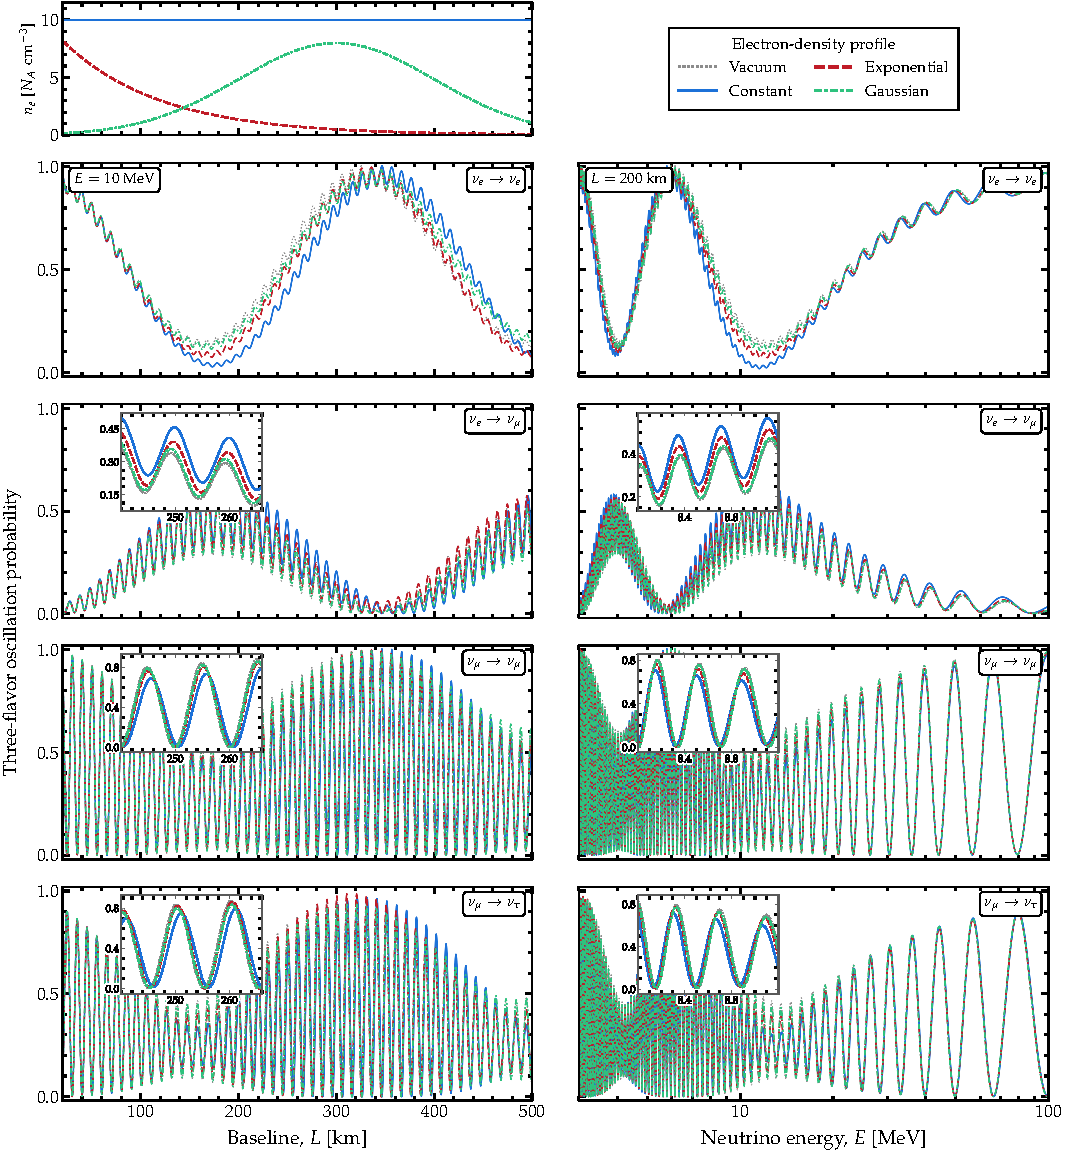
\includegraphics[width=\textwidth]{prob_vs.pdf}
 \caption{\label{fig:prob_vs}Oscillation probabilities of a neutrino that travels through matter, against the distance traveled ({\it left}) and against the neutrino energy ({\it right}). Three matter profiles are drawn, plus the vacuum as a reference. {\it Top left}: the profiles, as the electron number density at each point along the path. The constant profile holds 10~$N_A$ electrons per cm$^3$, with $N_A$ Avogadro's number. The exponential profile starts at that value and halves every 69~km. The Gaussian profile peaks at 8~$N_A$ electrons per cm$^3$, 300~km from the start; its width is 100~km. {\it Rows}: the survival of a $\nu_e$, its conversion into a $\nu_\mu$, the survival of a $\nu_\mu$, and its conversion into a $\nu_\tau$. In the left column the energy is 10~MeV; in the right column the distance is 200~km. Listing~\ref{lst:prob_vs} computes the curves. See notebook \#28 and Sec.~\ref{sec:prob_vs} for details.}
\end{figure*}
%%%%%%%%%%%%%%%%%%%%%%%%%%%%%%%%%%%%%%%%%%%%%%%%%%%%%

Figure~\ref{fig:prob_vs} shows both types of plot, at three flavors, for vacuum and three illustrative choices of the electron density profile: constant density, an exponential fall, and a Gaussian bump near the middle of the path. The constant profile pulls the probabilities furthest from the vacuum ones. The exponential profile follows it near the start of the path, where the density is still high, then drifts back toward the vacuum curves as the density falls. The Gaussian profile does the reverse: it tracks the vacuum curves until the bump, then parts from them.

Listing~\ref{lst:prob_vs} computes the probabilities. \magnus\ takes a constant profile as a single number and a varying profile as a function of the distance traveled. Each column needs four calls: one per matter profile, one in vacuum. Every call receives the full list of distances, or of energies, at once. For the exponential- and constant-density cases, \magnus\ ships functions that take their parameters directly, so the profile need not be supplied separately. Both return the same numbers as the calls in the listing:
\begin{pysnip}
P = oscprob.osc_prob_3nu_matter_exp_density(
 10.0*MEV, 500.0*KM, 0.0, 10.0*NA_CM3,
 100.0*KM, **osc, nu_i=gd.NUE, nu_f=gd.NUE,
 density_is_of_number_of_electrons=True)
# 0.08263484, as in the listing

P = oscprob.\
 osc_prob_3nu_matter_constant_density(
 10.0*MEV, 500.0*KM, 10.0*NA_CM3, **osc,
 nu_i=gd.NUE, nu_f=gd.NUE,
 density_is_of_number_of_electrons=True)
# 0.07132456, as in the listing
\end{pysnip}

%%%%%%%%%%%%%%%%%%%%%%%%%%%%%%%%%%%%%%%%%%%%%%%%%%%%%
\begin{lstlisting}[language=Python, caption={The curves of \figu{prob_vs}: the probability at 5\,000 distances for one energy, then at 3\,000 energies for one distance, for three matter profiles and for vacuum. Each scan is a single call. The constant profile is a number; the two varying ones are functions of the distance traveled. See Sec.~\ref{sec:prob_vs} for details.}, label={lst:prob_vs}, float=tbp]
import numpy as np
import magnus.oscprob as oscprob
import magnus.globaldefs as gd

osc = gd.load_nufit_params('NuFIT 6.1')
KM, MEV = gd.UNIT_KM, gd.UNIT_MEV
# One mole of electrons per cubic centimeter, in the
# natural units that magnus works in
NA_CM3 = gd.N_AV/gd.CONV_CM_TO_INV_EV**3

# Give a constant profile as a single number, and
# a varying one as a function of the distance
# traveled, returning the electron number density
# there.  The distance arrives in eV^-1, like
# every length in magnus
ne_constant = 10.0*NA_CM3

def ne_exponential(l):
    return 10.0*NA_CM3*np.exp(-l/(100.0*KM))

def ne_gaussian(l):
    return 8.0*NA_CM3*np.exp(
     -(l - 300.0*KM)**2/(2*(100.0*KM)**2))

# The first keyword says that the functions return
# an electron number density, not a mass density
KW = dict(density_is_of_number_of_electrons=True,
          rtol=1e-8, atol=1e-10)
PROFILES = (('constant', ne_constant),
            ('exponential', ne_exponential),
            ('gaussian', ne_gaussian))

# Left column: 5,000 distances at one energy.  The
# list of distances goes where a single one would
L = np.linspace(20.0, 500.0, 5000)*KM
P_vs_L = {name: oscprob.osc_prob_matter_std_potential(
 3, ne, 10.0*MEV, L, osc, L0=0.0, **KW)
 for name, ne in PROFILES}

# Right column: 3,000 energies at one distance.
# Asking for the Magnus route sends the scan to the
# engine that carries the energies as a batch
E = np.logspace(np.log10(3.0), 2.0, 3000)*MEV
P_vs_E = {name: oscprob.osc_prob_matter_std_potential(
 3, ne, E, 200.0*KM, osc, L0=0.0,
 strategy='magnus', n_slabs=4000, **KW)
 for name, ne in PROFILES}

# The vacuum curves, for reference
P_vac_L = oscprob.osc_prob_3nu_vacuum(
 10.0*MEV, L, **osc)
P_vac_E = oscprob.osc_prob_3nu_vacuum(
 E, 200.0*KM, **osc)
\end{lstlisting}
%%%%%%%%%%%%%%%%%%%%%%%%%%%%%%%%%%%%%%%%%%%%%%%%%%%%%

The scans over baseline and energy cost very differently. A scan over distance at one energy walks the profile once and reads the probability off at each distance along the way: this is the cumulative engine of Sec.~\ref{sec:engines}. It computes the whole left column of \figu{prob_vs} in under half a second. In contrast, a single walk cannot serve a scan over energy, because the Hamiltonian depends on the energy. The energy-batched scan of Sec.~\ref{sec:engines} covers that case. It applies whenever $\mathbb{H}$ separates in the sense of Sec.~\ref{sec:engines}, as the standard, non-standard-interaction and Lorentz-violating Hamiltonians all do: \magnus\ samples the potential once and carries the energies as a batch dimension. We choose it by passing {\tt strategy='magnus'} to {\tt osc\_prob\_matter\_std\_potential}. It computes the right column of \figu{prob_vs} in about 9~s for each of the varying profiles. {\tt strategy\_info} reports it as {\tt 'separable'}.

By default, {\tt osc\_prob\_matter\_std\_potential} uses {\tt strategy='auto'}, which acts differently on this problem. It sends the energy scan to the hybrid engine of Sec.~\ref{sec:hybrid} instead. That engine transports the state along the instantaneous eigenstates, treating each energy separately. Asking for the Magnus route by name recovers the batched engine; {\tt strategy\_info} reports which one answered:
\begin{pysnip}
info = {}
P = oscprob.osc_prob_matter_std_potential(
 3, ne_exponential, E, 200.0*KM, osc,
 L0=0.0, strategy='magnus',
 strategy_info=info, **KW)
info['engine']   # 'separable'
\end{pysnip}
On a scan of 300 energies through the exponential profile, the energy-batched scan ({\tt strategy='magnus'}) takes 0.8~s against 15.5~s for the hybrid engine ({\tt strategy='auto'}). Both match a reference computed with 16\,000 slabs to better than $10^{-10}$, so nothing is lost by taking the faster one. Asking for the Magnus route is worth doing wherever the Hamiltonian separates this way, as the standard, non-standard-interaction and Lorentz-violating Hamiltonians all do.

%%%%%%%%%%%%%%%%%%%%%%%%%%%%%%%%%%%%%%%%%%%%%%%%%%%%%

\subsection{Layered matter}
\label{sec:arrangement}

%%%%%%%%%%%%%%%%%%%%%%%%%%%%%%%%%%%%%%%%%%%%%%%%%%%%%
\begin{figure}[t!]
 \centering
 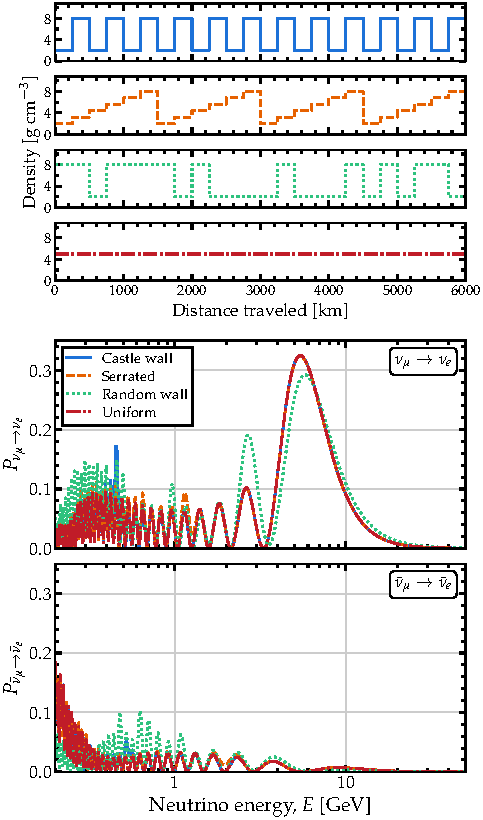
\includegraphics[width=\columnwidth]{density_arrangement.pdf}
 \caption{\label{fig:arrangement}Appearance probability along four piecewise-constant density profiles, for neutrinos ({\it center}) and for antineutrinos ({\it bottom}), computed with \magnus\ at three flavors. The profiles are the top four strips, named in the legend. Each is twenty-four slabs of $250$~km with densities between $2$ and $8$~g~cm$^{-3}$. All four have a mean of $5$~g~cm$^{-3}$ and differ only in the order of the slabs. Slab edges are declared to the refinement, so every curve is the exact product of twenty-four matrix exponentials. See Sec.~\ref{sec:arrangement} for details.}
\end{figure}
%%%%%%%%%%%%%%%%%%%%%%%%%%%%%%%%%%%%%%%%%%%%%%%%%%%%%

Figure~\ref{fig:arrangement} shows the appearance probability along four piecewise-constant profiles, for neutrinos and for antineutrinos. All four have a mean density of $5$~g~cm$^{-3}$ and the same twenty-four slabs; only the order of the slabs changes, but the probabilities change with it. Against the uniform profile, the random wall departs by up to 0.10 in $P_{\nu_\mu \to \nu_e}$ and 0.12 in $P_{\bar{\nu}_\mu \to \bar{\nu}_e}$. 

For neutrinos, the largest feature of the neutrino panel, the broad peak near 6~GeV, is common to all four profiles: it is the matter resonance at 5~g~cm$^{-3}$, which is independent of the arrangement of the slabs. For antineutrinos, there is no counterpart to it, since the matter potential has the opposite sign there.

Only the castle wall has a narrow peak, at 0.46~GeV for neutrinos. The castle-wall densities alternate every 250~km, so the profile repeats every 500~km, which matches the oscillation length in matter at 0.46~GeV. With the two lengths matched, the effect of each alternation adds to the last instead of averaging away. This is the parametric resonance of Sec.~\ref{sec:order_is_the_slab_product}\ \cite{Akhmedov:1988kd, Krastev:1989ix}, on the same profile for which it was solved exactly originally\ \cite{Akhmedov:1998ui}. Antineutrinos have the same peak, but near 0.53~GeV and a third as tall, since the matter potential changes sign and moves the oscillation length with it.

Listing~\ref{lst:arrangement} computes the castle-wall curves. The two calls differ only in {\tt nubar}, which appears here for the first time: it conjugates the mixing matrix and reverses the sign of the matter potential in one step. (Section~\ref{sec:recap} explains why applying one without the other returns a plausible, wrong answer.) The slab edges go to the refinement ladder through {\tt t\_breakpoints}, so no slab straddles a jump. The Hamiltonian is then constant inside every slab, the expansion terminates at its first term, and the answer is the product of twenty-four matrix exponentials. The eight curves take 0.3~s, since the batched engine of Sec.~\ref{sec:engines} reuses the same profile across 400 energies.

%%%%%%%%%%%%%%%%%%%%%%%%%%%%%%%%%%%%%%%%%%%%%%%%%%%%%
\begin{lstlisting}[language=Python, caption={The castle-wall curves of \figu{arrangement}. The profile is a function of position that returns the density of the slab containing that position, and its edges are passed through {\tt t\_breakpoints}, so that no slab of the expansion straddles a jump; within each slab the Hamiltonian is constant, and the result is the exact product of the slab exponentials. The two calls differ only in {\tt nubar}. The other three profiles of the figure differ from this one only in the array {\tt rho}.}, label={lst:arrangement}, float=tbp]
import numpy as np
import magnus.oscprob as oscprob
import magnus.globaldefs as gd

osc = gd.load_nufit_params('NuFIT 6.1')
# 24 slabs of 250 km, alternating 2 and 8 g/cm^3
n, width = 24, 250.0*gd.UNIT_KM
rho = np.where(np.arange(n) % 2 == 0, 2.0, 8.0)
edges = np.arange(n + 1)*width

def castle_wall(l):
    """The density at position l, in g/cm^3."""
    k = np.searchsorted(edges, l, side='right') - 1
    return rho[np.clip(k, 0, n - 1)]

E = np.logspace(-0.7, 1.7, 400)*gd.UNIT_GEV
# The slab edges are declared, so no slab straddles a
# jump; within each, one term of the expansion is exact
P, Pbar = [oscprob.osc_prob_matter_std_potential(
    3, castle_wall, E, n*width, osc,
    t_breakpoints=edges[1:-1], nubar=nubar,
    nu_i=gd.NUMU, nu_f=gd.NUE,
    density_matter_is_in_g_per_cm3=True,
    rtol=1.0e-8, atol=1.0e-10)
    for nubar in (False, True)]
\end{lstlisting}
%%%%%%%%%%%%%%%%%%%%%%%%%%%%%%%%%%%%%%%%%%%%%%%%%%%%%

%%%%%%%%%%%%%%%%%%%%%%%%%%%%%%%%%%%%%%%%%%%%%%%%%%%%%

\subsection{Bi-probability plot}
\label{sec:biprobability}

%%%%%%%%%%%%%%%%%%%%%%%%%%%%%%%%%%%%%%%%%%%%%%%%%%%%%
\begin{figure}[t!]
 \centering
 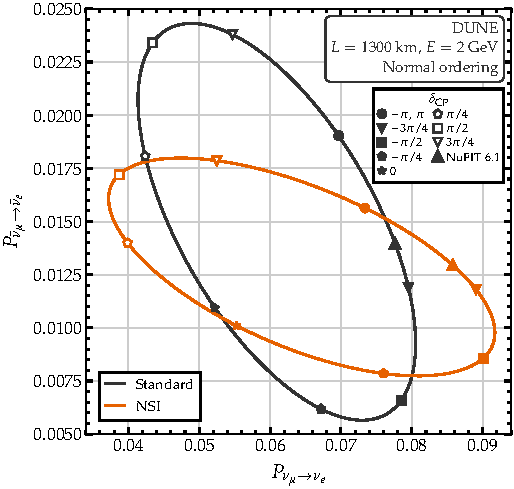
\includegraphics[width=\columnwidth]{biprobability.pdf}
 \caption{\label{fig:biprobability}Bi-probability plot: appearance probability of an antineutrino vs.~a neutrino, computed with \magnus\ through matter of constant density $3$~g~cm$^{-3}$, on a baseline equal to that of DUNE, comparing standard oscillations and non-standard interactions (NSI). The NSI couplings are those of \figu{bsm}: $\varepsilon_{ee} = 0.10$, $\varepsilon_{e\mu} = 0.05$, and $\varepsilon_{\mu\tau} = 0.03$. Listing~\ref{lst:biprobability} shows the code snippet to make this figure. See notebooks \#05 and \#28, and Sec.~\ref{sec:biprobability} for details.}
\end{figure}
%%%%%%%%%%%%%%%%%%%%%%%%%%%%%%%%%%%%%%%%%%%%%%%%%%%%%

Figure~\ref{fig:biprobability} shows a bi-probability plot\ \cite{Minakata:2001qm}: the antineutrino appearance probability against the neutrino one. Listing~\ref{lst:biprobability} shows the code to generate it. Each value of $\delta_{\rm CP}$ is one point, so taking the phase through its range traces a closed curve. The two curves are the standard case and the same case with non-standard interactions. They cross. A measurement landing on a crossing reads as the standard case at one value of $\delta_{\rm CP}$ and as the non-standard one at another, so a new interaction can pass for a shift in the phase. Separating the two takes a second measurement, at another energy or baseline.

The two curves of \figu{biprobability} come from the same call with a different Hamiltonian, which is what makes a degeneracy easy to draw: any two hypotheses that a measurement might confuse---NSI vs.~a shifted CP phase, or the mass ordering against vs.~the $\theta_{23}$ octant---go on one plot by swapping the matrix. Notebook \#17 does that for the ordering and the octant.

\begin{lstlisting}[language=Python, caption={The two bi-probability curves of \figu{biprobability}. {\tt locus} takes a wrapper through $\delta_{\rm CP}$, evaluating a neutrino and an antineutrino at each of its values. The baseline is that of DUNE and the constant density, that of the Earth's crust. No tolerance appears in the calculation because a constant Hamiltonian ends the Magnus expansion at its first term exactly. The curves are drawn twice: first by {\tt plotting.plot\_biprobability}, which takes styling choices, then by {\tt matplotlib} directly. See notebooks \#05 and \#28, and Sec.~\ref{sec:biprobability} for details.}, label={lst:biprobability}, float=tbp]
import numpy as np
import matplotlib.pyplot as plt
import magnus.oscprob as oscprob
import magnus.globaldefs as gd
import magnus.plotting as plotting

E, L, rho = 2.0*gd.UNIT_GEV, 1300.0*gd.UNIT_KM, 3.0
kw = dict(nu_i=gd.NUMU, nu_f=gd.NUE,
          density_matter_is_in_g_per_cm3=True)
eps = dict(eps_ee=0.10, eps_em=0.05, eps_mt=0.03)
std = oscprob.osc_prob_3nu_matter_constant_density
nsi = oscprob.osc_prob_3nu_matter_nsi_constant_density

def locus(wrapper, **couplings):
    """(P_mu e, P_mubar ebar) once around delta_CP."""
    out = []
    for dcp in np.linspace(-np.pi, np.pi, 181):
        P = [wrapper(E, L, rho, nubar=nubar, dCP=dcp,
                     **couplings, **kw)
             for nubar in (False, True)]
        out.append(P)
    return np.array(out)

P_std = locus(std)
P_nsi = locus(nsi, **eps)

# With the shipped plotter
fig, ax = plotting.plot_biprobability(
    [P_std[:, 0], P_nsi[:, 0]],
    [P_std[:, 1], P_nsi[:, 1]],
    labels=['Standard', 'NSI'])

# With matplotlib directly
fig, ax = plt.subplots()
for P, label in ((P_std, 'Standard'), (P_nsi, 'NSI')):
    ax.plot(P[:, 0], P[:, 1], label=label)
ax.set_xlabel(r'$P_{\nu_\mu \to \nu_e}$')
ax.set_ylabel(r'$P_{\bar\nu_\mu \to \bar\nu_e}$')
ax.legend()
\end{lstlisting}

%%%%%%%%%%%%%%%%%%%%%%%%%%%%%%%%%%%%%%%%%%%%%%%%%%%%%

\subsection{The Earth}
\label{sec:prem}

%%%%%%%%%%%%%%%%%%%%%%%%%%%%%%%%%%%%%%%%%%%%%%%%%%%%%
\begin{figure}[t!]
 \centering
 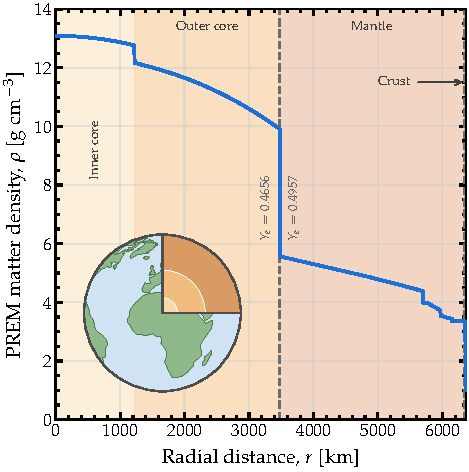
\includegraphics[width=\columnwidth]{prem_profile.pdf}
 \caption{\label{fig:prem}The PREM density profile\ \cite{Dziewonski:1981xy} against radial distance, with a cut-away globe showing the same layers in the same colors. The electron fraction changes at three radii, marked by the dashed lines: from $0.4656$ to $0.4957$ at the core-mantle boundary, then to $0.4952$ at $6\,346.6$~km and to $0.5551$ in the ocean at $6\,368$~km, the last two too close together to separate here. \magnus\ places a slab edge wherever a chord crosses one of the nine PREM layer boundaries, so that no slab straddles a density jump. See Sec.~\ref{sec:prem} for details.}
\end{figure}
%%%%%%%%%%%%%%%%%%%%%%%%%%%%%%%%%%%%%%%%%%%%%%%%%%%%%

Figure~\ref{fig:prem} shows the density profile \magnus\ uses for the Earth, the Preliminary Reference Earth Model (PREM)\ \cite{Dziewonski:1981xy}, built from seismic data. The Earth is treated as a layered, spherically symmetric with a radius of $R_\oplus = 6\,371$~km. The density falls from 13.1~g~cm$^{-3}$ at the core to 1~g~cm$^{-3}$ (the density of water) at the surface, smoothly inside each of nine shells and in jumps between them. The largest jump is at the core-mantle boundary, $3480$~km from the center, where the density drops from $9.90$ to $5.57$~g~cm$^{-3}$. The electron fraction, $Y_e$, reflects the chemical composition of the Earth and so changes with radial distance, but not at every PREM jump. \magnus\ resolves it thus: 0.4656 in the core, 0.4957 in the mantle, 0.4952 in the crust, and 0.5551 in the ocean. They are {\tt electron\_fraction\_core}, {\tt electron\_fraction\_mantle}, {\tt electron\_fraction\_crust}, and {\tt electron\_fraction\_ ocean} in the {\tt earth} module.

The trajectory of a neutrino through the Earth is determined by its zenith angle at the detector, $\theta_z$. The detector sits on the surface by default. (Section~\ref{sec:underground} shows how to place sources and detectors underground.) A core-crossing neutrino arriving from straight below has $\cos\theta_z = -1$ and crosses an Earth diameter. One arriving along the horizon has $\cos\theta_z = 0$ and does travel inside the Earth at all (for a detector on the surface). Between them, the chord reaches a minimum radius of $R_\oplus \sqrt{1 - \cos^2\theta_z}$, so a shallower trajectory, closer to horizontal, samples only the outer PREM shells. 

For a given zenith angle, the baseline is returned via, \eg,
\begin{pysnip}
import magnus.earth as earth

costhz = -0.9
L = earth.distance_traveled_inside_earth(
    costhz)                    # 11467.8 km
\end{pysnip}
A chord meets every PREM boundary it reaches twice, once going in and once coming out. For instance, at $\cos\theta_z = -0.9$, the closest approach to the Earth's center is $2\,777$~km, which leaves eight of the nine boundaries above it and sixteen crossings along the path:
\begin{pysnip}
edges = earth.prem_layer_edges_along_chord(
    costhz)
len(edges)                     # 16
\end{pysnip}
For a given {\tt costhz}, every {\tt osc\_prob\_*\_earth} wrapper computes those positions itself and passes them to the refinement as {\tt t\_breakpoints}. A slab edge is automatically placed on every crossing, at every level of the refinement ladder and at whatever tolerance the method is requested. 

The wrappers define the neutrino trajectory via the zenith angle and the baseline. A given {\tt costhz} determines---internally in the wrapper---the density at each point of the chord, the electron fraction there, and the slab edges. The baseline needs converting, since {\tt earth} reports kilometers. At three flavors, for a 10-GeV neutrino, $P_{\nu_\mu \to \nu_e}$ is computed via
\begin{pysnip}
import magnus.oscprob as oscprob
import magnus.globaldefs as gd

P = oscprob.osc_prob_3nu_earth(
    10.0*gd.UNIT_GEV, costhz=costhz,
    L=L*gd.UNIT_KM)
P[gd.NUMU][gd.NUE]             # 0.127041
\end{pysnip}
By default, the electron fraction changes through the PREM, as explained above. Passing {\tt electron\_fraction} to the wrappers overrides this by replacing those values with a single one for the whole Earth. At $5$~GeV along this chord, the two probability calculations differ by $0.08$ in $P_{\nu_\mu \to \nu_e}$:
\begin{pysnip}
kw = dict(costhz=costhz, L=L*gd.UNIT_KM,
          nu_i=gd.NUMU, nu_f=gd.NUE)
E = 5.0*gd.UNIT_GEV

oscprob.osc_prob_3nu_earth(E, **kw) # 0.1009
                               
oscprob.osc_prob_3nu_earth(
    E, **kw, electron_fraction=0.5) # 0.0207
                               
\end{pysnip}

%%%%%%%%%%%%%%%%%%%%%%%%%%%%%%%%%%%%%%%%%%%%%%%%%%%%%

\subsubsection{Neutrinos \& antineutrinos, 2--5 flavors}
\label{sec:nu_nubar}

%%%%%%%%%%%%%%%%%%%%%%%%%%%%%%%%%%%%%%%%%%%%%%%%%%%%%
\begin{figure}[t!]
 \centering
 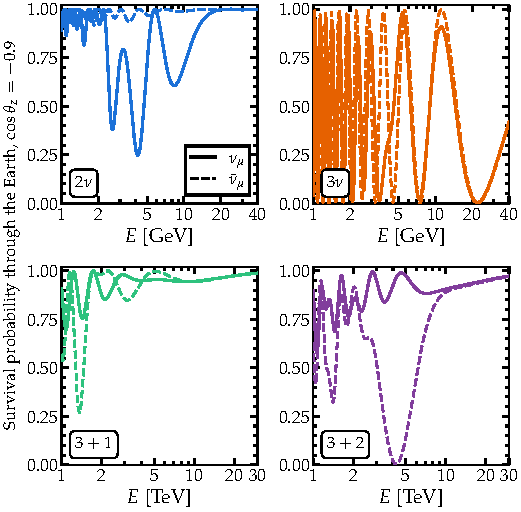
\includegraphics[width=\columnwidth]{nu_nubar_earth.pdf}
 \caption{\label{fig:nu_nubar}Survival probability of $\nu_\mu$ and $\bar{\nu}_\mu$ along a PREM chord at $\cos\theta_z = -0.9$, computed with \magnus. {\it Top}: two flavors, the $(\nu_e, \nu_\mu)$ reduction of the 1--3 sector, and three flavors, both from $1$ to $40$~GeV. {\it Bottom}: $3+1$ and $3+2$ from $1$ to $30$~TeV, where an eV-scale splitting places its resonance, with $\sin^2\theta_{14} = \sin^2\theta_{24} = 0.10$ and $\Delta m^2_{41} = 1$~eV$^2$, joined in the $3+2$ panel by $\sin^2\theta_{15} = \sin^2\theta_{25} = 0.06$ and $\Delta m^2_{51} = 1.7$~eV$^2$. Listing~\ref{lst:nu_nubar} draws all four pairs. See notebooks \#15 and \#28, and Sec.~\ref{sec:nu_nubar} for details.}
\end{figure}
%%%%%%%%%%%%%%%%%%%%%%%%%%%%%%%%%%%%%%%%%%%%%%%%%%%%%

Figure~\ref{fig:nu_nubar} shows $\nu_\mu$ and $\bar{\nu}_\mu$ survival probabilities along the same core-crossing $\cos \theta_z = -0.9$ chord as before, at two to five flavors. Listing~\ref{lst:nu_nubar} draws all eight curves. One dictionary carries the chord, the channel, and the tolerances through every call, so the four flavor counts differ only in the wrapper's name, the energy range, and the mixing 3+1 and 3+2 one add.

In the top row, the ordinary matter resonance depletes the $\nu_\mu$ and leaves the $\bar{\nu}_\mu$ unaffected, because the matter potential enters their Hamiltonians with opposite signs. The two-flavor panel shows this cleanly. A $(\nu_e, \nu_\mu)$ system carries no $\theta_{23}$ oscillation, so the only structure left is resonant: the $\nu_\mu$ dips deeply at a few GeV, while the $\bar{\nu}_\mu$ stays near one across the panel. The three-flavor panel restores the $\theta_{23}$ oscillation, which is near-maximal. Both curves then sweep between zero and one several times over, so the resonance stops being easily identifiable. The resonance survives as a phase offset between the $\nu_\mu$ and the $\bar{\nu}_\mu$ below about $10$~GeV. That offset closes as the energy rises, until the two curves coincide above $20$~GeV.

In the bottom row, for 3+1 and 3+2, the roles are reversed. A sterile state feels no matter potential at all. A sterile state feels no matter potential at all. The active states all feel the same neutral-current potential, $V_{\rm NC}$, which cancels out of the oscillation. The $\nu_e$ keeps the charged-current potential, $V_{\rm CC}$, since it alone scatters off electrons that way. Each sterile state carries $-V_{\rm NC}$. A resonance needs the potential to act on the lighter of the two mass states that mix. For two and three flavors, it acts on the $\nu_e$, which for normal mass ordering is mostly the lighter of that pair, so the $\nu_\mu$ is the one that resonates and gets depleted. For 3+1 and 3+2, the potential acts on the sterile state, which a positive $\Delta m^2_{41}$ makes the heavier, so the $\bar{\nu}_\mu$ is depleted instead. Section~\ref{sec:bsm} locates the resonance in energy. 

The resonance is legible here in the way $\bar{\nu}_\mu$ falls into an isolated dip near $1.4$~TeV, while the $\nu_\mu$ stays high across the panel. Searches for a sterile state in atmospheric neutrinos look for exactly this dip~\cite{IceCube:2016rnb, IceCube:2020phf}. A second sterile state adds a second dip at three times the energy, deeper than the first and much wider. Above $10$~TeV, both curves come back together near one.

%%%%%%%%%%%%%%%%%%%%%%%%%%%%%%%%%%%%%%%%%%%%%%%%%%%%%
\begin{lstlisting}[language=Python, caption={The $\nu_\mu$ and $\bar{\nu}_\mu$ probability curves of \figu{nu_nubar}. Only {\tt nubar} separates the two members of a pair at the same flavor count. See notebooks \#15 and \#28, and Sec.~\ref{sec:nu_nubar} for details.}, label={lst:nu_nubar}, float=tbp]
import numpy as np
import magnus.oscprob as oscprob
import magnus.earth as earth
import magnus.globaldefs as gd

costhz = -0.9
L = earth.distance_traveled_inside_earth(costhz) \
 *gd.UNIT_KM
kw = dict(costhz=costhz, L=L, nu_i=gd.NUMU,
          nu_f=gd.NUMU, rtol=1.0e-8, atol=1.0e-10)

def both_signs(wrapper, E, **params):
    """Survival probability, for a nu then a nubar."""
    return [wrapper(E, nubar=nubar, **params, **kw)
            for nubar in (False, True)]

# Two flavors is the (nu_e, nu_mu) reduction of the 1-3
# sector, so it takes that one angle and splitting by
# name.  Every wrapper above two flavors defaults to
# the same NuFIT 6.1 set, so it needs none passed.
osc = gd.load_nufit_params('NuFIT 6.1')
E = np.logspace(0, np.log10(40), 260)*gd.UNIT_GEV
P2, P2bar = both_signs(oscprob.osc_prob_2nu_earth, E,
                       sth=osc['s13'], Dm2=osc['D31'])
P3, P3bar = both_signs(oscprob.osc_prob_3nu_earth, E)

# The sterile pairs run three decades higher, where an
# eV-scale splitting places its resonance
E_TEV = np.logspace(0, np.log10(30), 200)*gd.UNIT_TEV
s4 = dict(s14=np.sqrt(0.10), s24=np.sqrt(0.10), s34=0.0,
          D41=1.0)
s5 = dict(**s4, s15=np.sqrt(0.06), s25=np.sqrt(0.06),
          s35=0.0, D51=1.7)
P4, P4bar = both_signs(oscprob.osc_prob_4nu_earth,
                       E_TEV, **s4)
P5, P5bar = both_signs(oscprob.osc_prob_5nu_earth,
                       E_TEV, **s5)
\end{lstlisting}
%%%%%%%%%%%%%%%%%%%%%%%%%%%%%%%%%%%%%%%%%%%%%%%%%%%%%

%%%%%%%%%%%%%%%%%%%%%%%%%%%%%%%%%%%%%%%%%%%%%%%%%%%%%

\subsubsection{Probabilities between two locations}
\label{sec:named_baselines}

%%%%%%%%%%%%%%%%%%%%%%%%%%%%%%%%%%%%%%%%%%%%%%%%%%%%%
\begin{figure*}[t!]
 \centering
 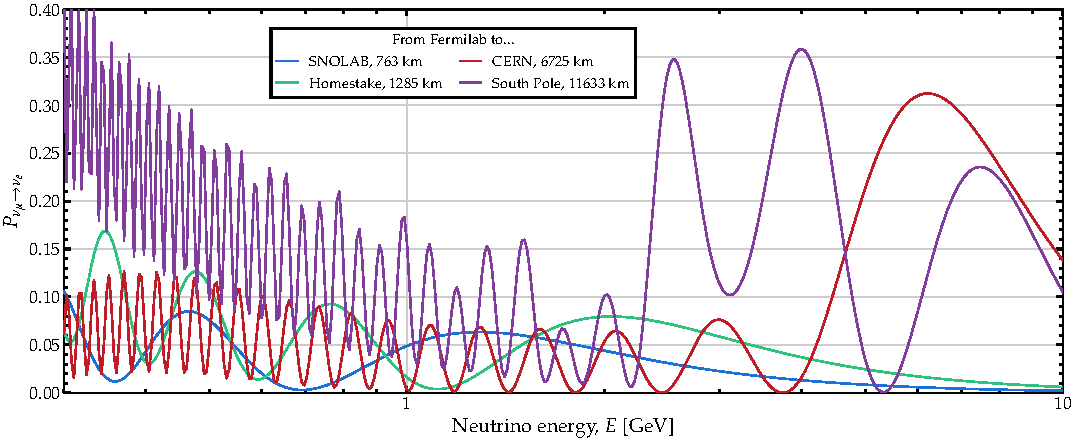
\includegraphics[width=\textwidth]{named_baselines.pdf}
 \caption{\label{fig:named_baselines}Appearance probability $P_{\nu_\mu \to \nu_e}$ against energy for a beam sent from Fermilab to four named sites, computed with \magnus\ along the PREM chord joining each pair of locations, at the layered composition of Section~\ref{sec:prem}. The legend gives the chord length of each. The two shortest show the pattern of a beam experiment, a first oscillation maximum at a few GeV with faster oscillations below it. The two longest cross the matter resonance, which is why the probability along them is several times larger. Listing~\ref{lst:named} draws the curves. See notebooks \#04 and \#28, and Sec.~\ref{sec:named_baselines} for details.}
\end{figure*}
%%%%%%%%%%%%%%%%%%%%%%%%%%%%%%%%%%%%%%%%%%%%%%%%%%%%%

%%%%%%%%%%%%%%%%%%%%%%%%%%%%%%%%%%%%%%%%%%%%%%%%%%%%%
\begin{table}[t!]
{\normalsize
\begin{tabular}{@{}p{2.6cm}p{2.5cm}p{2.7cm}@{}}
 Site name & Latitude & Longitude \\
 \hline
 {\tt baikal} & $51^\circ\,45'\,54''$ & $104^\circ\,24'\,54''$ \\
 {\tt cern} & $46^\circ\,14'\,1.8''$ & $6^\circ\,3'\,11.4''$ \\
 {\tt desy} & $53^\circ\,34'\,19.79''$ & $9^\circ\,52'\,27.59''$ \\
 {\tt ess} & $55^\circ\,44'\,6''$ & $13^\circ\,15'\,5.04''$ \\
 {\tt fermilab} & $41^\circ\,49'\,55''$ & $-88^\circ\,15'\,26''$ \\
 {\tt gran\_sasso} & $42^\circ\,25'\,15.8''$ & $13^\circ\,30'\,58.43''$ \\
 {\tt homestake} & $44^\circ\,21'\,5.76''$ & $-103^\circ\,45'\,4.68''$ \\
 {\tt kamioka} & $36^\circ\,25'\,50.05''$ & $137^\circ\,18'\,41.15''$ \\
 {\tt km3net\_arca} & $36^\circ\,16'\,0''$ & $16^\circ\,6'\,0''$ \\
 {\tt km3net\_orca} & $42^\circ\,48'\,0''$ & $6^\circ\,2'\,0''$ \\
 {\tt north\_pole} & $90^\circ\,0'\,0''$ & $0^\circ\,0'\,0''$ \\
 {\tt pyhaasalmi} & $63^\circ\,39'\,31''$ & $26^\circ\,2'\,28''$ \\
 {\tt snolab} & $46^\circ\,28'\,18''$ & $-81^\circ\,11'\,12''$ \\
 {\tt south\_pole} & $-90^\circ\,0'\,0''$ & $0^\circ\,0'\,0''$ \\
 {\tt tokai} & $36^\circ\,27'\,59''$ & $140^\circ\,36'\,24''$ \\
\end{tabular}
}
\caption{\label{tab:sites}The fifteen locations {\tt magnus.earth} carries by name, with the coordinates it stores for each. A name passed as {\tt loc\_ini} or {\tt loc\_fin} stands for the pair beside it. Coordinates are in degrees, minutes and seconds, which is the form the module stores and the one {\tt loc\_ini} and {\tt loc\_fin} accept; {\tt earth.dms\_to\_decimal} returns the same coordinate in decimal degrees.}
\end{table}
%%%%%%%%%%%%%%%%%%%%%%%%%%%%%%%%%%%%%%%%%%%%%%%%%%%%%

\textit{Locations given as coordinates.---}Earlier examples specified a trajectory through the Earth by its arrival direction, given by its zenith angle. A long-baseline experiment is described by where the beam is made and where it is detected. The Earth wrappers accept that form, too. Passing {\tt loc\_ini} and {\tt loc\_fin} replaces both {\tt costhz} and {\tt L}: the chord joining the two sites becomes the baseline; its direction fixes which PREM shells that chord crosses. Each location is a (latitude, longitude) pair, with both stated in degrees, minutes and seconds. North and east are positive; south and west are negative. The sign is read from the first non-zero part:
\begin{pysnip}
# (degree, minute, second), north and east
# positive, south and west negative
fnal = ((41, 49, 55), (-88, 15, 26))
hs = ((44, 21, 5.76), (-103, 45, 4.68))
P = oscprob.osc_prob_3nu_earth(
    2.0*gd.UNIT_GEV, loc_ini=fnal,
    loc_fin=hs, nu_i=gd.NUMU, nu_f=gd.NUE)
P                              # 0.0794317
\end{pysnip}

A chord between two surface locations is a density palindrome. The trajectory meets every radius twice, so \magnus\ evaluates the Hamiltonian over the first half and mirrors the rest; Sec.~\ref{sec:cost} gives what that saves. Naming two locations also fixes the baseline at the whole chord length between them. An {\tt L} passed alongside is discarded.

\smallskip

\textit{Named sites.---}Figure~\ref{fig:named_baselines} shows the appearance probability $P_{\nu_\mu \to \nu_e}$ along four chords, each running from Fermilab to a named site. Listing~\ref{lst:named} shows how to compute them. Table~\ref{tab:sites} lists the fifteen locations the {\tt earth} module carries by name. Passing a name is the same as passing the coordinates beside it:
\begin{pysnip}
P = oscprob.osc_prob_3nu_earth(
    2.0*gd.UNIT_GEV, 
    loc_ini='fermilab', loc_fin='homestake',
    nu_i=gd.NUMU, nu_f=gd.NUE)
P                              # 0.0794317
\end{pysnip}
The two calls return the same probability. The named form is the one Listing~\ref{lst:named} makes. How deep a chord runs varies. The one to SNOLAB stays inside the crust, $11$~km down at its deepest. The one to Homestake, which is the DUNE baseline, reaches $33$~km. The one to CERN reaches $960$~km, into the lower mantle. The one to the South Pole reaches $3\,770$~km, through the outer core. 

%%%%%%%%%%%%%%%%%%%%%%%%%%%%%%%%%%%%%%%%%%%%%%%%%%%%%
\begin{lstlisting}[language=Python, caption={The four curves of \figu{named_baselines}. Two site names replace {\tt costhz} and {\tt L}: the wrapper takes the chord between them as the baseline and its direction as the trajectory. {\tt chord\_length\_inside\_earth} returns the chord length. Site names are in \tabl{sites}. See notebooks \#04 and \#28, and Sec.~\ref{sec:named_baselines} for details.}, label={lst:named}, float=tbp]
import numpy as np
import magnus.oscprob as oscprob
import magnus.earth as earth
import magnus.globaldefs as gd

E = np.logspace(np.log10(0.3), 1.0, 400)*gd.UNIT_GEV
sites = ('snolab', 'homestake', 'cern', 'south_pole')

# Two site names replace costhz and L: the chord
# between them is the baseline
P = {site: oscprob.osc_prob_3nu_earth(
         E, loc_ini='fermilab', loc_fin=site,
         nu_i=gd.NUMU, nu_f=gd.NUE,
         rtol=1.0e-8, atol=1.0e-10)
     for site in sites}

# The chord itself, in km, for a legend
a = earth.loc_coords_dms['fermilab']
b = earth.loc_coords_dms['homestake']
L_km = earth.chord_length_inside_earth(
    a['lat'], a['lon'], b['lat'], b['lon'])
print('%.0f km' % L_km)   # 1285
\end{lstlisting}
%%%%%%%%%%%%%%%%%%%%%%%%%%%%%%%%%%%%%%%%%%%%%%%%%%%%%

%%%%%%%%%%%%%%%%%%%%%%%%%%%%%%%%%%%%%%%%%%%%%%%%%%%%%

\subsubsection{New physics}
\label{sec:bsm}

%%%%%%%%%%%%%%%%%%%%%%%%%%%%%%%%%%%%%%%%%%%%%%%%%%%%%
\begin{figure}[t!]
 \centering
 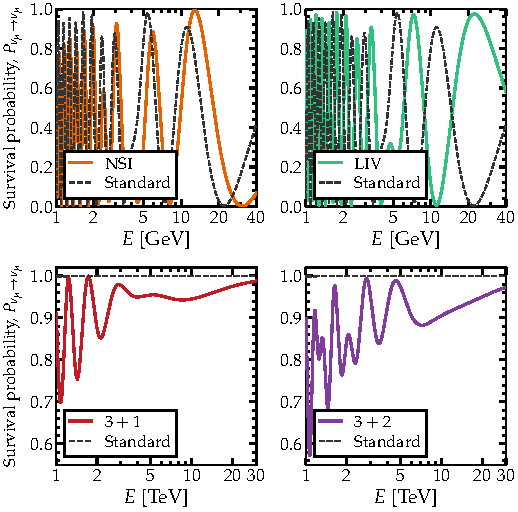
\includegraphics[width=\columnwidth]{bsm.pdf}
 \caption{\label{fig:bsm}Muon-neutrino survival probability $P_{\nu_\mu \to \nu_\mu}$ along a PREM chord at $\cos\theta_z = -0.9$, computed with \magnus\ for four departures from the standard three-flavor case. {\it Top left}: non-standard interactions with $\varepsilon_{ee} = 0.10$, $\varepsilon_{e\mu} = 0.05$ and $\varepsilon_{\mu\tau} = 0.03$. {\it Top right}: isotropic CPT-even Lorentz-violating term with eigenvalues $b_1 = b_2 = 0$ and $b_3 = 5.4 \cdot 10^{-14}$~eV, the value that advances the phase by $\pi$ over this chord. {\it Bottom}: the 3+1 and 3+2 systems of \figu{nu_nubar}, where the eV-scale splittings, $\Delta m_{41}^2$ and $\Delta m_{51}^2$, respectively, place the matter resonance at the TeV scale. Listing~\ref{lst:bsm} draws the curves. See notebook \#07, \#08, \#09, and \#28, and Sec.~\ref{sec:bsm} for details.}
\end{figure}
%%%%%%%%%%%%%%%%%%%%%%%%%%%%%%%%%%%%%%%%%%%%%%%%%%%%%

%%%%%%%%%%%%%%%%%%%%%%%%%%%%%%%%%%%%%%%%%%%%%%%%%%%%%
\begin{lstlisting}[language=Python, caption={The five scenarios of \figu{bsm}, in six calls: the standard case is computed twice, once for each energy range. Every call shares the chord, the channel and the tolerances, differing only in the wrapper's name and in the parameters the extra term brings. See notebook \#07, \#08, \#09, and \#28, and Sec.~\ref{sec:bsm} for details.}, label={lst:bsm}, float=tbp]
import numpy as np
import magnus.oscprob as oscprob
import magnus.earth as earth
import magnus.globaldefs as gd

costhz = -0.9
L = earth.distance_traveled_inside_earth(costhz) \
 *gd.UNIT_KM
kw = dict(costhz=costhz, L=L, nu_i=gd.NUMU,
          nu_f=gd.NUMU, rtol=1.0e-8, atol=1.0e-10)
E = np.logspace(0, np.log10(40), 260)*gd.UNIT_GEV
# Three decades up is where an eV-scale splitting
# places its matter resonance
E_TEV = np.logspace(0, np.log10(30), 200)*gd.UNIT_TEV

eps = dict(eps_ee=0.10, eps_em=0.05, eps_mt=0.03)
liv = dict(b1=0.0, b2=0.0, b3=np.pi/L, Lambda=1.0,
           sxi12=0.0, sxi23=1.0/np.sqrt(2.0),
           sxi13=0.0, dxiCP=0.0, n_liv=0)
s4 = dict(s14=np.sqrt(0.10), s24=np.sqrt(0.10),
          s34=0.0, D41=1.0)
s5 = dict(**s4, s15=np.sqrt(0.06),
          s25=np.sqrt(0.06), s35=0.0, D51=1.7)

# The same call each time, a different extra term
P_std = oscprob.osc_prob_3nu_earth(E, **kw)
P_nsi = oscprob.osc_prob_3nu_earth_nsi(E, **eps, **kw)
P_liv = oscprob.osc_prob_3nu_earth_liv(E, **liv, **kw)
P_std_tev = oscprob.osc_prob_3nu_earth(E_TEV, **kw)
P_3p1 = oscprob.osc_prob_4nu_earth(E_TEV, **s4, **kw)
P_3p2 = oscprob.osc_prob_5nu_earth(E_TEV, **s5, **kw)
\end{lstlisting}
%%%%%%%%%%%%%%%%%%%%%%%%%%%%%%%%%%%%%%%%%%%%%%%%%%%%%

Figure~\ref{fig:bsm} shows four departures from the standard three-flavor case along one deep Earth chord: non-standard interactions\ \cite{Farzan:2017xzy}, Lorentz-invariance violation\ \cite{Kostelecky:2003xn, Kostelecky:2011gq}, one sterile state\ \cite{Gariazzo:2015rra, Dentler:2018sju}, and two sterile states\ \cite{Sorel:2003hf}. Each adds a different term to the Hamiltonian. Listing~\ref{lst:bsm} shows how all calls to \magnus\ are similar, only the wrapper name changing and being given extra new-physics parameters.

Figure~\ref{fig:sterile_scan} scans the sterile parameters themselves. Nothing about the call changes across the plane: the wrapper takes $\Delta m^2_{41}$ and $\theta_{14}$ like any other argument, so a map is a comprehension over the two of them, and Listing~\ref{lst:sterile_scan} is the whole of it. What the map shows is the reversal of Sec.~\ref{sec:nu_nubar} laid out in parameter space. The $\nu_\mu$ panels barely move, reaching $-0.27$ at their darkest. The $\bar{\nu}_\mu$ panels carry a resonance band at $\Delta m^2_{41} \simeq 1$~eV$^2$ that removes up to $0.87$ of the flux. The band closes at both ends of the mixing range, since the effect vanishes at $\theta_{14} = 0$ and again at maximal mixing.

%%%%%%%%%%%%%%%%%%%%%%%%%%%%%%%%%%%%%%%%%%%%%%%%%%%%%
\begin{figure}[t!]
 \centering
 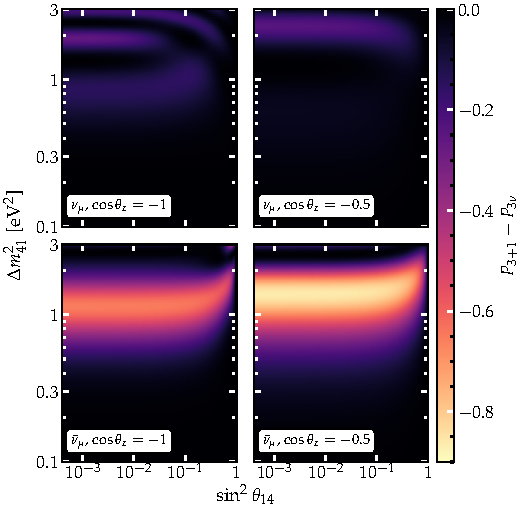
\includegraphics[width=\columnwidth]{sterile_scan.pdf}
 \caption{\label{fig:sterile_scan}Change in the muon-neutrino survival probability when one sterile state is added, $P_{3+1} - P_{3\nu}$, as a function of $\Delta m_{41}^2$ and $\sin^2 \theta_{14}$, at a fixed energy of $5$~TeV. {\it Top row}: $\nu_\mu$. {\it Bottom row}: $\bar{\nu}_\mu$. {\it Left column}: a core-crossing chord, $\cos\theta_z = -1$. {\it Right column}: a shallower one, $\cos\theta_z = -0.5$. The other sterile parameters are held at $\sin^2\theta_{24} = 0.10$ and $\theta_{34} = 0$. Each panel is $80 \times 80$ probabilities. See notebooks \#7 and \#28, and Sec.~\ref{sec:bsm} for details.}
\end{figure}
%%%%%%%%%%%%%%%%%%%%%%%%%%%%%%%%%%%%%%%%%%%%%%%%%%%%%

%%%%%%%%%%%%%%%%%%%%%%%%%%%%%%%%%%%%%%%%%%%%%%%%%%%%%
\begin{lstlisting}[language=Python, caption={The four panels of \figu{sterile_scan}. The standard, three-flavor probability case is computed once per panel. The other three panels change {\tt costhz} and {\tt nubar}. See notebooks \#07 and \#28, and Sec.~\ref{sec:bsm} for details.}, label={lst:sterile_scan}, float=tbp]
import numpy as np
import magnus.oscprob as oscprob
import magnus.earth as earth
import magnus.globaldefs as gd

E = 5.0*gd.UNIT_TEV
D41 = np.logspace(np.log10(0.1), np.log10(3.0), 80)
S14 = np.logspace(np.log10(0.02), 0.0, 80)
s24 = np.sqrt(0.10)

def panel(costhz, nubar):
    """One chord and one sign, over the whole plane."""
    L = earth.distance_traveled_inside_earth(costhz) \
     *gd.UNIT_KM
    kw = dict(costhz=costhz, L=L, nu_i=gd.NUMU,
              nu_f=gd.NUMU, nubar=nubar,
              rtol=1.0e-8, atol=1.0e-10)
    # Standard 3nu oscillations
    std = oscprob.osc_prob_3nu_earth(E, **kw)
    return np.array([[oscprob.osc_prob_4nu_earth(
        E, s14=s, s24=s24, s34=0.0, D41=d, **kw)
        - std for s in S14] for d in D41])

# Change between 3nu and 3+1 survival probability
dP = {(cz, nb): panel(cz, nb)
      for cz in (-1.0, -0.5) for nb in (False, True)}
\end{lstlisting}
%%%%%%%%%%%%%%%%%%%%%%%%%%%%%%%%%%%%%%%%%%%%%%%%%%%%%

%%%%%%%%%%%%%%%%%%%%%%%%%%%%%%%%%%%%%%%%%%%%%%%%%%%%%

\subsubsection{Earth oscillograms}
\label{sec:earth_oscillograms}

%%%%%%%%%%%%%%%%%%%%%%%%%%%%%%%%%%%%%%%%%%%%%%%%%%%%%
\begin{figure}[t!]
 \centering
 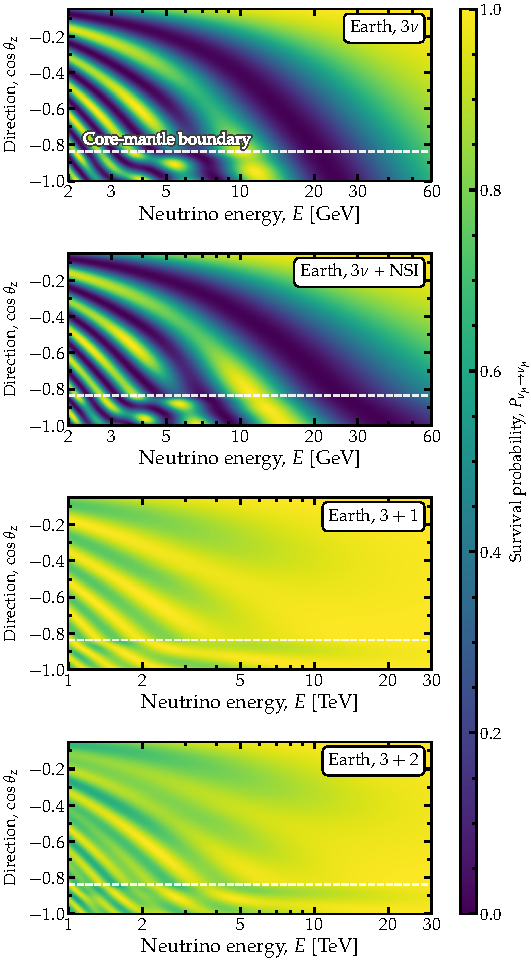
\includegraphics[width=\columnwidth]{earth_oscillogram.pdf}
 \caption{\label{fig:oscillogram}Oscillogram: the $\nu_\mu$ survival probability, $P_{\nu_\mu \to \nu_\mu}$, over neutrino energy and arrival direction, computed with \magnus\ along the PREM profile\ \cite{Dziewonski:1981xy}. {\it Top to bottom}: standard three flavors; three flavors with the non-standard couplings of \figu{bsm}; 3+1 and 3+2 with the sterile parameters of \figu{nu_nubar}. The dashed line in each panel marks $\cos\theta_z = -0.837$, the direction whose chord just grazes the outer core; steeper trajectories enter the core, where the density nearly doubles. Listing~\ref{lst:oscillogram} generates the oscillograms. See notebooks \#06 and \#28, and Sec.~\ref{sec:earth_oscillograms} for details.}
\end{figure}
%%%%%%%%%%%%%%%%%%%%%%%%%%%%%%%%%%%%%%%%%%%%%%%%%%%%%

Figure~\ref{fig:oscillogram} shows oscillograms for $\nu_\mu$ survival through the Earth, \ie, $P_{\nu_\mu \to \nu_\mu}$ varied over energy and arrival direction, for the standard case, with non-standard interactions, and with one and two sterile states. Listing~\ref{lst:oscillogram} shows how to generate them.

%%%%%%%%%%%%%%%%%%%%%%%%%%%%%%%%%%%%%%%%%%%%%%%%%%%%%
\begin{lstlisting}[language=Python, caption={The four panels of \figu{oscillogram}. One wrapper call per arrival direction returns a whole energy sweep, with the chord length taken from the direction alone. Only the wrapper and its extra parameters change between panels. The panel is then drawn twice: first by {\tt plotting.plot\_oscillogram}, then by {\tt matplotlib} directly. See Sec.~\ref{sec:earth_oscillograms} for details.}, label={lst:oscillogram}, float=tbp]
import numpy as np
import matplotlib.pyplot as plt
import magnus.oscprob as oscprob
import magnus.earth as earth
import magnus.globaldefs as gd
import magnus.plotting as plotting

chord = earth.distance_traveled_inside_earth
CZ = np.linspace(-1.0, -0.05, 170)
E_GEV = np.logspace(np.log10(2.0),
                    np.log10(60.0), 200)*gd.UNIT_GEV
E_TEV = np.logspace(0.0,
                    np.log10(30.0), 200)*gd.UNIT_TEV
kw = dict(nu_i=gd.NUMU, nu_f=gd.NUMU,
          rtol=1.0e-8, atol=1.0e-10)

eps = dict(eps_ee=0.10, eps_em=0.05, eps_mt=0.03)
s4 = dict(s14=np.sqrt(0.10), s24=np.sqrt(0.10),
          s34=0.0, D41=1.0)
s5 = dict(**s4, s15=np.sqrt(0.06),
          s25=np.sqrt(0.06), s35=0.0, D51=1.7)

def oscillogram(wrapper, E, **params):
    """One panel: an energy sweep per direction."""
    return np.array([wrapper(E, costhz=c,
        L=chord(c)*gd.UNIT_KM, **params, **kw)
        for c in CZ]).T

PANELS = [(oscprob.osc_prob_3nu_earth, E_GEV, {}),
          (oscprob.osc_prob_3nu_earth_nsi, E_GEV, eps),
          (oscprob.osc_prob_4nu_earth, E_TEV, s4),
          (oscprob.osc_prob_5nu_earth, E_TEV, s5)]
P = [oscillogram(w, E, **p) for w, E, p in PANELS]

# With the shipped plotter, one call per panel
for (_, E, _), grid in zip(PANELS, P):
    fig, ax = plotting.plot_oscillogram(
        CZ, np.log10(E/gd.UNIT_GEV), grid,
        nu_i=gd.NUMU, nu_f=gd.NUMU)

# Or with matplotlib directly, one axes per panel
for (_, E, _), grid in zip(PANELS, P):
    fig, ax = plt.subplots()
    im = ax.pcolormesh(CZ, np.log10(E/gd.UNIT_GEV),
                       grid, shading='gouraud')
    ax.set_xlabel(r'$\cos\theta_z$')
    ax.set_ylabel(r'$\log_{10}(E/{\rm GeV})$')
    fig.colorbar(im, ax=ax,
                 label=r'$P_{\nu_\mu \to \nu_\mu}$')
\end{lstlisting}
%%%%%%%%%%%%%%%%%%%%%%%%%%%%%%%%%%%%%%%%%%%%%%%%%%%%%

Varying over direction is what the oscillogram adds to the previous figures, where the chord was held at a single angle. Direction sets the length of the chord and the densities that chord reaches. From chords through the horizon to those through the diameter, the length grows by an order of magnitude, smoothly. The densities grow far more gently, until the trajectory first touches the outer core at the angle marked in each panel. Just below that angle the chord enters the core, where the density jumps to nearly twice the highest value the mantle holds.

Each panel is filled with bands of high and low probability. Two different effects produce them: the tilt of a band tells which of the two produced it. One effect is the oscillation phase, which depends on the ratio $L/E$. Moving down a panel lengthens the chord, so the same phase arrives at a higher energy. A phase band therefore tilts to the right, sweeping across the whole panel as it goes. The other effect is a matter resonance. A resonance is met at whichever energy balances the density along the path. That density changes far less across the mantle than the length does, so a resonant band drifts only slightly as the direction turns.

Below the core-mantle boundary at $\cos\theta_z = -0.837$, the trajectory crosses mantle, core, then mantle again: the Earth has built the castle-wall profile of Sec.~\ref{sec:arrangement}. When the length of one crossing matches the oscillation length in matter there, the effect of each crossing adds to the effect of the last. That is why the strip below the line carries a pattern of its own.

Both sterile panels, 3+1 and 3+2, show neutrinos: a positive $\Delta m^2_{41}$ puts the sterile resonance in the $\bar{\nu}_\mu$ channel (Sec.~\ref{sec:nu_nubar}), so every band in these two panels is of the tilted, phase kind. For $\nu_\mu$, the matter potential acts the other way: it shrinks the mixing angle in matter toward zero. The splitting $\Delta m^2_{41}/2E$ falls as the energy rises, while the potential along the chord does not depend on energy at all. Therefore, the potential dominates the Hamiltonian at high energy. The bands lose contrast from left to right across each panel. The strongest of them removes about a third of the flux.

%%%%%%%%%%%%%%%%%%%%%%%%%%%%%%%%%%%%%%%%%%%%%%%%%%%%%

\subsubsection{Underground sources and detectors}
\label{sec:underground}

By default, both ends of an Earth trajectory sit on the surface. However, neutrino detectors and---less prominently---sources are often placed underground, at depths ranging from 100~m to a 2--3~km. Passing {\tt source\_depth} or {\tt detector\_depth} to the wrapper puts either one underground. The zenith angle keeps the meaning it had before, since it is measured at the detector, (which at zero depth is on the surface). When passing a nonzero {\tt source\_depth} {\tt detector\_depth}, passing {\tt L}, {\tt loc\_ini}, {\tt loc\_fin}, or two named locations raises an error.  In addition, the trajectory stops being a palindrome once either end moves: a path that starts at the surface and stops short of it does not read the same from both ends, so \magnus\ declines the symmetry of Sec.~\ref{sec:cost}.

The effect on the probability of burying the detector depends on the choice of zenith angle. For a long chord through the Earth, of $\cos \theta_z = -0.8$, the last 2 km is a small correction so the probability does not vary when burying the detector:
\begin{pysnip}
E, costhz = 10.0*gd.UNIT_GEV, -0.8
kw = dict(nu_i=gd.NUMU, nu_f=gd.NUMU)

# On the surface, the baseline is given
L = earth.distance_traveled_inside_earth(
    costhz)*gd.UNIT_KM
oscprob.osc_prob_3nu_earth(E, costhz=costhz, 
    L=L, **kw)
                               # 0.905580

# 2 km down, the depth fixes the baseline
oscprob.osc_prob_3nu_earth(
    E, costhz=costhz,
    detector_depth=2.0*gd.UNIT_KM, **kw)
                               # 0.905595
\end{pysnip}
The difference in probabilities is of order $10^{-5}$. In contrast, for a neutrino arriving horizontally at the detector, with $\cos \theta_z = 0$, burying the detector makes the neutrino travel through the Earth, whereas it would not have done so had the detector been sitting on the surface,
\begin{pysnip}
E, costhz = 10.0*gd.UNIT_GEV, 0.0
kw = dict(nu_i=gd.NUMU, nu_f=gd.NUMU)

# Horizontal: no path at all at the surface
L = earth.distance_traveled_inside_earth(
    costhz)*gd.UNIT_KM
oscprob.osc_prob_3nu_earth(
    E, costhz=costhz, L=L, **kw)
                               # 1.000000

# 2 km down it crosses 160 km of rock
oscprob.osc_prob_3nu_earth(
    E, costhz=costhz,
    detector_depth=2.0*gd.UNIT_KM, **kw)
                               # 0.997560
\end{pysnip}
In this case, the probabilities are different at the $10^{-3}$ level. A nonzero {\tt source\_depth} has similar effects.

PREM puts 3~km of ocean at the top of the Earth. That is a fair description for KM3NeT in the Mediterranean, Baikal-GVD in a lake and, slighlty less so, IceCube in ice. The same description fails for SNOLAB or Super-Kamiokande, which sit under rock. Two keywords replace that medium: {\tt density\_matter\_ocean} sets the density of the ocean shell, {\tt electron\_fraction\_ocean} its electron fraction. How much the replacement matters depends on how much of the path lies within three kilometers of the surface. A steep trajectory crosses the shell and leaves it behind. A near-horizontal one can spend its whole length inside, where the replacement moves the probability by about $10^{-2}$:
\begin{pysnip}
# PREM puts an ocean in the outer 3 km;
# a detector under rock is not under one
L = earth.distance_traveled_inside_earth(
    -0.02)*gd.UNIT_KM
kw = dict(costhz=-0.02, L=L, nu_i=gd.NUMU,
          nu_f=gd.NUE)
oscprob.osc_prob_3nu_earth(
    1.0*gd.UNIT_GEV, **kw)     # 0.020928
oscprob.osc_prob_3nu_earth(
    1.0*gd.UNIT_GEV, **kw,
    density_matter_ocean=2.65) # 0.021401
\end{pysnip}

%%%%%%%%%%%%%%%%%%%%%%%%%%%%%%%%%%%%%%%%%%%%%%%%%%%%%

\subsubsection{Using a custom Earth density profile}
\label{sec:custom_earth}

The Earth wrappers take their density from PREM. Only the outermost shell has a keyword for changing it; see Sec.~\ref{sec:underground}. The user wishing to supply a profile of their own will need to make a \magnus\ call one layer down, to the scenario function {\tt osc\_prob\_matter\_std\_potential} the wrappers themselves call. The profile is a function of position; the radii at which its density jumps are passed as slab edges. 

Listing~\ref{lst:coarse_earth} uses four, wider shells instead of PREM's nine, each of the four keeping PREM's own electron fraction. Each carries the mass-weighted mean density of the PREM region it replaces (unlike PREM, the density does not vary inside shells). Along a chord of $\cos \theta_z = -0.9$ at $10$~GeV, the four-shell Earth gives $P_{\nu_\mu \to \nu_\mu} = 0.780$ vs.~PREM's $0.801$. The shift is $0.02$; a four-shell Earth with a uniform $Y_e = 0.5$ yields a similar shift. 

The four-shell Earth has three shell boundaries, at radii of $1\,221.5$, $3\,480$ and $6\,346.6$~km. The chord of $\cos \theta_z = -0.9$ crosses only the outer two. It meets each boundary twice, once going in and once coming out. That makes four slab edges, compared to the sixteen the PREM profile needs. Those four positions are passed to the scenario function as {\tt t\_breakpoints}, just as the Earth wrappers do for PREM.

%%%%%%%%%%%%%%%%%%%%%%%%%%%%%%%%%%%%%%%%%%%%%%%%%%%%%
\begin{lstlisting}[language=Python, caption={A four-shell Earth in place of PREM. The profile is any function of position that returns an electron density; naming the radii where it jumps keeps every slab inside one shell. See Sec.~\ref{sec:custom_earth} for details.}, label={lst:coarse_earth}, float=tbp]
import numpy as np
import magnus.oscprob as oscprob
import magnus.earth as earth
import magnus.matter as matter
import magnus.globaldefs as gd

# Four shells for PREM's nine, each at the mass-weighted
# mean density of the region it replaces
EDGES = [1221.5, 3480.0, 6346.6]       # km
RHO = [12.894, 10.901, 4.476, 2.521]   # g/cm^3
YE = [0.4656, 0.4656, 0.4957, 0.4952]  # PREM's own

costhz = -0.9
r_of = earth.earth_radial_distance_from_depth
L = earth.distance_traveled_inside_earth(costhz) \
 *gd.UNIT_KM
osc = gd.load_nufit_params('NuFIT 6.1')

def ne_coarse(l):
    """Electron density [eV^3] at position l."""
    r = r_of(costhz, l/gd.UNIT_KM)
    i = int(np.searchsorted(EDGES, r))
    return matter.num_density_e_func(
        r, lambda _: RHO[i], electron_fraction=YE[i],
        ratio_number_neutrons_to_protons=
            (1.0 - YE[i])/YE[i],
        density_matter_is_in_g_per_cm3=True)

# Those four edges are PREM boundaries, so their
# crossings come straight out of the helper
cross = earth.prem_layer_edges_along_chord(costhz)
keep = cross[np.isclose(
    r_of(costhz, cross)[:, None], EDGES).any(axis=1)]

E = 10.0*gd.UNIT_GEV
kw = dict(nu_i=gd.NUMU, nu_f=gd.NUMU,
          rtol=1.0e-8, atol=1.0e-10)
P = oscprob.osc_prob_matter_std_potential(
    3, ne_coarse, E, L, osc_params=osc, L0=0.0,
    t_breakpoints=keep*gd.UNIT_KM,
    density_is_of_number_of_electrons=True, **kw)
P                               # 0.780446
\end{lstlisting}
%%%%%%%%%%%%%%%%%%%%%%%%%%%%%%%%%%%%%%%%%%%%%%%%%%%%%

%%%%%%%%%%%%%%%%%%%%%%%%%%%%%%%%%%%%%%%%%%%%%%%%%%%%%

\subsection{Strategy report after a call}
\label{sec:which_engine}

Every wrapper and scenario function takes a dictionary as {\tt strategy\_info} and fills it in place. (The three closed-form functions {\tt osc\_prob\_ 2nu\_vacuum\_std}, {\tt osc\_prob\_3nu\_vacuum\_std}, and {\tt osc\_ prob\_2nu\_matter\_std} do not: they evaluate a formula, so no engine is tried.) The returned dictionary names the engine that answered, the family it belongs to, whether the answer was certified, and which engines declined with their reasons. It also contains two diagnostics: whether a hidden feature was found in the profile, and how well the trajectory was sampled, \eg,
\begin{pysnip}
info = {}
P = oscprob.osc_prob_3nu_earth(
    10.0*gd.UNIT_GEV, costhz=-0.9, L=L,
    nu_i=gd.NUMU, nu_f=gd.NUMU,
    strategy_info=info)
sorted(info)
# ['certified', 'declined', 'engine',
#  'family', 'hidden_feature', 'sampling',
#  'trace']
\end{pysnip}
The arguments of the function called choose the engine. One energy, an array of them, or a phase average via {\tt osc\_prob\_3nu\_earth}, or constant density via {\tt osc\_prob\_3nu\_matter\_constant\_density}, take different routes on the same chord:
\begin{pysnip}
# One energy: the refinement ladder
info['engine']             # 'magnus'
info['family']             # 'magnus-ladder'

# An array of energies at one baseline
info['engine']             # 'separable'

# average=True
info['engine']             # 'average'
info['family']             # 'phase-average'

# osc_prob_3nu_matter_constant_density
info['engine']             # 'constant'
info['family']             # 'exact'
\end{pysnip}
The {\tt 'sampling'} entry helps diagnose results that look wrong. It gives the oscillation length, how many cycles fit in the trajectory, and the number of points a Nyquist criterion asks for (the number of points a scan would need to sample the fastest oscillation twice per cycle), \eg,
\begin{pysnip}
s = info['sampling']
s['oscillation_length']/gd.UNIT_KM
                               # 3253.0
s['cycles_over_trajectory']    # 3.5
s['nyquist_points']            # 9
\end{pysnip}

An engine that declines says so and why. For instance, this profile falls with a scale height of $50$~m over an Earth diameter, which is narrower than the grid the hybrid strategy probes it on:
\begin{pysnip}
info = {}
P = oscprob.osc_prob_2nu_matter_exp_density(
    1.0*gd.UNIT_GEV, 12742.0*gd.UNIT_KM, 0.0,
    3.0, 0.05*gd.UNIT_KM, sth=0.5, Dm2=2.5e-3,
    density_matter_is_in_g_per_cm3=True,
    nu_i=0, nu_f=1, strategy_info=info)
info['declined']    
# [('hybrid',
#   'the profile is not resolved at the probe scale')]
info['engine']       # 'ip_exp'
info['family']       # 'interaction-picture'
\end{pysnip}
Widening the scale height to $50$~km leaves the same call to the hybrid strategy, which now certifies its own answer:
\begin{pysnip}
# l_scale = 50.0*gd.UNIT_KM, ceteris paribus
info['engine']       # 'hybrid'
info['certified']    # True
info['declined']     # []
\end{pysnip}

%%%%%%%%%%%%%%%%%%%%%%%%%%%%%%%%%%%%%%%%%%%%%%%%%%%%%

\subsection{The Sun}
\label{sec:sun}

%%%%%%%%%%%%%%%%%%%%%%%%%%%%%%%%%%%%%%%%%%%%%%%%%%%%%
\begin{figure}[t!]
 \centering
 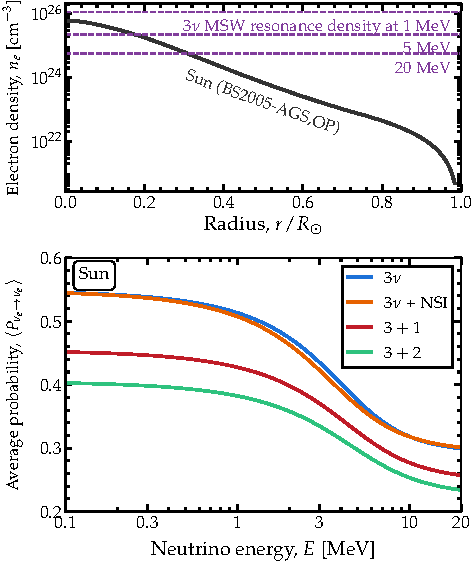
\includegraphics[width=\columnwidth]{solar_averaged.pdf}
 \caption{\label{fig:solar}Phase-averaged survival probability of a solar neutrino, and the density profile that sets it. The neutrino is born at the center of the Sun. {\it Top}: the electron number density along a radial ray of the BS2005-AGS,OP solar model\ \cite{Bahcall:2004pz}. The marked densities are those of the MSW resonance, $\sqrt{2} G_F n_e = \Delta m^2_{21}\cos 2\theta_{12}/2E$, at three energies: a $20$~MeV neutrino crosses it a third of the way out, a $1$~MeV neutrino never does. {\it Bottom}: the phase-averaged survival probability of \equ{averaged_varying}, computed with {\tt average=True} for four Hamiltonians on the same profile. The two sterile cases lie lowest, $3+2$ below $3+1$, because each extra state takes a share of the flux that does not return. Listing~\ref{lst:sun} generates the data. See notebooks \#10, \#13, and \#28, and Sec.~\ref{sec:sun} for details.}
\end{figure}
%%%%%%%%%%%%%%%%%%%%%%%%%%%%%%%%%%%%%%%%%%%%%%%%%%%%%

Figure~\ref{fig:solar} shows the solar electron density from the BS2005-AGS,OP solar model\ \cite{Bahcall:2004pz}, and the averaged survival probability it produces for four Hamiltonians. The Sun needs both the method of Sec.~\ref{sec:method} and the observable of Sec.~\ref{sec:averaged}. Its density falls smoothly by five orders of magnitude along a radial ray, with no discontinuity anywhere to align a slab edge to. A 5-MeV neutrino accumulates a phase of order $10^{6}$ radians on the way out, so its survival probability at the surface runs through a full oscillation when the production point moves by a few kilometers or the energy by a few parts in a million. Neutrinos are produced over a region thousands of times wider than that; no detector resolves energy that finely either. Therefore, what a solar experiment measures is the average probability over the phase, \equ{averaged_varying}, with the eigenbasis of production taken at the center of the Sun and that of detection in vacuum, at its surface.

The energy dependence in the bottom panel of \figu{solar} is set by where the resonance density of the top panel sits relative to the density at production. The resonance density falls with energy as $1/E$. At 1~MeV, it lies above the central density, so the neutrino is born on the vacuum side of the resonance and stays there; its average is the vacuum value, about 0.55. At 20~MeV, the resonance sits a third of the way out. A neutrino born inside it is mostly the matter eigenstate that connects adiabatically to $\nu_2$, so it leaves the Sun as $\nu_2$; its average drops to $\lvert \mathbb{U}_{e2} \rvert^2 \approx 0.3$. 

The bottom panel shows the passage between the two regimes, over an energy range that spans the spectrum of neutrinos from $^8$B decay. Along the ray, the density changes slowly compared with the local oscillation length, so a neutrino stays in the eigenstate it was born in: $P^{\rm cross}$ in \equ{averaged_varying} is the identity, at every energy. What remains are the two eigenbases at the ends of the ray. The one at the surface is the vacuum mixing matrix, the same for any profile; the other end is inside the Sun, with a density given by where the neutrino is born. 

Listing~\ref{lst:sun} computes the four curves. The BS2005-AGS,OP table is one of the twelve standard solar models that ship with \magnus\ (\tabl{solar_models}), and every Sun wrapper takes it by name through {\tt density\_profile}. The wrapper interpolates the electron number density log-linearly between the tabulated radii. For the sterile states, it also reads the neutron-to-proton ratio from the table, $n_n/n_p = (1 - X)/(1 + X)$ at each radius, with $X$ the hydrogen mass fraction. The only difference from an ordinary probability call is {\tt average=True} (Sec.~\ref{sec:average_keyword}). With it, \magnus\ does not propagate along the ray. Instead, it diagonalizes $\mathbb{H}$ at the two ends of the ray, verifies along the ray that the passage is adiabatic and that the levels have decohered by the surface, and contracts the two eigenbases as in \equ{averaged_varying}. Where a crossing fails the adiabatic test, it is bridged by the Magnus patch of Sec.~\ref{sec:hybrid}; on the Sun, none does. 

In Listing~\ref{lst:sun}, between the four probability calls only the wrapper changes, and with it the Hamiltonian. The cost of the calls follows the number of levels whose eigenvalues must be tracked, not the content of the Hamiltonian. The non-standard interactions add no levels to the standard three-flavor case, while each sterile state adds level pairs for the engine to test for adiabaticity and decoherence along the ray: three pairs at three flavors, six at $3+1$, ten at $3+2$. The four curves take about 0.5~s, 0.5~s, 0.8~s, and 1.2~s, respectively, over ninety energies.

%%%%%%%%%%%%%%%%%%%%%%%%%%%%%%%%%%%%%%%%%%%%%%%%%%%%%
\begin{lstlisting}[language=Python, caption={The four averaged solar probabilities of \figu{solar}, complete and runnable as it stands: the BS2005-AGS,OP table\ \cite{Bahcall:2004pz} ships with \magnus, and every Sun wrapper takes it by name through {\tt density\_profile}. The same keywords serve the four wrappers. {\tt average=True} is the whole of the difference from an instantaneous call: it returns \equ{averaged_varying} from the eigenbases at the two ends of the ray, without propagating the phase it would otherwise have to average away. The four curves take about three seconds. Naming {\tt 'B16-GS98'} instead gives the B16-GS98 curve of \figu{solar_models}. See notebooks \#10, \#13, and \#28, and Sec.~\ref{sec:sun} for details.}, label={lst:sun}, float=tbp]
import numpy as np
import magnus.oscprob as oscprob
import magnus.globaldefs as gd
import magnus.solarmodels as solarmodels

# The table ships with Magnus. Its columns are read
# only to plot the density (top panel of Fig. 14)
model = 'BS05-AGS-OP'
r = solarmodels.load_solar_model(model)['r_over_r_sun']
ne_sun = solarmodels.electron_density_profile(model)
ne = ne_sun(r*gd.SUN_RADIUS*gd.UNIT_KM)

# The solar spectrum, 0.1 to 20 MeV
E = np.logspace(-1.0, np.log10(20.0), 90)*gd.UNIT_MEV
osc = gd.load_nufit_params('NuFIT 6.1')

# Shared by the four calls: the model by name, from
# the center to its last row, nu_e to nu_e, the average
R = solarmodels.table_edge(model)
run = dict(nu_i=gd.NUE, nu_f=gd.NUE, average=True,
 density_profile=model)

# Standard three-flavor oscillations
P3 = oscprob.osc_prob_3nu_sun(E, R, 0.0, **osc, **run)

# The same, with non-standard interactions
eps = dict(eps_ee=0.10, eps_em=0.05, eps_mt=0.03)
P3_nsi = oscprob.osc_prob_3nu_sun_nsi(
 E, R, 0.0, **osc, **eps, **run)

# One and two sterile states.  n_n/n_p is read from
# the table; passing ratio_number_neutrons_to_protons
# overrides it
ster = dict(s14=0.10**0.5, s24=0.10**0.5, D41=1.0)
P4 = oscprob.osc_prob_4nu_sun(
 E, R, 0.0, **osc, **ster, **run)
P5 = oscprob.osc_prob_5nu_sun(
 E, R, 0.0, **osc, **ster, s15=0.06**0.5,
 s25=0.06**0.5, D51=1.7, **run)

# P3 = 0.5449 at 0.1 MeV, 0.2993 at 20 MeV
\end{lstlisting}
%%%%%%%%%%%%%%%%%%%%%%%%%%%%%%%%%%%%%%%%%%%%%%%%%%%%%

Without the {\tt average} keyword, the same call returns the instantaneous probability at the surface. That answer is correct but not plottable: over the last few thousand kilometers of the ray, the probability fluctuates over most of [0,1], because the phase changes by thousands of radians across that stretch:
\begin{pysnip}
dL = np.array([0, 50, 100])*gd.UNIT_KM
P = oscprob.osc_prob_3nu_sun(
 5.0*gd.UNIT_MEV, R - dL, 0.0, **osc,
 nu_i=gd.NUE, nu_f=gd.NUE, 
 density_profile=model)
# P = 0.208, 0.773, 0.349 in about 7 s
\end{pysnip}
Asked at the end of the ray and 50 and 100~km inside it, for a 5-MeV neutrino, the three values span most of the unit interval, and the hybrid engine of Sec.~\ref{sec:hybrid} certifies each of them. That is why we do not show it in \figu{solar}. Left at its default, {\tt density\_profile='exp'}, a Sun wrapper uses an exponential fit to the solar density instead of a table (Sec.~\ref{sec:solar_model_comparison}).

%%%%%%%%%%%%%%%%%%%%%%%%%%%%%%%%%%%%%%%%%%%%%%%%%%%%%

\subsubsection{Varying the production point}
\label{sec:sun_production_point}

%%%%%%%%%%%%%%%%%%%%%%%%%%%%%%%%%%%%%%%%%%%%%%%%%%%%%
\begin{figure}[t!]
 \centering
 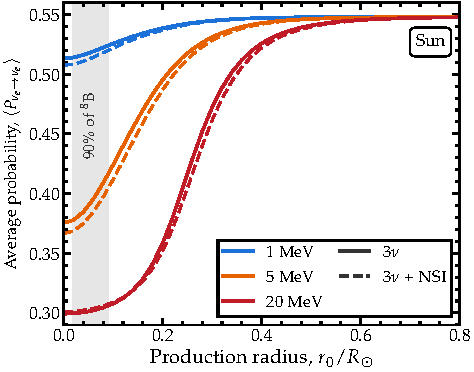
\includegraphics[width=\columnwidth]{solar_production.pdf}
 \caption{\label{fig:solar_production}Phase-averaged survival probability of a solar neutrino as a function of where it is produced, along the radial ray of \figu{solar}, at three energies, with and without the non-standard interactions (NSI) of \figu{solar}. The density is from the BS2005-AGS,OP solar model~\cite{Bahcall:2004pz}. Each curve rises from its value at the center to the vacuum value once the production point lies outside the resonance. The rise is centered on the radius where the resonance density of \figu{solar} meets the profile: a third of the way out at 20~MeV, a sixth at 5~MeV. At 1~MeV, the resonance lies above the central density, so the curve never leaves the vacuum side. The band marks where $90\%$ of the $^8$B neutrinos are made, in the same model. See notebooks \#10, \#13, and \#28, and Sec.~\ref{sec:sun} for details.}
\end{figure}
%%%%%%%%%%%%%%%%%%%%%%%%%%%%%%%%%%%%%%%%%%%%%%%%%%%%%

Figure~\ref{fig:solar_production} takes a different perspective: it moves the production point instead of the energy. At 20~MeV, a neutrino born inside $R_\odot/3$ leaves as $\nu_2$, with the average near $0.3$; born outside, it never meets the resonance and the average is the vacuum value. The step between the two sits at the radius where the resonance line of \figu{solar} crosses the profile; it moves inward as the energy drops, to about $R_\odot/6$ at 5~MeV. At 1~MeV, there is no transition step, since the resonance lies above the central density; what remains is a mild depression. Every point of the figure is one call with {\tt average=True}, like before, and a different {\tt L0}:
\begin{pysnip}
P = oscprob.osc_prob_3nu_sun(
 5.0*gd.UNIT_MEV, R, 
 0.05*gd.SUN_RADIUS*gd.UNIT_KM,
 **osc, **run)
# P = 0.390, against 0.375 from the center
\end{pysnip}
At 5~MeV, moving the production point from the center to where the $^8$B neutrinos are made raises the average by 0.015.

Figure~\ref{fig:solar_production} shows that, given that most $^8$B neutrinos are made around $0.05\,R_\odot$, and given their energies, they are born on the matter side of the resonance. This is why the high-energy end of \figu{solar} sits near 0.3. Non-standard interactions shift each curve by about 0.01, most where the step is. 

%%%%%%%%%%%%%%%%%%%%%%%%%%%%%%%%%%%%%%%%%%%%%%%%%%%%%

\subsubsection{Probability averaging}
\label{sec:averaging_is_not_estimating}

Given a scan of the instantaneous probability at the end of a ray, one might try to reach the averaged observable of \figu{solar} by taking the mean of the scan over its last few oscillation lengths. On the Sun, that mean does not converge. The density keeps falling across the window, and the averaged probability depends on the density, so a wider window averages more of the phase but also more of that change; there is no width at which the two separate. (We tried this in notebook \#13, for a 5-MeV neutrino at two flavors, over the inner tenth of the solar radius. Over the last six oscillation lengths, the mean of the scan is $0.600$; over the last 12, 24, and 48, it lands between $0.599$ and $0.601$. The averaged probability it is meant to estimate is $0.595$, and the mean does not approach it as the window widens.)

The keyword {\tt average=True} takes no window: it evaluates the limit directly from the eigenbases at the two ends of the ray, as described in Sec.~\ref{sec:averaged}. At two flavors on the BS2005-AGS,OP profile, where the textbook expression $\langle P_{\nu_e \to \nu_e}\rangle = \tfrac12 + \tfrac12\cos2\theta_m(l_0)\cos2\theta_m(l_1)$ holds exactly because the passage is adiabatic, with $\theta_m$ the mixing angle in matter at the two ends of the ray, the keyword reproduces it to machine precision across $1$--$20$~MeV.

A scan along the ray has a second problem, and \magnus\ measures it on request. The scan samples an oscillation, and with fewer than two baselines per cycle it is aliased: each value is correct on its own, but a curve drawn through them is not the probability. When {\tt strategy\_info} is passed, the package reports how many cycles the trajectory holds and how many baselines a scan would need to resolve them. The averaged call fills the same report at no cost, since it runs no scan:
\begin{pysnip}
info = {}
P = oscprob.osc_prob_3nu_sun(
 5.0*gd.UNIT_MEV, R, 0.0, **osc,
 strategy_info=info, **run)
s = info['sampling']
s['cycles_over_trajectory']   # 138513.2
s['nyquist_points']           # 277028
\end{pysnip}
Between the center and the surface, the fastest pair of a 5-MeV neutrino goes through $138\,000$ cycles, and a scan that resolved them would need $277\,000$ baselines. On an Earth chord (Sec.~\ref{sec:prem}), the count is a few hundred; on a supernova ray (Sec.~\ref{sec:shock}), tens of thousands. The report is never turned into a warning, deliberately: nearly every realistic scan size fails the criterion, and a warning that fires on nearly every call is noise that users would learn to silence, together with the discontinuity warnings that share its category.

%%%%%%%%%%%%%%%%%%%%%%%%%%%%%%%%%%%%%%%%%%%%%%%%%%%%%

\subsubsection{Comparing against approximations}
\label{sec:sun_compare_approx}

%%%%%%%%%%%%%%%%%%%%%%%%%%%%%%%%%%%%%%%%%%%%%%%%%%%%%
\begin{figure}[t!]
 \centering
 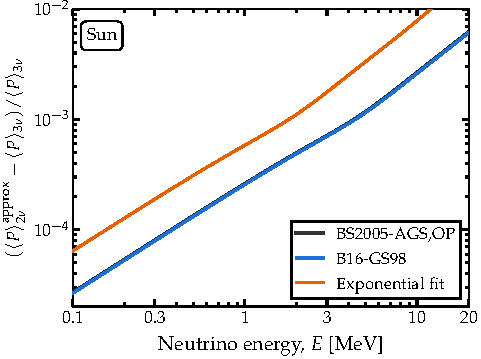
\includegraphics[width=\columnwidth]{solar_approx.pdf}
 \caption{\label{fig:solar_approx}Relative error of the two-flavor approximation to the averaged solar survival probability, $\langle P \rangle^{\rm approx}_{2\nu}$ of \equ{two_flavor_reduction}, with respect to the three-flavor result computed with \magnus, $\langle P \rangle_{3\nu}$, on the three solar density profiles of \figu{solar_models}. The approximation overestimates the probability at every energy, by an amount that grows in proportion to the energy. On the two tabulated models it reaches $0.6\%$ at $20$~MeV. On the exponential fit, whose central density is $2.4$ times higher, it is two to three times larger, and its curve leaves the panel above $10$~MeV. See notebook \#28 and Sec.~\ref{sec:sun_compare_approx} for details.}
\end{figure}
%%%%%%%%%%%%%%%%%%%%%%%%%%%%%%%%%%%%%%%%%%%%%%%%%%%%%

Solar analyses rarely solve the three-flavor problem. The standard shortcut\ \cite{Kuo:1989qe} reduces it to two flavors in two steps. First, the $1$--$2$ sector is solved on its own, as a two-flavor problem with $\theta_{12}$ and $\Delta m^2_{21}$, on an electron density scaled by $\cos^2\theta_{13}$. Second, $\theta_{13}$ is folded back in through
\begin{equation}
 \label{equ:two_flavor_reduction}
 \langle P_{\nu_e \to \nu_e} \rangle
 \simeq
 \langle P \rangle^{\rm approx}_{2\nu}
 \equiv
 \sin^4\theta_{13} + \cos^4\theta_{13}\,\langle P^{2\nu}_{\nu_e \to \nu_e} \rangle \;.
\end{equation}
The reduction rests on $\Delta m^2_{31}$ being large compared with $\Delta m^2_{21}$ and with the matter potential, so that the third mass state decouples. In vacuum, \equ{two_flavor_reduction} is exact. In matter, it drops terms of relative size $2 E V_{\rm CC}/\Delta m^2_{31}$, about $0.1$ at the center of the Sun for a $20$~MeV neutrino, multiplying the admixture $\sin^2\theta_{13} \approx 0.02$ of the decoupled state. Analyses that use the reduction state that these terms are negligible; few evaluate them.

Figure~\ref{fig:solar_approx} evaluates them on the three density profiles of \figu{solar_models}. The three-flavor result, $\langle P \rangle_{3\nu}$, is the numerical result of \magnus: {\tt P3} of Listing~\ref{lst:sun} for the BS2005-AGS,OP table, and the same call on the other two profiles. The two-flavor result needs the density itself, to rescale it, so it takes the profile the wrappers build from the table and goes through the scenario function, which accepts any profile:
\begin{pysnip}
# The 1-2 sector on the rescaled density
c13 = 1.0 - osc['s13']**2
P2 = oscprob.osc_prob_matter_std_potential(
 2, lambda l: c13*ne_sun(l), E, R,
 dict(sth=osc['s12'], Dm2=osc['D21']),
 L0=0.0, nu_i=gd.NUE, nu_f=gd.NUE, average=True,
 density_is_of_number_of_electrons=True)
# Fold theta_13 back in
P_approx = osc['s13']**4 + c13**2*P2
(P_approx - P3)/P3   # 6e-3 at 20 MeV
\end{pysnip}
The approximation overestimates the probability at every energy, on every profile, and its relative error grows in proportion to the energy, as the size of the dropped terms does. On the two tabulated models, which agree here as they did in \figu{solar_models}, it is a few parts in $10^{5}$ at $0.1$~MeV, a few parts in $10^{4}$ at $1$~MeV, and $0.6\%$ at $20$~MeV. On the exponential fit it is two to three times larger, $2\%$ at $20$~MeV, because the fit's central density is $2.4$ times higher and the dropped terms grow with it.

%%%%%%%%%%%%%%%%%%%%%%%%%%%%%%%%%%%%%%%%%%%%%%%%%%%%%

\subsubsection{Comparing solar models}
\label{sec:solar_model_comparison}

%%%%%%%%%%%%%%%%%%%%%%%%%%%%%%%%%%%%%%%%%%%%%%%%%%%%%
{\def\arraystretch{1.2}
\begin{table}[t!]
 {\small
 \begin{tabular}{@{}lp{5.9cm}@{}}
 {\tt density\_profile} & Solar density profile \\
 \hline
 {\tt 'exp'} & Exponential fit~\cite{Giunti:2007ry}; the default \\
 {\tt 'BP2000'} & BP2000~\cite{Bahcall:2000nu}; to $0.95\,R_\odot$ \\
 {\tt 'BP04'} & BP04~\cite{Bahcall:2004fg}; to $0.95\,R_\odot$ \\
 {\tt 'BS05-OP'} & BS2005, GS98 composition~\cite{Bahcall:2004pz}; to $0.98\,R_\odot$ \\
 {\tt 'BS05-AGS-OP'} & BS2005, AGS05 composition~\cite{Bahcall:2004pz}; to $0.98\,R_\odot$ \\
 {\tt 'B16-GS98'} & B16, GS98 composition~\cite{Vinyoles:2016djt} \\
 {\tt 'B16-AGSS09met'} & B16, AGSS09met composition~\cite{Vinyoles:2016djt} \\
 {\tt 'B23-GS98'} & B23, GS98 composition~\cite{Herrera:2023b23} \\
 {\tt 'B23-AGSS09'} & B23, AGSS09 composition~\cite{Herrera:2023b23} \\
 {\tt 'B23-C11'} & B23, C11 composition~\cite{Herrera:2023b23} \\
 {\tt 'B23-AAG21'} & B23, AAG21 composition~\cite{Herrera:2023b23} \\
 {\tt 'B23-MB22m'} & B23, MB22 meteoritic composition~\cite{Herrera:2023b23} \\
 {\tt 'B23-MB22p'} & B23, MB22 photospheric composition~\cite{Herrera:2023b23} \\
 \end{tabular}}
 \caption{\label{tab:solar_models}The solar density profiles that every Sun wrapper takes through {\tt density\_profile}. The  tabulated standard solar models ship with \magnus. The B16 and B23 tables reach the surface; past the last row of the older models, the density continues along the slope of the last tabulated interval, unless {\tt stop\_at\_table\_edge=True}, which returns no probability there. With sterile states, $n_n/n_p$ is read from the same table, unless overridden with {\tt ratio\_number\_neutrons\_to\_protons}. The solar compositions are GS98~\cite{Grevesse:1998bj}, AGS05~\cite{Asplund:2004eu}, AGSS09~\cite{Asplund:2009fu}, C11~\cite{Caffau:2010qc}, AAG21~\cite{Asplund:2021aag}, and MB22~\cite{Magg:2022rxb}. See notebook \#13 and Sec.~\ref{sec:solar_model_comparison} for details.}
\end{table}}
%%%%%%%%%%%%%%%%%%%%%%%%%%%%%%%%%%%%%%%%%%%%%%%%%%%%%

%%%%%%%%%%%%%%%%%%%%%%%%%%%%%%%%%%%%%%%%%%%%%%%%%%%%%
\begin{figure}[t!]
 \centering
 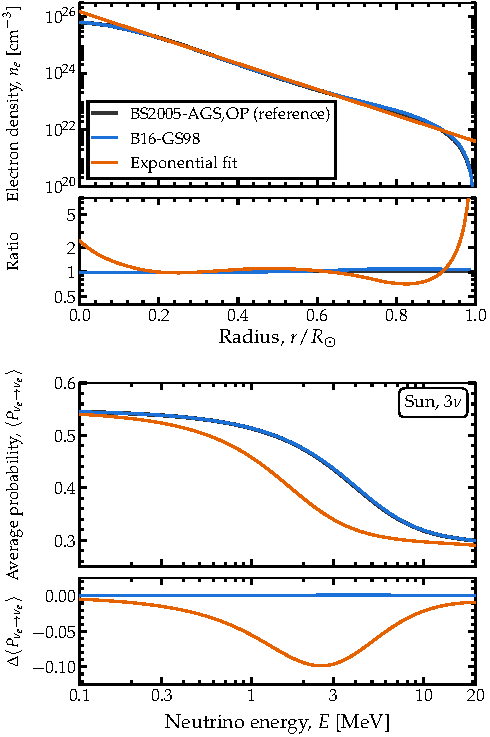
\includegraphics[width=\columnwidth]{solar_models.pdf}
 \caption{\label{fig:solar_models}Three descriptions of the solar electron density, and the averaged survival probability each produces. {\it Top}: the tabulated BS2005-AGS,OP\ \cite{Bahcall:2004pz} and B16-GS98\ \cite{Vinyoles:2016djt} standard solar models, and the exponential fit $n_e = 245\,N_A\,e^{-10.54\,r/R_\odot}$~cm$^{-3}$\ \cite{Giunti:2007ry}, with $N_A$ the Avogadro number, that "that the Sun wrappers use by default, with the ratio of each to BS2005-AGS,OP underneath. The two tables agree to within a few percent; the fit is more than twice too dense at the center and several times too dense in the outermost layers. {\it Bottom}: $\langle P_{\nu_e \to \nu_e}\rangle$ at three flavors on each profile, with the difference from the BS2005-AGS,OP result underneath. The two tables give the same probability to about $10^{-3}$; the fit is low by up to $0.1$, in the middle of the $^8$B spectrum. See notebooks \#10, \#13, and \#28, and Sec.~\ref{sec:sun} for details.}
\end{figure}
%%%%%%%%%%%%%%%%%%%%%%%%%%%%%%%%%%%%%%%%%%%%%%%%%%%%%

\tabl{solar_models} shows the solar density profiles that every Sun wrapper accepts through {\tt density\_profile}. Besides the exponential fit, which is the default, \magnus\ ships twelve tabulated standard solar models from five series published between 2001 and 2023, several of them in more than one solar composition. Each is selected by name, in any case, \eg, {\tt density\_profile='B16-GS98'}. 

From the tabulated mass density, $\rho$, and hydrogen mass fraction, $X$, the wrapper builds the electron number density, $n_e = \rho\,(1 + X)/(2 m_N)$, with $m_N$ the mean nucleon mass, and interpolates it log-linearly in radius. Below the first tabulated radius, it holds the density at its first value, since the core is flat. Past the last one, which lies at $0.95\,R_\odot$ for BP2000 and BP04 and at $0.98\,R_\odot$ for BS2005, it continues the density along the logarithmic slope of the last tabulated interval; passing {\tt stop\us at\us table\us edge=True} returns {\tt NaN} there instead, with a warning. With sterile states, the wrapper reads $n_n/n_p = (1 - X)/(1 + X)$ from the same table. In notebook \#13, we compare all twelve models: they give the same averaged $\nu_e$ survival probability to within $2.4 \cdot 10^{-3}$, and most of that spread separates the series of models rather than the compositions within one series.

Figure~\ref{fig:solar_models} compares the probabilities computed with three choices of solar density profile. Two are tabulated standard solar models, created a decade apart: BS2005-AGS,OP\ \cite{Bahcall:2004pz}, from 2004, used throughout this section, and B16-GS98\ \cite{Vinyoles:2016djt}, from 2016, with updated nuclear rates, equation of state, and opacities. The third is the exponential fit that textbooks quote\ \cite{Giunti:2007ry} and that the Sun wrappers use by default. The two tables track each other to within a few percent over the inner half of the Sun and within ten percent over the outer half. The exponential fit is high by a factor of 2.4 at the center, where the real profile flattens, and high again by several times near the surface of the Sun, where the real profile plunges.

The two solar models give the same averaged probability to about $10^{-3}$ at every energy, far below the precision of any solar measurement. The fit is low by up to 0.1 at a few MeV. The reason is in Sec.~\ref{sec:sun}: on an adiabatic passage, the averaged probability depends on the eigenbases at the two ends of the ray, and the far end is vacuum. What the Sun contributes is the density at the production point, which is exactly where the fit is worst. A profile more than twice too dense at the center moves the transition between the two regimes of \figu{solar} to energies lower by about the same factor. The two plateaus do not move: at low energy, the matter term is negligible for any profile; and at high energy, any profile dense enough at the center places the neutrino above the resonance. A curve shifted sideways between fixed plateaus differs most from the original where it is steepest, at a few MeV, which is where the probabilities differ.

%%%%%%%%%%%%%%%%%%%%%%%%%%%%%%%%%%%%%%%%%%%%%%%%%%%%%

\subsection{A supernova shock front}
\label{sec:shock}

%%%%%%%%%%%%%%%%%%%%%%%%%%%%%%%%%%%%%%%%%%%%%%%%%%%%%
\begin{figure*}[t!]
 \centering
 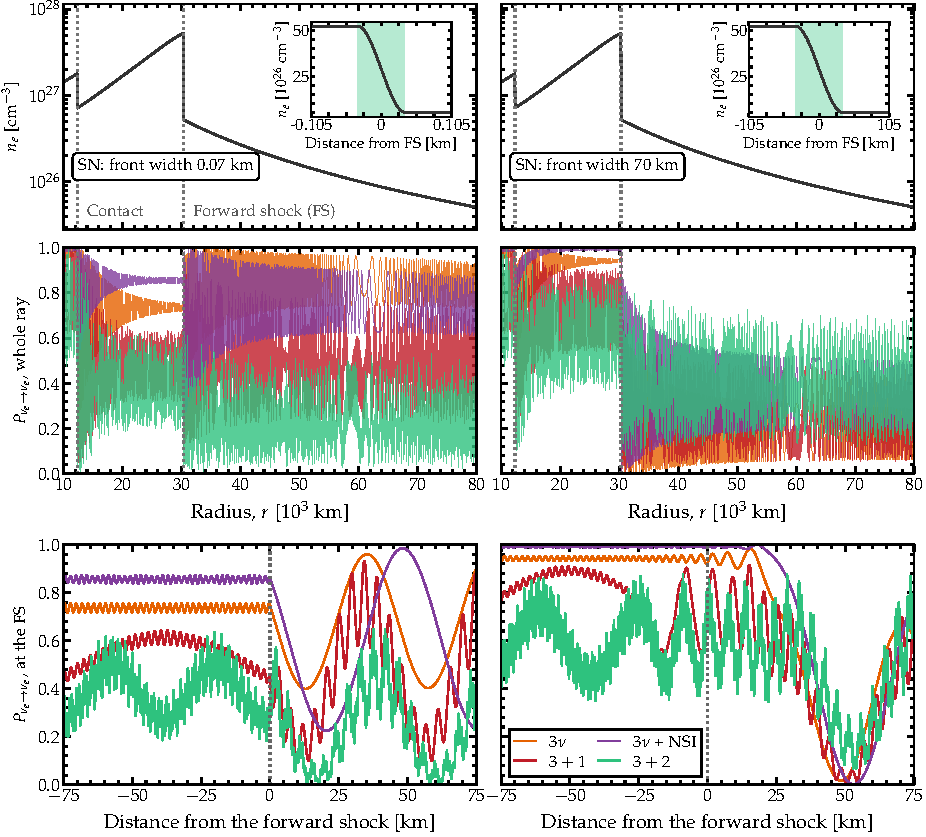
\includegraphics[width=\textwidth]{shock_probability.pdf}
 \caption{\label{fig:shock}Electron number density along a supernova ray, and the survival probability of a $15$-MeV $\nu_e$ along it. {\it Top}: the density from $10^{4}$ to $8 \cdot 10^{4}$~km. Two fronts sit on the ray: the forward shock at $30\,323$~km, where the density jumps by a factor of ten, and the contact discontinuity at $12\,348$~km, where it jumps by $2.5$. The two columns differ in one thing only, the width of both fronts: $0.07$~km on the left, $70$~km on the right. Neither width is visible on the scale of the ray, so the insets show the forward shock, with its extent shaded. {\it Center}: the probability along the whole ray, computed with \magnus\ at ${\tt rtol} = 10^{-8}$ for four Hamiltonians. The ray holds thousands of oscillation lengths of the pair split by $\Delta m^2_{31}$, so the panel resolves the envelope of the oscillation and not the oscillation itself. The two columns agree bitwise up to the contact discontinuity and part there. {\it Bottom}: the same probability through a $\pm 75$~km window at the forward shock, where the oscillation is resolved. Two flavors are not drawn: on $\Delta m^2_{21}$ alone the probability stays between $0.998$ and $1$ at this energy. The profile follows \cite{Schirato:2002tg, Fogli:2003dw}, with the radii of a simulation snapshot\ \cite{Kneller:2014oea}. Listing~\ref{lst:shock} generates the three-flavor curve of the left column. See notebooks \#14 and \#28, and Sec.~\ref{sec:shock} for details.}
\end{figure*}
%%%%%%%%%%%%%%%%%%%%%%%%%%%%%%%%%%%%%%%%%%%%%%%%%%%%%

Figure~\ref{fig:shock} shows a supernova ray, the survival probability of a $15$-MeV neutrino along it, and the same probability resolved at the shock front, for two front widths that differ by a factor of a thousand and in nothing else. The forward shock is the blast wave of the explosion, launched at core bounce and sweeping outward through the envelope: ahead of it the star is still undisturbed, with a density falling as $r^{-2.4}$, and behind it the matter it has swept up is compressed tenfold. The contact discontinuity, inside it, is the surface between that swept-up shell and the ejecta driving the shock from within; across it the pressure is continuous and the density is not. A neutrino leaving the core crosses the contact first, where the density drops by $2.5$, then the shocked shell, thinned by a rarefaction, then the forward shock, where the density drops tenfold. A shock sweeping outward changes the adiabaticity of a level crossing; the change leaves a signature in the neutrino signal\ \cite{Schirato:2002tg, Fogli:2003dw}. This ray carries two such crossings.

What the width of a front does is decided by the oscillation length at the front. The pair split by $\Delta m^2_{21}$ takes no part: at the densities on the ray, near $10^{27}$~cm$^{-3}$, the matter potential is fifty times its vacuum splitting, so that pair is pinned and two flavors barely oscillate here. The pair split by $\Delta m^2_{31}$ does take part, since the potential is comparable to its vacuum splitting, and its oscillation length is about 15~km at 15~MeV. A 0.07-km front is a small fraction of that length: the neutrino crosses it before its state can respond and arrives on the far side as a superposition of the new eigenstates. A 70-km front is a few oscillation lengths wide: the state follows the eigenstates as they rotate and stays in one of them. What changes between the columns is therefore the conversion probability itself, not the phase of an oscillation. At three flavors, the sharp fronts leave a mean survival near 0.8 beyond the forward shock and the wide ones near 0.2. The other Hamiltonians move by different amounts, the 3+2 case in the opposite direction. Each curve is the same call with a different Hermitian matrix.

Listing~\ref{lst:shock} computes the three-flavor curve of the left column. Called without {\tt t\_breakpoints}, the same scan comes out wrong beyond the forward shock, by up to 0.25 in the probability, and \magnus\ says so:
\begin{pysnip}
P = oscprob.osc_prob_matter_std_potential(
 3, ne_shock, 15.0*gd.UNIT_MEV, Ls, osc,
 L0=10000.0*gd.UNIT_KM, rtol=1.0e-8,
 atol=1.0e-10, nu_i=gd.NUE, nu_f=gd.NUE,
 density_is_of_number_of_electrons=True)
# UnmarkedDiscontinuityWarning: the
# Hamiltonian is discontinuous at the scale
# of the grid this scan builds, and no
# t_breakpoints were given.  A slab
# straddling a density jump degrades the
# quadrature no matter how many slabs are
# used; pass t_breakpoints at the
# discontinuities.
\end{pysnip}
Two tolerance warnings come with it, since the ladder ran out of slabs before it could certify the scan. A 0.07-km front lies between two nodes of whatever grid the ladder reaches, and a slab that straddles a jump degrades the quadrature however many slabs are used. The cure is to declare both fronts, as the positions where each begins and ends, so that slab edges fall there at every level of the ladder. That is the difference between the call above and Listing~\ref{lst:shock}. 

A scan of baselines at one energy goes to the cumulative engine, and declared breakpoints keep the adiabatic strategy of Sec.~\ref{sec:hybrid} out of the way in any case; the last line of the listing confirms which engine answered. Notebook \#14 checks the front against an independent integration; notebook \#18 collects the profiles that break a fixed grid. Section~\ref{sec:shock_comparison} measures what the width of the front costs.

%%%%%%%%%%%%%%%%%%%%%%%%%%%%%%%%%%%%%%%%%%%%%%%%%%%%%
\begin{lstlisting}[language=Python, caption={The three-flavor curve of the left column of \figu{shock}: a scan of $4\,000$ baselines along the ray at one energy, with both fronts declared. {\tt t\_breakpoints} names the positions where each front begins and ends, and the refinement puts slab edges there at every level. It is not {\tt t\_slab\_edges}, which replaces the grid instead of seeding it. {\tt ne\_shock} is the electron density of \figu{shock} as a function of position and {\tt osc} the oscillation parameters; both are built in notebook \#14. See Sec.~\ref{sec:shock} for details.}, label={lst:shock}, float=tbp]
import numpy as np
import magnus.oscprob as oscprob
import magnus.globaldefs as gd

# Both fronts, 0.07 km wide, centered on the contact
# discontinuity and on the forward shock: declare
# where each begins and ends
w = 0.07*gd.UNIT_KM
edges = [r + s*w/2 for r in (12348.0*gd.UNIT_KM,
 30323.0*gd.UNIT_KM) for s in (-1.0, 1.0)]

# 4000 baselines from 10,200 to 80,000 km, at one
# energy: the cumulative engine answers
Ls = np.linspace(10200.0, 80000.0, 4000)*gd.UNIT_KM
info = {}
P = oscprob.osc_prob_matter_std_potential(
 3, ne_shock, 15.0*gd.UNIT_MEV, Ls, osc,
 L0=10000.0*gd.UNIT_KM, t_breakpoints=edges,
 rtol=1.0e-8, atol=1.0e-10, strategy_info=info,
 nu_i=gd.NUE, nu_f=gd.NUE,
 density_is_of_number_of_electrons=True)
info['engine']   # 'cumulative'
\end{lstlisting}
%%%%%%%%%%%%%%%%%%%%%%%%%%%%%%%%%%%%%%%%%%%%%%%%%%%%%

A detector measures the survival probability averaged over its energy resolution. Two phases average out inside that resolution. One is the phase accumulated from the forward shock to the detector, hundreds to thousands of cycles at these energies. The other is the phase accumulated between the two fronts: a neutrino can change eigenstate at either crossing, so the two paths interfere, with an interference that cycles about once every ten keV of energy. In the Sun, \equ{averaged_varying} needed only the eigenbases at the two ends of the ray, since the passage was adiabatic with $P^{\rm cross}$ the identity. Here each front is crossed suddenly, so $P^{\rm cross}$ depends on the width of the front; with two crossings, the amplitudes of the two paths add before the modulus is taken. That sum carries the second phase. 

Without the fronts declared, {\tt average=True} still finds the 70-km fronts: it returns 0.37, within the error of the $0.35 \pm 0.04$ that the same call gives with those fronts declared. No probe grid resolves the 0.07-km fronts; there the call returns 0.04, the value for a ray with no fronts at all, against the 0.56 below, and raises {\tt UnmarkedDiscontinuityWarning}, which names the cure. Thus, the correct call to make is with {\tt average=True} and the fronts declared:
\begin{pysnip}
P = oscprob.osc_prob_matter_std_potential(
 3, ne_shock, 15.0*gd.UNIT_MEV, Ls[-1], osc,
 L0=10000.0*gd.UNIT_KM, t_breakpoints=edges,
 average=True, nu_i=gd.NUE, nu_f=gd.NUE,
 density_is_of_number_of_electrons=True)
# PhaseAveragingWarning: average=True on a
# profile with discontinuities has no closed
# form, so the probability was propagated
# across an energy window of +/-10.0% and
# averaged over 41 samples.  This is the
# average over that window, not the L/E ->
# infinity limit, and it depends on the
# window: the largest standard error of the
# mean here is 4.47e-02.  Pass an explicit
# width via magnus.avgprob.
# averaged_probabilities_numerically if
# the measurement has a known resolution.
# P = 0.56
\end{pysnip}
The warning states what \magnus\ did. The two numbers in it are the defaults of {\tt magnus.avgprob}, named constants with their reasons in their docstrings: a half-width of $10\%$, the order of the energy resolution of a detector, which is what does the averaging in a measurement; and $41$ samples, spread evenly in $1/E$ so that they are spread evenly in phase, which put the error of the mean at a few percent, since each sample is a full propagation and the error falls only as the inverse square root of their number. Here that error is $0.04$. A user with a known resolution passes it in place of the default.

%%%%%%%%%%%%%%%%%%%%%%%%%%%%%%%%%%%%%%%%%%%%%%%%%%%%%
\begin{figure}[t!]
 \centering
 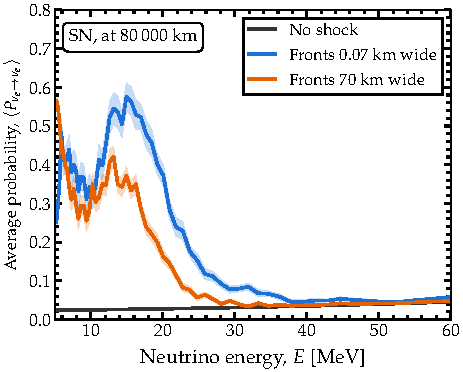
\includegraphics[width=\columnwidth]{shock_energy.pdf}
 \caption{\label{fig:shock_energy}Phase-averaged survival probability of a $\nu_e$ at the end of the supernova ray of \figu{shock}, $80\,000$~km, against energy, with no shock and with the two front widths of that figure. Each point with a shock is the mean over an energy window of $\pm 10\%$, the average that {\tt average=True} returns on a profile with declared fronts; the bands are the standard errors of those means. Without a shock the passage is adiabatic and the survival stays at a few percent. With the fronts it rises to several tenths where the resonance of the pair split by $\Delta m^2_{31}$ sits inside the shocked shell, and returns to the no-shock value above $30$~MeV, where the resonance lies in undisturbed matter beyond the forward shock. See notebooks \#14 and \#28, and Sec.~\ref{sec:shock} for details.}
\end{figure}
%%%%%%%%%%%%%%%%%%%%%%%%%%%%%%%%%%%%%%%%%%%%%%%%%%%%%

Figure~\ref{fig:shock_energy} shows what the shock does to the energy spectrum. Without a shock, the survival probability is a few percent at every energy: the profile is smooth, so the passage is adiabatic and a $\nu_e$ leaves as $\nu_3$. With a shock, the survival rises to tens of percent between about 5 and 25~MeV, and falls back to the no-shock value above 30~MeV. That window is set by where the resonance density, a quantity that scales as $1/E$, falls on the profile. Above 30~MeV, it lies below the density on both sides of the forward shock, so the neutrino crosses it in the smooth matter outside, adiabatically. Between 6 and 25~MeV, it lies between the two sides of the forward shock, so the neutrino crosses it at the front in one step; the state is left in a superposition richer in $\nu_e$. Within that window, the sharp front gives the larger effect, because a 70~km ramp exceeds the oscillation length there, 10--25~km; the state partly follows it. Near 5~MeV, the resonance density also falls between the two sides of the contact discontinuity, so both fronts act. The outcome depends on both crossings and on the phase between them; there, the wide fronts give the larger survival.

%%%%%%%%%%%%%%%%%%%%%%%%%%%%%%%%%%%%%%%%%%%%%%%%%%%%%

\subsection{High-energy astrophysical neutrinos}
\label{sec:astro}

%%%%%%%%%%%%%%%%%%%%%%%%%%%%%%%%%%%%%%%%%%%%%%%%%%%%%
\begin{figure*}[t!]
 \centering
 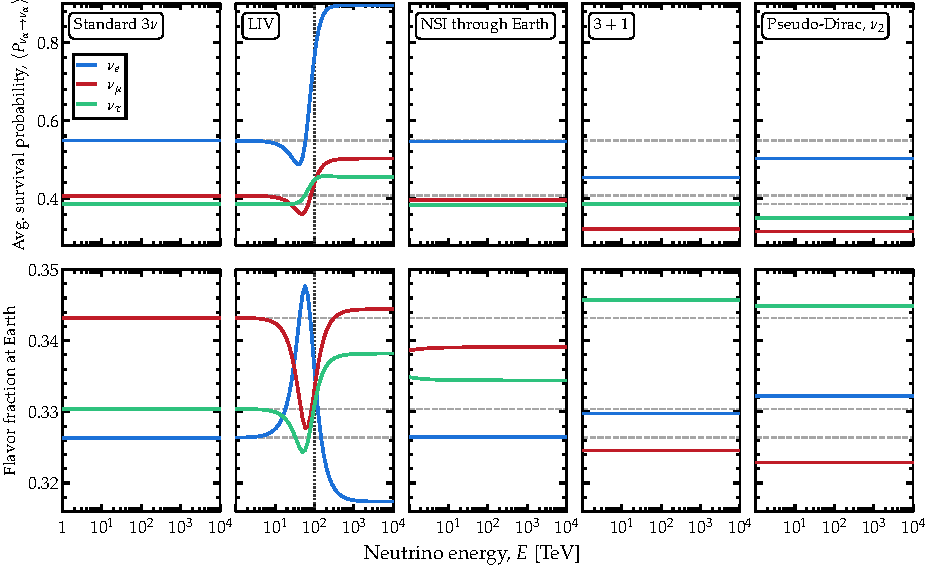
\includegraphics[width=\textwidth]{astro_composition.pdf}
  \caption{\label{fig:astro}Flavor composition of an astrophysical neutrino flux at Earth and the survival probabilities behind it, for five Hamiltonians. Such a flux arrives decohered, so these panels carry the phase-averaged limit of \equ{averaged}, not a propagated probability. \emph{Top}: $\langle P_{\nu_\alpha \to \nu_\alpha}\rangle$ against energy. \emph{Bottom}: the flavor fractions reaching Earth from a pion-decay source, $1:2:0$, with the standard case repeated beneath each panel so that a departure from it is legible. The parameters of the four departures are as follows. Lorentz-invariance violation: the operator of \equ{h_liv_3nu} with $n_{\rm LIV} = 1$, $\Lambda = 1$~eV, eigenvalues $b_1 = b_2 = 0$ and $b_3 = 1.26 \cdot 10^{-31}$~eV, and $\mathbb{V}_\xi$ the PMNS matrix with $\delta_\xi = 0$; the eigenvalue is fixed by asking the new term to equal the vacuum one at 100~TeV; the vertical line marks that energy. Non-standard interactions: $\varepsilon_{ee} = 0.10$, $\varepsilon_{e\mu} = 0.05$ and $\varepsilon_{\mu\tau} = 0.03$, on a chord through the core, $\cos\theta_z = -1$. Sterile state: $\sin^2\theta_{14} = \sin^2\theta_{24} = 0.1$, $\theta_{34} = 0$ and $\Delta m^2_{41} = 1$~eV$^2$. Pseudo-Dirac: the mass eigenstate state $\nu_2$ alone carries a partner, split from it by $\delta m^2 = 10^{-13}$~eV$^2$, at a distance of 100~Mpc. We renormalize the $3+1$ and pseudo-Dirac fractions to the three active flavors, past the 13.3\% and 19.3\% of the flux their sterile states remove, since that share is not observed. Pairing all three mass states would halve every active-active probability by the same factor and leave the fractions untouched, so it is the uneven suppression that moves them. Listing~\ref{lst:astro} computes the five cases. See notebooks \#10, \#13, and \#28 for details, and Sec.~\ref{sec:astro} for details.}
\end{figure*}
%%%%%%%%%%%%%%%%%%%%%%%%%%%%%%%%%%%%%%%%%%%%%%%%%%%%%

Figure~\ref{fig:astro} shows the flavor composition of a TeV--PeV astrophysical flux at Earth and the average flavor-transition probabilities behind it, for five Hamiltonians: standard three-flavor, Lorentz-invariance violation (LIV), non-standard interactions (NSI) through the Earth, $3+1$ flavors, and pseudo-Dirac neutrinos with the $\nu_2$ mass eigenstate split. The top row carries the survival probabilities $\langle P_{\nu_\alpha \to \nu_\alpha}\rangle$; the bottom row, the flavor fractions reaching Earth from a source that produces neutrinos through the full pion decay chain, described next.

\smallskip

\textit{Producing them.}---In cosmic accelerators---active galaxies, gamma-ray bursts, superluminous supernovae---protons may interact with ambient matter and radiation to produce pions\ \cite{Margolis:1977wt, Stecker:1978ah, Kelner:2006tc}. The pions decay via $\pi^+ \to \mu^+ + \nu_\mu$, followed by $\mu^+ \to \bar{\nu}_\mu + \nu_e + e^+$, and their charge conjugates, so that the flux leaving the source carries flavor ratios $(f_e, f_\mu, f_\tau)_{\rm S} = \left(\frac{1}{3}, \frac{2}{3}, 0\right)$, with $f_{\alpha, {\rm S}}$ the fraction of $\nu_\alpha + \bar{\nu}_\alpha$ in the total. Neutrino telescopes cannot ordinarily tell $\nu$ from $\bar\nu$, so $\nu_\alpha$ below means $\nu_\alpha + \bar{\nu}_\alpha$. For illustration, we adopt that full pion-decay composition---the nominal expectation---though other there are other possibilities~(see, \eg, \Ref~\cite{Bustamante:2015waa}). 

\smallskip

\textit{What is observable.}---Over Mpc--Gpc baselines, the oscillation length is minute against the distance; neither the distance, the size of the production region, nor the energy resolution of a detector is known to anything approaching the precision the phase would demand for the oscillations to be resolved. Therefore, a neutrino telescope is sensitive only to the average flavor-transition probabilities $\langle P_{\nu_\alpha \to \nu_\beta}\rangle$ of \equ{averaged}. 

\magnus\ returns the probability in closed form from the eigenvectors of $\mathbb{H}$, with no phase propagated. In vacuum and under standard oscillations, $\mathbb{V}$ in \equ{averaged} is the PMNS matrix, $\mathbb{U}$, and the probability becomes the familiar $\sum_i \lvert U_{\alpha i}\rvert^2 \lvert U_{\beta i}\rvert^2$. In either case, the flavor ratio at Earth is $f_{\alpha, \oplus} = \sum_\beta \langle P_{\nu_\beta \to \nu_\alpha}\rangle f_{\beta, {\rm S}}$. The flavor composition is a rich probe of astrophysics and fundamental physics; see, \eg, \Refs~\cite{Esmaili:2009dz, Barenboim:2003jm, Beacom:2003nh, Kachelriess:2006ksy, Lipari:2007su, Hummer:2010ai, Bustamante:2015waa, Arguelles:2015dca, Rasmussen:2017ert, Bustamante:2019sdb, Ackermann:2019cxh, Ackermann:2019ows, Arguelles:2019rbn, Bustamante:2020bxp, Song:2020nfh, Liu:2023flr}.

Evaluating $\mathbb{U}$ at the NuFIT~6.1 best-fit values of the mixing parameters yields about equal proportion of each flavor at Earth, \ie, $(0.33, 0.34, 0.33)_\oplus$. Oscillation over astrophysical distances populates a $\nu_\tau$ component that the sources do not make. Run backward, the measured flavor composition can be turned into a constraint on the sources\ \cite{Bustamante:2019sdb, Song:2020nfh, Liu:2023flr, IceCube:2025ole}. 

In the presence of mixing with sterile states of or new, non-matter terms added to the \emph{vacuum} Hamiltonian (like Lorentz-invariance violation, which holds in vacuum and in matter), the probability is the same expression as above, but evaluated in the eigenbasis of the total Hamiltonian, \ie, $\sum_i \lvert V_{\alpha i}\rvert^2 \lvert V_{\beta i}\rvert^2$. 

Matter is different: the flux decoheres in the vacuum mass basis long before it arrives, then crosses the Earth \emph{coherently}. Thus, the two legs compose as probability matrices rather than as amplitudes, yielding a flavor ratio at Earth of $f_{\beta,\oplus} = \sum_{\alpha,\gamma} f_{\alpha, {\rm S}} \langle P_{\nu_\alpha \to \nu_\gamma}\rangle P^{\oplus}_{\nu_\gamma \to \nu_\beta}$, with the second factor an ordinary propagation through the Earth's density profile.  

Listing~\ref{lst:astro} computes the five cases of \figu{astro}. Three of them are one wrapper call each with {\tt average=True}, over all energies at once: the standard case, the Lorentz-violating case, and the $3+1$ case. The wrappers decide from the baseline and the eigenvalue gaps which pairs have decohered, so the baseline passed must be astrophysical in fact. At 100~Mpc every pair has decohered at every energy of the figure; over $10^8$~km, less than an astronomical unit, the pair split by $\Delta m^2_{21}$ has not completed a cycle above a few TeV, so the wrapper warns and returns the coherent expression instead. The pseudo-Dirac case has no wrapper: its Hamiltonian is built and handed to the direct route with the baseline, from which the average decides which pairs of eigenvalues have decohered.

Only the Earth leg with non-standard interactions propagates a probability; the other four cases are closed-form averages. That call passes {\tt n\_slabs=32}: on the default first grid a slab spans thousands of km, across which the matter term alone accumulates a phase above $\pi$, the bound below which the expansion is guaranteed to converge. \magnus\ warns about that and refines anyway; starting at 32 slabs removes the warning, with a change in the answer below the tolerance. 

\smallskip

%%%%%%%%%%%%%%%%%%%%%%%%%%%%%%%%%%%%%%%%%%%%%%%%%%%%%
\begin{lstlisting}[language=Python, caption={The five cases of \figu{astro}: the phase-averaged matrix $\langle P_{\nu_\alpha \to \nu_\beta}\rangle$ of \equ{averaged} for each Hamiltonian, over the sixty energies of the figure, contracted with the pion-decay source fractions. The standard, Lorentz-violating and $3+1$ cases are one wrapper call each with {\tt average=True}; the Earth case composes the decohered matrix with one propagation through the core; the pseudo-Dirac case builds its Hamiltonian and takes the direct route with the baseline, from which the average groups the spectrum into coherent blocks. {\tt f\_earth} holds the five compositions. See Sec.~\ref{sec:astro} for details.}, label={lst:astro}, float=tbp]
import numpy as np
import magnus.oscprob as oscprob
import magnus.hamiltonians as ham
import magnus.earth as earth
import magnus.globaldefs as gd

osc = gd.load_nufit_params('NuFIT 6.1')
E = np.logspace(3, 7, 60)*gd.UNIT_GEV   # 1 TeV-10 PeV
f_src = np.array([1/3, 2/3, 0.0])       # pion decay
# A source 100 Mpc away: far enough for every pair
# of eigenvalues to have decohered at every energy,
# which the wrappers decide from the baseline
L_src = 100.0*3.0857e19*gd.UNIT_KM

def at_earth(P):
    # The source fractions, zero for a sterile state,
    # contracted with the averaged matrix; the active
    # fractions renormalized to one
    f = np.zeros(len(P)); f[:3] = f_src
    f = (f @ P)[:3]
    return f/f.sum()

# Standard: the averaged matrix at each energy
P_std = oscprob.osc_prob_3nu_vacuum(E, L_src,
 average=True, **osc)                   # (60, 3, 3)

# LIV: the n = 1 operator, aligned with the PMNS
# angles, sized to equal the vacuum term at 100 TeV
b3 = osc['D31']/(2*(100.0*gd.UNIT_TEV)**2)
P_liv = oscprob.osc_prob_3nu_vacuum_liv(E, L_src,
 average=True, sxi12=osc['s12'], sxi23=osc['s23'],
 sxi13=osc['s13'], dxiCP=0.0, b1=0.0, b2=0.0,
 b3=b3, Lambda=1.0, n_liv=1, **osc)

# NSI through the Earth: the flux arrives decohered,
# then crosses the Earth coherently, so the two legs
# compose as probability matrices.  The ladder starts
# at 32 slabs: the matter term alone winds more than
# pi across a coarser one
eps = dict(eps_ee=0.10, eps_em=0.05, eps_mt=0.03)
L_in = earth.distance_traveled_inside_earth(-1.0)
P_in = oscprob.osc_prob_3nu_earth_nsi(E, costhz=-1.0,
 L=L_in*gd.UNIT_KM, n_slabs=32, rtol=1e-6, atol=1e-8,
 **osc, **eps)
P_nsi = np.asarray(P_std) @ np.asarray(P_in)

# 3+1: one sterile state, sin^2 of both active-
# sterile angles 0.1, Dm41^2 = 1 eV^2
P_4 = oscprob.osc_prob_4nu_vacuum(E, L_src,
 average=True, s14=np.sqrt(0.1), s24=np.sqrt(0.1),
 D41=1.0, **osc)

# Pseudo-Dirac: no wrapper, so the Hamiltonian is
# built and handed to the direct route.  The second
# mass state is paired with a partner split by
# 1e-13 eV^2; the baseline decides which pairs have
# decohered
U = ham.pmns_mixing_matrix(osc['s12'], osc['s23'],
 osc['s13'], osc['dCP'])
m2 = np.array([0.0, osc['D21'], osc['D31']])
def H_pd(e):
    return ham.hamiltonian_pseudo_dirac_vacuum(
     e, U, m2, {1: 1.0e-13})
P_pd = np.array([oscprob.osc_prob_energy_baseline(
 H_pd(e), e, L_src, average=True) for e in E])

cases = dict(std=P_std, liv=P_liv, nsi=P_nsi,
             four=P_4, pd=P_pd)
f_earth = {k: np.array([at_earth(P) for P in v])
           for k, v in cases.items()}
\end{lstlisting}
%%%%%%%%%%%%%%%%%%%%%%%%%%%%%%%%%%%%%%%%%%%%%%%%%%%%%

\textit{What varies with energy, and what does not.}---For standard oscillations the composition does not depend on the energy at all. Equation~(\ref{equ:averaged}) is built from $\lvert \mathbb{V}_{\alpha i}\rvert^2$ alone; in vacuum no energy enters them. Three of the four departures from standard oscillations are flat in energy:
\begin{itemize}
 \item 
  In the $3+1$ case, a sterile state moves the composition at Earth from $(0.326, 0.343, 0.330)_\oplus$ to $(0.330, 0.325, 0.346)_\oplus$. (Sterile states take away 13.3\% of the originally purely active flux; these triplets are the three active fractions rescaled to add to one.)
 \item 
  In NSI through the Earth, the fractions move by less than 0.005 and also do not vary, because above a TeV the matter term dominates the Hamiltonian inside the Earth and carries no energy dependence. (Towards the low energy end, the energy dependence starts becoming visible.)
 \item
  In the pseudo-Dirac case, expanded below, the composition is flat in energy for the same reason as for sterile neutrinos: it is a vacuum Hamiltonian, just with more states.
\end{itemize}
The three cases induce different shifts in $f_{\alpha, \oplus}$, independent of energy within the range shown. Above about 100~TeV, a neutrino crossing the core is likely to interact on the way and never reach the detector, an effect \magnus\ does not account for.

What separates the Lorentz-violating case from the others is that its term keeps growing with energy ($\propto E$) relative to the vacuum one ($\propto 1/E$), so the eigenvectors never settle; the other three cases reach a regime in which one term dominates and the composition stops moving. The Lorentz-violating case moves $f_{e, \oplus}$ from about 0.33 up to 0.35 and down again to 0.32 across the crossover, with $f_{\mu, \oplus}$ dipping to 0.33 and recovering; the survival probability driving it reaches 0.89. That is what a flavor measurement could distinguish; \magnus\ evaluates \equ{averaged} for it in the same call as for the standard case.

%%%%%%%%%%%%%%%%%%%%%%%%%%%%%%%%%%%%%%%%%%%%%%%%%%%%%
\begin{figure}[t!]
 \centering
 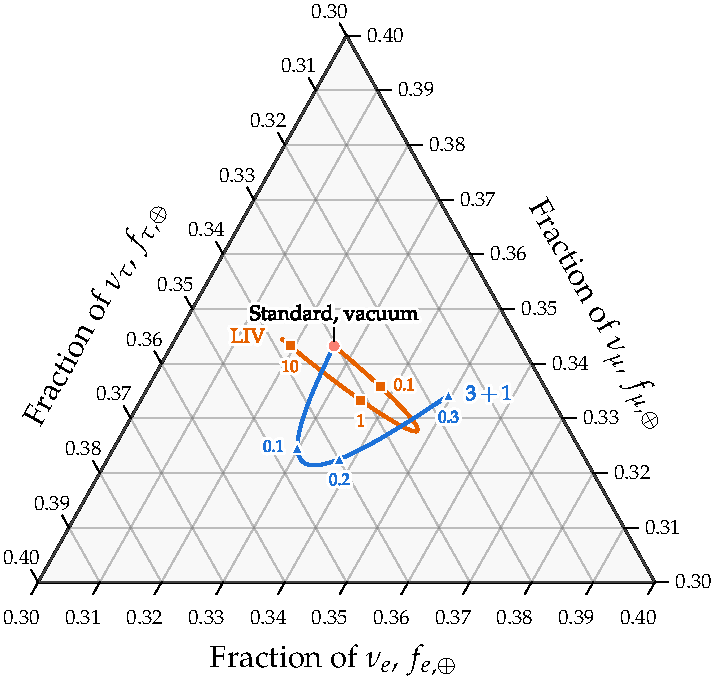
\includegraphics[width=\columnwidth]{astro_ternary.pdf}
 \caption{\label{fig:astro_ternary}Flavor composition at Earth of a pion-decay flux of high-energy astrophysical neutrinos. The flavor composition at the source is $\left(\frac{1}{3}:\frac{2}{3}:0\right)_{\rm S}$. Results are for standard, three-flavor oscillations in vacuum, for Lorentz-invariance violation (LIV), and for active-sterile mixing under 3+1 flavors. The standard expectation is $(0.326, 0.343, 0.330)_\oplus$. Along the LIV curve, the eigenvalue $b_3$ of the $n = 1$ LIV operator of \figu{astro} grows from zero at $E = 100$~TeV; the marks are where the new term is 0.1, 1, and 10 times the vacuum one, the energies 32, 100, and 316~TeV. Along the 3+1 curve, the two active-sterile mixing angles grow together from zero; the marks are $\sin^2\theta_{14} = \sin^2\theta_{24} = 0.1$, 0.2 and 0.3, with flavor fractions renormalized to the active flavors. See notebooks \#10, \#13, and \#28 for details, and Sec.~\ref{sec:astro} for details.}
\end{figure}
%%%%%%%%%%%%%%%%%%%%%%%%%%%%%%%%%%%%%%%%%%%%%%%%%%%%%

Figure~\ref{fig:astro_ternary} shows two of these flavor compositions on the flavor triangle, as their new-physics parameter is varied. Along the LIV curve, the eigenvalue of the Lorentz-violating operator grows from zero at 100~TeV: the composition leaves the standard point, swings out through the crossover and settles where the new term alone puts it, close to where it started. Along the 3+1 curve, the two active-sterile mixing angles grow together from zero; the composition moves the other way. Given the ranges over the model parameters are varied in \figu{astro}, every point lies within a few hundredths of the standard one, so the triangle is drawn over 0.30 to 0.40 on each axis.

\smallskip

\textit{Pseudo-Dirac neutrinos.}---The fifth panel in \figu{astro} splits the mass eigenstate $\nu_2$ into a pair separated by $\delta m^2 = 10^{-13}$~eV$^2$, its partner sterile\ \cite{Wolfenstein:1981kw, Petcov:1982ya} (see Sec.~\ref{sec:shipped_hamiltonians}). Only one of the mass eigenstates is split: splitting all three sends half the flux to the sterile partners and divides every probability between active flavors by 2, so the three flavor fractions a detector sees come out standard. Splitting $\nu_2$ only sends 19.3\% of the flux to its partner and moves the fractions.

Which averaged expression applies to the probability depends on the phase the pair itself accumulates, $\delta m^2 L / 2E$. At 100~Mpc and 100~TeV, below about $10^{-19}$~eV$^2$, that phase is a small fraction of a radian: the pair stays coherent and \equ{averaged_blocks} returns exactly what an unsplit spectrum gives. Above about $10^{-16}$~eV$^2$ the phase turns through more than a cycle: the pair has averaged away and \equ{averaged} counts the two members separately, halving the channels they carry. The figure sits above that band, at $10^{-13}$~eV$^2$. \magnus\ decides which regime a spectrum is in from the eigenvalues and the baseline:
\begin{pysnip}
import magnus.avgprob as avgprob

E1 = 100.0*gd.UNIT_TEV
for dm2 in (1.0e-13, 1.0e-19):
    H = ham.hamiltonian_pseudo_dirac_vacuum(
     E1, U, m2, {1: dm2})
    lam = np.linalg.eigvalsh(H)
    b = avgprob.coherence_blocks(lam, L_src)
    print(b)
# [[0], [1], [2], [3]]   The pair decohered
# [[0], [1, 2], [3]]     The pair coherent
\end{pysnip}
Between the two regimes neither expression describes the situation accurately; passing {\tt average=True} says so instead of returning a number. The signature such a spectrum leaves at a neutrino telescope is the one identified in \Ref\ \cite{Beacom:2003eu}. 

%%%%%%%%%%%%%%%%%%%%%%%%%%%%%%%%%%%%%%%%%%%%%%%%%%%%%

\subsection{Assorted long examples}

%%%%%%%%%%%%%%%%%%%%%%%%%%%%%%%%%%%%%%%%%%%%%%%%%%%%%

\subsubsection{A cavity in the Earth's crust}
\label{sec:cavity}

%%%%%%%%%%%%%%%%%%%%%%%%%%%%%%%%%%%%%%%%%%%%%%%%%%%%%
\begin{figure}[t!]
 \centering
 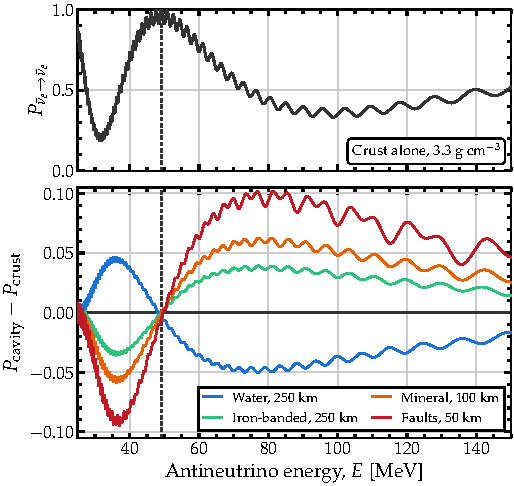
\includegraphics[width=\columnwidth]{cavity.pdf}
 \caption{\label{fig:cavity}Effect of a cavity in the Earth's crust on the $\bar{\nu}_e$ survival probability over a baseline of $1\,500$~km, computed with \magnus, after \Ref\ \cite{Arguelles:2012nw}. {\it Top}: the crust alone, uniform at 3.3~g~cm$^{-3}$ with $Y_e = 0.5$. {\it Bottom}: the change that four cavities make to it, each centered on the baseline, with the density and width its label gives. The water cavity carries $Y_e = 0.555$, the other three 0.5. The dashed line marks 49~MeV, where the crust curve peaks. The beam of \Ref\ \cite{Arguelles:2012nw} spans 5--150~MeV; below 25~MeV, the oscillation is too rapid to draw. Listing~\ref{lst:cavity} computes every curve. See notebook \#28 and Sec.~\ref{sec:cavity} for details.}
\end{figure}
%%%%%%%%%%%%%%%%%%%%%%%%%%%%%%%%%%%%%%%%%%%%%%%%%%%%%

%%%%%%%%%%%%%%%%%%%%%%%%%%%%%%%%%%%%%%%%%%%%%%%%%%%%%
\begin{lstlisting}[language=Python, caption={A cavity search in the Earth's crust, after \Ref\ \cite{Arguelles:2012nw}: the $\bar{\nu}_e$ survival probability over $1\,500$~km of Earth's crust, with and without a cavity of different density centered on the baseline. A cavity is a density profile with two walls, whose positions are declared as breakpoints so that the refinement ladder runs inside the cavity. See Sec.~\ref{sec:cavity} for details.}, label={lst:cavity}, float=tbp]
import numpy as np
import magnus.oscprob as oscprob
import magnus.matter as matter
import magnus.globaldefs as gd

L0 = 1500.0                     # km, source to detector
RHO_CRUST, YE_CRUST = 3.3, 0.5  # PREM crust
E = np.linspace(25.0, 150.0, 2500)*gd.UNIT_MEV
osc = gd.load_nufit_params('NuFIT 6.1')
kw = dict(osc_params=osc, L0=0.0, nu_i=gd.NUE,
          nu_f=gd.NUE, nubar=True, rtol=1.0e-8,
          atol=1.0e-10,
          density_is_of_number_of_electrons=True)

def n_e(rho, ye):
    """Electron density [eV^3] of uniform matter."""
    return matter.num_density_e_func(
        0.0, lambda _: rho, electron_fraction=ye,
        ratio_number_neutrons_to_protons=(1.0-ye)/ye,
        density_matter_is_in_g_per_cm3=True)

NE_CRUST = n_e(RHO_CRUST, YE_CRUST)

def cavity(rho, ye, w):
    """Crust holding a cavity of width w, centered."""
    d = (L0 - w)/2.0
    ne_in = n_e(rho, ye)

    def profile(l):
        x = np.asarray(l, dtype=float)/gd.UNIT_KM
        return NE_CRUST + (ne_in - NE_CRUST) \
            *((x >= d) & (x <= d + w))

    return profile, np.array([d, d + w])*gd.UNIT_KM

# An empty crust needs no profile, only a number
P0 = oscprob.osc_prob_matter_std_potential(
    3, NE_CRUST, E, L0*gd.UNIT_KM, **kw)

# Water, iron, a mineral deposit, a zone of faults:
# (rho, Y_e, w) for each
CASES = [(1.0, 0.555, 250.0), (5.0, 0.5, 250.0),
         (10.0, 0.5, 100.0), (25.0, 0.5, 50.0)]
dP = []
for rho, ye, w in CASES:
    profile, walls = cavity(rho, ye, w)
    # The two walls are density jumps: declare them
    P = oscprob.osc_prob_matter_std_potential(
        3, profile, E, L0*gd.UNIT_KM,
        t_breakpoints=walls, **kw)
    dP.append(P - P0)
\end{lstlisting}
%%%%%%%%%%%%%%%%%%%%%%%%%%%%%%%%%%%%%%%%%%%%%%%%%%%%%

A region of anomalous density along the trajectory of a neutrino moving in an otherwise uniform medium changes the oscillation probability measured at the far end. This observation has motivated proposals for using neutrinos to search for underground cavities in the Earth's crust. We use \magnus\ to implement the prescription of \Ref\ \cite{Arguelles:2012nw}: a low-energy $\bar{\nu}_e$ beam crossing $1\,500$~km of crust, with the survival probability measured from 5 to 150~MeV. Our goal is primarily illustrative; we point out the doubtful feasibility of such an experimental setup.

Listing~\ref{lst:cavity} sets this up in \magnus. The crust is uniform at 3.3~g~cm$^{-3}$ with $Y_e = 0.5$, the average of the outermost PREM layers. The cavity is a slab of different density centered on the baseline. We show cavities of four densities~\cite{Arguelles:2012nw}: water at 1~g~cm$^{-3}$ and $Y_e = 0.555$, an iron-banded formation at 5~g~cm$^{-3}$, a mineral deposit at 10~g~cm$^{-3}$, a zone of seismic faults at 25~g~cm$^{-3}$. Their widths along the neutrino trajectory fall from 250 to 50~km as the contrast with the crust grows. Each cavity has two walls. Every wall is a density jump: we pass their positions via {\tt t\_breakpoints} to the scenario function, allowing the refinement ladder to act inside the cavity.

Figure~\ref{fig:cavity} shows the resulting probabilities. Every cavity curve crosses zero near the $49$~MeV at which the crust curve peaks at 0.9997 (it would be exactly 1 if $\theta_{13}$ were zero). The presence of a cavity moves the peak energy. Adding column density pushes the peak up in energy; removing column density pulls it down. What a cavity does to the curve is to displace it bodily along the energy axis, leaving its shape almost untouched.  For a denser cavity, at energies below the peak the peak has moved further away, so the probability there falls; at energies above the peak it has moved closer, so the probability rises. A lighter cavity moves the peak the other way, swapping both signs. Either way the shift crosses zero between the crust's peak and the cavity's, which puts the four crossings between 48.1 and 49.5~MeV.

Figure~\ref{fig:cavity_sweep} turns the neutrino beam across the cavity. The source stays put and the baseline keeps its length; only the direction changes, by an angle $\alpha$. Each direction cuts a different slice through the same cavity, a sphere of radius 125~km centered 750~km along the baseline. (Reference~\cite{Arguelles:2012nw} works with elliptical cavities, but a sphere carries the point just as well.) The spread of the angle is $\alpha = \pm 9.59^\circ$; within those angles, the cavity width it crosses traces a semicircle.

The probability contrast map reflects that semicircle. Structure fills the $\alpha$ band and fades at its edges as the width falls. Outside the band, the beam misses the body, so the profile is the uniform crust and the difference is exactly zero. The sweep is what separates a large, light body from a small heavy one: a single direction measures only the excess column, in which density and width are degenerate, while the angular width of the band fixes the size by itself. Listing~\ref{lst:cavity_sweep} computes the map.

%%%%%%%%%%%%%%%%%%%%%%%%%%%%%%%%%%%%%%%%%%%%%%%%%%%%%
\begin{figure}[t!]
 \centering
 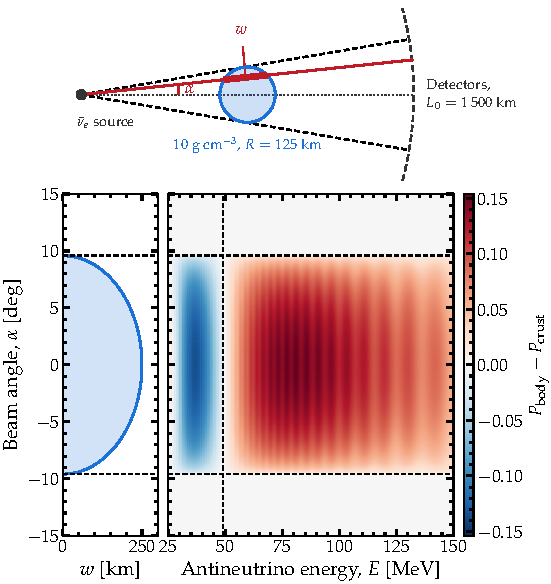
\includegraphics[width=\columnwidth]{cavity_sweep.pdf}
 \caption{\label{fig:cavity_sweep}{\it Top}: the geometry. The beam leaves the source at an angle $\alpha$ and reaches a detector on the dashed arc, $1\,500$~km away. The two dashed straight lines are the beams tangent to the body, at $\alpha = \pm 9.59^\circ$. A neutrino beam crosses the cavity width, $w$. {\it Bottom left}: that width against the angle, \ie, the cavity's silhouette. {\it Bottom right}: the change in probability over energy and angle. The dashed vertical line marks the $49$~MeV of \figu{cavity}. Listing~\ref{lst:cavity_sweep} computes the map.}
\end{figure}
%%%%%%%%%%%%%%%%%%%%%%%%%%%%%%%%%%%%%%%%%%%%%%%%%%%%%

%%%%%%%%%%%%%%%%%%%%%%%%%%%%%%%%%%%%%%%%%%%%%%%%%%%%%
\begin{lstlisting}[language=Python, caption={The map of \figu{cavity_sweep}, continuing Listing~\ref{lst:cavity}, whose {\tt n\_e}, {\tt NE\_CRUST}, {\tt L0} and {\tt kw} it reuses. Only the geometry is new: at each angle, where the chord enters and leaves the body. Those two positions are the profile's walls and the call's {\tt t\_breakpoints} at once, so they move together with the angle. An angle that misses the body needs no call, since its profile is the crust the reference already used. See Sec.~\ref{sec:cavity} for details.}, label={lst:cavity_sweep}, float=tbp]
import numpy as np

BODY_R, BODY_D0 = 125.0, 750.0   # km: size, position
NE_BODY = n_e(10.0, 0.5)         # a mineral deposit
E = np.linspace(25.0, 150.0, 400)*gd.UNIT_MEV
ALPHA = np.linspace(-15.0, 15.0, 220)


def crossing(alpha_deg):
    """Entry and exit points in the body [km]."""
    a = np.radians(alpha_deg)
    miss = abs(BODY_D0*np.sin(a))
    if miss >= BODY_R:
        return None              # the beam misses it
    half = np.sqrt(BODY_R**2 - miss**2)
    mid = BODY_D0*np.cos(a)
    return mid - half, mid + half


P0 = oscprob.osc_prob_matter_std_potential(
    3, NE_CRUST, E, L0*gd.UNIT_KM, **kw)

dP = np.zeros((len(E), len(ALPHA)))
for j, alpha in enumerate(ALPHA):
    seg = crossing(alpha)
    if seg is None:
        continue                 # no body, no change
    lo, hi = seg

    def body(l, lo=lo, hi=hi):
        x = np.asarray(l, dtype=float)/gd.UNIT_KM
        return NE_CRUST + (NE_BODY - NE_CRUST) \
            *((x >= lo) & (x <= hi))

    # The walls move with the angle, so every call
    # declares its own pair
    dP[:, j] = oscprob.osc_prob_matter_std_potential(
        3, body, E, L0*gd.UNIT_KM,
        t_breakpoints=np.array(seg)*gd.UNIT_KM,
        **kw) - P0
\end{lstlisting}
%%%%%%%%%%%%%%%%%%%%%%%%%%%%%%%%%%%%%%%%%%%%%%%%%%%%%

%%%%%%%%%%%%%%%%%%%%%%%%%%%%%%%%%%%%%%%%%%%%%%%%%%%%%

\subsubsection{Geoneutrinos}
\label{sec:geoneutrinos}

%%%%%%%%%%%%%%%%%%%%%%%%%%%%%%%%%%%%%%%%%%%%%%%%%%%%%
\begin{figure}[t!]
 \centering
 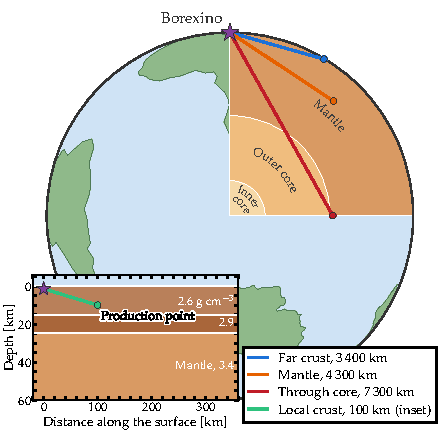
\includegraphics[width=\columnwidth]{geoneutrinos.pdf}
 \caption{\label{fig:geoneutrinos}The geometry of a geoneutrino measurement at Borexino, at Gran Sasso, 1.4~km underground. A quarter of the Earth is cut away to expose the PREM layers of \figu{prem}. Three chords reach production points beyond the local crust: in the far crust, 20~km deep and 3\,400~km away; in the mantle, 1\,000~km deep and 4\,300~km away; and at the base of the mantle, 2\,800~km deep and 7\,300~km away, on a path through the outer core. The inset shows the local crust, to scale in distance and stretched in depth, with the crust layers of PREM and a production point 10~km deep and 100~km away. See notebook \#28 for details.}
\end{figure}
%%%%%%%%%%%%%%%%%%%%%%%%%%%%%%%%%%%%%%%%%%%%%%%%%%%%%

Geoneutrinos are the $\bar{\nu}_e$ emitted in the decay chains of uranium-238 and thorium-232 inside the Earth\ \cite{Bellini:2013wsa}. Inverse beta decay detects them above 1.8~MeV; the uranium chain ends at 3.3~MeV, so that window holds the whole detectable spectrum. The sources are the crust and the mantle. Uranium and thorium are lithophile elements: they concentrate in silicate rock in the crust and the mantle; the metallic core contains neither. Potassium-40, the one radioactive nuclide sometimes assigned to the core, emits below the energy detection threshold. The core still enters the calculation, though, as the medium that neutrinos from the far side of the mantle cross. For a detector at or near the surface, the production points lie from a few km to a full Earth diameter away. As example, we take Borexino as the detector, located at Gran Sasso, 1.4~km underground.

Figure~\ref{fig:geoneutrinos} shows the setup. Four production points illustrate the four kinds of path a geoneutrino takes to Borexino. One lies in the local crust, 10~km deep and 100~km away, drawn in the inset. One lies in the far crust, 20~km deep and 3\,400~km away, on a path that dips into the upper mantle. One lies in the mantle, 1\,000~km deep and 4\,300~km away. The last lies at the base of the mantle, 2\,800~km deep and 7\,300~km away, on a path through the outer core.

%%%%%%%%%%%%%%%%%%%%%%%%%%%%%%%%%%%%%%%%%%%%%%%%%%%%%
\begin{figure}[t!]
 \centering
 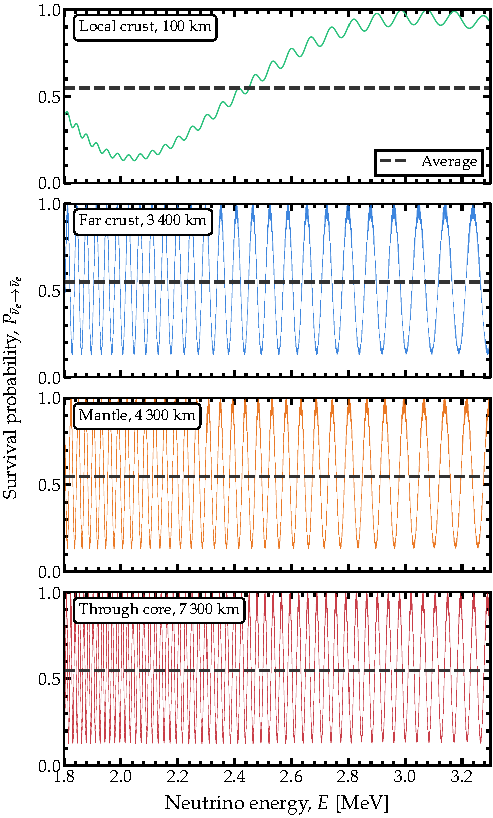
\includegraphics[width=\columnwidth]{geoneutrino_energy.pdf}
 \caption{\label{fig:geoneutrino_energy}Survival probability of geoneutrinos reaching Borexino, against energy, from the four production points of \figu{geoneutrinos}. Every curve resolves the pair split by $\Delta m^2_{31}$; it rides on the pair split by $\Delta m^2_{21}$ as a fine ripple. The average marked across every panel is the phase average in vacuum, 0.548; matter raises it along these chords by 0.3--0.8\%, less than the width of the line. Listing~\ref{lst:geoneutrinos} computes the four panels. See notebook \#28 for details.}
\end{figure}
%%%%%%%%%%%%%%%%%%%%%%%%%%%%%%%%%%%%%%%%%%%%%%%%%%%%%

Figure~\ref{fig:geoneutrino_energy} shows the survival probability against energy for these four production points. From the local crust, the pair split by $\Delta m^2_{21}$---the slow pair---completes three quarters of a cycle across the window; the pair split by $\Delta m^2_{31}$---the fast pair---rides on it, 26 cycles across the window. From the far crust, the mantle and the base of the mantle, the slow pair alone cycles 26 to 56 times across the window; the fast pair, 900 to 1\,900 times; the figure resolves both. A detector bins energy far more coarsely than that---which we do not show here---so a measurement of a distant reservoir sees instead the average probability.

In \figu{geoneutrino_energy}, the average value shown is the phase-average in vacuum, 0.548. Matter raises the average along these chords by 0.3--0.8\%, less than the width of the line, so the vacuum value serves our calculation. The size of that shift follows from Sec.~\ref{sec:averaged}. The passage through Earth is adiabatic: the largest jump in the electron density, at the core-mantle boundary, changes the mixing in matter by less than a percent at these energies, so the neutrino stays in the eigenstate it was produced in. The average is then \equ{averaged_varying} with $P^{\rm cross}$ the identity, fixed by the eigenbases at the two ends of the path alone. At both ends, the matter potential is a 1--2\% of the vacuum splitting of the slow pair, so each of those eigenbases is the nearly the vacuum one. The route of Sec.~\ref{sec:average_keyword} for a profile without declared discontinuities computes the average in matter. Along the mantle chord, with the density of PREM and the electron fraction of the mantle, next to the vacuum value, this is
\begin{pysnip}
from magnus.earth import (
 distance_traveled_inside_earth as chord,
 earth_radial_distance_from_depth as radius,
 density_matter_func_prem as prem,
 Y_E_MANTLE_PREM)

osc = gd.load_nufit_params('NuFIT 6.1')
c, depth = -0.552, 1000.0   # mantle chord
geo = dict(source_depth=depth,
           detector_depth=1.4)          # km
L = chord(c, **geo)                     # km
def rho(l):   # PREM along the chord, g/cm^3
    r = radius(c, l/gd.UNIT_KM, **geo)
    return prem(r,
                density_matter_ocean=2.65)
E = 2.5*gd.UNIT_MEV
P_m = oscprob.osc_prob_matter_std_potential(
 3, rho, E, L*gd.UNIT_KM, osc, average=True,
 nubar=True, nu_i=gd.NUE, nu_f=gd.NUE,
 electron_fraction=Y_E_MANTLE_PREM,
 density_matter_is_in_g_per_cm3=True)
# 0.551
P_v = oscprob.osc_prob_3nu_vacuum(E,
 L*gd.UNIT_KM, average=True, nubar=True,
 nu_i=gd.NUE, nu_f=gd.NUE)
# 0.548
\end{pysnip}

Listing~\ref{lst:geoneutrinos} computes the panels of \figu{geoneutrino_energy}. The Earth wrapper {\tt osc\_prob\_3nu\_earth} is called without {\tt average=True}: it returns the resolved probability of the panels. With {\tt average=True} it would instead take the energy-window route of Sec.~\ref{sec:average_keyword}, because it declares the PREM boundaries itself; the result would be a window mean with a standard error of 0.05. A production point enters through its depth and the cosine of its zenith angle at the detector, with {\tt nubar=True}. Every chord crosses PREM boundaries, six from the far crust, nine through the core; the call to {\tt osc\_prob\_3nu\_earth} declares them to the refinement ladder internally. The ocean layer of PREM is replaced by rock via {\tt density\_matter\_ocean}, since Gran Sasso is a continental site. The last call in Listing~\ref{lst:geoneutrinos} is the computation for the local crust. The production point sits at the end of its chord nearest to the detector, 100~km from it. The survival probability of a flavor is the same along a path and along its reverse, so the listing runs the segment from the detector to the production point, with the two depths in swapped roles and the zenith angle taken at the production point. 

%%%%%%%%%%%%%%%%%%%%%%%%%%%%%%%%%%%%%%%%%%%%%%%%%%%%%
\begin{lstlisting}[language=Python, caption={The four panels of \figu{geoneutrino_energy}: the survival probability of a geoneutrino reaching Borexino from the far crust, the mantle, the base of the mantle, and the local crust, across the detectable window, on one energy grid fine enough to resolve the pair split by $\Delta m^2_{31}$ on the longest chord. The call declares the PREM boundaries on each chord by itself. The ocean layer of PREM is replaced by rock. The local production point is run in reverse, from the detector.}, label={lst:geoneutrinos}, float=tbp]
import numpy as np
import magnus.oscprob as oscprob
import magnus.globaldefs as gd

# Twelve energies per cycle of the pair split by
# Dm31^2 on the longest chord, 7,300 km
E = 1/np.linspace(1/1.8, 1/3.3, 22500)*gd.UNIT_MEV

# Borexino, 1.4 km underground.  A production point
# enters as its depth and the cosine of its zenith
# angle at the detector; the call declares the PREM
# boundaries on the chord by itself.  The oscillation
# parameters are the defaults, NuFIT 6.1.
points = {'far crust': (20.0, -0.272),    # 3,400 km
          'mantle': (1000.0, -0.552),     # 4,300 km
          'core': (2800.0, -0.872)}       # 7,300 km
P = {}
for name, (depth, costhz) in points.items():
    P[name] = oscprob.osc_prob_3nu_earth(E,
     costhz=costhz, source_depth=depth*gd.UNIT_KM,
     detector_depth=1.4*gd.UNIT_KM, nubar=True,
     nu_i=gd.NUE, nu_f=gd.NUE,
     density_matter_ocean=2.65)

# The local point, 10 km deep and 100 km away, sits
# at the near end of its chord; the call runs every
# chord from the far end.  The survival probability
# is the same along a path and along its reverse, so
# run the segment from the detector, with the depths
# swapped and the zenith angle taken at the
# production point.
P['local'] = oscprob.osc_prob_3nu_earth(E,
 costhz=0.078, source_depth=1.4*gd.UNIT_KM,
 detector_depth=10.0*gd.UNIT_KM, nubar=True,
 nu_i=gd.NUE, nu_f=gd.NUE,
 density_matter_ocean=2.65)
\end{lstlisting}
%%%%%%%%%%%%%%%%%%%%%%%%%%%%%%%%%%%%%%%%%%%%%%%%%%%%%

%%%%%%%%%%%%%%%%%%%%%%%%%%%%%%%%%%%%%%%%%%%%%%%%%%%%%
\begin{figure}[t!]
 \centering
 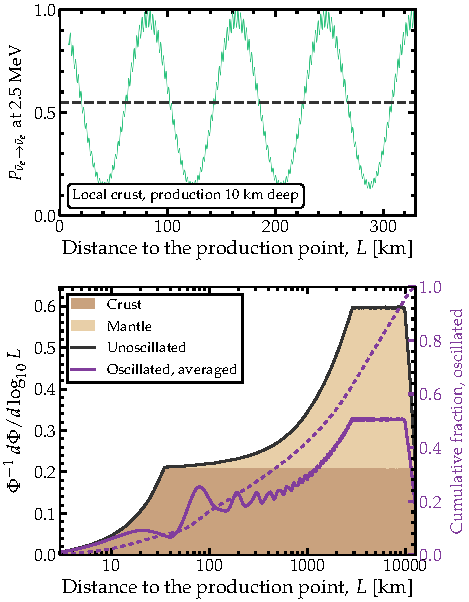
\includegraphics[width=\columnwidth]{geoneutrino_flux.pdf}
 \caption{\label{fig:geoneutrino_flux}Where the detectable geoneutrino flux at Borexino comes from and what oscillations leave of it. {\it Top}: the survival probability at 2.5~MeV against the distance to a production point 10~km deep, across the local crust, with the pair split by $\Delta m^2_{31}$ resolved; the horizontal line is the phase average. {\it Bottom}: the distribution of the flux of \equ{geoflux} in the distance to the production point, per unit $\log_{10} L$ and as a fraction of the total, for a spherically symmetric Earth with a 35-km crust holding 7~TW of radiogenic power, a mantle with the abundances of the geochemical model of Ref.~\cite{Bellini:2013wsa}, and no uranium or thorium in the core. The unoscillated curve has $\langle P_{\bar\nu_e \to \bar\nu_e} \rangle = 1$; the shading splits it between the two reservoirs. The oscillated curve folds in the survival probability averaged over the detectable window with equal weight in energy; its cumulative fraction is on the right axis. See notebook \#28 for details.}
\end{figure}
%%%%%%%%%%%%%%%%%%%%%%%%%%%%%%%%%%%%%%%%%%%%%%%%%%%%%

Figure~\ref{fig:geoneutrino_flux} shows how the detectable flux is distributed over the distance to the production point and how much of it survives the oscillations. A flux measurement weighs the curves of \figu{geoneutrino_energy} by that distribution. The Earth model chosen for the figure is the simplest one that carries both reservoirs: a spherically symmetric crust 35-km thick holding 7~TW of radiogenic power at a thorium-to-uranium ratio of 4.5, a mantle with the abundances of the geochemical model of Ref.~\cite{Bellini:2013wsa}, no uranium or thorium in the core, and the density of PREM throughout. The flux at the detector is
\begin{equation}
 F = \int_\oplus d^3r \, \frac{\varepsilon(\mathbf{r})}{4 \pi L^2} \, \langle P_{\bar\nu_e \to \bar\nu_e} \rangle (L) \,, \qquad L = \lvert \mathbf{r} - \mathbf{r}_{\rm det} \rvert \,,
 \label{equ:geoflux}
\end{equation}
where $\varepsilon(\mathbf{r})$ is the number of detectable $\bar{\nu}_e$ emitted per unit volume and time at position $\mathbf{r}$, fixed by the density of PREM and the abundances above. The survival probability from that point, $\langle P_{\bar\nu_e \to \bar\nu_e}(L) \rangle$, is the mean over the detectable window, 1.8--3.3~MeV. In spherical coordinates centered on the detector, $d^3r = L^2 \, dL \, d\Omega$ and the $L^2$ cancels: the production points between $L$ and $L + dL$ contribute $dL / 4\pi$ times the emissivity integrated over the directions in which that shell lies inside the Earth. The lower panel of \figu{geoneutrino_flux} shows this distribution per unit $\log_{10} L$, normalized to the total flux without oscillations, so that the area under a curve between two distances is the share of the flux from between them. In the unoscillated curve (normalized so $\langle P_{\bar\nu_e \to \bar\nu_e} \rangle = 1$), 61\% of the detectable flux comes from the crust, 17\% from within 100~km, 30\% from within 350~km, and 43\% from within 1\,000~km.

The oscillated curve is the same distribution multiplied by $\langle P_{\bar\nu_e \to \bar\nu_e}(L) \rangle$, computed in two pieces. Up to 331~km, the probability is propagated through the crust with the last call of Listing~\ref{lst:geoneutrinos}, once per distance on the grid, then averaged over the energy window. Beyond 331~km, the vacuum probability averaged over the same window is used instead: matter changes the average by 0.01 at that distance and by less farther out (\figu{geoneutrino_energy}). The upper panel shows the probability through the crust at 2.5~MeV, before the average: the slow pair oscillates every 84~km at  and the fast pair every 2.5~km, as a ripple. In the lower panel, the oscillated curve still ripples out to a few hundred km, where the window holds too few cycles of the slow pair to average them out; farther out it is smooth. Over the whole Earth, oscillations leave 54\% of the detectable flux.

%%%%%%%%%%%%%%%%%%%%%%%%%%%%%%%%%%%%%%%%%%%%%%%%%%%%%

\subsubsection{Neutrino tomography of the Sun}
\label{sec:solar_tomography}

%%%%%%%%%%%%%%%%%%%%%%%%%%%%%%%%%%%%%%%%%%%%%%%%%%%%%
\begin{figure}[t!]
 \centering
 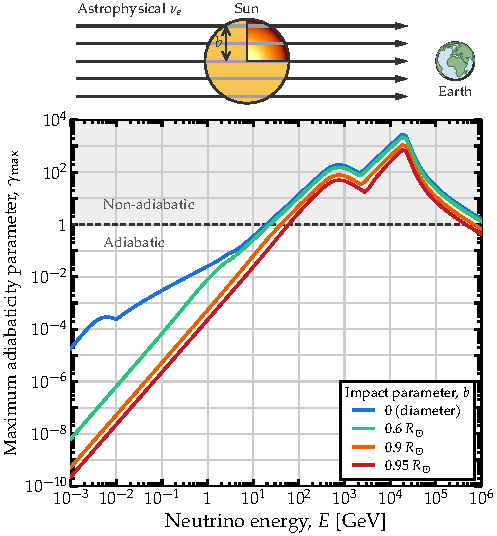
\includegraphics[width=\columnwidth]{solar_adiabaticity.pdf}
 \caption{\label{fig:solar_adiabaticity}{\it Top}: the setup. An isotropic flux of $\nu_e$ crosses the Sun and continues to Earth, where it may oscillate. The impact parameter $b$ is marked on one ray. {\it Bottom:} Adiabaticity of a neutrino trajectory through the Sun against neutrino energy, computed with \magnus\ on the B16-GS98 solar density profile\ \cite{Vinyoles:2016djt}, tabulated up to the surface, for four impact parameters, each defining a chord through the Sun. The parameter $\gamma_{\rm max}$ is the adiabaticity parameter of \equ{hf}, evaluated at its maximum value along the chord and over the three pairs of eigenvalue levels. See notebook \#28 and Sec.~\ref{sec:solar_tomography} for details.}
\end{figure}
%%%%%%%%%%%%%%%%%%%%%%%%%%%%%%%%%%%%%%%%%%%%%%%%%%%%%

Neutrinos made outside the Solar System cross the Sun on their way to Earth. At around 10~MeV, they are mainly from the diffuse supernova neutrino background. From TeV to PeV, they are part of the high-energy astrophysical flux. Both fluxes are isotropic, so a share of each passes through the Sun before reaching a detector. Below, we compute what that does to their oscillations, using the B16-GS98 profile\ \cite{Vinyoles:2016djt} of Table~\ref{tab:solar_models}. Unlike BS2005-AGS,OP, it is tabulated up to the solar surface, so every chord crosses the whole Sun.

A neutrino from such a source has traveled far enough that the wave packets of its mass eigenstates have separated. What arrives is an incoherent mixture, so what is measured is the phase-averaged probability of Sec.~\ref{sec:averaged} instead of the instantaneous one. Inside the Sun, the Hamiltonian changes along the path, so the phase average is carried along it (Sec.~\ref{sec:averaged}). The neutrino starts decohered in the eigenbasis at the point of entry and follows the instantaneous eigenstates. It crosses each non-adiabatic region through a Magnus patch and is read out in flavor at exit. Where no crossing is non-adiabatic, the result is \equ{averaged_varying}, with the level-crossing matrix $P^{\rm cross}$ between the eigenbases at entry and exit.

Both ends of the path lie in vacuum, where the eigenvectors are the vacuum mixing matrix, so $\mathbb{V}(l_0) = \mathbb{V}(l_1) = \mathbb{U}$ in \equ{averaged_varying}. An adiabatic passage would make $P^{\rm cross}$ the identity. Equation (\ref{equ:averaged_varying}) would then collapse to \equ{averaged} evaluated in vacuum, leaving no trace of the Sun. Whether or not the passage is adiabatic depends on the energy, via \equ{hf}.

A solar neutrino behaves differently: because it is born deep inside the Sun, at high density, it begins as a matter eigenstate. The adiabatic passage outward then maps it onto a single mass eigenstate. That is the MSW effect of Sec.~\ref{sec:sun}. A neutrino crossing from outside meets the same density profile, but enters it as a vacuum mass eigenstate. Because the density vanishes at both ends of that path, adiabatic passage keeps the neutrino in one eigenstate of the instantaneous $\mathbb{H}$ and returns it to the mass eigenstate it entered with. What separates the two cases is where each path begins and ends.

Figure~\ref{fig:solar_adiabaticity} shows how adiabatic the passage is, from MeV to PeV, for four choices of the impact parameter at which the neutrinos hit the Sun, and assuming three flavors. Equation~(\ref{equ:hf}) attaches an adiabaticity parameter $\gamma_{jk}(l)$ to every pair of eigenvalues (1-2, 1-3, 2-3) of $\mathbb{H}$ at every point $l$ of the trajectory. It is large where two of those eigenvalues approach each other and small where they stay apart. The figure plots $\gamma_{\rm max}$, the largest value found anywhere along the chord and over all three pairs, so a curve above one means the neutrino moves between eigenstates of $\mathbb{H}$ somewhere on its way through. The parameter can be computed using the {\tt adiabatic} module of \magnus:
\begin{pysnip}
import numpy as np
import magnus.adiabatic as adiabatic
import magnus.hamiltonians as ham
import magnus.matter as matter
import magnus.globaldefs as gd
import magnus.solarmodels as solarmodels

R = gd.SUN_RADIUS*gd.UNIT_KM
ne_sun = solarmodels.electron_density_profile(
    'B16-GS98')
b = 0.3*R                # impact parameter
half = np.sqrt(R**2 - b**2)
E = 100.0*gd.UNIT_GEV
hv = ham.hamiltonian_3nu_vacuum(E, **osc)

def ne(l):
    """Electron density on the chord."""
    r = np.sqrt((l - half)**2 + b**2)
    return ne_sun(r)

def H(l):
    """Hamiltonian at l along the chord."""
    h = np.array(hv, dtype=complex)
    h[0, 0] += matter.VCC_func(l, ne)
    return h

info = {}
adiabatic.find_nonadiabatic_windows(
    H, 0.0, 2*half, n_probe=20000,
    info=info)
info['gamma_max']        # 13.7460
\end{pysnip}
Here, {\tt ne\_sun} is the B16-GS98 table, interpolated in its logarithm, {\tt ne} evaluates it along the chord, and {\tt hv} is the vacuum Hamiltonian at this energy. The value shown is for a $100$-GeV neutrino crossing at an impact parameter of $b = 0.3\,R_\odot$.

The parameter $\gamma_{\rm max}$ grows with energy because the vacuum splitting $\Delta m^2/2E$ shrinks while the matter potential in the Sun stays fixed. It is attained just inside the 1-2 resonance, where the matter potential equals $\Delta m^2_{21}\cos 2\theta_{12}/2E$, independently of the impact parameter. As the energy grows, that density is reached further out: $\gamma_{\rm max}$ sits at $0.97\,R_\odot$ at $100$~GeV, at $0.990\,R_\odot$ at 1~TeV, and at $0.998\,R_\odot$ at 100~TeV. By 1~PeV, it reaches $5\times10^6$ on the diameter. [Figure~\ref{fig:solar_adiabaticity} shows only the effect of oscillations; absorption, which matters above the GeV scale, is outside what \magnus\ models (Sec.~\ref{sec:limitations}).]

%%%%%%%%%%%%%%%%%%%%%%%%%%%%%%%%%%%%%%%%%%%%%%%%%%%%%
\begin{figure*}[t!]
 \centering
 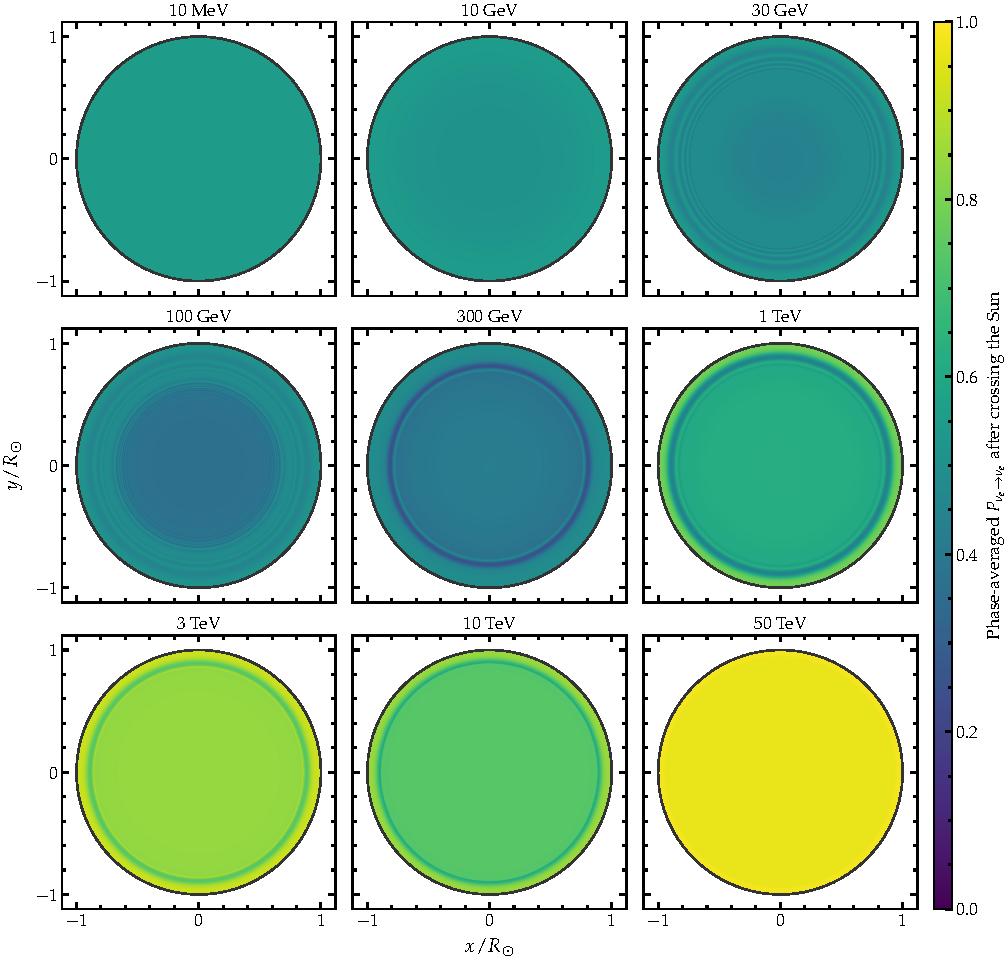
\includegraphics[width=\textwidth]{solar_tomography.pdf}
 \caption{\label{fig:solar_tomography}The Sun seen face-on in the $\nu_e$ survival channel, computed with \magnus\ on the B16-GS98 solar density profile\ \cite{Vinyoles:2016djt}. The line of sight runs into the page, so each point of the disk is an impact parameter and the neutrino crosses the whole Sun along it. The color is the phase-averaged $P_{\nu_e \to \nu_e}$ at exit, for a relative energy spread of $10\%$, averaged over the area of each pixel. See notebook \#28 and Sec.~\ref{sec:solar_tomography} for details.}
\end{figure*}
%%%%%%%%%%%%%%%%%%%%%%%%%%%%%%%%%%%%%%%%%%%%%%%%%%%%%

Figure~\ref{fig:solar_tomography} shows the averaged survival probability across the face of the Sun, at selected energies. The line of sight runs into the page, so each point in the disk fixes the impact parameter of one trajectory, along which the neutrino crosses the whole Sun. For one impact parameter, the probability is computed via
\begin{pysnip}
import magnus.oscprob as oscprob

# The chord above: b = 0.3 R_sun
P = oscprob.osc_prob_matter_std_potential(
    3, ne, E, 2*half, average=True,
    osc_params=osc, L0=0.0, nu_i=gd.NUE,
    nu_f=gd.NUE,
    density_is_of_number_of_electrons=True)
P                        # 0.304987
\end{pysnip}
Here, {\tt average=True} returns the phase average along the chord, without sampling energies. Section~\ref{sec:averaging_is_not_estimating} shows why averaging a scan of probabilities does not necessarily reproduce this.  (The phase average keeps the matter phase $\int V_{\rm CC}\,dl$, $8676$~rad across the diameter. That phase does not depend on the energy, so no energy spread averages it. It draws rings in the core of the disk, $1.8\times10^{-4}\,R_\odot$ apart at $b = 0.11\,R_\odot$ and $5.1\times10^{-4}\,R_\odot$ apart at $b = 0.3\,R_\odot$. At 1~TeV, they move $P$ by up to about $\pm 0.03$. The value printed above sits on one of them: within one ring spacing of $b = 0.3\,R_\odot$, $P$ ranges from 0.282 to 0.308. Each pixel of \figu{solar_tomography} is therefore averaged over its area. The panels from 30~GeV to 3~TeV sample $7\,773$ impact parameters each, $6\,772$ of them inside $b = 0.5\,R_\odot$.)

At $10$~MeV, the disk is uniform at about $\sum_i |\mathbb{U}_{ei}|^4 \approx 0.55$: the Sun is transparent, exactly as $P^{\rm cross} = \mathbb{1}$ requires. At intermediate energies, rings appear, within the non-adiabatic region of \figu{solar_adiabaticity}. They are drawn by the crossings: where the passage is not adiabatic, the level-crossing probabilities depart from the identity. The phase average also keeps part of the interference that \equ{averaged_varying} discards. That interference changes the depth of the rings: at 300~GeV, the deepest one reaches $P = 0.03$ at $b = 0.81\,R_\odot$, against $0.20$ in \equ{averaged_varying}. From 300~GeV up, the deepest ring moves outward, to $b = 0.89\,R_\odot$ at 1~TeV and $0.91\,R_\odot$ at 10 and 50~TeV. At 50~TeV, the disk is uniform again, but for a different reason than at 10~MeV: a $\nu_e$ that enters the Sun leaves it as a $\nu_e$, at every impact parameter. The Sun only adds a phase to it; the survival probability does not depend on that phase.

To be clear, no neutrino telescope resolves any of this structure. While the Sun has been imaged in MeV neutrinos, most famously by Super-Kamiokande, the width of that image is set by the angular resolution of the detector: the recoil electron of neutrino-electron elastic scattering carries the neutrino direction only to within tens of degrees, against a disk of half a degree. At tens of TeV, the angular resolution is better, but still comparable to the size of the disk itself. The rings of \figu{solar_tomography} are a few arcseconds to a few arcminutes wide. The rings of the matter phase, over which each pixel is averaged, are $0.2$ to $4$ arcseconds apart. In addition, the panels of \figu{solar_tomography} at GeV energies---where the rings first appear---lie in a band where no astrophysical neutrino flux has been identified above the atmospheric background.

%%%%%%%%%%%%%%%%%%%%%%%%%%%%%%%%%%%%%%%%%%%%%%%%%%%%%

\subsubsection{Astrophysical relativistic jet}
\label{sec:jet}

Gamma-ray bursts are the relativistic jets that some massive stars launch as they collapse. Shells of plasma ejected by the central engine collide with one another along the jet; protons accelerated at those collisions make neutrinos of TeV to PeV energies\ \cite{Bustamante:2014oka}. The jet itself does change their flavor composition: at the radii where the collisions happen, $10^{13}$--$10^{15}$~cm, its density is around $10^{-11}$~g~cm$^{-3}$, nine orders of magnitude below the density at which a TeV neutrino resonates; the phase that the jet matter adds to the evolution is only $10^{-4}$. Matter effects arise only while the jet is still inside the star, in the choked jets that never break out and in the precursor phase of the jets that do\ \cite{Mena:2006eq, Razzaque:2009kq, Sahu:2010ap, Varela:2014mma, Xiao:2015gea}. The neutrinos then cross the stellar envelope. Its density falls from about 1~g~cm$^{-3}$ at the head of the jet to zero at the surface; somewhere along, neutrinos between $100$~GeV and $100$~TeV meet their 1-3 resonance. At the low energy end, the crossing is adiabatic and the neutrino leaves the star in a mass eigenstate; at the high end, it is not: the flavor content then survives. Therefore, the flavor ratios at Earth depend on the neutrino energy, in a way that reflects the density profile of the star\ \cite{Razzaque:2009kq, Xiao:2015gea}.

As example, we take a jet at $r_0 = 6.3 \cdot 10^{10}$~cm inside a blue supergiant of radius $R_\star = 3 \cdot 10^{12}$~cm, with the hydrogen envelope of \Refs\ \cite{Mena:2006eq, Razzaque:2009kq}, $\rho(r) = 3.3 \cdot 10^{-6}\,(R_\star/r - 1)^3$~g~cm$^{-3}$, and an electron fraction of $Y_e = 1$:
\begin{pysnip}
import numpy as np
import magnus.globaldefs as gd
import magnus.hamiltonians as ham
import magnus.oscprob as oscprob

OSC = gd.load_nufit_params('NuFIT 6.1')
CM = 1.0e-5*gd.UNIT_KM   # One cm in eV^-1
RSTAR = 3.0e12           # Star's radius, cm
R0 = 6.3e10              # Jet head, cm

def rho(l):
    """Density, g/cm3, at l in eV^-1."""
    return 3.3e-6*(RSTAR/(l/CM) - 1.0)**3
\end{pysnip}
The density at the head is $0.33$~g~cm$^{-3}$. The oscillation length there is set by the potential, $2\pi/V_{\rm CC} = 5 \cdot 10^{9}$~cm, a tenth of $r_0$, so the phase accumulated across the whole envelope is modest. The observable, the phase-averaged probability of \equ{averaged_varying}, is built here from the evolution operator rather than from probabilities. The scenario functions return the operator alongside the probabilities when asked ({\tt return\_evolution\_operator=True}), with the refinement ladder choosing the slabs internally:
\begin{pysnip}
E = 1.0*gd.UNIT_TEV
out = oscprob.osc_prob_matter_std_potential(
    3, rho, E, RSTAR*CM, OSC, L0=R0*CM,
    electron_fraction=1.0,
    rtol=1.0e-6, atol=1.0e-6,
    density_matter_is_in_g_per_cm3=True,
    return_evolution_operator=True)
P, U = out
\end{pysnip}
Here, {\tt P} is the probability matrix at the surface of the star and {\tt U} is the evolution operator from the jet head to the surface, in the flavor basis.

%%%%%%%%%%%%%%%%%%%%%%%%%%%%%%%%%%%%%%%%%%%%%%%%%%%%%
\begin{figure}[t!]
 \centering
 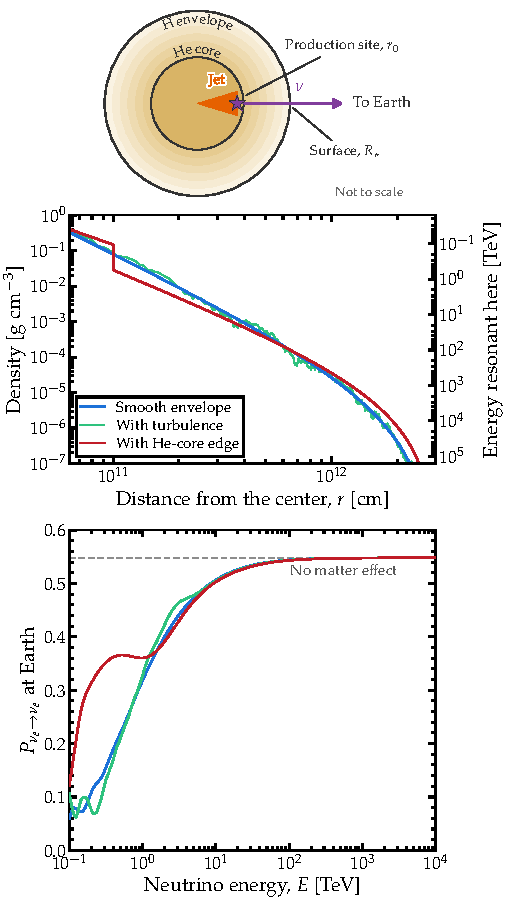
\includegraphics[width=\columnwidth]{jet.pdf}
 \caption{\label{fig:jet}Neutrinos from a relativistic jet inside a collapsing star. \textit{Top:} the setup. Neutrinos are made at the head of the jet, at $r_0 = 6.3 \cdot 10^{10}$~cm from the center, and leave the star at $R_\star = 3 \cdot 10^{12}$~cm. \textit{Middle:} matter density along their path, for a smooth envelope, the same envelope with turbulence overlaid, and the same envelope with a drop in density at the edge of the helium core. The right axis gives the energy whose 1-3 resonance lies at each density. \textit{Bottom:} probability that a $\nu_e$ produced at the jet head is detected as $\nu_e$ at Earth, against its energy, for the three envelopes. See notebook \#28 and Sec.~\ref{sec:jet} for details.}
\end{figure}
%%%%%%%%%%%%%%%%%%%%%%%%%%%%%%%%%%%%%%%%%%%%%%%%%%%%%

What a telescope detects is not the flavor content at the surface of the star: the neutrino travels a cosmological distance afterwards, over which the phases between its mass components average out, so it arrives as an incoherent mixture of mass eigenstates\ \cite{Razzaque:2009kq}. Its probability is the phase-averaged form of \equ{averaged_varying}, with the eigenbasis at detection being the mixing matrix in vacuum, $\mathbb{R}$. The factor in it that carries the star, the probability that a neutrino produced as $\nu_\alpha$ leaves it as the mass eigenstate $\nu_i$, is read off the evolution operator as $\lvert [\mathbb{R}^\dagger \mathbb{U}]_{i\alpha} \rvert^2$:
\begin{pysnip}
# Vacuum mass states; the content of each in
# the state that leaves the star, by flavor
hv = np.array(ham.hamiltonian_3nu_vacuum(
    E, **OSC), dtype=complex)
w, R = np.linalg.eigh(hv)
content = abs(R.conj().T @ U)**2

# Phases average on the way to Earth
P_earth = abs(R)**2 @ content
P_earth[gd.NUE, gd.NUE]    # 0.315
\end{pysnip}
Thus, the probability computed is $P_{\nu_\alpha \to \nu_\beta} = \sum_i \left\lvert \left[ \mathbb{R}^\dagger\, \mathbb{U} \right]_{i\alpha} \right\rvert^2 \left\lvert \mathbb{R}_{\beta i} \right\rvert^2$.  Without matter effects the same construction gives $0.55$.

Figure~\ref{fig:jet} shows this probability between 0.1~TeV and 10~PeV for three density envelopes. The neutrinos are not all made at the same point: the production region at the jet head is about one oscillation length across, so each curve averages over production points spread over that length. Without this average, the lowest energies would show an interference pattern, since their resonance lies only a few oscillation lengths from the head; a region of that size washes it out. The first envelope is the smooth profile above. The second overlays turbulence on it: a single realization of forty modes with a Kolmogorov spectrum, with wavelengths from $10^{10}$ to $10^{12}$~cm at a root-mean-square amplitude of twenty percent. The third is model C of \Refs\ \cite{Mena:2006eq}, the same star with the density dropping by a factor of five at the edge of the helium core, $r = 10^{11}$~cm; in the code, that edge is declared to the ladder as a breakpoint. Listing~\ref{lst:jet} is the calculation behind the figure.

%%%%%%%%%%%%%%%%%%%%%%%%%%%%%%%%%%%%%%%%%%%%%%%%%%%%%
\begin{lstlisting}[language=Python, caption={Computing the data in \figu{jet} with \magnus: the phase-averaged $\nu_e$ survival probability at Earth for neutrinos from a jet head at $r_0$, through the three envelopes. Each call returns the evolution operator from the refinement ladder alongside the probabilities; the projection onto the vacuum mass states and the sum over them are \equ{averaged_varying}, with the eigenbasis at detection the vacuum one. The eight production points span one oscillation length at the jet head, $4.9 \cdot 10^{9}$~cm. The turbulent envelope is one realization of forty Kolmogorov modes between $10^{10}$ and $10^{12}$~cm at twenty percent rms; the stepped one is model C of \Refs\ \cite{Mena:2006eq}, with the drop at the helium-core edge declared through {\tt t\_breakpoints}. See notebook \#28 and Sec.~\ref{sec:jet} for details.}, label={lst:jet}, float=t]
import numpy as np
import magnus.globaldefs as gd
import magnus.hamiltonians as ham
import magnus.oscprob as oscprob

OSC = gd.load_nufit_params('NuFIT 6.1')
CM = 1.0e-5*gd.UNIT_KM               # One cm in eV^-1
RSTAR, R0, RHE = 3.0e12, 6.3e10, 1.0e11      # cm
E = np.geomspace(0.1, 1.0e4, 161)*gd.UNIT_TEV

# The three envelopes, g/cm3, r in cm
def smooth(r):
    return 3.3e-6*(RSTAR/r - 1.0)**3

rng = np.random.default_rng(7)        
lam = np.geomspace(1.0e12, 1.0e10, 40)  # Modes, cm
k = 2*np.pi/lam
amp = k**(-1/3)                         # Kolmogorov
amp *= 0.20/np.sqrt(0.5*np.sum(amp**2)) # 20% rms
phi = rng.uniform(0.0, 2*np.pi, 40)
def turbulent(r):
    d = np.sum(amp*np.cos(k*r + phi))
    return smooth(r)*(1.0 + d)

def stepped(r):            # Mena et al., model C
    x = RSTAR/r - 1.0
    return 6.3e-6*(20.0*x**2.1 if r < RHE else x**2.5)

# Production points spread over one oscillation
# length at the jet head
r0s = R0 + 4.9e9*np.arange(8)/8.0

def p_earth(rho, **extra):
    """P at Earth, Eq. (26), averaged over the
    production points."""
    P_out = np.zeros((len(E), 3, 3))
    for r0 in r0s:
        P, U = oscprob.osc_prob_matter_std_potential(
            3, lambda l: rho(l/CM), E, RSTAR*CM, OSC,
            L0=r0*CM, electron_fraction=1.0,
            density_matter_is_in_g_per_cm3=True,
            rtol=1.0e-6, atol=1.0e-6,
            return_evolution_operator=True, **extra)
        for i, e in enumerate(E):
            hv = np.array(ham.hamiltonian_3nu_vacuum(
                e, **OSC), dtype=complex)
            w, R = np.linalg.eigh(hv)
            content = abs(R.conj().T @ U[i])**2
            P_out[i] += abs(R)**2 @ content/len(r0s)
    return P_out

P_smooth = p_earth(smooth)
P_turb = p_earth(turbulent)
P_step = p_earth(stepped, t_breakpoints=[RHE*CM])
# Drawn: P_smooth[:, gd.NUE, gd.NUE], and the others
\end{lstlisting}
%%%%%%%%%%%%%%%%%%%%%%%%%%%%%%%%%%%%%%%%%%%%%%%%%%%%%

The smooth envelope sets the trend. At 0.1~TeV, a $\nu_e$ leaves the star mostly as $\nu_3$---which has the least electron content among the three mass eigenstates---and so is rarely detected as $\nu_e$. With rising energy, the survival probability climbs to its vacuum value, reached at 100~TeV. The reason is where the resonance sits. A neutrino of higher energy resonates farther out, where the density falls more gently, but its oscillation length grows faster than that gain, so the crossing becomes abrupt and the flavor content survives it. The PeV neutrinos that IceCube detects come out of the star as if it were not there.

Turbulence shifts the smooth curve by up to 0.05 below a few TeV. Those are the energies whose resonance lies where the modes of the realization match the local oscillation length; the mechanism is that of Sec.~\ref{sec:turbulence}. The drop at the helium-core edge has a larger effect. The energies whose resonance density lies inside the drop, 0.15--0.7~TeV, do not cross the resonance gradually: they meet it in one jump, at the edge, so the crossing is non-adiabatic regardless of the energy and the flavor content survives. The result is the low-energy plateau in the probability seen in \figu{jet}. Above the band, the two envelopes agree again.

Each envelope costs a few minutes for the energies drawn and the eight production points averaged. The ladder settles on a few thousand slabs per energy at the tolerance requested ($10^{-6}$), with the helium-core edge declared to it as a breakpoint.

%%%%%%%%%%%%%%%%%%%%%%%%%%%%%%%%%%%%%%%%%%%%%%%%%%%%%

\subsubsection{Long-range interactions in the Sun}
\label{sec:lri_sun}

%%%%%%%%%%%%%%%%%%%%%%%%%%%%%%%%%%%%%%%%%%%%%%%%%%%%%
\begin{figure}[t!]
 \centering
 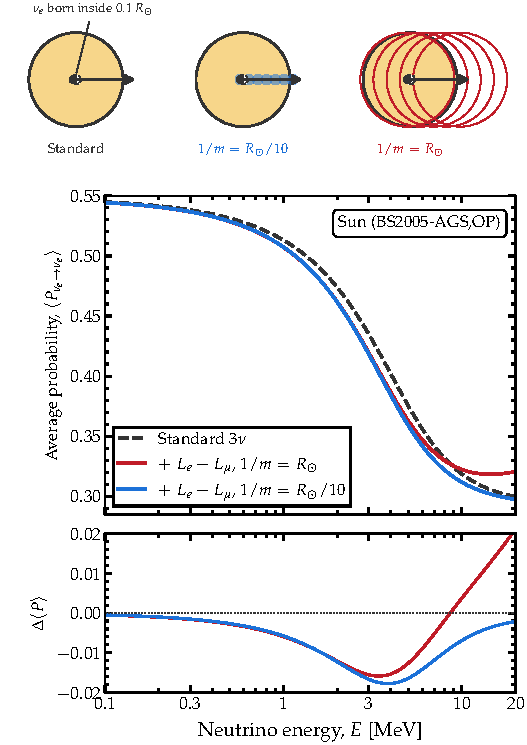
\includegraphics[width=\columnwidth]{solar_long_range.pdf}
 \caption{\label{fig:solar_lri}Phase-averaged survival probability of a solar neutrino under a long-range $L_e - L_\mu$ interaction sourced by the electrons of the Sun. \textit{Top:} what each mediator range lets the neutrino feel. A $\nu_e$ born inside $0.1\,R_\odot$ leaves along the ray drawn; the discs are the electrons within $1/m$ of it as it goes. The charged-current potential is local and carries no disc; at $1/m = R_\odot/10$ the neutrino feels a narrow tube; at $1/m = R_\odot$ it feels most of the Sun at once, and past the surface. \textit{Middle:} $\langle P_{\nu_e \to \nu_e}\rangle$ along a radial ray of the BS2005-AGS,OP model of \figu{solar}, without the new potential and with it at the two ranges. The coupling is fixed separately for each range so that $V_{e\mu}$ is a tenth of $V_{\rm CC}$ at the center; the two curves then differ only through the shape of the potential along the ray. \textit{Bottom:} the difference from the standard case. See notebooks \#19 and \#28 and Sec.~\ref{sec:lri_sun} for details.}
\end{figure}
%%%%%%%%%%%%%%%%%%%%%%%%%%%%%%%%%%%%%%%%%%%%%%%%%%%%%

This example adds to the Hamiltonian a term that \magnus\ does not ship, written as Sec.~\ref{sec:building_new_hamiltonian} describes, then carries it through the same averaging machinery as the standard solar case of Sec.~\ref{sec:sun}. The term comes from gauging $L_e - L_\mu$, the difference of the electron and muon lepton numbers, an anomaly-free combination that admits a new light gauge boson $Z'$ that acts as a new mediator\ \cite{He:1990pn, Foot:1994vd}. The charge $Q \equiv L_e - L_\mu$ is $+1$ for the electron and $\nu_e$, $-1$ for the muon and $\nu_\mu$, zero for every other field of the Standard Model, so the electrons of a body source a potential that the three neutrino flavors feel differently, via the Hamiltonian
\begin{equation}
 \label{equ:h3_lri}
 \mathbb{H}^{\rm LRI}(E, l)
 =
 \frac{\mathbb{A}}{E} + V_{\rm CC}(l)\,\mathbb{P}
 + V_{e\mu}(l)\,{\rm diag}\left(1, -1, 0\right) \;,
\end{equation}
where the first two terms are the vacuum and charged-current matter terms of Sec.~\ref{sec:recap}; the third is the modification.

The new potential is non-local. An electron sources a Yukawa potential centered on its own position, so a neutrino at $\mathbf{r}$ feels an integral over the electrons around it,
\begin{equation}
 \label{equ:yukawa}
 V_{e\mu}(\mathbf{r})
 =
 \frac{g^{\prime 2}}{4\pi}
 \int d^3r^\prime \, n_e(\mathbf{r}^\prime) \,
 \frac{e^{-m \lvert \mathbf{r} - \mathbf{r}^\prime \rvert}}
      {\lvert \mathbf{r} - \mathbf{r}^\prime \rvert} \;,
\end{equation}
with $g^\prime$ the new gauge coupling and $m$ the mediator mass. Where $V_{\rm CC}$ reads the density at the neutrino's own position, \equ{yukawa} reaches every electron within about $1/m$ of it. At mediator masses light enough for that range to span the body, the potential depends on how many electrons the body holds and only weakly on where they sit\ \cite{Wise:2018rnb}. For a spherical body, like the Sun, the angular integral is elementary; \equ{yukawa} then splits into an interior and an exterior piece,
\begin{equation}
 \label{equ:yukawa_1d}
 \begin{split}
 V_{e\mu}(r)
 = {} &
 \frac{g^{\prime 2}}{r}\, e^{-m r}
 \int_0^{r} dr^\prime\, r^{\prime 2}\, n_e(r^\prime)\, {\rm shc}(m r^\prime) \\
 & + g^{\prime 2}\, {\rm shc}(m r)
 \int_r^{R_\odot} dr^\prime\, r^\prime\, n_e(r^\prime)\, e^{-m r^\prime} \;,
 \end{split}
\end{equation}
with ${\rm shc}(x) \equiv \sinh(x)/x$ and $m \equiv m_{Z'}$. Both integrals run over the density profile, so one pass over the table of densities of a solar model serves every position along the ray. The form also holds for a massless mediator: as $m \to 0$, both ${\rm shc}$ and the exponential tend to 1, leaving the Coulomb-like potential of the electrons enclosed within $r$ and of those outside it. Notebook \#19 derives \equ{yukawa_1d} and checks its evaluation against the closed form that a uniform ball has at any mediator mass.

Listing~\ref{lst:arbitrary} is the calculation behind \figu{solar_lri}. The electron density is the BS2005-AGS,OP table of \figu{solar}. The potential is \equ{yukawa_1d} on that table at two mediator ranges, $1/m = R_\odot$ and $R_\odot/10$, \ie, $m  = 2.8 \cdot 10^{-16}$ and $2.8 \cdot 10^{-15}$~eV, respectively. The coupling is fixed separately for each so that $V_{e\mu}$ is a tenth of $V_{\rm CC}$ at the center. What then differs between the two is only the shape of the potential along the ray. The Sun makes that difference large: its electron density falls by five orders of magnitude from the center to the surface, so $V_{\rm CC}$ falls with it, while $V_{e\mu}$, an integral over the whole body, does not. With the objects of the listing, at half a solar radius,
\begin{pysnip}
half = np.searchsorted(r, 0.5*R_SUN)
v_emu[1.0][half]/vcc[half]     # 2.49
v_emu[0.1][half]/vcc[half]     # 0.38
\end{pysnip}
The longer-ranged potential is about $2.5\,V_{\rm CC}$ and the shorter-ranged one, $0.4\,V_{\rm CC}$. Both started at $0.1\,V_{\rm CC}$ at the center, so both have fallen less steeply than $V_{\rm CC}$ itself. At the surface, where $V_{\rm CC}$ has all but vanished, the shorter-ranged potential is $6\,V_{\rm CC}$ and the longer-ranged one, $10^3\,V_{\rm CC}$. The sketch atop \figu{solar_lri} shows why: at $1/m = R_\odot$ the neutrino feels most of the Sun at once, wherever it is.

The Hamiltonian is one function returning the sum of the three terms, written to take an array of positions so that the engine evaluates it once per slab rather than once per quadrature node (Sec.~\ref{sec:cost}). The averaged probability comes from the same call that serves the standard case, since nothing in it asks what the Hamiltonian contains. At $10$~MeV,
\begin{pysnip}
i = np.argmin(abs(Es - 10.0*gd.UNIT_MEV))
P_std[i]                      # 0.318
P_lri[1.0][i], P_lri[0.1][i]  # 0.322, 0.311
\end{pysnip}

%%%%%%%%%%%%%%%%%%%%%%%%%%%%%%%%%%%%%%%%%%%%%%%%%%%%%
\begin{lstlisting}[language=Python, caption={Computing the data in \figu{solar_lri} with \magnus: the $L_e - L_\mu$ interaction of \equ{h3_lri} in the Sun. The electron density is read from the BS2005-AGS,OP table\ \cite{Bahcall:2004pz}; $V_{e\mu}$ is \equ{yukawa_1d} on that table, with the coupling fixed so that it is a tenth of $V_{\rm CC}$ at the center. The vacuum and matter terms come from the shipped builders; the new term is the one line written here. The averaged probability of \equ{averaged_varying} is the same {\tt average=True} the wrappers take, on the direct route. Notebooks \#19 and \#28 derive the potential and draw the figure.}, label={lst:arbitrary}, float=tbp]
import numpy as np
import magnus.globaldefs as gd
import magnus.hamiltonians as hamiltonians
import magnus.matter as matter
import magnus.oscprob as oscprob

osc = gd.load_nufit_params('NuFIT 6.1')

# The BS2005-AGS,OP model: radius, density in g/cm3
# and hydrogen mass fraction are columns 1, 3 and 6
rows = [l.split() for l in open('bs05_agsop.dat')]
tab = np.array([[float(x) for x in f] for f in rows
                if len(f) == 12 and f[0][0].isdigit()])
r = tab[:, 1]*gd.SUN_RADIUS*gd.UNIT_KM
R_SUN = r[-1]                       # Table's last row
m_N = 0.5*(gd.MASS_PROTON + gd.MASS_NEUTRON)
n_e = tab[:, 3]*gd.UNIT_G_PER_CM3/m_N
n_e = n_e*(1.0 + tab[:, 6])/2.0     # Electrons/nucleon
vcc = matter.VCC_func(0.0, lambda l: 1.0)*n_e

def vcc_sun(l):
    """V_CC at l, log-linear between table rows."""
    return np.exp(np.interp(l, r, np.log(vcc)))

def cumulative(y, x):
    """Running trapezoidal integral, zero at x[0]."""
    steps = 0.5*(y[1:] + y[:-1])*np.diff(x)
    return np.concatenate([[0.0], np.cumsum(steps)])

def shc(x):
    """sinh(x)/x, equal to 1 at the origin."""
    x = np.asarray(x, dtype=float)
    return np.divide(np.sinh(x), x, out=np.ones_like(x),
                     where=(x != 0.0))

def long_range_potential(r, n_e, m):
    """Eq. (35): V_emu(r)/g'^2, spherical n_e."""
    I_in = cumulative(r**2*n_e*shc(m*r), r)
    I_out = cumulative(r*n_e*np.exp(-m*r), r)
    I_out = I_out[-1] - I_out      # From r outward
    r_safe = np.where(r > 0.0, r, 1.0e-30)
    return np.exp(-m*r)*I_in/r_safe + shc(m*r)*I_out

# Two mediator ranges.  g'^2 is fixed so that V_emu is
# a tenth of V_CC at the center in both cases.
v_emu = {}
for frac in (1.0, 0.1):            # 1/m in R_sun
    v = long_range_potential(r, n_e, 1.0/(frac*R_SUN))
    v_emu[frac] = 0.1*vcc[0]/v[0]*v

# The standard part from the shipped builders; the
# new term is the only line written here
h_vac = hamiltonians.\
    hamiltonian_3nu_vacuum_energy_independent(**osc)
q = np.diag([1.0, -1.0, 0.0])     # L_e-L_mu charges

def H_lri(v):
    """Eq. (33) with V_emu = v on r, as H(E, l)."""
    def H(E, l):
        h_matt = hamiltonians.hamiltonian_3nu_matter_td(
            l, vcc_sun)
        return (h_vac/E + h_matt
                + np.interp(l, r, v)[..., None, None]*q)
    return H
Es = np.logspace(-1.0, np.log10(20.0), 70)*gd.UNIT_MEV

def averaged(v):
    """<P_ee> from the center to the surface, per E."""
    return oscprob.osc_prob_energy_baseline(
        H_lri(v), Es, R_SUN, 0.0, nu_i=gd.NUE,
        nu_f=gd.NUE, average=True)

P_std = averaged(0.0*vcc)
P_lri = {frac: averaged(v_emu[frac]) for frac in v_emu}
\end{lstlisting}
%%%%%%%%%%%%%%%%%%%%%%%%%%%%%%%%%%%%%%%%%%%%%%%%%%%%%

Figure~\ref{fig:solar_lri} shows the average survival probability in an energy sweep from 0.1 to 20~MeV. Both potentials shift the averaged probability by up to 2\%, but they are not mere rescalings of one another. The shorter-ranged one samples the profile where it falls fastest and lowers the probability across the whole range. The longer-ranged one lowers it below about 9~MeV and raises it above, so at the top of the energy range the two curves sit on opposite sides of the standard one. 

%%%%%%%%%%%%%%%%%%%%%%%%%%%%%%%%%%%%%%%%%%%%%%%%%%%%%

\subsubsection{Turbulent matter profile}
\label{sec:turbulence}

%%%%%%%%%%%%%%%%%%%%%%%%%%%%%%%%%%%%%%%%%%%%%%%%%%%%%
\begin{figure}[t!]
 \centering
 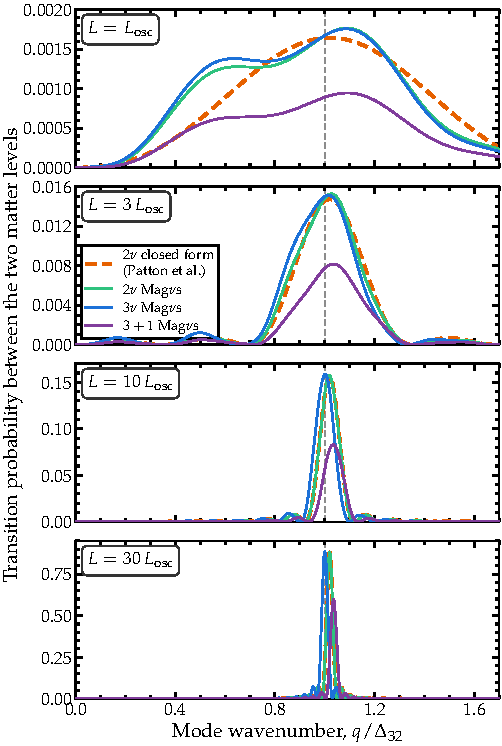
\includegraphics[width=\columnwidth]{turbulence_rabi.pdf}
 \caption{\label{fig:turbulence_rabi}Probability of transition between two matter levels coupled by a single density mode, against the wavenumber of the Fourier mode of the matter density in the medium, for a 5-GeV neutrino in a region of mean density $\rho_0 = 4$~g~cm$^{-3}$ carrying one mode of amplitude $C = 0.03$. The panels are region lengths of $1$, $3$, $10$, and $30\,L_{\rm osc}$, with $L_{\rm osc} = 2\pi/\Delta_{32} = 10\,938$~km the oscillation length driven by the 2-3 sector. The closed form of \Refs\ \cite{Patton:2013dba, Patton:2014lza}, \equ{turb_rabi}, is evaluated for the two-flavor reduction of the 1-3 sector; \magnus\ is run at two, three, and four flavors, the last with $\sin^2\theta_{14} = \sin^2\theta_{24} = 0.10$ and $\Delta m^2_{41} = 1$~eV$^2$. The levels are those of the mean density, between which no transition occurs without the mode. See notebook \#28 and Sec.~\ref{sec:turbulence} for details.}
\end{figure}
%%%%%%%%%%%%%%%%%%%%%%%%%%%%%%%%%%%%%%%%%%%%%%%%%%%%%

%%%%%%%%%%%%%%%%%%%%%%%%%%%%%%%%%%%%%%%%%%%%%%%%%%%%%
\begin{figure}[t!]
 \centering
 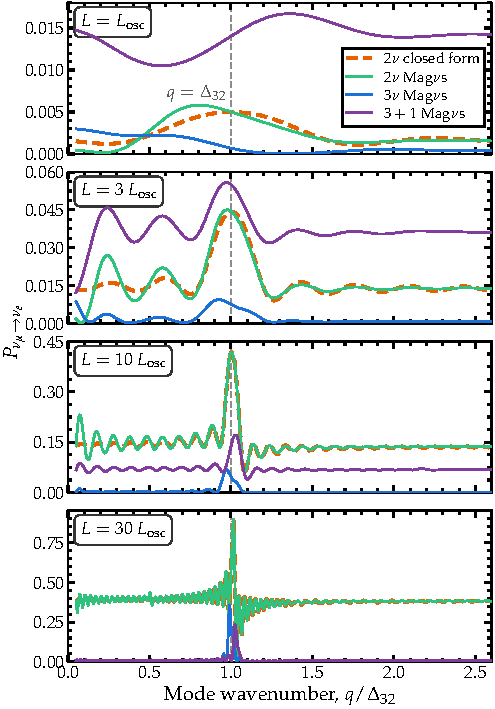
\includegraphics[width=\columnwidth]{turbulence.pdf}
 \caption{\label{fig:turbulence}Flavor transition probability $P_{\nu_\mu \to \nu_e}$ for the same neutrino, medium, mode, and region lengths as Fig.~\ref{fig:turbulence_rabi}, at two, three, and four flavors. The line labeled $q = \Delta_{32}$ marks the mode that matches the three-flavor gap; the two- and four-flavor gaps lie a few percent away from it. The curves sit at different heights because the three flavor counts give different probabilities over the same region even without the mode. The closed-form curve is \equ{turb_rw_flavor}, the flavor probability built from the propagator behind \equ{turb_rabi}, for the same two-flavor system as in Fig.~\ref{fig:turbulence_rabi}. See notebook \#28 and Sec.~\ref{sec:turbulence} for details.}
\end{figure}
%%%%%%%%%%%%%%%%%%%%%%%%%%%%%%%%%%%%%%%%%%%%%%%%%%%%%

Matter behind a supernova shock does not settle: convection keeps stirring it. Its density fluctuates around its mean value by tens of percent, over a range of length scales spanning from the size of the star to far below it\ \cite{Loreti:1995ae, Schirato:2002tg, Fogli:2006xy, Patton:2013dba, Patton:2014lza}. Therefore, an escaping neutrino meets a profile with a density that has a regular component---decreasing with distance from the center---and a random component overlaid on it. In the Fourier decomposition of that random component, a mode of wavenumber $q$ moves neutrinos between a pair of eigenstates of $\mathbb{H}$ when $q$ coincides with the eigenvalue gap $\Delta_{jk} = \lambda_j - \lambda_k$, the random density mode playing the role that an oscillating field plays in parametric resonance (Sec.~\ref{sec:order_is_the_slab_product}).

References\ \cite{Patton:2013dba, Patton:2014lza} solved that problem in closed form. Treating the random component as a perturbation on the regular one and keeping the resonant term, they obtained a Rabi formula for the transition between the two levels,
\begin{equation}
 P_{jk}
 =
 \frac{\kappa^2}{p^2 + \kappa^2}\,
 \sin^2\!\left(\sqrt{p^2 + \kappa^2}\; L\right) ,
 \qquad
 p = \tfrac{1}{2}\left(\Delta_{jk} - q\right) ,
 \label{equ:turb_rabi}
\end{equation}
where $L$ is the length of the turbulent region and $\kappa \equiv \tfrac{1}{2} C V_{\rm CC} \lvert U^m_{ej} U^m_{ek}\rvert$ is the coupling induced between the two levels by a density mode $\rho(l) = \rho_0 \left[1 + C \cos(q l)\right]$, with $\rho_0$ the mean density and $U^m$ the mixing matrix in matter. On resonance, where $q = \Delta_{jk}$, the probability is $\sin^2(\kappa L)$: the amplitude $C$ sets how long the region must be for complete conversion to occur.

As example, we consider a region of mean density $\rho_0 = 4$~g~cm$^{-3}$ carrying one mode of amplitude $C = 0.03$, crossed by a 5-GeV neutrino:
\begin{pysnip}
import numpy as np
import magnus.globaldefs as gd
import magnus.matter as matter
import magnus.hamiltonians as ham

OSC = gd.load_nufit_params('NuFIT 6.1')
E = 5.0*gd.UNIT_GEV    # Neutrino energy
RHO0 = 4.0             # Mean density, g/cm3
C = 0.03               # Mode amplitude

def one_mode(q):
    """Density along the ray: the mean, plus
    one mode of wavenumber q."""
    def rho(l):
        x = np.asarray(l, dtype=float)
        return RHO0*(1.0 + C*np.cos(q*x))
    return rho
\end{pysnip}
The gaps of the Hamiltonian at $\rho_0$ fix the range of $q$ to scan:
\begin{pysnip}
# n_e and V_CC of the smooth medium
ne0 = matter.num_density_e_func(
    0.0, lambda l: RHO0,
    density_matter_is_in_g_per_cm3=True)
V0 = matter.VCC_func(0.0, lambda l: ne0)

# H at the mean density: vacuum plus matter
H0 = np.array(ham.hamiltonian_3nu_vacuum(
    E, **OSC), dtype=complex)
H0 += ham.hamiltonian_3nu_matter(V0)

# Eigenvalues w, matter eigenvectors Vm, and
# the gap the mode has to match
w, Vm = np.linalg.eigh(H0)
d32 = abs(w[2] - w[1])
LOSC = 2*np.pi/d32     # 10 938 km
\end{pysnip}
Here, $\Delta_{32}$ is matched by a mode of wavelength $L_{\rm osc} \equiv 2\pi/\Delta_{32} = 10\,938$~km, the oscillation length of that pair of levels.

Equation~(\ref{equ:turb_rabi}) gives the transition probability between two eigenstates of $\mathbb{H}$~\cite{Patton:2013dba, Patton:2014lza}.  The same quantity is contained in the evolution operator $\mathbb{U}$ of \equ{probability}, once $\mathbb{U}$ is written in the basis of those eigenstates: $\lvert [\mathbb{U}]_{jk} \rvert^2$ is the transition probability between levels $k$ and $j$. If the density were constant, $\mathbb{H}$ would be the same at every point of the region; its eigenstates would then evolve independently of one another, so $\lvert [\mathbb{U}]_{jk} \rvert^2$ would vanish for $j \neq k$. The Fourier mode makes the density vary along the region, so $\mathbb{H}$ varies with it. In the basis of the eigenstates at $\rho_0$, that variation appears as the off-diagonal elements $C V_{\rm CC} \cos(ql)\, U^{m*}_{ej} U^m_{ek}$ of $\mathbb{H}$. Those elements mix the levels as the neutrino advances, so $\mathbb{U}$ acquires off-diagonal elements too; $\lvert [\mathbb{U}]_{jk} \rvert^2$ is what that mixing amounts to over the whole region. \magnus\ returns $\mathbb{U}$; rotating it into that basis is one line:
\begin{pysnip}
from magnus.oscprob import (
  compute_evolution_operator_multiple_slabs
  as chain)

L = LOSC             # The region, one L_osc
rho = one_mode(d32)  # Mode tuned to the gap

def H(l):
    """H at position l, with the mode on."""
    h = np.array(ham.hamiltonian_3nu_vacuum(
        E, **OSC), dtype=complex)
    # V_CC follows the density
    return h + ham.hamiltonian_3nu_matter(
        V0*rho(l)/RHO0)

# One operator per slab, then the ordered
# product over the chain
edges = np.linspace(0.0, L, 501)
slabs = np.stack([edges[:-1], edges[1:]], 1)
Us = chain(H, slabs, 9, 6)
U = Us[0]
for u in Us[1:]:     # Earliest slab first
    U = u @ U

# Rotate to the matter basis, then read the
# transition between levels 2 and 3
P32 = abs((Vm.conj().T @ U @ Vm)[2, 1])**2
P32                    # 0.001674
\end{pysnip}

Figure~\ref{fig:turbulence_rabi} compares \equ{turb_rabi} with \magnus\ at four lengths of the turbulent region; the closed form is evaluated for the two-flavor system it was derived for, the 1--3 sector, with $\kappa$ from the two-flavor $\mathbb{U}^m$ at $\rho_0$. The closed form of \Refs~\cite{Patton:2013dba, Patton:2014lza} keeps only the part of the coupling that varies slowly along the trajectory; the part it discards averages out only over many of its own cycles. One $L_{\rm osc}$ (\figu{turbulence_rabi}, top panel) contains too few of them, so the closed form and the two-flavor \magnus\ curve differ appreciably; the difference shrinks as the region lengthens (\figu{turbulence_rabi}, bottom three panels). A third or fourth flavor changes the eigenvalue gap and moves the resonance to a different wavenumber, while the length of the region sets its width: the longer the region, the more closely the mode has to match the gap. 

Figure~\ref{fig:turbulence} shows the associated oscillation probabilities $P_{\nu_\mu \to \nu_e}$, computed via
\begin{pysnip}
import magnus.oscprob as oscprob

kw = dict(
    nu_i=gd.NUMU, nu_f=gd.NUE,
    density_matter_is_in_g_per_cm3=True)

# Two flavors: the 1-3 sector
OSC2 = dict(sth=OSC['s13'], Dm2=OSC['D31'])
P2 = oscprob.osc_prob_matter_std_potential(
    2, one_mode(d32), E, L, OSC2, **kw)

# Three flavors
P3 = oscprob.osc_prob_matter_std_potential(
    3, one_mode(d32), E, L, OSC, **kw)

# The same call with a sterile state added
OSC4 = dict(OSC, s14=np.sqrt(0.10), D41=1.0,
            s24=np.sqrt(0.10), s34=0.0,
            d14=0.0, d24=0.0)
P4 = oscprob.osc_prob_matter_std_potential(
    4, one_mode(d32), E, L, OSC4, **kw)
\end{pysnip}
In \figu{turbulence}, the largest change of the probability sits around wavenumber, $q = \Delta_{32}$. This is the resonance of \figu{turbulence_rabi}, seen in the flavor channel; as there, it narrows as the region lengthens. Above $\Delta_{32}$ the curves are flat: a mode faster than every gap cancels its effect along the trajectory. 

Figure~\ref{fig:turbulence} also shows the flavor probability that follows from the closed form. Near the resonance it follows the two-flavor \magnus\ curve, more closely the longer the region. At low wavenumber it does not: there it stays at the value of the smooth medium, while \magnus\ swings above it. That curve is built as follows. Equation~(\ref{equ:turb_rabi}) is the modulus squared of one element of the propagator of the two-level system in the rotating-wave approximation, the solution behind the closed form\ \cite{Patton:2013dba, Patton:2014lza}. In the matter basis of the mean density, that propagator is
\begin{equation}
 \tilde{\mathbb{U}}(L)
 =
 {\rm diag}\!\left(e^{iqL/2}, e^{-iqL/2}\right)
 \exp\!\left[
 -i L
 \begin{pmatrix}
  \bar\lambda - p & \kappa_c \\
  \kappa_c^* & \bar\lambda + p
 \end{pmatrix}
 \right] ,
 \label{equ:turb_rw_u}
\end{equation}
where $\bar\lambda = \tfrac{1}{2}(\lambda_1 + \lambda_2)$ and $p = \tfrac{1}{2}(\lambda_2 - \lambda_1 - q)$ are the mean of the two levels and the detuning, while $\kappa_c = \tfrac{1}{2} C V_{\rm CC}\, U^{m*}_{e1} U^m_{e2}$ is the coupling, with $\lvert \kappa_c \rvert = \kappa$. The matrix in the exponent is the Hamiltonian in the frame that rotates with the mode, in which it is constant; the first factor undoes that rotation. The flavor probability reads the same propagator with flavor indices,
\begin{equation}
 P_{\nu_\mu \to \nu_e}
 =
 \left\lvert \left[ U^m\, \tilde{\mathbb{U}}(L)\, U^{m\dagger} \right]_{e\mu} \right\rvert^2 .
 \label{equ:turb_rw_flavor}
\end{equation}
The matrix in \equ{turb_rw_u} couples the two levels but does not move them: the rotating-wave approximation drops the part of the mode that raises and lowers the levels along with the density. At low wavenumber that part is all there is. Such a mode changes the density slowly; the levels follow it, with no transition driven between them. Equation~(\ref{equ:turb_rw_u}) misses that effect, so its curve stays at the value of the smooth medium at low wavenumber.

%%%%%%%%%%%%%%%%%%%%%%%%%%%%%%%%%%%%%%%%%%%%%%%%%%%%%

\subsection{Running a scan in parallel}
\label{sec:njobs}

A scan of many probabilities can be shared among processes. Every wrapper accepts the argument {\tt n\_jobs} for that, the number of processes to use, with {\tt n\_jobs = 1} as default:
\begin{pysnip}
import numpy as np
import magnus.oscprob as oscprob
import magnus.globaldefs as gd

N = 5000
E = np.logspace(-0.3, 1.3, N)*gd.UNIT_GEV
L = np.linspace(2e3, 11467.8, N)*gd.UNIT_KM
kw = dict(costhz=-0.9, rtol=1e-6, atol=1e-8,
          nu_i=gd.NUMU, nu_f=gd.NUMU)

# Every point has its own baseline, so no
# batched engine takes this scan
P = oscprob.osc_prob_3nu_earth(
    E, L=L, n_jobs=4, **kw)
\end{pysnip}

The first point in the scan runs by itself, in the main process. That run fixes the parameters. Its refinement ladder settles on two numbers: how many slabs the trajectory needs ($N_{\rm slabs}$), and how many collocation points each slab needs to evaluate the Magnus expansion. Those two numbers become the starting floor for every later point, set two rungs below where the first point landed. Each worker then begins its ladder close to the answer. The rest of the scan goes to the workers. Each worker takes a chunk of consecutive points and computes them one after another. {\tt joblib} picks the batch size, aiming for chunks that run between $0.2$ and $2$~s, so cheap points are gathered in bulk and an expensive point is handed over on its own.

Two conditions decide whether using {\tt n\_jobs} larger than 1 helps. The first is the shape of the scan. A batched engine answers only at {\tt n\_jobs} $= 1$, so asking for more processes sends the request down the per-point path instead, which for a batchable scan is the slower of the two (Sec.~\ref{sec:batching}). A scan whose points share one baseline should keep the default of {\tt n\_jobs} $= 1$ and let the batching of Sec.~\ref{sec:batched_calls} do the work:
\begin{pysnip}
# One baseline for all energies: the batched
# engine takes it, at the default n_jobs = 1
P = oscprob.osc_prob_3nu_earth(
    E, L=11467.8*gd.UNIT_KM, **kw)
\end{pysnip}
Parallelism is for scans that no batched engine accepts, such as the one above, where every energy carries a different baseline.

The second condition is length. Starting the workers costs time, paid once per call, so the scan has to be long enough to absorb this overhead. Measured on the scan above, four workers return $2.4$ times the speed of one process at $5\,000$ points, $2.3$ at $2\,000$ and $1.8$ at $500$. A scan of a few hundred points called once can finish slower than it would have in a single process. Section~\ref{sec:cost} and \figu{njobs_scaling} measure how that gain grows with the size of the scan and where it stops paying.

Parallelism changes more than the speed. A serial scan warm-starts each point from its neighbor. A parallel scan warm-starts every point from the first one. A ladder that starts on a different rung can stop on a different rung, so two runs that differ only in {\tt n\_jobs} agree to the tolerance asked for, but no better. The gap between grows with the length of the scan. Measured on the chord above at {\tt rtol} $= 10^{-6}$, two points agree exactly, three differ by $8 \cdot 10^{-10}$, and forty by $10^{-8}$. The user should hold {\tt n\_jobs} fixed when two runs have to match to the last digit.

All of the above concerns a scan of several probabilities, which is the only thing {\tt n\_jobs} affects. A call for a single probability accepts it and ignores it. The slabs of one calculation go to the batched kernel in a single call, and no worker is started:
\begin{pysnip}
# Many points: each worker receives points
P = oscprob.osc_prob_3nu_earth(
    E, L=L, n_jobs=4, **kw)

# One point: n_jobs is accepted and does
# nothing; the call runs in one process
P = oscprob.osc_prob_3nu_earth(
    10.0*gd.UNIT_GEV, L=11467.8*gd.UNIT_KM,
    n_jobs=4, **kw)
\end{pysnip}
(Distributing slabs was tried and retired. A slab is far smaller than a probability, and evaluating all of them in one batched call beats handing them out one at a time.) 

%%%%%%%%%%%%%%%%%%%%%%%%%%%%%%%%%%%%%%%%%%%%%%%%%%%%%

\subsection{Using \magnus\ from the command line}
\label{sec:cli}

\magnus\ installs a console script, {\tt magnus}, that computes a single probability, or a probability matrix, without writing any Python; {\tt python -m magnus} runs the same program. Its {\tt prob} subcommand selects a wrapper of Section \ref{sec:scope_interface} from three options, {\tt --flavors}, {\tt --environment}, and {\tt --scenario}, and takes the physical parameters as options of the same names as the wrapper's arguments, with the oscillation parameters defaulting to the NuFIT 6.1 values. For the Earth, the baseline may be given directly, together with the arrival direction, or computed from two named locations. The refinement keywords of Section \ref{sec:architecture} are available as options as well. Listing~\ref{lst:cli} shows two calls: the constant-density probability matrix of Listing~\ref{lst:constant}, and the $\nu_\mu \to \nu_e$ probability along the chord from Fermilab to Homestake. The documentation site\ \cite{MagnusDocs} lists every option.

%%%%%%%%%%%%%%%%%%%%%%%%%%%%%%%%%%%%%%%%%%%%%%%%%%%%%
\begin{lstlisting}[language=bash, caption={Two probabilities from the command line. The first is the matrix of Listing~\ref{lst:constant}; the second is one channel along a chord through the Earth, with the baseline computed from the two named locations. The mixing parameters take their NuFIT 6.1 defaults.}, label={lst:cli}, float=tbp]
$ magnus prob --flavors 3 --environment matter \
    --density-profile constant --rho 3.0 \
    --energy 1 --baseline 1000
Magnus 1.1.1 -- osc_prob_3nu_matter_constant_density
E = 1 GeV, L = 1000 km

            nu_e   nu_mu  nu_tau
nu_e      0.9855  0.0134  0.0012
nu_mu     0.0135  0.9864  0.0001
nu_tau    0.0011  0.0002  0.9987

$ magnus prob --flavors 3 --environment earth \
    --loc-ini fermilab --loc-fin homestake \
    --energy 2.5 --nu-i mu --nu-f e
Magnus 1.1.1 -- osc_prob_3nu_earth
E = 2.5 GeV

P = 0.0722
\end{lstlisting}
%%%%%%%%%%%%%%%%%%%%%%%%%%%%%%%%%%%%%%%%%%%%%%%%%%%%%

The script also exposes the numerical options of Sec.~\ref{sec:architecture}. {\tt --rtol} and {\tt --atol} set the tolerance, {\tt --strategy} asks for one of the routes of Sec.~\ref{sec:engines}, {\tt --magnus-exp-order} sets the order of the expansion, {\tt --n-jobs} spreads the work over several workers. Both tolerances default to $10^{-3}$ here, looser than the setting behind every figure in this paper, so a number from the command line can differ from a plotted one in the third digit.

Listing~\ref{lst:cli_json} shows that adding {\tt --json} prints the same result as a JSON object, making it ready for a script that is part of a bigger pipeline. Two cases require the baseline explicitly. Through the Earth, {\tt --costhz} fixes the direction of the chord but not its length, so it needs {\tt --baseline} beside it. Only the pair {\tt --loc-ini} and {\tt --loc-fin} works out the length on its own. The Sun likewise needs an explicit {\tt --baseline}.

%%%%%%%%%%%%%%%%%%%%%%%%%%%%%%%%%%%%%%%%%%%%%%%%%%%%%
\begin{lstlisting}[language=bash, caption={The same probability as in Listing~\ref{lst:cli}, but returned as JSON. The object names the function that computed it, the configuration behind it, the inputs in natural units.}, label={lst:cli_json}, float=tbp]
$ magnus prob --flavors 3 --environment matter \
    --density-profile constant --rho 3.0 \
    --energy 1 --baseline 1000 \
    --nu-i mu --nu-f e --json
{
  "function": "osc_prob_3nu_matter_constant_density",
  "flavors": 3,
  "environment": "matter",
  "scenario": "std",
  "nubar": false,
  "energy_eV": 1000000000.0,
  "baseline_eV-1": 5067730000000.0,
  "probability": 0.013475467612077624
}
\end{lstlisting}
%%%%%%%%%%%%%%%%%%%%%%%%%%%%%%%%%%%%%%%%%%%%%%%%%%%%%

The console script computes one probability at a time. It takes one energy and one baseline. It offers no scan, no averaged probability, no way to read a density profile from a file, no way to supply a Hamiltonian of one's own. Those belong in Python, through the calls of the sections above. The script is for a quick number, for a check against another code, or for a probability inside a shell pipeline.

%%%%%%%%%%%%%%%%%%%%%%%%%%%%%%%%%%%%%%%%%%%%%%%%%%%%%
%%%%%%%%%%%%%%%%%%%%%%%%%%%%%%%%%%%%%%%%%%%%%%%%%%%%%

\section{Performance, precision, and reach}
\label{sec:performance}

%%%%%%%%%%%%%%%%%%%%%%%%%%%%%%%%%%%%%%%%%%%%%%%%%%%%%

\subsection{Timing measurement protocol}
\label{sec:timing_protocol}

Every timing in this paper---this section, Sec.~\ref{sec:comparison}, and every other cost quoted---comes from one machine and one software stack: a 13th-generation Intel Core i5-1334U with 16~GB of memory, running Ubuntu 24.04 LTS on Linux kernel 7.0.0, with Python 3.12.7, {\tt NumPy} 1.26.4, and \magnus\ 1.1.1. The timings of the other codes in Figs.~\ref{fig:prem_plane} and \ref{fig:shock_cost} come from the benchmark suite of {\tt NuOscProbExact}~\cite{Bustamante:2019ggq, NuOscProbExact}, run on the same machine under that suite's own protocol.control ratio of the run.

Absolute times mean little on their own; we quote ratios whenever possible. A comparison of two code paths in \magnus---or two codes---runs on a harness that interleaves them round-robin and carries a control workload the change cannot touch. A factor of two or more in run times between two codes is a property of the codes and survives a change of machine; a factor of a few percent belongs to the machine.

Two features of the protocol keep one-off costs out of the measurement; without them, \magnus\ would look slow for reasons unrelated to how it computes. The first is a warm-up pass. The first call on a machine compiles the {\tt Numba} kernels, which takes about 2~s, far longer than computing a grid of twelve energies. Compiled kernels are cached on disk, but each later session still spends about 0.1~s loading them on first call. Therefore, we discard the first call and start timing from the second.

The second is an adaptive repeat count. We time a setting by calling it many times in one block and dividing by the number of calls; too few calls leave the block so short that the timer's resolution and background jitter dominate. The number of calls therefore grows until the block lasts at least 50~ms. We take three such blocks per point and report the fastest. Where we check it, the coefficient of variation across the three---the standard deviation over the mean---stays below 0.10.

%%%%%%%%%%%%%%%%%%%%%%%%%%%%%%%%%%%%%%%%%%%%%%%%%%%%%

\subsection{Slab width follows the profile, not the phase}
\label{sec:phase_vs_profile}

%%%%%%%%%%%%%%%%%%%%%%%%%%%%%%%%%%%%%%%%%%%%%%%%%%%%%
\begin{figure*}[t!]
 \centering
 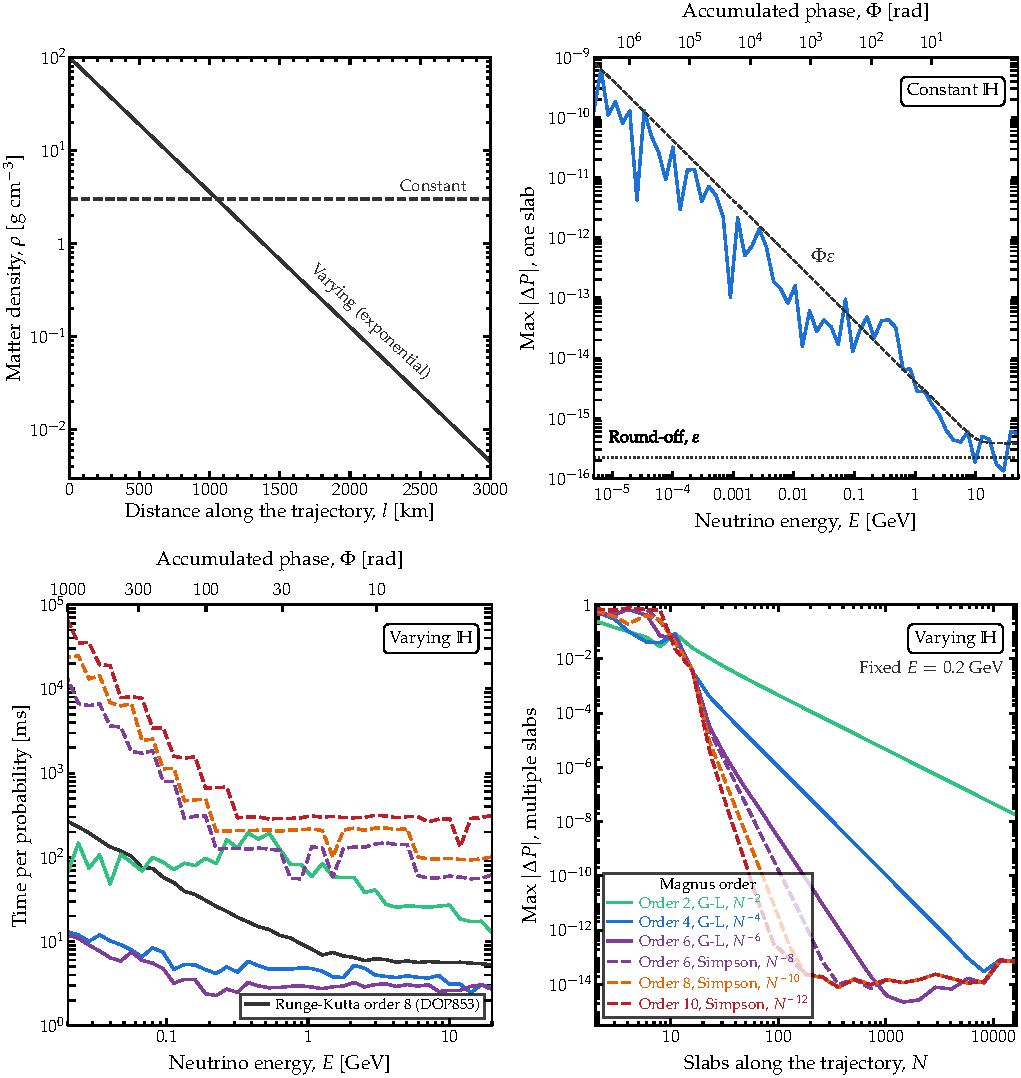
\includegraphics[width=\textwidth]{phase_vs_profile.pdf}
 \caption{\label{fig:phase_vs_profile}\textbf{Cost and accuracy of a Magnus slab, at three flavors.} \emph{Top left}: the two matter-density profiles, both at an electron fraction of 0.5. The constant 3~g~cm$^{-3}$ is used in the top-right panel; the exponential, of central density 100~g~cm$^{-3}$ and scale height 300~km, in the bottom panels. \emph{Top right}: deviation of one slab from an exact exponentiation of the same constant $\mathbb{H}$, against energy, with the accumulated phase $\Phi$ of \equ{phase} on the upper axis. The series terminates at $\Omega_1$, so only arithmetic remains: the deviation bottoms out near machine epsilon, $\varepsilon = 2.2 \cdot 10^{-16}$, and rises along $\Phi\varepsilon$. \emph{Bottom left}: time per probability for the six Magnus configurations and for {\tt DOP853}, which is timed alongside them and is not the reference. All run at a tolerance of $10^{-8}$, with the slab count and the samples per slab chosen by the package. Cost climbs in steps because the code refines in discrete stages. The worst deviations from the reference range from $2.4 \cdot 10^{-7}$ for {\tt DOP853} to $1.5 \cdot 10^{-11}$ for order 10. \emph{Bottom right}: deviation from the reference against the number of slabs, at 0.2~GeV. Every reference is Richardson-extrapolated three times in extended precision: at fifty decimal digits for the right-hand panels, converged to $3 \cdot 10^{-20}$, and at thirty digits, one solution per energy, converged past $10^{-11}$, for the bottom-left panel. See Sec.~\ref{sec:phase_vs_profile} for details.}
\end{figure*}
%%%%%%%%%%%%%%%%%%%%%%%%%%%%%%%%%%%%%%%%%%%%%%%%%%%%%

Figure~\ref{fig:phase_vs_profile} measures what sets the width of a slab: the density profile, not the oscillation phase. \magnus\ makes each slab narrow enough that the density changes little across it, however many oscillations fall inside. So its cost follows the profile, while that of a step-by-step solver grows with the number of oscillations, since it must resolve them.

The top-left panel of \figu{phase_vs_profile} shows the two density profiles used in this benchmarking: a constant 3~g~cm$^{-3}$ and an exponential of central density 100~g~cm$^{-3}$ with a 300-km scale height. The top-right panel holds the Hamiltonian constant and measures the error of a single slab as the phase across it grows. The bottom-left panel sweeps the energy along the exponential profile and times one probability at a fixed tolerance. Finally, the bottom-right panel fixes the energy and follows the error down against the slab count. We elaborate on these below.

\smallskip

\textit{Reference probability.---}We score the probabilities computed by \magnus\ against a reference that is far more accurate than any of them. The reference cuts the path into equal-width slabs, reads the density at the midpoint of each, and multiplies the exponentials together. We compute the reference in extended precision with {\tt mpmath}, so rounding errors do not affect it. The reference still depends on the number of slabs. We remove that dependence by Richardson extrapolation. Doubling the slab count shrinks the leading error term by a known factor, so combining two runs cancels that term. Three successive combinations cancel the three largest terms. We keep doubling until the last two extrapolated values agree within a set threshold; their difference is the reference's error. The right-hand panels use fifty digits, because their deviations reach the double-precision round-off near $10^{-16}$; the reference there converges to about $10^{-20}$. The bottom-left panel needs only $10^{-11}$ but a separate reference at each energy of the sweep, so we use thirty digits there. 

\smallskip

\textit{Why the sweep is in energy.---}The accumulated phase, \equ{phase}, is set by the eigenvalue gap of $\mathbb{H}$. In \figu{phase_vs_profile}, its vacuum part scales as $1/E$ and its matter part does not (see Sec.~\ref{sec:recap}), so lowering the energy raises the phase while leaving the density profile untouched. That is what makes an energy sweep a test of the two against each other: one quantity moves and the other does not. The phase does not scale purely $\propto 1/E$: across the bottom-left panel, from 20 to 0.02~GeV, a factor of a thousand in energy carries $\Phi$ from 6 to 952 radians, a factor of about 150, because the energy-independent matter term dominates the gap at the high-energy end. Each panel in \figu{phase_vs_profile} carries $\Phi$ on a second axis above the energy.

\smallskip

\textit{A constant Hamiltonian costs one slab.---}If $\mathbb{H}$ does not depend on position, $l$, then every commutator in \equ{recursion} vanishes identically, $\Omega = -i\mathbb{H}\Delta l$ exactly, so the expansion terminates at its first term. The evolution operator over the whole interval is one exponential, whatever the accumulated phase. The upper-right panel of \figu{phase_vs_profile} tests this over six decades of phase. What grows is $\Phi\varepsilon$, with $\varepsilon$ the double-precision unit round-off, which reaches about $10^{-9}$. That is the accuracy with which the phase is representable. It has nothing to do with the Magnus expansion: a closed-form probability~\cite{Bustamante:2019ggq} evaluated in double precision at the same phase carries the same accuracy. At the top of that span, a double-precision exponentiation is itself in error by about $10^{-10}$, the same size as the deviation being measured, so a double-precision reference could not tell the two apart. This is why we carry the reference at fifty decimal digits.

\smallskip

\textit{A varying Hamiltonian costs more.---}The corrections $\Omega_2, \Omega_3, \ldots$ in \equ{recursion} are built from commutators of $\mathbb{A}$ at two different positions. Each commutator is small when $\mathbb{A}$ changes little between those positions. Therefore, a slab should ideally be narrow enough that the \emph{Hamiltonian}---and not necessarily the neutrino state---is nearly constant across it. 

Inside a slab, the neutrino state and the Hamiltonian change at different rates. The state oscillates, rotating through $\Phi$ radians, while the Hamiltonian changes only as fast as the matter density, which can be far slower. A traditional solver that advances the state in steps (like {\tt DOP853} below) must keep each step shorter than an oscillation period, so its cost grows with the phase. \magnus\ instead integrates the Hamiltonian over the slab, which involves no oscillation; the exponential of the result produces all $\Phi$ radians at once. So the slab width is set by how fast $\mathbb{H}$ varies, not by how many oscillations fall inside the slab. Both codes are timed returning the full evolution matrix. For {\tt DOP853}, that means integrating all initial flavors together in a single run, which is faster than integrating them one at a time.

The bottom-left panel of \figu{phase_vs_profile} shows what that difference costs. We compare \magnus\ against a stand-alone Runge-Kutta order-8 solver, the \texttt{DOP853} algorithm as implemented in \texttt{scipy.integrate}. We score both against the extended-precision reference described above. Along the exponential profile, we sweep the energy from 20 to 0.02~GeV, which raises the accumulated phase from 6 to 952 radians. Every configuration, {\tt DOP853} included, runs at a tolerance of $10^{-8}$. \magnus\ chooses the slab count and the samples per slab from that tolerance, as in normal use. Its refinement proceeds in discrete stages, so its cost rises in steps; each jump marks a new stage. The panel shows:
\begin{itemize}
\item \textit{Cost follows the profile, not the phase.} Over the sweep, the phase grows about 150-fold. The time per probability of {\tt DOP853} grows 50-fold, from about 5 to 270~ms. That of \magnus\ at orders 4 and 6 on Gauss-Legendre (G-L) grows only 4-fold, from under 3 to 12--13~ms. The gap between the two widens from 2 to about 20.
%%%%
\item \textit{\magnus\ is also more accurate.} A tolerance is a request, not a guarantee. Asked for $10^{-8}$, {\tt DOP853} returns up to $2 \cdot 10^{-7}$. Every Magnus configuration stays below $10^{-8}$, order 10 by nearly three orders of magnitude. At the low-phase end, the highest orders fall below the reference's own error, so we can say only that they match it.
%%%%
\item \textit{The slab count is set by the profile.} At low phase, both codes stop responding to the phase. On the exponential profile, the order-6 slab count stays at about 160 while the phase grows sixfold, up to 36 radians. A different profile changes it at the same phase: a constant density needs 2 slabs, and an exponential ten times flatter needs 72. {\tt DOP853} behaves the opposite way: a steeper profile holds less matter along the path, so it carries less phase, and {\tt DOP853} takes \emph{fewer} steps.
%%%%
\item \textit{Low order pays at resonances.} Order-2 Magnus is the slowest G-L configuration (Sec.~\ref{sec:quadrature}). It converges only as $N_{\rm slabs}^{-2}$, so it needs thousands of slabs at any phase. The hump in its curve is the $\Delta m^2_{31}$ MSW resonance, which the path crosses at intermediate energies. Below about 0.31~GeV, the resonant density exceeds the profile's central 100~g~cm$^{-3}$, so the resonance disappears. Near it, $\mathbb{H}$ changes fastest and the slabs must narrow. Magnus orders 4 and 6 absorb that change with their higher-order terms, so they feel it far less, yielding shallower humps.
%%%%
\item \textit{Simpson's rule needs many more samples.} The Simpson configurations of Sec.~\ref{sec:quadrature}, at orders 6, 8, and 10, cost the most. Their slab counts track the phase like the G-L counts, but their samples per slab grow from about 60 to a ceiling of 500, while G-L keeps 2. At the high-phase end, order 10 on Simpson evaluates $\mathbb{H}$ some $4 \cdot 10^{5}$ times, taking about a minute per probability. Order 6 on Gauss-Legendre evaluates it 3\,000 times, in about 12~ms.
\end{itemize}

\smallskip

\textit{The round-off floor.---}In the bottom-right panel of \figu{phase_vs_profile}, the error first falls as slabs are added, then stops falling. Two errors compete. The truncation error falls as $N_{\rm slabs}^{-p}$ at order $p$. The round-off error grows with $N_{\rm slabs}$, because every slab adds one more double-precision matrix product. Their sum is smallest, between $10^{-15}$ and $10^{-14}$, at a few hundred slabs at order 10 and several thousand at order 4. Order 2 never gets there within the slab counts shown. Past that minimum, more slabs make the answer worse, and the error climbs back toward $10^{-13}$. The refinement ladder cannot detect the floor: it stops once refining no longer changes the probability, and near the floor refining no longer changes it. Therefore, a tolerance below the floor is reported as met without being reached. Section~\ref{sec:smooth_comparison} meets the same limit in a cross-code comparison.

%%%%%%%%%%%%%%%%%%%%%%%%%%%%%%%%%%%%%%%%%%%%%%%%%%%%%

\subsection{What a probability costs}
\label{sec:cost}

%%%%%%%%%%%%%%%%%%%%%%%%%%%%%%%%%%%%%%%%%%%%%%%%%%%%%
\begin{figure}[t!]
 \centering
 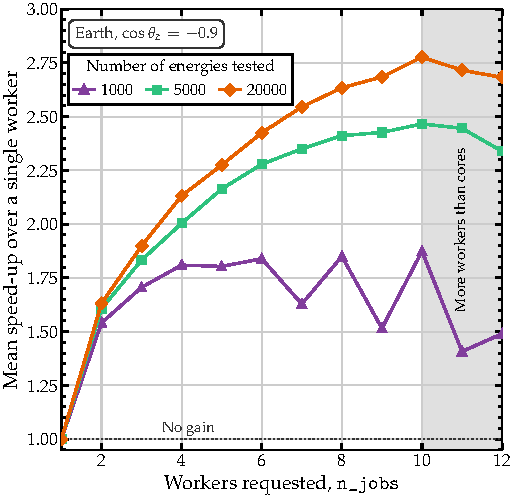
\includegraphics[width=\columnwidth]{njobs_scaling.pdf}
 \caption{\label{fig:njobs_scaling}\textbf{Parallel speed-up of an energy scan.} Speed-up against the number of worker processes, {\tt n\_jobs}, for scans of 1\,000, 5\,000, and 20\,000 energies from 0.5 to 20~GeV along an Earth chord at $\cos\theta_z = -0.9$. Each energy has its own baseline, which no batched engine accepts, so every run takes the same per-point path and the speed-up reflects the parallelism alone. Each point is the mean wall-clock time over interleaved rounds---30 at 1\,000 energies, 5 at the larger sizes---with one thread per process and the worker pool started before timing. The shaded region marks requests beyond the machine's ten physical cores (two performance, eight efficiency). Ten workers give speed-ups of $1.9\times$, $2.5\times$, and $2.8\times$ as the scan grows. The two larger sizes were measured with the worker counts in a fixed order; at 1\,000 energies, that order raised the ten-worker speed-up from $1.87\times$ to $2.23\times$, so the larger sizes may be overestimated by a similar margin. See Sec.~\ref{sec:cost} for details.}
\end{figure}
%%%%%%%%%%%%%%%%%%%%%%%%%%%%%%%%%%%%%%%%%%%%%%%%%%%%%

A single three-flavor probability through the Earth takes about 2~ms at the default tolerance of {\tt rtol} = {\tt atol} = $10^{-3}$. Across 164 Earth and solar configurations---two to five flavors, standard and non-standard Hamiltonians, neutrinos and antineutrinos---the median call takes 2~ms and the slowest under a second. A scan of many points usually costs far less than the same points computed one at a time.

Four features set that cost. The user controls three of them; \magnus\ applies the fourth automatically:
\begin{enumerate}
%%%%
\item \emph{Pass arrays.} (User's decision; \magnus\ implements it.) Every wrapper accepts an array of energies, an array of baselines, or both. \magnus\ then shares work across the points instead of starting afresh at each. For many energies at one baseline, the energy-batched engine of Sec.~\ref{sec:engines} samples the density profile once for the whole scan. For many baselines at one energy, the cumulative engine computes all of them in a single pass. Where the potential does not vary along the path, the constant-Hamiltonian engine computes the whole scan as one batch of matrix exponentials. Against the same points computed one at a time, this is worth about an order of magnitude at two and three flavors. At four and five flavors it is worth several-fold, since the exponential goes through an eigensolver instead of the closed-form kernel of Sec.~\ref{sec:exponential}. Batched answers agree with point-by-point ones to about the requested tolerance.
%%%%
\smallskip
%%%%
\item \emph{Write the Hamiltonian to accept an array of positions.} (User's decision.) A user who supplies $\mathbb{H}(l)$ decides how it is evaluated. Written to take a single position, it is called in a Python loop, once at every quadrature node of every slab; \magnus\ then issues a {\tt ScalarHamiltonianWarning}. Written to take an array of positions and return a stack of matrices---a \textit{vectorized} function, in Python terms---it is called once per refinement stage, for all slabs together. On a three-flavor exponential profile, the second form is several times faster, with identical output. It is the largest speed-up under the user's control. Section~\ref{sec:lri_sun} shows a Hamiltonian written this way.
%%%%
\smallskip
%%%%
\item \emph{Symmetry of Earth chords.} (Automatic.) A neutrino crossing a spherically symmetric Earth, such as the PREM, meets every radius twice: once on the way in and once on the way out. Therefore, the Hamiltonian along the second half of the chord repeats the first half in reverse. \magnus\ evaluates it on the first half only and mirrors it for the second. This saves only the evaluations of the Hamiltonian; the exponentials and the commutators are computed as before, since their order matters. For a plain PREM density lookup, which is cheap, the saving is negligible. For an expensive Hamiltonian, it can make the call about 1.5 times faster. \magnus\ infers the symmetry from the geometry of the chord rather than detecting it, since detecting it would require the very evaluations it saves.
%%%%
\smallskip
%%%%
\item \emph{Ask for worker processes where no batched engine applies.} (User's decision; \magnus\ implements it.) The {\tt n\_jobs} argument distributes the requested points over several processes, as described in Sec.~\ref{sec:batching}.

Figure~\ref{fig:njobs_scaling} shows the resulting speed-up against the number of processes, at three scan sizes, along an Earth chord on which every energy has its own baseline. No batched engine accepts that request, so the single-process and multi-process runs take the same per-point path; their ratio isolates the effect of parallelism. With {\tt n\_jobs} $=$ 10, the run is 2 to 3 times faster, more so for larger scans, but far from ten times. Asking for more processes than the benchmarking machine's ten physical cores brings no further gain.

More often, the whole scan shares one baseline. There, the batched engine answers only with {\tt n\_jobs} $=$ 1; any larger value sends the request to the per-point path, computed in parallel. On a scan of 5\,000 energies, that parallel run was about ten times slower than the batched call in one process. Thus, one process is the right default.
\end{enumerate}

The refinement ladder works against these savings: it computes every slab count below the one that converges, then discards those results. On an Earth chord, this makes a call about four times slower than one given the right slab count in advance. Section~\ref{sec:refinement} shows how to pass that count directly.

%%%%%%%%%%%%%%%%%%%%%%%%%%%%%%%%%%%%%%%%%%%%%%%%%%%%%

\subsection{Precision, accuracy, and tolerance}
\label{sec:diagnostics}

Precision is limited by rounding and accuracy by the refinement's stopping rule; tolerance is the user's setting for the rule.

\smallskip

\textit{Precision.---}Precision is how closely \magnus\ agrees with itself. Calling \magnus\ twice with the same inputs returns the same number bit for bit, and the test suite requires exact equality there rather than agreement within a tolerance, so a code change that let one call affect the next, through a cache for example, would fail it. A parallel run agrees with a serial one only to the requested tolerance, since each starts its refinement from a different point. With the slab grid fixed, a batched scan and the same points computed one at a time agree to $10^{-14}$. Left to refine adaptively, the two stop at different slab counts and differ at the level of the requested tolerance. The two matrix-exponential backends of Sec.~\ref{sec:exponential} agree to about $10^{-15}$ for a single exponential. On a solar profile that chains about 34\,000 of them, they differ by $3 \cdot 10^{-12}$. That is within the $N_{\rm slabs}\,\varepsilon = 7.4 \cdot 10^{-12}$ that rounding can accumulate over that many double-precision products, with $\varepsilon$ the machine epsilon.

\smallskip

\textit{Accuracy.---}Accuracy is how close \magnus\ comes to the true probability. Section~\ref{sec:validation} measures it against external references. The actual error can differ from the requested tolerance in either direction. At the default {\tt rtol} $=$ {\tt atol} $= 10^{-3}$, a probability through the Earth is usually much more accurate than $10^{-3}$; in the rare cases where it is not, the error stays within about twice the tolerance. We tested this on eight Earth chords, from grazing to core-crossing, at six energies between 0.5 and 20~GeV, comparing each default result with the same call at a tolerance of $10^{-7}$. The median difference is about $10^{-6}$; nine cases in ten differ by less than $10^{-4}$. The largest difference, roughly $10^{-3}$, is on the core-crossing chord at 0.5~GeV.

That accuracy is already far better than a typical oscillation analysis needs. Such an analysis evaluates the probability on a grid---\eg, in energy and arrival direction for an atmospheric experiment, in energy alone for an accelerator experiment---interpolates between the nodes, then folds the result with a flux, a cross section, and a detector response. The error from the grid and its interpolation is orders of magnitude larger than anything the oscillation code contributes\ \cite{IceCube:2018ikn}. A code accurate to $10^{-13}$ and one accurate to $10^{-6}$ return the same answer once both have passed through that chain.

Regardless, higher accuracy is still useful. It makes \magnus\ a reference against which another code, or a coarser setting of \magnus\ itself, can be checked. Where no closed-form probability exists, it is often the only reference available. It matters for quantities computed once rather than averaged over bins, as in Secs.~\ref{sec:sun} and \ref{sec:astro}. It also separates the error of a method from the error of a model, which Sec.~\ref{sec:comparison} relies on throughout. We report the accuracy \magnus\ can reach for these uses, not because a fit to oscillation data requires it.

\smallskip

\textit{Tolerance.---}The tolerance is a stopping rule: the refinement stops once successive answers agree within it. It is not a guarantee that the answer is that close to the true value. To judge whether an answer can be trusted, the user should check the warnings \magnus\ issues. (They are standard Python warnings. By default, each message is shown once per session; {\tt warnings.simplefilter('always')} shows every occurrence, and filtering on {\tt ToleranceNotAchievedWarning} catches every warning that an answer may be outside tolerance.)

The warnings err on the side of caution: they often fire on answers that prove accurate, because most of them flag a property of the input, such as a density jump, rather than predict the error. Less often, an answer is inaccurate and no warning fires. Two successive slab counts can be wrong by the same amount and still agree, so the ladder stops with an answer outside the tolerance and no warning. Section~\ref{sec:validation} calls this a silent miss. On randomly generated smooth profiles---the hardest family we tested---about one answer in twenty-five was a silent miss.

%%%%%%%%%%%%%%%%%%%%%%%%%%%%%%%%%%%%%%%%%%%%%%%%%%%%%

\subsection{Accuracy and speed: smooth density profile}
\label{sec:smooth_comparison}

%%%%%%%%%%%%%%%%%%%%%%%%%%%%%%%%%%%%%%%%%%%%%%%%%%%%%
\begin{figure*}[t!]
 \centering
 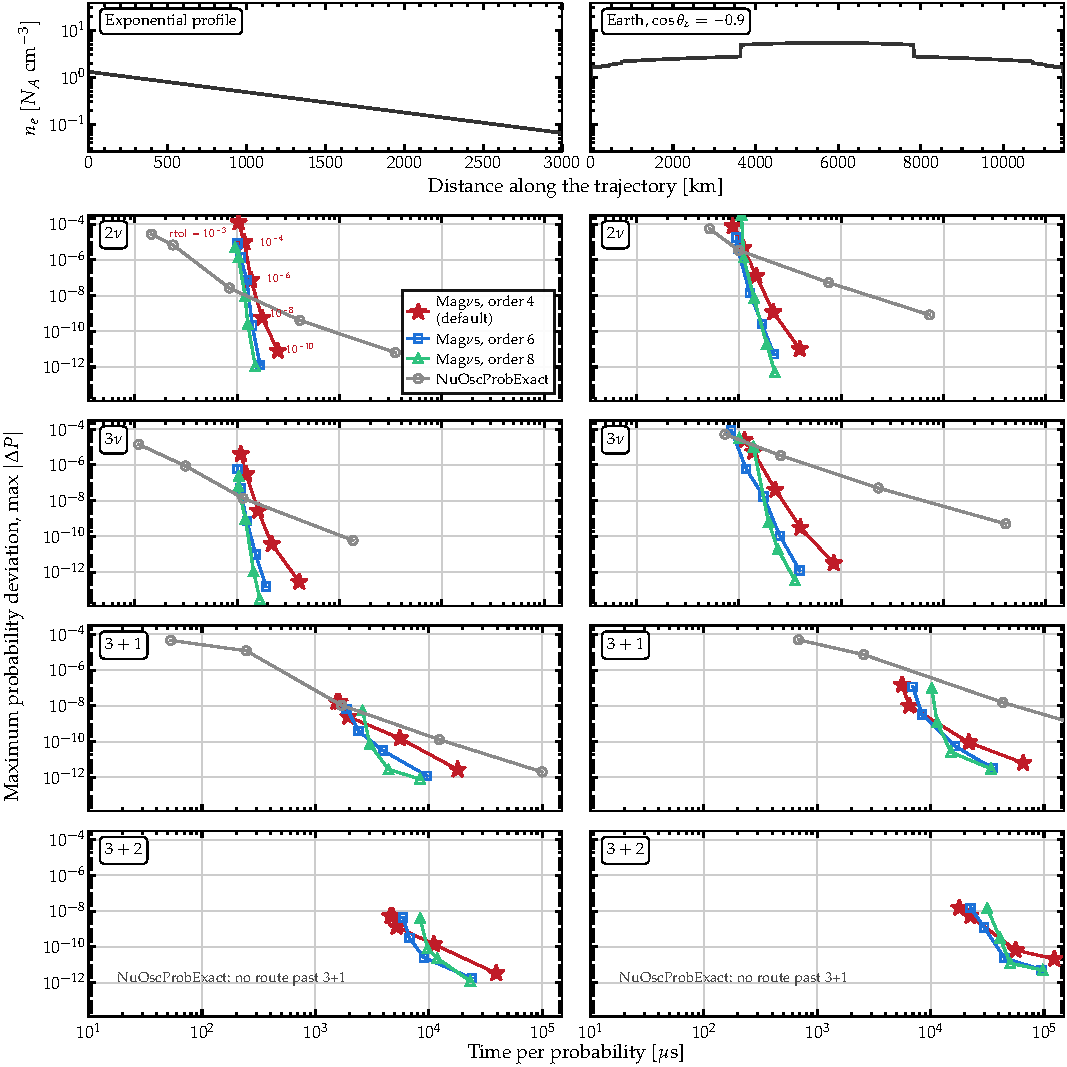
\includegraphics[width=\textwidth]{smooth_reach.pdf}
 \caption{\label{fig:smooth_reach}\textbf{Accuracy against cost, compared with {\tt NuOscProbExact}.} Deviation of the computed probability from a reference, $\lvert \Delta P \rvert$, against the time per probability, at two to five flavors, on two density profiles. \emph{Left}: a smooth exponential profile, as in the Sun. \emph{Right}: a core-crossing Earth chord at $\cos\theta_z = -0.9$, along which the PREM profile crosses sixteen layer boundaries; each boundary is passed to \magnus\ as a slab edge. The top row shows the two profiles. Both codes are scored against the same reference, computed in extended precision with {\tt mpmath} and Richardson-extrapolated. Each curve is dialed by a requested tolerance, {\tt rtol}: \magnus\ at orders 4, 6, and 8, and {\tt NuOscProbExact}\ \cite{NuOscProbExact} through its own adaptive refinement. Both codes were timed in one process on one machine (Sec.~\ref{sec:timing_protocol}). Both codes and the reference use a uniform electron fraction $Y_e = 0.5$, the default of {\tt NuOscProbExact}, in place of \magnus's layered one inside the Earth. The bottom row has no {\tt NuOscProbExact} curve, since that code stops at four flavors. See notebook \#28 and Sec.~\ref{sec:smooth_comparison} for details.}
\end{figure*}
%%%%%%%%%%%%%%%%%%%%%%%%%%%%%%%%%%%%%%%%%%%%%%%%%%%%%

Figure~\ref{fig:smooth_reach} compares \magnus\ with {\tt NuOscProbExact}\ \cite{NuOscProbExact, Bustamante:2019ggq} at two to five flavors, plotting the deviation from the reference against the time per probability. We compare against {\tt NuOscProbExact} because, among the codes of Sec.~\ref{sec:relation}, it is the one that accepts the same arbitrary Hamiltonians at two to four flavors and, like \magnus, composes the evolution from slabs; Sec.~\ref{sec:comparison} compares a wider set of codes on the Earth. 

\magnus\ is called as
\begin{verbatim}
 P = oscprob.osc_prob_matter_std_potential(
    d, ne_of, E, baseline, osc, L0=0.0,
    nu_i=gd.NUMU, nu_f=gd.NUMU,
    density_is_of_number_of_electrons=True,
    magnus_exp_order=4,
    rtol=r, atol=r*1.0e-2)
\end{verbatim}
with {\tt d} the number of flavors, {\tt ne\_of} the electron density along the trajectory, and {\tt r} the requested tolerance, swept from $10^{-3}$ to $10^{-10}$. Orders 6 and 8 differ only in {\tt magnus\_exp\_order}. On the Earth chord, the call also passes the sixteen PREM layer crossings as {\tt t\_breakpoints}. The closed form of {\tt NuOscProbExact} is the cheaper code at loose tolerances. At tight tolerances it runs into an accuracy floor that more slabs cannot lower; \magnus\ reaches past it. 

(We call the general matter \magnus\ scenario function rather than the Earth wrapper, so that the same call serves both profiles and, on each, \magnus, {\tt NuOscProbExact}, and the reference read the same electron-density function. On the Earth chord, the call passes the sixteen layer crossings as {\tt t\_breakpoints}, as the Earth wrapper would do by itself. Calling the Earth wrapper instead, with {\tt electron\_fraction=0.5}, returns the same probabilities to $10^{-15}$ at the same cost.)

\smallskip

\textit{The floor.---}As in Sec.~\ref{sec:phase_vs_profile}, composing many slab operators accumulates round-off, so past some tens of thousands of slabs the total error stops falling. At three flavors on the exponential profile, {\tt NuOscProbExact} levels off near $10^{-11}$ and cannot confirm convergence at a requested $10^{-10}$. Section~\ref{sec:shock_comparison} shows the same effect past its turning point, where more slabs make the error rise again. This happens in any long product of matrices evaluated in floating point; it is not a defect of {\tt NuOscProbExact}. \magnus\ meets the same floor 10--100 times lower, depending on the order, because a higher-order rule reaches a given accuracy with far fewer factors.

\smallskip

\textit{The ceiling.---}Adding flavors limits the two codes differently. The SU($n$) construction of {\tt NuOscProbExact}, with $n$ the number of flavors, needs the eigenvalues of the Hamiltonian from its characteristic polynomial, which is solvable in radicals only up to degree four. {\tt NuOscProbExact} has no five-flavor route, so the bottom row of \figu{smooth_reach} has no closed-form curve. \magnus\ has no such limit. At four and five flavors, its curve is flat between requested tolerances of $10^{-3}$ and $10^{-4}$: both requests return the same answer, already orders of magnitude more accurate than either asks for. From $10^{-6}$ on, each tighter request returns a smaller error, as at two and three flavors.

\smallskip

\textit{Where \magnus\ becomes faster.---}{\tt NuOscProbExact} is faster at loose tolerances, \magnus\ at tight ones. At three flavors, the curves cross at a requested tolerance between $10^{-6}$ and $10^{-8}$ on the exponential profile, and between $10^{-3}$ and $10^{-4}$ on the Earth chord. \magnus\ wins by needing fewer slabs, not cheaper ones: at two flavors, one of its order-4 slabs, run in compiled kernels, costs about four times a closed-form slab~\cite{Bustamante:2019ggq}, and its refinement discards every level below the one that converges. That overhead makes the closed form cheaper at the loose end of every panel. At tight tolerances, the slab count dominates instead: at a requested $10^{-8}$ on the chord at two flavors, \magnus\ needs a few hundred slabs against well over a hundred thousand, and is more than 30 times faster. At $10^{-6}$, it is about 5 times faster.

Adding flavors moves the crossing to looser tolerances, in \magnus's favor. The cost of a closed-form slab climbs steeply with the number of flavors: on the chord, the SU(4) expression costs nearly thirty times the SU(2) one. A \magnus\ slab climbs far less, since only the size of the exponentiated matrix changes, from $2 \times 2$ to $4 \times 4$. On the Earth chord, the crossing sits about an order of magnitude looser at three flavors than at two.

\smallskip

\textit{The cost of the Hamiltonian.---}Every curve in \figu{smooth_reach} uses a Hamiltonian that is cheap to evaluate, because its density is an exponential function or a PREM table lookup. \magnus\ evaluates the Hamiltonian twice per slab and the closed form once, but the closed form needs so many more slabs that it makes far more evaluations in total. Counting the discarded refinement levels of both codes, the closed form makes about thirty times more evaluations at a requested $10^{-6}$ and a hundred times more at $10^{-8}$. With a cheap density, those extra evaluations add almost no time, so \figu{smooth_reach} does not show them. For a costlier Hamiltonian, the difference would show. Once one evaluation of $\mathbb{A}$ takes more than a few tens of nanoseconds---as it does for the tabulated BS2005-AGS,OP solar model of \figu{solar}---\magnus\ is faster at every requested tolerance of $10^{-4}$ or tighter.

%%%%%%%%%%%%%%%%%%%%%%%%%%%%%%%%%%%%%%%%%%%%%%%%%%%%%

\subsection{Accuracy and speed: a supernova shock front}
\label{sec:shock_comparison}

%%%%%%%%%%%%%%%%%%%%%%%%%%%%%%%%%%%%%%%%%%%%%%%%%%%%%
\begin{figure}[t!]
 \centering
 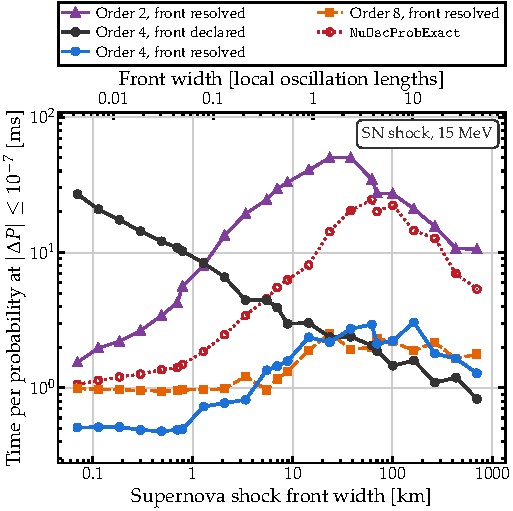
\includegraphics[width=\columnwidth]{shock_cost.pdf}
 \caption{\label{fig:shock_cost}\textbf{Cost of crossing a supernova shock front.} Time to compute one probability to within $\lvert \Delta P \rvert \leq 10^{-7}$ on the supernova ray of \figu{shock}, against the width of its two fronts. The upper axis divides each width by the oscillation length at the front, about 16~km (Sec.~\ref{sec:shock}). For each width and each curve, we find the smallest slab count that reaches the target and time that setting. Each time is the best of three timed blocks after a discarded warm-up, divided by 61, the number of baselines one call returns, so it gives the cost of one probability within a scan. \textit{Front declared} passes the two edges of each front through {\tt t\_breakpoints}; \textit{front resolved} also marks points inside each front. See notebook \#28 and Sec.~\ref{sec:shock_comparison} for details.}
\end{figure}
%%%%%%%%%%%%%%%%%%%%%%%%%%%%%%%%%%%%%%%%%%%%%%%%%%%%%

Figure~\ref{fig:shock_cost} shows the time to compute one probability to within $\lvert \Delta P \rvert \leq 10^{-7}$ on the supernova ray of \figu{shock}, for fronts from 0.07 to 701~km wide, using \magnus\ and {\tt NuOscProbExact}. \magnus\ is called as
\begin{verbatim}
 P = oscprob.osc_prob_matter_std_potential(
    3, ne_shock(width), E, Ls, osc, L0=L0,
    density_is_of_number_of_electrons=True,
    t_breakpoints=front_edges(width, n, resolve),
    magnus_exp_order=order, cumulative=True,
    n_slabs=n, max_n_slabs=n,
    rtol=1.0e-12, atol=1.0e-14)
\end{verbatim}
with {\tt E} the neutrino energy, 15~MeV, and {\tt Ls} an array of 61 baselines along the ray, so that one call returns that many probabilities. The function {\tt ne\_shock(width)} gives the electron density along the ray. Beyond the forward shock, the star is undisturbed and the density falls as $r^{-2.4}$. The shock compresses it about tenfold at the front. Behind the front, a rarefaction lowers it to about a fifth of the undisturbed value by the contact discontinuity, across which it rises again by a factor of 2.5. The two fronts sit at 30\,323 and 12\,348~km; {\tt width} sets the distance over which each makes its transition. The function {\tt front\_edges} returns the two edges of each front, plus points inside them when {\tt resolve} is {\tt True}; {\tt t\_breakpoints} places a slab edge at each of those positions. Setting {\tt n\_slabs} and {\tt max\_n\_slabs} to the same value fixes the slab count at exactly {\tt n}. We dial slab count rather than tolerance because on this ray a tighter tolerance does not reliably give a better answer: the error comes from the slab spanning the front, which refining the rest of the ray does not change. For each width and each curve, we take the smallest {\tt n} that reaches the target and time the call at that value.

The front width sets the cost, differently for each code. \magnus\ becomes expensive when the front is narrower than its slabs and only two edges are declared: a single slab then spans the whole front. Marking points inside the front---\textit{resolving} it---removes that cost. {\tt NuOscProbExact}, and \magnus\ at order 2, which works the same way, become expensive at intermediate widths. There, the density changes too fast to be treated as constant within a slab, but too slowly to be treated as one jump.

\smallskip

\textit{Declaring a front vs.~resolving it.---}Declaring the two edges of a front with {\tt t\_breakpoints} places a slab edge on each, bracketing the front at every level of the refinement. Elsewhere, the slabs are uniform, with a spacing equal to the length of the ray divided by the slab count. On the 70\,000-km ray, that spacing stays wider than a 0.07-km front until the slab count approaches a million. Until then, the front is spanned by a single slab between the two declared edges. Raising the slab count narrows every other slab on the ray, but not that one, and that one slab dominates the error, since the Hamiltonian changes sharply only there. At Magnus order 4, the error $\lvert \Delta P \rvert$ stays between $2.5 \cdot 10^{-6}$ and $4 \cdot 10^{-6}$ from 10\,000 to 250\,000 slabs. (Figure~\ref{fig:shock_cost} does not show this, since it plots cost rather than error against slab count.) Resolving the front, by also marking points inside it, removes that plateau: eight slabs per front are enough to reach $\lvert \Delta P \rvert \leq 10^{-7}$. \figu{shock_cost} shows both cases, as the \textit{front declared} and \textit{front resolved} curves.

Resolving the front can reduce the cost substantially. At 0.07~km and Magnus order 4---the default---reaching $\lvert \Delta P \rvert \leq 10^{-7}$ takes 27~ms per probability with the fronts declared, and 0.5~ms with them resolved. The saving depends on how many slabs the uniform grid would place inside the front by itself. Where it would place fewer than one, resolving saves a factor of tens. At a 9-km front, where it places about nine, resolving saves a factor under two. The declared and resolved curves at order 4 cross near 30~km. Beyond that, resolving only adds work: at 700~km, where the grid already places about 190 slabs inside each front, the extra edges add about half to the cost. \textit{So the user should resolve a front only when the uniform grid would not reach inside it.}

\smallskip

\textit{Why a front of middling width is expensive.---}The costs of \magnus\ at order 2 and of {\tt NuOscProbExact} rise as the front widens, peak between about 20 and 60~km, then fall; \magnus\ at orders 4 and above shows no such peak. The reason lies in how a neutrino crosses a front. The states that propagate unchanged in matter are combinations of flavor states set by the local density, so a front rotates them. Across a wide front, the rotation is slow compared with an oscillation, and the neutrino follows it: the crossing is adiabatic, and the front needs no resolving. Across a thin front, the neutrino has no time to follow and crosses unchanged: the crossing is sudden, and a declared breakpoint represents it exactly. A front of middling width is in neither limit, so the slabs must resolve it.

Two measures locate this range. The first is the front width in oscillation lengths at the front, about 16~km (Sec.~\ref{sec:shock}), shown on the upper axis of \figu{shock_cost}: the cost peaks between about 1.5 and 4. The second needs no run: the non-adiabaticity $\gamma_{jk}$ of \equ{hf}, evaluated across the front and maximized over pairs of instantaneous eigenstates. It falls from about 730 at the thinnest front to about 0.08 at the widest, and crosses 1 between 38 and 62~km, where the measured costs peak.

Higher Magnus orders avoid the peak because of their commutators. A constant-density slab, as in {\tt NuOscProbExact} or \magnus\ at order 2, holds the Hamiltonian fixed across its length. At a middling front, the propagating states rotate inside each slab, so every slab is slightly wrong, and the only remedy is to narrow them: hence the peak. At orders 4 and above, \magnus\ samples $\mathbb{A}$ at several points inside each slab and keeps the commutators between those samples. These capture the change of the Hamiltonian within a slab, so fewer, wider slabs suffice and the run time falls. Each higher order keeps more samples and flattens the curve further.

%%%%%%%%%%%%%%%%%%%%%%%%%%%%%%%%%%%%%%%%%%%%%%%%%%%%%

\subsection{Accuracy and speed: the Sun}
\label{sec:solar_comparison}

%%%%%%%%%%%%%%%%%%%%%%%%%%%%%%%%%%%%%%%%%%%%%%%%%%%%%
\begin{figure}[t!]
 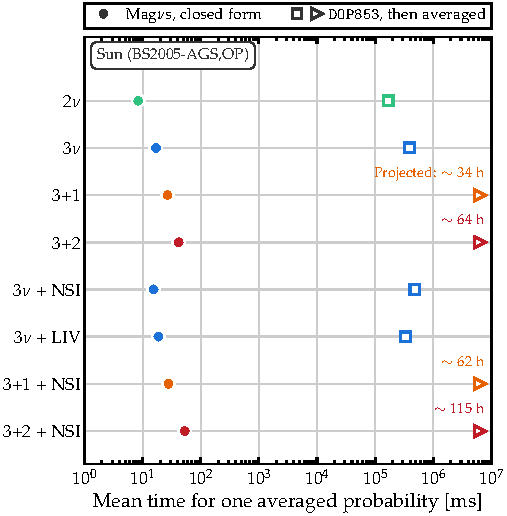
\includegraphics[width=\columnwidth]{solar_average_cost.pdf}
 \caption{\label{fig:solar_average_cost}\textbf{Cost of an averaged solar probability.} Time to compute one averaged $\nu_e$ survival probability through the Sun at 5~MeV, for eight configurations. The density is the tabulated BS2005-AGS,OP model, interpolated in its logarithm, not the exponential fit that {\tt osc\_prob\_*\_sun} uses by default; the two are different problems with different costs. The evolution is adiabatic throughout and every pair of eigenstates has decohered on arrival, so the level-crossing matrix is the identity and \equ{averaged_varying} needs only one eigendecomposition at production and one at detection, exact to about $10^{-15}$. We compare against the same average obtained by integration: a {\tt DOP853} solve at ${\tt rtol} = 10^{-8}$, the loosest tolerance that still reproduces \magnus's result, followed by the mean of the oscillating probability over the last 1\% of the ray. The quoted time covers both steps. The active-sterile mixing parameters are $\sin^2\theta_{14} = \sin^2\theta_{24} = 0.1$ and $\Delta m^2_{41} = 1$~eV$^2$ for 3+1, and in addition $\sin^2\theta_{15} = \sin^2\theta_{25} = 0.05$ and $\Delta m^2_{51} = 2$~eV$^2$ for 3+2. For these, the integration is projected from a measured segment of the ray, since eV-scale splittings put $10^{8}$ oscillations along it and resolving them would take too long. See notebook \#28 and Sec.~\ref{sec:solar_comparison} for details.}
\end{figure}
%%%%%%%%%%%%%%%%%%%%%%%%%%%%%%%%%%%%%%%%%%%%%%%%%%%%%

Figure~\ref{fig:solar_average_cost} shows the cost of the averaged survival probability, \equ{averaged_varying}, of a 5-MeV solar neutrino for two to five flavors, with and without non-standard interactions and Lorentz violation. \magnus\ is called as
\begin{verbatim}
 P = oscprob.osc_prob_3nu_sun(E,
    solarmodels.table_edge('BS05-AGS-OP'), 0.0,
    density_profile='BS05-AGS-OP',
    average=True, nu_i=gd.NUE, nu_f=gd.NUE)
\end{verbatim}
for the standard three-flavor case, and similarly for the others. The option {\tt density\_profile} selects the tabulated BS2005-AGS,OP solar model, and {\tt solarmodels.table\_edge} returns the distance to its last tabulated radius, where the path ends ($0.983\,R_\odot$). \magnus\ is four or more orders of magnitude faster than the {\tt DOP853} integration.

The two approaches differ in what they compute:
\begin{itemize}
\item \textit{{\tt DOP853}} integrates the evolution along the whole path, resolving some $10^{5}$ oscillation cycles, and only then averages them away.
\item \textit{\magnus} computes no oscillation at all. It diagonalizes the Hamiltonian at production and at detection, then evaluates \equ{averaged_varying} from the two sets of eigenvectors. This two-endpoint formula holds only if the neutrino stays in the same instantaneous eigenstate all the way out, so \magnus\ first searches the path for non-adiabatic crossings (Sec.~\ref{sec:hybrid}); on this profile it finds none.
\end{itemize}
The search takes about four fifths of \magnus's time; the two diagonalizations, a fraction of a percent. Both depend on the size of the Hamiltonian, set by the number of flavors, and hardly on its entries. The cost rises from 5~ms at two flavors to 16~ms at five, while non-standard interactions and Lorentz violation, which change only the entries, add little.

%%%%%%%%%%%%%%%%%%%%%%%%%%%%%%%%%%%%%%%%%%%%%%%%%%%%%
%%%%%%%%%%%%%%%%%%%%%%%%%%%%%%%%%%%%%%%%%%%%%%%%%%%%%

\section{Comparison to other codes}
\label{sec:comparison}

%%%%%%%%%%%%%%%%%%%%%%%%%%%%%%%%%%%%%%%%%%%%%%%%%%%%%

\subsection{Relation to other oscillation codes}
\label{sec:relation}

We compare the performance of \magnus\ against several mature oscillation codes:
\begin{itemize}
\item {\tt GLoBES}\ \cite{GLoBES, Huber:2007ji} is an experiment-simulation framework in which probabilities are one layer inside a package built for fluxes, cross-sections and detector response.
\item {\tt Prob3++}\ \cite{Prob3pp} evaluates the analytic three-flavor probability in matter\ \cite{Barger:1980tf} and is long established in atmospheric analyses.
\item {\tt nuCraft}\ \cite{nuCraft} integrates numerically along a chord through the Earth.
\item {\tt NuFast-LBL}\ \cite{Denton:2024pzc} and {\tt NuFast-Earth}\ \cite{Denton:2025oxf} are fast specializations of the three-flavor case.
\item {\tt NuOscProbExact}\ \cite{NuOscProbExact, Bustamante:2019ggq} evaluates closed-form SU($n$) expansions of the evolution operator for an arbitrary Hermitian Hamiltonian at two, three, and four flavors, and composes them across slabs of constant density.
\item {\tt nuSQuIDS}\ \cite{Delgado:2014kpa, Arguelles:2021twb, NuSQuIDS} is the most general: it propagates a density matrix rather than a state, which admits interactions, attenuation and open-system terms that no closed form reaches, at the cost of solving a differential equation.
\end{itemize}
Structurally, \magnus\ sits between {\tt NuOscProbExact} and {\tt nuSQuIDS}: it composes slab exponentials as the first does, while resolving the variation of the Hamiltonian within each slab as the second would, though via different means.

%%%%%%%%%%%%%%%%%%%%%%%%%%%%%%%%%%%%%%%%%%%%%%%%%%%%%

\subsection{Speed-accuracy comparison}
\label{sec:prem_planes}

%%%%%%%%%%%%%%%%%%%%%%%%%%%%%%%%%%%%%%%%%%%%%%%%%%%%%
\begin{figure*}[t!]
 \centering
 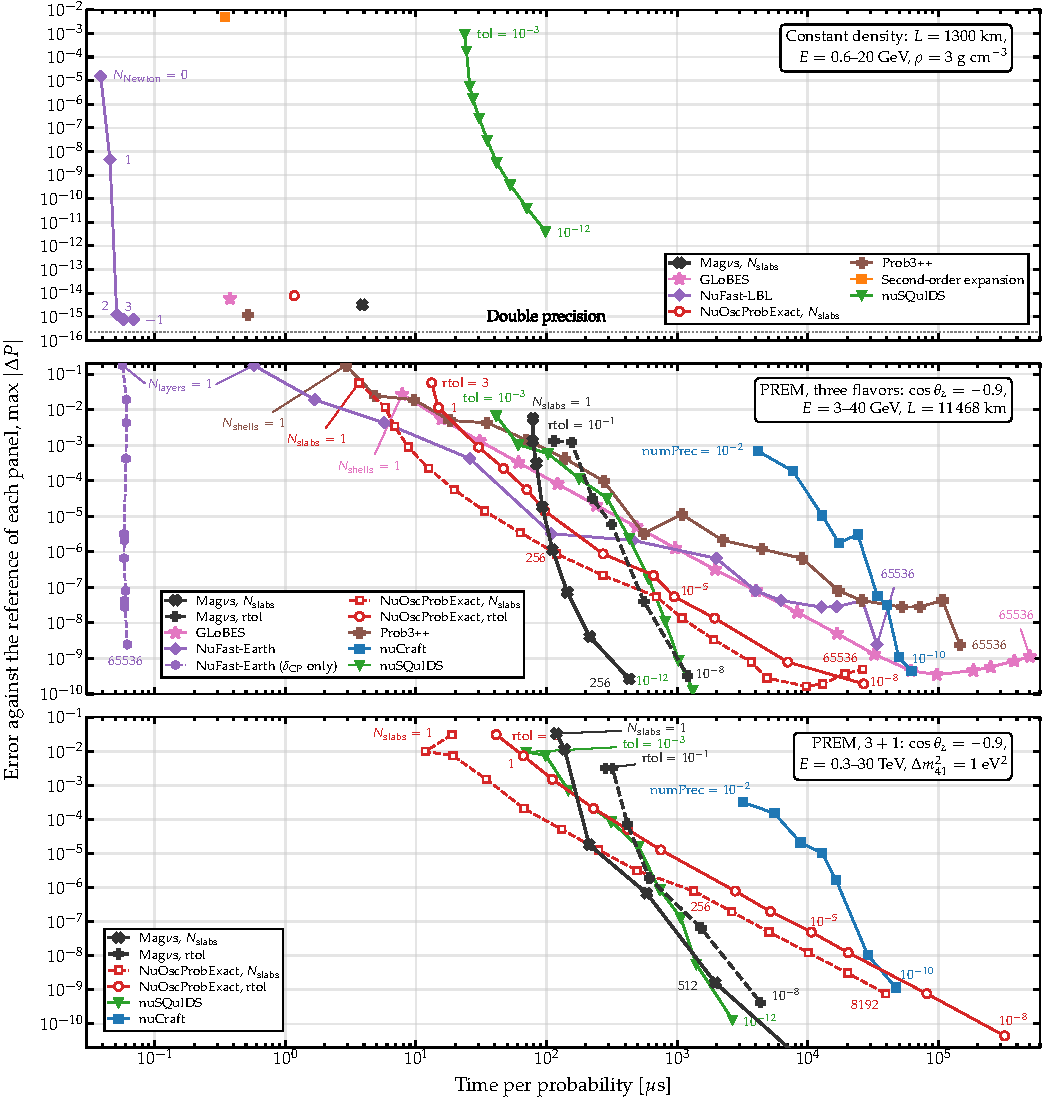
\includegraphics[width=\textwidth]{speed_accuracy_combined.pdf}
 \caption{\label{fig:prem_plane}Error in the probability calculation against each code's own reference, plotted against time per probability, for eight codes on three setups: constant density ({\it top}); a core-crossing PREM Earth chord at $\cos\theta_z = -0.9$, baseline $11\,468$~km, at three flavors ({\it middle}); the same chord with one sterile state ({\it bottom}). \magnus\ and {\tt NuOscProbExact} appear twice in the Earth panels because each turns two dials, a slab count and a tolerance; {\tt NuFast-Earth} appears twice because its cost depends on which oscillation parameter the scan varies. See Sec.~\ref{sec:prem_planes} for details.}
\end{figure*}
%%%%%%%%%%%%%%%%%%%%%%%%%%%%%%%%%%%%%%%%%%%%%%%%%%%%%

Figure~\ref{fig:prem_plane} compares the eight codes on three setups: constant density at three flavors, a core-crossing Earth chord at three flavors, and the same chord at 3+1 flavors. Every point is one setting of one code, ranked by the time it takes per probability and the error it returns. Each code is scored against a 50-digit reference built that adopts the code's own constants and conventions--chiefly, the nucleon mass that fixes $V_{\rm CC}$. Thus, two codes can reach $10^{-14}$ on the y-axis of \figu{prem_plane} and still disagree with each other at $10^{-4}$.

Every code evaluates the probability at energies over a fixed logarithmic grid; the error plotted in \figu{prem_plane} is the largest deviation found over that grid. The constant-density panel uses sixty energies from $0.6$ to $20$~GeV; the Earth chord at three flavors, twelve from $3$ to $40$~GeV; the same chord at $3+1$, twelve from $300$ to $30\,000$~GeV, three decades higher because an eV-scale $\Delta m^2_{41}$ puts its resonance there. The mixing parameters are the same for every code: $\delta_{\rm CP} = 217^\circ$, $\Delta m^2_{21} = 7.39 \cdot 10^{-5}$~eV$^2$, $\Delta m^2_{31} = 2.525 \cdot 10^{-3}$~eV$^2$. For the timing, $\delta_{\rm CP}$ is stepped 25 times, with the whole energy grid evaluated at each step.

\smallskip

\textit{Constant density.---}At constant density (\figu{prem_plane}, top panel), the evolution operator is one exponential carrying no discretization at all. Most of the codes land within a factor of a few of double-precision round-off, near $10^{-15}$, and separate only in cost: from $0.04$~$\mu$s for {\tt NuFast-LBL} to about $100$~$\mu$s for {\tt nuSQuIDS}, three orders of magnitude for the same answer. \magnus\ sits at $3 \cdot 10^{-15}$ and $3.9$~$\mu$s. For {\tt GLoBES}, {\tt Prob3++} and {\tt NuOscProbExact}, their refinement dials subdivide a profile that does not vary, so they changes their cost a little and their error not at all; their points lie along a horizontal line.

The second-order expansion has no dial either: it is the analytic formula for $P_{\nu_\mu \to \nu_e}$ to second order in $\alpha = \Delta m^2_{21}/\Delta m^2_{31}$ and $s_{13}$\ \cite{Cervera:2000kp, Freund:2001pn}. It is the second-cheapest point on the panel, but also the least accurate. That error is a truncation of the series rather than a discretization, so no setting moves it.

Only {\tt NuFast} and {\tt nuSQuIDS} trace a curve, the former over the number of Newton steps and the latter over its solver tolerance. The time spread between the two reflects how narrowly each code is specialized to the constant-density problem. {\tt NuFast-LBL} evaluates a three-flavor closed form in constant-density matter as scalar arithmetic, refining its eigenvalues by Newton iteration, which is why it is the cheapest point here. {\tt nuSQuIDS} sits at the other end because it integrates a density matrix through a problem whose answer is a single exponential, paying for generality that constant density does not need.

\smallskip

\textit{Earth chord, three flavors.---}Through the Earth (\figu{prem_plane}, middle panel) the density changes along the chord, so each code builds its own approximation of the profile, and the figure measures how finely it resolves it.

We show two \magnus\ curves: one varying its slab count, {\tt N\_slabs}, and one varying its tolerance, {\tt rtol}. Given {\tt N\_slabs}, \magnus\ evaluates once at that count: from 4 to 256 slabs, the error falls from $1.3 \cdot 10^{-3}$ to $2.6 \cdot 10^{-10}$, while the cost rises only from about 80 to 430~$\mu$s. Below about thirty slabs, the time is primarily due to overhead; beyond that, the number of slabs drive the time, which doubles with their number. Given {\tt rtol} instead, \magnus\ climbs the refinement ladder and pays for every level it evaluates and discards: ${\tt rtol} = 10^{-8}$ returns $3.2 \cdot 10^{-10}$--the same accuracy as for 256 slabs---for a longer run time of about 1200~$\mu$s. Thus, at matched accuracy, the ladder costs about three times the direct call; this is the price of the convergence evidence it returns with the answer.

The other codes reach comparable accuracy at very different cost. To achieve an accuracy of about $3 \cdot 10^{-10}$, {\tt nuSQuIDS} needs 1.3~ms, {\tt NuOscProbExact} 26~ms, {\tt nuCraft} 62~ms, and {\tt GLoBES} 0.5~s, against 0.43~ms for \magnus. The three-flavor specializations are the cheapest codes when little accuracy is asked of them and the most expensive when much is. Their only dial is the number of layers they cut the Earth into, with the cost growing in proportion to that number. \Eg, {\tt NuFast-Earth} starts at 0.6~$\mu$s with an error of 0.18, and reaches $2.5 \cdot 10^{-9}$ only at 34~ms. {\tt nuCraft} runs the other way, starting already at $7 \cdot 10^{-4}$ and never costing less than 4~ms. The difference is where the integrand lives: {\tt nuCraft} hands {\tt SciPy}'s {\tt zvode} function---an ordinary-differential-equation solver--- a right-hand side and Jacobian, which are called once per internal step and rebuild the Hamiltonian each time, so its dial buys accuracy by adding steps that are expensive one by one.

{\tt NuOscProbExact} and \magnus\ cross near an error of $10^{-6}$. Because of its closed-form probabilities, {\tt NuOscProbExact} starts twenty times cheaper: its coarsest setting costs about 4~$\mu$s per probability, against 80~$\mu$s for \magnus. What separates them is the work inside one slab. The closed form samples the density at the slab's midpoint and holds it constant across the slab, which is the second-order Magnus step of Sec.~\ref{sec:order_is_the_slab_product}, so its error falls as the square of the slab width. \magnus\ at order 4 samples the Hamiltonian at two Gauss-Legendre points inside the slab and computes their commutator, so it resolves how the density varies across the slab, and its error falls as the fourth power. The PREM density varies continuously inside every shell, so there is variation for that commutator to resolve. Each doubling of the slab count therefore divides the closed form's error by $2^2$ and \magnus's by $2^4$, which is why the \magnus\ curves eventually cross the {\tt NuOscProbExact} curves, becoming the faster option. 

Figure~\ref{fig:prem_plane} contains two {\tt NuFast-Earth} curves because it is the only code here whose cost depends on which oscillation parameter a scan moves. Every timed scan in the figure varies $\delta_{\rm CP}$; substituting $\Delta m^2_{31}$ changes the cost of the other codes by at most two per cent. {\tt NuFast-Earth} reuses its layer solve when varying $\delta_{\rm CP}$, so its cost per probability stays near $0.06~\mu$s at every layer count in the sweep. The second {\tt NuFast-Earth} curve is the same sweep of $\Delta m^2_{31}$, a parameter the cache does not cover. Its cost climbs with the layer count and falls inside the band the rest of the panel occupies. 

\smallskip

\textit{Earth chord, $3+1$ flavors.---}The bottom panel of \figu{prem_plane} adds a sterile state, which three of the codes cannot handle: {\tt NuFast-Earth}, {\tt GLoBES} (without extensions), and {\tt Prob3++}. Of the remaining codes, {\tt nuSQuIDS} is the one closer to \magnus.

The crossing between {\tt NuOscProbExact} and \magnus\ survives, moved up an order of magnitude in error to about $10^{-5}$. Each code converges at the rate it did at three flavors: doubling the slab count still divides {\tt NuOscProbExact}'s error by $2^2$ and \magnus's by $2^4$. The head start is what changes: a slab costs {\tt NuOscProbExact} 8 times what it cost at three flavors, against under 3 for \magnus. The reason is the cost of the eigenvalues in {\tt NuOscProbExact}. At three flavors, they come from algebra~\cite{Bustamante:2019ggq}, which is what makes the closed-form probabilities fast. At $3+1$, {\tt NuOscProbExact} must use a more expensive eigensolver instead. Nevertheless, it remains the fastest code at the coarsest accuracies of $10^{-3}$--$10^{-5}$ because it has little overhead.

%%%%%%%%%%%%%%%%%%%%%%%%%%%%%%%%%%%%%%%%%%%%%%%%%%%%%

\subsection{When to use \magnus}
\label{sec:when_magnus}

\magnus\ is the code to reach for when the profile, the accuracy, the flavor count, or the Hamiltonian takes a problem outside what a composition of constant-density slabs does well.

\begin{itemize}
\item \textbf{The density varies continuously and fast against the oscillation length.} A composition of constant-density slabs needs some $10^4$ steps per resonance crossing in the Sun, where \magnus\ integrates across the slab instead.
\item \textbf{The profile has structure at a known place.} A shock front, a layer boundary, or a kink is passed as {\tt t\_breakpoints}, which puts a slab edge on it at every refinement level (Sec.~\ref{sec:declaring_edges}).
\item \textbf{The problem has more than three flavors.} At $3+1$ {\tt NuOscProbExact} must find its eigenvalues numerically, at 8 times the cost per slab; past four flavors the SU($n$) closed forms stop altogether.
\item \textbf{The Hamiltonian has no closed form of its own.} Nothing in \magnus\ assumes a form for $\mathbb{H}(l)$ beyond Hermiticity, so a non-standard interaction, a Lorentz-violating background, or a completely novel Hamiltonian is supplied transparently as a matrix and needs no change to the solver.
\item \textbf{The observable is an average.} Phase-averaged probabilities and flavor composition are returned directly instead of reconstructed from a scan (Sec.~\ref{sec:averaged}).
\item \textbf{The accuracy required lies below where a slab composition floors.} On a core-crossing PREM chord, {\tt NuOscProbExact} stops near $2 \cdot 10^{-10}$, while \magnus\ reaches further (Sec.~\ref{sec:prem_planes}). (Both sit far below the per-cent level at which probabilities in data analysis, though.)
\end{itemize}

Elsewhere, another code may be cheaper. On constant density, closed-form and specialized codes reach double precision; the three-flavor specializations {\tt NuFast-LBL} and {\tt NuFast-Earth} do so for about $0.07$~$\mu$s per probability, some sixty times faster than \magnus. On a piecewise-constant profile resolved to no better than about $10^{-6}$, {\tt NuOscProbExact} is the cheapest of them; a three-flavor fit that moves only $\delta_{\rm CP}$ is cheaper still with {\tt NuFast-Earth}. Decay, decoherence, and collective effects lie outside every unitary solver here; they need the density matrix that {\tt nuSQuIDS} propagates (Sec.~\ref{sec:limitations}).

%%%%%%%%%%%%%%%%%%%%%%%%%%%%%%%%%%%%%%%%%%%%%%%%%%%%%
%%%%%%%%%%%%%%%%%%%%%%%%%%%%%%%%%%%%%%%%%%%%%%%%%%%%%

\section{Conclusions}
\label{sec:conclusions}

We have presented \magnus\ \cite{Magnus}, a general-purpose code for computing neutrino oscillation probabilities, in the Standard Model and beyond. It accepts any Hamiltonian, position-dependent or not, at any number of flavors, through any density profile. The restriction is that the Hamiltonian be Hermitian. \magnus\ is designed to take numerical work off the user: given a Hamiltonian, it chooses the method, sets the resolution needed to meet the requested tolerance, and returns the probabilities, so that the user need not write or validate a solver of their own. \magnus\ is robust, flexible, and fast even when the neutrino oscillates many times along its path.

At the core of \magnus\ is the Magnus expansion, which replaces the solution of the differential equation for the evolution operator by integrals of the Hamiltonian and its commutators along the neutrino trajectory. \magnus\ places no restriction on the size of the Hamiltonian, on what it contains, or on why it varies along the trajectory. A changing matter profile, a Lorentz-violating background, and active-sterile mixing are merely different Hamiltonians; the method that computes the probabilities is the same.

To apply the expansion, \magnus\ cuts the trajectory into slabs, computes the evolution operator across each, and composes them time-ordered, determining the number of slabs needed to meet the requested tolerance. The evolution is unitary at any number of slabs and any order of the expansion, so the probabilities always sum to one over all flavors. To boost accuracy, slab edges can be pinned to the discontinuities of a profile, as inside the Earth or across a supernova shock front.

Where a request can be answered exactly or more cheaply than with the expansion, \magnus\ does so automatically: with a single exponential when the Hamiltonian does not vary, by following the slowly changing eigenstates of a smooth profile, or by computing many energies or baselines together. Besides oscillating probabilities, \magnus\ returns averaged ones, which describe, \eg, solar and high-energy astrophysical neutrinos. Against existing oscillation codes, \magnus\ matches their accuracy, and where high accuracy is needed on a varying density profile, it is the fastest of those we compared; at coarse accuracy or constant density, simpler codes are cheaper (Sec.~\ref{sec:comparison}).

We have shown \magnus\ at work on examples across the field: layered matter, core-crossing Earth chords, the Sun, a supernova shock front, the flavor composition of astrophysical neutrinos, geoneutrinos, a jet inside a collapsing star, turbulent matter, and several scenarios of new physics, including a Hamiltonian supplied by the user. Each is a variation on one call, with the Hamiltonian, the profile, or the observable changed. A command-line tool computes the same probabilities without writing any Python code. The repository~\cite{Magnus} holds 29 executable notebooks, from first steps to advanced uses; one of them reproduces every figure in this paper.

Two classes of problem lie beyond \magnus. First, decoherence, coupling to a bath, and decay to invisible states are not unitary and need a density-matrix treatment. Second, collective oscillations in a dense neutrino gas are nonlinear: self-interaction makes the Hamiltonian change as they evolve.

\magnus\ is available from the Python Package Index with {\tt pip install magnuspy} and from its repository\ \cite{Magnus}.
%%%%%%%%%%%%%%%%%%%%%%%%%%%%%%%%%%%%%%%%%%%%%%%%%%%%%
%%%%%%%%%%%%%%%%%%%%%%%%%%%%%%%%%%%%%%%%%%%%%%%%%%%%%

\section*{Declaration of generative AI and AI-assisted technologies in the manuscript preparation process}

During the preparation of this work, the author used Claude  as research assistance for code development, numerical auditing, workflow documentation, repository maintenance, and editorial revision. All scientific judgments, validation decisions, and responsibility for the manuscript remain with the author

%%%%%%%%%%%%%%%%%%%%%%%%%%%%%%%%%%%%%%%%%%%%%%%%%%%%%
%%%%%%%%%%%%%%%%%%%%%%%%%%%%%%%%%%%%%%%%%%%%%%%%%%%%%

\section*{Acknowledgments}

MB is supported by the {\sc Villum Fonden} project no.~29388.

%%%%%%%%%%%%%%%%%%%%%%%%%%%%%%%%%%%%%%%%%%%%%%%%%%%%%
%%%%%%%%%%%%%%%%%%%%%%%%%%%%%%%%%%%%%%%%%%%%%%%%%%%%%

\bibliographystyle{elsarticle-num}
\bibliography{refs.bib}

%%%%%%%%%%%%%%%%%%%%%%%%%%%%%%%%%%%%%%%%%%%%%%%%%%%%%
%%%%%%%%%%%%%%%%%%%%%%%%%%%%%%%%%%%%%%%%%%%%%%%%%%%%%

\appendix

\renewcommand{\thefigure}{\Alph{section}.\arabic{figure}}
\renewcommand{\thetable}{\Alph{section}.\arabic{table}}
\newcommand{\appresetfloats}{\setcounter{figure}{0}\setcounter{table}{0}}

%%%%%%%%%%%%%%%%%%%%%%%%%%%%%%%%%%%%%%%%%%%%%%%%%%%%%

\section{Magnus expansion at any order}
\label{app:terms}
\appresetfloats

Section \ref{sec:expansion} gave the definition of the Magnus expansion via recursion.  This appendix gives its structure, which is what makes a relatively succinct implementation. The maximum expansion order in \magnus\ is set to {\tt MAGNUS\_EXP\_ORDER\_MAX=10}. Orders nine and ten of the  expansion need either Simpson's rule or the trapezoidal rule to integrate, since the Gauss-Legendre collocation of \equ{gl} stop at order eight ({\tt MAGNUS\_EXP\_ORDER\_MAX\_GL=8}).

\subsection{Computing Magnus terms}

Unrolling the recursion equation, \equ{recursion}, every term of $\Omega_n$ is a right-nested chain
\begin{equation}
 \label{equ:nested}
 \left[\Omega_{m_1}, \left[\Omega_{m_2}, \ldots
 \left[\Omega_{m_j}, \mathbb{A}\right] \ldots \right]\right] \;,
 \quad
 \sum_{i=1}^{j} m_i = n-1 \;,
\end{equation}
carrying the coefficient $B_j/j!$. Therefore, the terms of the $j$-th group are indexed by the compositions of $n-1$ into $j$ positive parts, of which there are $\binom{n-2}{j-1}$. Since $B_j$ vanishes for odd $j \geq 3$, the number of terms in $\Omega_n$ is
\begin{equation}
 \label{equ:term_count}
 \#\,\Omega_n = \sum_{j\,:\,B_j \neq 0} \binom{n-2}{j-1} \;.
\end{equation}
The surviving coefficients, of which an implementation to order 10 needs exactly these five, are
\begin{eqnarray}
 \label{equ:bernoulli}
 && \frac{B_1}{1!} = -\frac{1}{2} , \;
 \frac{B_2}{2!} = \frac{1}{12} , \;
 \frac{B_4}{4!} = -\frac{1}{720} , \; \nonumber \\
 && \frac{B_6}{6!} = \frac{1}{30240} , \;
 \frac{B_8}{8!} = -\frac{1}{1\,209\,600} \;.
\end{eqnarray}
A term with $j$ nested commutators requires $j \leq n-1$, so $B_8$ first appears at order 9 (and $B_{10}$ not until order 11). Equation (\ref{equ:term_count}) gives $1, 1, 2, 3, 5, 9, 17, 33, 65, 129$ terms at orders 1 to 10, the count doubling from order 5 onward, which is why \magnus\ implements an order ceiling: the terms remain easy to generate far beyond it, but the work per slab grows with their number.

The module {\tt magnus.expansionterms} evaluates all of this in exact rational arithmetic at any order, with coefficients returned as fractions so that they can be compared exactly, not at a tolerance. This module shares no code with the numerical core of \magnus: the test suite regenerates the hard-coded group factors and compares them against the derived ones, and separately evaluates the generated terms numerically on a sampled $\mathbb{A}(l)$ and compares them order by order against what the core produces internally. Agreement is at machine precision for every order from one to ten, covering the hard-coded low orders and the generated high ones.

\subsection{Why the collocation orders are even}

Two facts fix the leading power of $h$ in each $\Omega_k$. The first is a parity: traversing a slab backwards inverts the evolution, so $\Omega$ changes sign; it does so term by term, since reversal cannot change how many factors of $\mathbb{A}$ a term carries. Measured from the slab midpoint, traversing backwards replaces $h$ by $-h$, so each $\Omega_k$ carries only odd powers of $h$. The second is a cost: above $\Omega_1$, every term is a nested commutator of $\mathbb{A}$ with itself at different positions, which vanishes for constant $\mathbb{A}$. The second fact is the effect of the commutators. Above $\Omega_1$, every term holds at least one commutator of $\mathbb{A}$ at two points of the slab. That commutator vanishes for constant $\mathbb{A}$, so its magnitude follows the variation of $\mathbb{A}$ across the slab, itself $\mathcal{O}(h)$ for smooth $\mathbb{A}$. Each term above $\Omega_1$ thus gains one power of $h$ beyond its $k$ integrations, placing $\Omega_k$ at $h^{k+1}$.

The two facts meet at odd $k$, where $h^{k+1}$ is an even power. The parity forbids it, so the term enters at $h^{k+2}$ instead. Hence $\Omega_1$ enters at $h$ and $\Omega_2$ at $h^3$; from $\Omega_3$ upward the terms pair off, $\Omega_{2j-1}$ and $\Omega_{2j}$ both entering at $h^{2j+1}$ for $j \geq 2$. Both statements of Sec.~\ref{sec:quadrature} follow. A scheme of order $p$ carries a local error $\mathcal{O}(h^{p+1})$, so it retains every term entering below that power: $\Omega_1$ alone at $p = 2$, $\Omega_1$ through $\Omega_{p-2}$ for $p \geq 4$. The leading term it drops sets its error on one slab, at an odd power of $h$. A trajectory of $N$ slabs accumulates those errors, so $h^q$ on each leaves $h^{q-1}$ over the whole path. Odd $q$ makes $q-1$ even: the schemes exist at even order only.

%%%%%%%%%%%%%%%%%%%%%%%%%%%%%%%%%%%%%%%%%%%%%%%%%%%%%
%%%%%%%%%%%%%%%%%%%%%%%%%%%%%%%%%%%%%%%%%%%%%%%%%%%%%

\section{Predefined oscillation-parameter sets}
\label{app:params}
\appresetfloats

Section \ref{sec:params} showed how to select a set of standard oscillation parameters by name. \tabl{params} lists  the fifty-two sets \magnus\ recognizes, one for each NuFIT release\ \cite{Esteban:2024eli} and mass ordering.

%%%%%%%%%%%%%%%%%%%%%%%%%%%%%%%%%%%%%%%%%%%%%%%%%%%%%
{\def\arraystretch{1.08}
\begin{table*}[t!]
{\small
\begin{tabular}{@{}p{2.1cm}p{1.0cm}p{2.6cm}p{10.0cm}@{}}
 Release & Year & Fit & How to select it \\
 \hline
 NuFIT 1.0 & 2012 & free fluxes & {\tt OSC\_PARAMS\_NU\_FIT\_1\_0} \\
  &  & Huber fluxes & {\tt category='huber\_fluxes\_no\_rsbl'} \\
 NuFIT 1.1 & 2013 & free fluxes & {\tt OSC\_PARAMS\_NU\_FIT\_1\_1} \\
  &  & Huber fluxes & {\tt category='huber\_fluxes\_no\_rsbl'} \\
 NuFIT 1.2 & 2013 & free fluxes & {\tt OSC\_PARAMS\_NU\_FIT\_1\_2} \\
  &  & Huber fluxes & {\tt category='huber\_fluxes\_no\_rsbl'} \\
 NuFIT 1.3 & 2014 & free fluxes & {\tt OSC\_PARAMS\_NU\_FIT\_1\_3} \\
  &  & Huber fluxes & {\tt category='huber\_fluxes\_no\_rsbl'} \\
 NuFIT 2.0 & 2014 & single fit & {\tt OSC\_PARAMS\_NU\_FIT\_2\_0} \\
 NuFIT 2.1 & 2016 & LEM analysis & {\tt OSC\_PARAMS\_NU\_FIT\_2\_1} \\
  &  & LID analysis & {\tt category='LID'} \\
 NuFIT 2.2 & 2016 & single fit & {\tt OSC\_PARAMS\_NU\_FIT\_2\_2} \\
 NuFIT 3.0 & 2016 & single fit & {\tt OSC\_PARAMS\_NU\_FIT\_3\_0} \\
 NuFIT 3.1 & 2017 & single fit & {\tt OSC\_PARAMS\_NU\_FIT\_3\_1} \\
 NuFIT 3.2 & 2018 & single fit & {\tt OSC\_PARAMS\_NU\_FIT\_3\_2} \\
 NuFIT 4.0 & 2018 & with SK & {\tt OSC\_PARAMS\_NU\_FIT\_4\_0\_SK} \\
  &  & without SK & {\tt OSC\_PARAMS\_NU\_FIT\_4\_0\_NOSK} \\
 NuFIT 4.1 & 2019 & with SK & {\tt OSC\_PARAMS\_NU\_FIT\_4\_1\_SK} \\
  &  & without SK & {\tt OSC\_PARAMS\_NU\_FIT\_4\_1\_NOSK} \\
 NuFIT 5.0 & 2020 & with SK & {\tt OSC\_PARAMS\_NU\_FIT\_5\_0\_SK} \\
  &  & without SK & {\tt OSC\_PARAMS\_NU\_FIT\_5\_0\_NOSK} \\
 NuFIT 5.1 & 2021 & with SK & {\tt OSC\_PARAMS\_NU\_FIT\_5\_1\_SK} \\
  &  & without SK & {\tt OSC\_PARAMS\_NU\_FIT\_5\_1\_NOSK} \\
 NuFIT 5.2 & 2022 & with SK & {\tt OSC\_PARAMS\_NU\_FIT\_5\_2\_SK} \\
  &  & without SK & {\tt OSC\_PARAMS\_NU\_FIT\_5\_2\_NOSK} \\
 NuFIT 5.3 & 2024 & with SK & {\tt OSC\_PARAMS\_NU\_FIT\_5\_3\_SK} \\
  &  & without SK & {\tt OSC\_PARAMS\_NU\_FIT\_5\_3\_NOSK} \\
 NuFIT 6.0 & 2024 & with SK & {\tt OSC\_PARAMS\_NU\_FIT\_6\_0\_SK} \\
  &  & without SK & {\tt OSC\_PARAMS\_NU\_FIT\_6\_0\_NOSK} \\
 NuFIT 6.1 & 2025 & with SK & {\tt OSC\_PARAMS\_NU\_FIT\_6\_1\_SK} \\
  &  & without SK & {\tt OSC\_PARAMS\_NU\_FIT\_6\_1\_NOSK} \\
\end{tabular}}
\caption{\label{tab:params}Every set of standard oscillation parameters \magnus\ recognizes. A name in the fourth column is completed with {\tt \_NO} for normal mass ordering or {\tt \_IO} for inverted, then passed as {\tt default\_osc\_params\_set\_name} to any {\tt osc\_prob\_3nu\_*} wrapper. {\tt OSC\_PARAMS\_DEFAULT} is a further name for {\tt OSC\_PARAMS\_NU\_FIT\_6\_1\_SK\_NO}, which is what an unset parameter falls back on.Some rows give a {\tt category} instead of a name. Those variants have no constant of their own; reach them with {\tt load\_nufit\_params(version, ordering, category)}, which is also how any named set can be loaded. The third column names the secondary split each release reports: whether the Super-Kamiokande atmospheric $\chi^2$ map is folded in, whether the reactor fluxes are left free or fixed to the Huber model, and, for 2.1, which of its two analyses is taken.}
\end{table*}}
%%%%%%%%%%%%%%%%%%%%%%%%%%%%%%%%%%%%%%%%%%%%%%%%%%%%%

%%%%%%%%%%%%%%%%%%%%%%%%%%%%%%%%%%%%%%%%%%%%%%%%%%%%%
%%%%%%%%%%%%%%%%%%%%%%%%%%%%%%%%%%%%%%%%%%%%%%%%%%%%%

\section{The tutorial notebooks}
\label{app:notebooks}
\appresetfloats

The {\tt notebooks/} folder contain 29 notebooks, numbered in suggested reading order. They are the long form of several of the examples in Sec.~\ref{sec:examples}: what is a paragraph and a figure here is, in a notebook, the same calculation with the reasoning around it---why a convention is what it is, what happens at the edges of the parameter range, and what the numbers were checked against. Each is stored with its outputs, so it can be read without being run. Each ends with a pointer to its neighbors. The figures that cost hours to produce are cached in the repository as well: with {\tt MAGNUS\_PAPER\_CACHE\_ONLY} set, as continuous integration sets it, notebook \#28 redraws them from stored data rather than recomputing them, and fails rather than silently recomputing if a cache entry is missing.

The notebooks are generated: one script builds them, executes them, and refuses to finish if any came back without stored outputs. Because a notebook is documentation that claims to work, continuous integration executes them to ensure this. It does so on one interpreter, splitting the load of the 29 notebooks across four parallel shards. It keys a cache on the package source and on the notebook inputs: a notebook whose inputs have not moved is served from that cache rather than run again, to save time. Therefore, a change to the package re-executes all of the notebooks, and a change to one notebook re-executes that one alone. The unit tests run across the four supported versions of Python; the notebooks are not.

%%%%%%%%%%%%%%%%%%%%%%%%%%%%%%%%%%%%%%%%%%%%%%%%%%%%%
{\def\arraystretch{1.15}
\begin{table*}[t!]
{\small
\begin{tabular}{@{}p{0.6cm}p{4.3cm}p{9.2cm}p{2.9cm}@{}}
 \# & Notebook & What it covers & Sections \\
 \hline
 01 & {\tt introduction} & What the package computes, shown on a first probability. & \ref{sec:synopsis} \\
 02 & {\tt 2nu\_vacuum\_matter} & Two-neutrino probabilities, in vacuum and in matter. & \ref{sec:minimal}, \ref{sec:constant_density} \\
 03 & {\tt 3nu\_vacuum\_matter} & Three-neutrino probabilities, in vacuum and in matter. & \ref{sec:minimal}, \ref{sec:constant_density} \\
 04 & {\tt long\_baseline} & Long-baseline accelerator configurations. & \ref{sec:prem} \\
 05 & {\tt biprobability} & Biprobability plots. & \ref{sec:prem} \\
 06 & {\tt oscillograms} & Oscillograms in energy and arrival direction. & \ref{sec:prem} \\
 07 & {\tt bsm\_sterile\_nu} & Sterile neutrinos, at four and five flavors. & \ref{sec:bsm} \\
 08 & {\tt bsm\_nsi} & Non-standard interactions. & \ref{sec:bsm} \\
 09 & {\tt bsm\_liv} & Lorentz-invariance violation. & \ref{sec:bsm} \\
 10 & {\tt averaged\_probability} & Phase-averaged probabilities: what {\tt average=True} returns. & \ref{sec:averaged}, \ref{sec:sun} \\
 11 & {\tt matrix\_exponential} & The matrix exponential, with its two backends. & \ref{sec:exponential} \\
 12 & {\tt adiabatic\_hybrid\_strategy} & The {\tt strategy} keyword: {\tt 'auto'}, {\tt 'hybrid'} and {\tt 'magnus'}. & \ref{sec:hybrid}, \ref{sec:engines} \\
 13 & {\tt tabulated\_solar\_model} & The BS2005-AGS,OP solar model. & \ref{sec:sun}, \ref{sec:solar_comparison} \\
 14 & {\tt supernova\_shock} & A supernova shock front, at two widths. & \ref{sec:shock}, \ref{sec:shock_comparison} \\
 15 & {\tt antineutrinos} & Antineutrinos, including the conventions they require. & \ref{sec:recap} \\
 16 & {\tt exact\_vs\_approximations} & Exact probabilities against the textbook approximations. & \ref{sec:recap} \\
 17 & {\tt ordering\_and\_octant} & Mass ordering and the $\theta_{23}$ octant. & \ref{sec:prem} \\
 18 & {\tt unusual\_density\_profiles} & Unusual density profiles: the arrangement matters, not only the mean. & \ref{sec:phase_vs_profile}, \ref{sec:shock} \\
 19 & {\tt custom\_hamiltonian} & Supplying a Hamiltonian of your own. & \ref{sec:lri_sun} \\
 20 & {\tt numerical\_edge\_cases} & Numerical edge cases: the meaning of each warning. & \ref{sec:limitations}, \ref{sec:implementation_limits} \\
 21 & {\tt what\_tolerance\_means} & What {\tt rtol} and {\tt atol} promise, against what they do not. & \ref{sec:refinement}, \ref{sec:diagnostics} \\
 22 & {\tt which\_engine\_answered} & Which of the seven engines answered a call, with the reason. & \ref{sec:engines} \\
 23 & {\tt when\_averaging\_helps} & Where averaging rescues a calculation, where it fails. & \ref{sec:averaging_is_not_estimating}, \ref{sec:astro} \\
 24 & {\tt performance} & Which optimizations are worth applying. & \ref{sec:cost}, \ref{sec:timing_protocol} \\
 25 & {\tt against\_other\_codes}$^{\dagger}$ & Every comparison against another code, in full. & \ref{sec:performance}, \ref{sec:comparison} \\
 26 & {\tt nufit\_evolution} & Fourteen years of NuFIT, traced through the probabilities. & \ref{sec:recap} \\
 27 & {\tt animations} & Animated scenes. & \ref{sec:documentation} \\
 28 & {\tt paper\_figures} & Every figure in this paper. & All figures \\
 29 & {\tt pseudo\_dirac} & Pseudo-Dirac neutrinos. & \ref{sec:bsm} \\
\end{tabular}}
\caption{\label{tab:notebooks}The twenty-nine tutorial notebooks of \magnus, in reading order. They are carried in the source repository rather than in the package installed from PyPI, which holds the library alone. Each file is {\tt notebooks/NN\_magnus\_$\langle$name$\rangle$.ipynb}, with {\tt NN} and $\langle$name$\rangle$ as given in the first two columns. Each notebook is stored with its outputs, so it can be read without being run, and each ends with a pointer to its neighbors. Continuous integration re-executes a notebook whenever the package or that notebook changes, so one that stopped working would fail the build rather than sit stale in the repository. The last column gives the sections of this paper that each notebook carries in long form. Thirteen of the notebooks are cited by number in the text; for the rest the correspondence is one of subject. Notebook \#28 is listed against every figure because it produces all of them. $^{\dagger}$Notebook \#25 is the only one that requires another oscillation code to be installed; every other notebook needs \magnus\ alone.}
\end{table*}}
%%%%%%%%%%%%%%%%%%%%%%%%%%%%%%%%%%%%%%%%%%%%%%%%%%%%%

\tabl{notebooks} lists the notebooks. Three notebooks are especially important. Notebook \#28 produces every figure in the paper: the probabilities are computed as the notebook runs, except in the figures comparing this code against another, where every code's numbers---including this one's, where the timing has to be comparable---are read from data frozen in the repository. Notebook \#25 is the whole of Secs.~\ref{sec:performance} and \ref{sec:comparison}: every comparison against another code is made and discussed there. Notebook \#13 is the tabulated solar model of Sec.~\ref{sec:sun}, including the window-mean sweep that drifts further from the answer the wider the window is.

%%%%%%%%%%%%%%%%%%%%%%%%%%%%%%%%%%%%%%%%%%%%%%%%%%%%%
%%%%%%%%%%%%%%%%%%%%%%%%%%%%%%%%%%%%%%%%%%%%%%%%%%%%%

\section{The test suite}
\label{app:tests}
\appresetfloats

The repository carries about 1400 tests covering 92\% of the library, run on Python 3.10 through 3.13 on every push and every pull request. Coverage is a gate rather than a report: the suite fails below 90\%. A release runs the same suite again, from a built wheel, before anything reaches the index. The tests are not packaged with the library, but are obtainable from a clone,
\begin{verbatim}
pip install -e ".[test]"
pytest
\end{verbatim}

The test suite is not only a regression net. It checks five different kinds of thing.
\begin{enumerate}
\item \emph{The mathematics, vs.~an external implementation.} The Magnus recursion coded independently, closed-form vacuum and constant-density expressions, a tight {\tt DOP853} integration against probabilities computed by \magnus, an exact {\tt expm} where the profile makes it exact.
%%%%
\smallskip
%%%%
\item \emph{The properties a probability must have.} Unitarity, the behavior of reversed channels, agreement between the scalar, vectorized, and compiled paths.
%%%%
\smallskip
%%%%
\item \emph{Identities rather than tolerances.} The batched scan against the per-point path, a parallel run against a serial one, so that an optimization which changed an answer fails rather than passes quietly.
%%%%
\smallskip
%%%%
\item \emph{The distribution of the error over random profiles}, rather than individual cases.
%%%%
\smallskip
%%%%
\item \emph{The repository against its own documentation.} The documented file tree is generated from a table and checked against what is tracked, the notebooks are checked against the generator that writes them, and the notebooks' README is checked against the notebooks it describes. Adding a file fails the suite until the table follows it.

\end{enumerate}

%%%%%%%%%%%%%%%%%%%%%%%%%%%%%%%%%%%%%%%%%%%%%%%%%%%%%
%%%%%%%%%%%%%%%%%%%%%%%%%%%%%%%%%%%%%%%%%%%%%%%%%%%%%

\end{document}
